\documentclass[a4paper, twoside, 11pt]{article}
% It is needed to use this command for automatic compilation in VSCode
% !TEX program = lualatexmk

%DOCUMENT, PREAMBLE AND MACROS DESIGNED FOR LuaLaTeX%
\newcommand{\fbar}{\FloatBarrier}

\usepackage{amsmath} %matematic package%
\usepackage{amssymb} %for miscellaneous mathematical symbols, first usage was for tick symbol in math mode \checkmark%
\usepackage{textcomp} %for miscellaneous symbols%
%\usepackage{times} %times font%
\usepackage{graphicx} %enhanced support for craphics%
%\usepackage{mathptmx} %use Times as default text font, and provide maths support%
\usepackage{cmap} %mapování znaků - vyhledávání v pdf%
\usepackage[czech]{babel}%CZ%
\usepackage[utf8]{inputenc}%kódování%
\usepackage[T1]{fontenc}%kódování%
\usepackage{multirow}%Multirow table support
\usepackage{float}%Improves the interface for defining floating objects such as figures and tables%
\usepackage{wasysym} %for various glyphs, symbols%

\usepackage{setspace}%spacing% 
\onehalfspacing

\usepackage{hyperref}
\hypersetup{
    colorlinks=true, %pokud nechci definovat citecolor=black aby byly odkazy citací černé, tak dám colorlinks=false,%
    bookmarks=true,
    linkcolor=black,
    citecolor=black,
    urlcolor=black,
}

%when using LuaLaTex, defining Times Fonts from your system - it has to be named like this and inserted ttf file in the folder of your tex file%
\usepackage{fontspec}
\selectlanguage{czech}
\setmainfont[Ligatures=TeX,BoldFont={* Bold}] {Times New Roman}
                                
\setsansfont[Ligatures=TeX,BoldFont={* Bold}]{Times New Roman}
                                      
\setmonofont{Courier}
 
%\usepackage[italic]{mathastext} %for text in math environment, better looking times then



%for CITATIONS URL to work, it is not needed when you are not using URL label%
\usepackage{url}
\usepackage{csquotes}
\usepackage[style=iso-numeric, backend=biber, isbn=true, urldate=iso,seconds=true, date=terse, datezeros=true, language=czech]{biblatex}
\addbibresource{src/bib/zdroje.bib} % BIB resources to import
%\DeclareUrlCommand\url{\def\UrlLeft{<}\def\UrlRight{>} \urlstyle{tt}}



%\usepackage{biblatex}
%END for citations%

%changing bibliography font%
\renewcommand*{\bibfont}{\fontspec{Times New Roman}}

\usepackage{comment} %For comments%
\usepackage{pdfpages}%for pdf pages%
\usepackage{enumerate}%For lists%
\usepackage{enumitem}%For Custom Numbering Nested Lists%
\setlist[enumerate]{label*=\arabic*.} %setting Number. numbering in lists%
\usepackage{tikz} %For vector graphics%
\usepackage{circuitikz}%For schemes%
\usepackage{pgf} %Post script graphics for tikz%

%pouze funguje v PDFLaTeX%
%\usepackage{tgtermes}%na times font, jiný nefunguje s vyhledáváním a copy%

%
\usepackage{placeins}%% for \FloatBarrier command that blocks floating with htbp! go over \FloatBarrier
\usepackage{mathrsfs}%packagee for math symbols for Laplace, Z transform etc., usage \mathscr{Z}
\usepackage{upgreek}%for upgreek symbols, specified tau \uptau
\usepackage{physics}% for derivations \dd
%this works only when using PDFLaTeX%
\usepackage[list=true,listformat=simple]{subcaption}
\usepackage[figurename=Obr.,font=small,labelfont=it,textfont=it]{caption} %for renaming figures instead of renewcommand, small for 11pt default is 10pt as needed in word template
\usepackage[tablename=Tab.,font=small,labelfont=it,
            textfont=it]{caption} %for renaming tables instead of renewcommand
            

% List of abbreviations and symbols
% Original code author: Jakub Kučera

\usepackage[nonumberlist,nopostdot,section=subsection,numberedsection]{glossaries}
% section = subsection is for glossaries title to appear as a subsection, numberedsection adds the subsec number

\newglossary[slg]{symbolslist}{symbol}{ntn1}{Seznam symbolů}
\newglossary[slg]{abbreviationslist}{abbreviation}{ntn2}{Seznam zkratek}

\makeglossaries

% include files with definitions
\newglossaryentry{abbreviation:srm}{
                type=shortcutslist,
                name={SRM},
                description={spínaný reluktanční motor}
}

\newglossaryentry{abbreviation:bsrm}{
                type=shortcutslist,
                name={BSRM},
                description={bezložiskový spínaný reluktanční motor}
}

\newglossaryentry{symbol:Pn}{
    type=symbolslist, % glossary
    name=$P_\text{n}$, % jméno v seznamu
    description={jmenovitý výkon stroje}, %popis
    symbol = (W),
    sort=P % seředit podle
}

\newglossaryentry{symbol:In}{
    type=symbolslist, % glossary
    name=$I_\text{n}$, % jméno v seznamu
    description={jmenovitý fázový proud stroje (efektivní hodnota)}, %popis
    symbol = (A),
    sort=I % seředit podle
}

\newglossaryentry{symbol:Un}{
    type=symbolslist, % glossary
    name=$U_\text{n}$, % jméno v seznamu
    description={jmenovité sdružené napájací napětí stroje}, %popis
    symbol = (V),
    sort=U % seředit podle
}

\newglossaryentry{symbol:fn}{
    type=symbolslist, % glossary
    name=$f_\text{n}$, % jméno v seznamu
    description={jmenovitá napájecí frekvence stroje}, %popis
    symbol = (Hz),
    sort=C % seředit podle
}

\newglossaryentry{symbol:cosphin}{
    type=symbolslist, % glossary
    name=$\cos(\varphi_\text{n})$, % jméno v seznamu
    description={jmenovitý účinník stroje}, %popis
    symbol = (-),
    sort=U % seředit podle
}

\newglossaryentry{symbol:nn}{
    type=symbolslist, % glossary
    name=$n_\text{n}$, % jméno v seznamu
    description={jmenovité otáčky stroje}, %popis
    symbol = (min$^{-1}$),
    sort=N % seředit podle
}

\newglossaryentry{symbol:pocet-polparu}{
    type=symbolslist, % glossary
    name=$p_\text{p}$, % jméno v seznamu
    description={počet polpárů stroje}, %popis
    symbol = (-),
    sort=P % seředit podle
}

\newglossaryentry{symbol:r1}{
    type=symbolslist, % glossary
    name=$R_1$, % jméno v seznamu
    description={rezistivita statorového vinutí}, %popis
    symbol = ($\Omega$),
    sort=R % seředit podle
}

\newglossaryentry{symbol:r2}{
    type=symbolslist, % glossary
    name=$R_2$, % jméno v seznamu
    description={rezistivita rotorového vinutí}, %popis
    symbol = ($\Omega$),
    sort=R % seředit podle
}

\newglossaryentry{symbol:l1sigma}{
    type=symbolslist, % glossary
    name=$L_{1\sigma}$, % jméno v seznamu
    description={statorová rozptylová indukčnost}, %popis
    symbol = (H),
    sort=R % seředit podle
}

\newglossaryentry{symbol:l2sigma}{
    type=symbolslist, % glossary
    name=$L_{2\sigma}$, % jméno v seznamu
    description={rotorová rozptylová indukčnost}, %popis
    symbol = (H),
    sort=L % seředit podle
}

\newglossaryentry{symbol:lm}{
    type=symbolslist, % glossary
    name=$L_\text{m}$, % jméno v seznamu
    description={magnetizační indukčnost}, %popis
    symbol = (H),
    sort=L % seředit podle
}

\newglossaryentry{symbol:l1}{
    type=symbolslist, % glossary
    name=$L_1$, % jméno v seznamu
    description={statorová indukčnost}, %popis
    symbol = (H),
    sort=L % seředit podle
}

\newglossaryentry{symbol:l2}{
    type=symbolslist, % glossary
    name=$L_1$, % jméno v seznamu
    description={rotorová indukčnost}, %popis
    symbol = (H),
    sort=L % seředit podle
}

\newglossaryentry{symbol:moment-setrvacnosti}{
    type=symbolslist, % glossary
    name=$J$, % jméno v seznamu
    description={moment setrvačnosti}, %popis
    symbol = (kg$\cdot$m$^{2}$),
    sort=L % seředit podle
}

\newglossaryentry{symbol:prostorovy-vektor-statoroveho-proudu}{
    type=symbolslist, % glossary
    name=$\underline{i_1^{k}}$, % jméno v seznamu
    description={prostorový vektor statorového proudu v obecném souřadnicovém systému $k$}, %popis
    symbol = (A),
    sort=I % seředit podle
}

\newglossaryentry{symbol:i1alpha-beta}{
    type=symbolslist, % glossary
    name=$\underline{i_1^{\alpha \beta}}$, % jméno v seznamu
    description={prostorový vektor statorového proudu v souřadnicovém systému $\alpha \beta$}, %popis
    symbol = (A),
    sort=I % seředit podle
}

\newglossaryentry{symbol:prostorovy-vektor-rotoroveho-toku}{
    type=symbolslist, % glossary
    name=$\underline{\psi_2^{k}}$, % jméno v seznamu
    description={prostorový vektor rotorového toku v obecném souřadnicovém systému $k$}, %popis
    symbol = (Wb),
    sort=P % seředit podle
}

\newglossaryentry{symbol:psi2alpha-beta}{
    type=symbolslist, % glossary
    name=$\underline{\psi_2^{\alpha \beta}}$, % jméno v seznamu
    description={prostorový vektor rotorového toku v souřadnicovém systému $\alpha \beta$}, %popis
    symbol = (Wb),
    sort=P % seředit podle
}

\newglossaryentry{symbol:psi2}{
    type=symbolslist, % glossary
    name=$\psi_2$, % jméno v seznamu
    description={velikost vektoru magnetického toku rotirzz}, %popis
    symbol = (Wb),
    sort=P % seředit podle
}

\newglossaryentry{symbol:prostorovy-vektor-statoroveho-toku}{
    type=symbolslist, % glossary
    name=$\underline{\psi_1^{k}}$, % jméno v seznamu
    description={prostorový vektor statoroveho toku v obecném souřadnicovém systému $k$}, %popis
    symbol = (Wb),
    sort=P % seředit podle
}

\newglossaryentry{symbol:otaciva-rychlost-souradnicoveho-systemu}{
    type=symbolslist, % glossary
    name=$\omega_\text{k}$, % jméno v seznamu
    description={elektrická otáčivá rychlost souřadnicového systému $k$}, %popis
    symbol = (s$^{-1}$),
    sort=O % seředit podle
}

\newglossaryentry{symbol:konstanta-clarkovi-transformace-pri-wk-0}{
    type=symbolslist, % glossary
    name=$K$, % jméno v seznamu
    description={konstanta Clarkovi transformace při volbě $\omega_{k} = 0$}, %popis
    symbol = (-),
    sort=K % seředit podle
}

\newglossaryentry{symbol:sigma-rozptyl}{
    type=symbolslist, % glossary
    name=$\sigma$, % jméno v seznamu
    description={rozptyl}, %popis
    symbol = (-),
    sort=K % seředit podle
}

\newglossaryentry{symbol:i1alpha}{
    type=symbolslist, % glossary
    name=$i_{1\alpha}$, % jméno v seznamu
    description={složka vektoru statorového proudu v souřadnicovém systému spojeném se statorem stroje}, %popis
    symbol = (A),
    sort=I % seředit podle
}

\newglossaryentry{symbol:i1beta}{
    type=symbolslist, % glossary
    name=$i_{1\beta}$, % jméno v seznamu
    description={složka vektoru statorového proudu v souřadnicovém systému spojeném se statorem stroje}, %popis
    symbol = (A),
    sort=I % seředit podle
}

\newglossaryentry{symbol:i2alpha-beta}{
    type=symbolslist, % glossary
    name=$\underline{i_{2}^{\alpha \beta}}$, % jméno v seznamu
    description={prostorový vektor rotorového proudu v souřadnicovém systému $\alpha \beta$}, %popis
    symbol = (A),
    sort=I % seředit podle
}

\newglossaryentry{symbol:psi2alpha}{
    type=symbolslist, % glossary
    name=$\psi_{2\alpha}$, % jméno v seznamu
    description={složka vektoru rotorového magnetického toku v souřadnicovém systému spojeném se statorem stroje}, %popis
    symbol = (Wb),
    sort=P % seředit podle
}

\newglossaryentry{symbol:psi2beta}{
    type=symbolslist, % glossary
    name=$\psi_{2\beta}$, % jméno v seznamu
    description={složka vektoru rotorového magnetického toku v souřadnicovém systému spojeném se statorem stroje}, %popis
    symbol = (Wb),
    sort=P % seředit podle
}

\newglossaryentry{symbol:u1alpha}{
    type=symbolslist, % glossary
    name=$u_{1\alpha}$, % jméno v seznamu
    description={složka vektoru napětí statoru v souřadnicovém systému spojeném se statorem stroje}, %popis
    symbol = (V),
    sort=U % seředit podle
}

\newglossaryentry{symbol:u1beta}{
    type=symbolslist, % glossary
    name=$u_{1\beta}$, % jméno v seznamu
    description={složka vektoru napětí statoru v souřadnicovém systému spojeném se statorem stroje}, %popis
    symbol = (V),
    sort=U % seředit podle
}

\newglossaryentry{symbol:u1-vektor}{
    type=symbolslist, % glossary
    name=$\underline{u_{1}^{k}}$, % jméno v seznamu
    description={prostorový vektor napětí statoru v obecném souřadnicovém systému $k$}, %popis
    symbol = (V),
    sort=U % seředit podle
}

\newglossaryentry{symbol:u1alpha-beta}{
    type=symbolslist, % glossary
    name=$\underline{u_{1}^{\alpha \beta}}$, % jméno v seznamu
    description={prostorový vektor napětí statoru v obecném souřadnicovém systému $\alpha \beta$}, %popis
    symbol = (V),
    sort=U % seředit podle
}

\newglossaryentry{symbol:u2-vektor}{
    type=symbolslist, % glossary
    name=$\underline{u_{2}^{k}}$, % jméno v seznamu
    description={prostorový vektor napětí rotoru v obecném souřadnicovém systému $k$}, %popis
    symbol = (V),
    sort=U % seředit podle
}

\newglossaryentry{symbol:u2alpha-beta}{
    type=symbolslist, % glossary
    name=$\underline{u_{2}^{\alpha \beta}}$, % jméno v seznamu
    description={prostorový vektor napětí rotoru v souřadnicovém systému $\alpha \beta$}, %popis
    symbol = (V),
    sort=U % seředit podle
}

\newglossaryentry{symbol:i1-vektor}{
    type=symbolslist, % glossary
    name=$\underline{i_{1}^{k}}$, % jméno v seznamu
    description={prostorový vektor proudu statoru v obecném souřadnicovém systému $k$}, %popis
    symbol = (A),
    sort=U % seředit podle
}

\newglossaryentry{symbol:i2-vektor}{
    type=symbolslist, % glossary
    name=$\underline{i_{2}^{k}}$, % jméno v seznamu
    description={prostorový vektor proudu rotoru v obecném osuřadnicovém systému $k$}, %popis
    symbol = (A),
    sort=U % seředit podle
}

\newglossaryentry{symbol:elektricka-uhlova-rychlost}{
    type=symbolslist, % glossary
    name=$\omega$, % jméno v seznamu
    description={elektrická úhlová rychlost rotoru}, %popis
    symbol = (s$^{-1}$),
    sort=O % seředit podle
}

\newglossaryentry{symbol:mechanicka-uhlova-rychlost}{
    type=symbolslist, % glossary
    name=$\Omega$, % jméno v seznamu
    description={mechanická úhlová rychlost}, %popis
    symbol = (s$^{-1}$),
    sort=O % seředit podle
}

\newglossaryentry{symbol:vnitrni-elektromechanicky-moment}{
    type=symbolslist, % glossary
    name=$M$, % jméno v seznamu
    description={vnitřní elektromechanický moment}, %popis
    symbol = (Nm),
    sort=M % seředit podle
}

\newglossaryentry{symbol:zatezny-moment}{
    type=symbolslist, % glossary
    name=$M_\text{z}$, % jméno v seznamu
    description={zátěžný moment}, %popis
    symbol = (Nm),
    sort=M % seředit podle
}

\newglossaryentry{symbol:t-cas}{
    type=symbolslist, % glossary
    name=$t$, % jméno v seznamu
    description={čas}, %popis
    symbol = (s),
    sort=T % seředit podle
}

\newglossaryentry{symbol:h}{
    type=symbolslist, % glossary
    name=$h$, % jméno v seznamu
    description={krok metody}, %popis
    symbol = (-),
    sort=T % seředit podle
}

\newglossaryentry{symbol:i1a}{
    type=symbolslist, % glossary
    name=$i_\text{1a} (t)$, % jméno v seznamu
    description={proud statoru procházející první fází do řízeného motoru}, %popis
    symbol = (A),
    sort=I % seředit podle
}

\newglossaryentry{symbol:i1b}{
    type=symbolslist, % glossary
    name=$i_\text{1b} (t)$, % jméno v seznamu
    description={proud statoru procházející druhou fází do řízeného motoru}, %popis
    symbol = (A),
    sort=I % seředit podle
}

\newglossaryentry{symbol:i1c}{
    type=symbolslist, % glossary
    name=$i_\text{1c} (t)$, % jméno v seznamu
    description={proud statoru procházející třetí fází do řízeného motoru}, %popis
    symbol = (A),
    sort=I % seředit podle
}

\newglossaryentry{symbol:i1-velikost-program}{
    type=symbolslist, % glossary
    name=$I1$, % jméno v seznamu
    description={velikost proudu statoru $i_1 (t)$ procházející první fází do řízeného motoru, reprezentace v programu}, %popis
    symbol = (A),
    sort=I % seředit podle
}


\newglossaryentry{symbol:i2-velikost-program}{
    type=symbolslist, % glossary
    name=$I2$, % jméno v seznamu
    description={velikost proudu statoru $i_2 (t)$ procházející druhou fází do řízeného motoru, reprezentace v programu}, %popis
    symbol = (A),
    sort=I % seředit podle
}


\newglossaryentry{symbol:i3-velikost-program}{
    type=symbolslist, % glossary
    name=$I3$, % jméno v seznamu
    description={velikost proudu statoru $i_3 (t)$ procházející třetí fází do řízeného motoru, reprezentace v programu}, %popis
    symbol = (A),
    sort=I % seředit podle
}




\newglossarystyle{myStyleAbbreviations}{
 \renewenvironment{theglossary}%
     {\begin{longtable}[l]{llp{\glsdescwidth}p{\glspagelistwidth}}}%
     {\end{longtable}}%
  \renewcommand*{\glossaryheader}{}%
  \renewcommand*{\glsgroupheading}[1]{}%
  \renewcommand*{\glossaryentryfield}[5]{%
   \bfseries \glstarget{##1}{##2} & ##3\glspostdescription\space ##5\\}%
  \renewcommand*{\glossarysubentryfield}[6]{%
     & \glstarget{##2}{\strut}##4\glspostdescription\space ##6\\}%
  \renewcommand*{\glsgroupskip}{}%  Pokud chci seskupovat podle abeced: \renewcommand*{\glsgroupskip}{ & \\}
}


\newglossarystyle{myStyleSymbols}{
  \renewenvironment{theglossary}%
    {\begin{longtable}[l]{llp{\glsdescwidth}p{\glspagelistwidth}}}%
    {\end{longtable}}%
  \renewcommand*{\glossaryheader}{}%
  \renewcommand*{\glsgroupheading}[1]{}%
  \renewcommand{\glossentry}[2]{%
    \glsentryitem{##1} \glstarget{##1}{\glossentryname{##1}} &
    \glossentrysymbol{##1} &
    \glossentrydesc{##1} &
    ##2\tabularnewline
  }%
  \renewcommand{\subglossentry}[3]{%
     &
     \glssubentryitem{##2}%
     \glossentrysymbol{##2} &
     \glstarget{##2}{\strut}\glossentrydesc{##2} & ##3\tabularnewline
  }%
  \renewcommand*{\glsgroupskip}{%
   }% Pokud chci seskupovat podel abecedy  \ifglsnogroupskip\else & & &\tabularnewline\fi
}
\renewcommand{\glossarypreamble}{\vspace*{-\baselineskip}} % deleting line after glossaries title

            %this works with LuaLaTex and fontspec package%
 \DeclareCaptionFont{times}{\fontspec{Times New Roman Italic}}

%labelfont and textfont defined here only works with previous declarecaptionfont times and fontspec%
\captionsetup{labelfont=times, textfont=times, labelsep=space}%no separator in captions
%

%\bibliographystyle{czechiso} %czechiso.bst in folder is needed for this style to work, available at http://www.fit.vutbr.cz/~martinek/latex/czechiso.html%

%\hyperref[label]{text}% Help for targeting labels

\usepackage{chngcntr} %for numbered figures with sections
\usepackage{tocloft}%better TOC

%\usepackage{a4wide}%širší a4%
\usepackage[inner=3cm,outer=2cm,top=2.5cm,bottom=2.5cm,footskip=1cm]{geometry}%for propper margins
\usepackage{textcase}%for making text uppercase without caps \MakeTextUppercase
 
 
\usepackage{titlesec}%for spacing text after sections
\usepackage{parskip}[]%for working \parskip
\newcommand{\sectionbreak}{\clearpage}%maybe for SECTIONS on a new page

\usepackage[titletoc]{appendix}%For appendix - přílohy, titletoc is crucial
%\renewcommand{\appendixname}{Příloha}

\setlength{\parindent}{0.5cm}%setting indent of paragraph to 0.5cm
\setlength{\parskip}{0em}%setting parskip to 0 for \titleformat to work properly with parskip package

\usepackage{colortbl}%for colored cells
\usepackage{xcolor}%for colors
\definecolor{ctublue}{HTML}{0065BD}%defining ctu color
\definecolor{ctugreen}{HTML}{A2AD00}
\definecolor{ctured}{HTML}{C60C30}
\definecolor{ctuyellow}{HTML}{F0AB00}
\definecolor{ctugreenyblue}{HTML}{00B2A9}
\definecolor{ctulightblue}{HTML}{6AADE4}
\definecolor{ctuorange}{HTML}{E05206}
\definecolor{lightgray}{HTML}{D1D5DB}
\definecolor{codeblue}{HTML}{D9E2F3}


\titlespacing*{\section}{0em}{1em}{-\parskip}%spacing text after sections from titlesec package
\titlespacing*{\subsection}{0em}{1em}{-\parskip}%spacing text after sections from titlesec package
\titlespacing*{\subsubsection}{0em}{1em}{-\parskip}%spacing text after sections from titlesec package

%when you want sectin/sub/subsub to be black, delete \color{ctublue}
\titleformat{\section}{\color{ctublue}\fontspec{Times New Roman}\fontsize{15}{15}\bfseries}{\thesection}{2.1em}{}%defining title sizes by word template
\titleformat{\subsection}{\color{ctublue}\fontspec{Times New Roman}\fontsize{14}{14}\bfseries}{\thesubsection}{1.53em}{}%defining title sizes by word template
\titleformat{\subsubsection}{\color{ctublue}\fontspec{Times New Roman}\fontsize{13}{13}\bfseries}{\thesubsubsection}{1em}{}%defining title sizes by word template


\usepackage{ctable}%imports xtable with booktabs
\usepackage{multicol}

\usepackage{listings}%for code environments - \begin{lstlisting}


\definecolor{codegreen}{rgb}{0,0.6,0}
\definecolor{codegray}{rgb}{0.5,0.5,0.5}
\definecolor{codepurple}{rgb}{0.58,0,0.82}
\definecolor{backcolour}{rgb}{0.95,0.95,0.92}


% solving problems with ) literal to be coded in lstlisting as it should be
\makeatletter
\patchcmd{\lsthk@SelectCharTable}{)}{`}{}{} 
\makeatother 

\lstdefinestyle{zakopal}{
    backgroundcolor=\color{codeblue},   
    commentstyle=\color{codegray},
    keywordstyle=\color{ctured},
    numberstyle=\tiny\color{codegray},
    stringstyle=\color{ctuorange},
    basicstyle=\ttfamily\small,
    breakatwhitespace=false,         
    breaklines=true,                 
    captionpos=b,                    
    keepspaces=true,                 
    numbers=left,                    
    numbersep=5pt,                  
    showspaces=false,                
    showstringspaces=false,
    showtabs=false,                  
    tabsize=2
}
\lstset{style=zakopal}
\renewcommand{\lstlistingname}{Kód}% renaming Listing -> Kód 
\renewcommand{\lstlistlistingname}{Seznam kódů}% renaming List of Listings -> Seznam kódů

\lstdefinelanguage{SCL}
{morekeywords={FUNCTION_BLOCK,BEGIN,NOT,END_FUNCTION_BLOCK,FUNCTION,VOID,VAR_INPUT,END_VAR,VAR_IN_OUT,IF,
THEN,END_IF,END_FUNCTION,BOOL,FALSE,TRUE},
sensitive=false,
morecomment=[l]{//},
morestring=[b]",
literate={;}{{\textcolor{ctuorange}{;}}}{1}
{:}{{\textcolor{ctuorange}{:}}}{1}
{)}{{\textcolor{ctuorange}{)}}}{1}
{(}{{\textcolor{ctuorange}{(}}}{1}
{=}{{\textcolor{ctuorange}{=}}}{1}
{,}{{\textcolor{ctuorange}{,}}}{1},} %basic SCL language for siemens defined%

\lstdefinelanguage{xdc}
{morekeywords={set_property, current_design, get_ports},
sensitive=false,
morecomment=[l]{\#}} %basic xdc file in Vivado syntax highlighting%

\lstdefinelanguage{xsct}
{morekeywords={xsct, hsi, open_hw_design, -createdts, -hw, -zocl, -platform-name, -overlay, -compile, -out, exit, -git-branch},
alsoletter={-},
sensitive=false,
morecomment=[l]{\#}} %xsct (Xilinx Software Command-Line Tools)%


\lstdefinelanguage{Text}
{morekeywords={},
alsoletter={-},
sensitive=false,
morecomment=[l]{//},
morecomment=[l]{\#}} %basic text%

\lstdefinelanguage{devicetree}
{morekeywords={chosen, bootargs, stdout-path, compatible, status},
alsoletter={-},
stringstyle=\color{ctuorange},
moredelim=[s][\color{ctuorange}]{"}{"},
sensitive=false,
morecomment=[l]{\#},
literate={\{}{{\textcolor{ctured}{\{}}}{1}
{\}}{{\textcolor{ctured}{\}}}}{1}
} %devicetree%

\lstdefinelanguage{json}
{morekeywords={},
upquote=true,
morestring=[b]",
stringstyle=\color{ctuorange},
moredelim=[s][\color{ctuorange}]{"}{"},
sensitive=false,
morecomment=[l]{\#},
literate=
     *{0}{{{\color{ctured}0}}}{1}
      {1}{{{\color{ctured}1}}}{1}
      {2}{{{\color{ctured}2}}}{1}
      {3}{{{\color{ctured}3}}}{1}
      {4}{{{\color{ctured}4}}}{1}
      {5}{{{\color{ctured}5}}}{1}
      {6}{{{\color{ctured}6}}}{1}
      {7}{{{\color{ctured}7}}}{1}
      {8}{{{\color{ctured}8}}}{1}
      {9}{{{\color{ctured}9}}}{1}
      {\{}{{{\color{ctured}{\{}}}}{1}
      {\}}{{{\color{ctured}{\}}}}}{1}
      {[}{{{\color{ctured}{[}}}}{1}
      {]}{{{\color{ctured}{]}}}}{1},
} %json%


%%change in previous commands 2.1 em , 1.53em and 1em to 1em to be easy indented not the same
\begin{document}
\fontspec{Times New Roman}

\counterwithin{figure}{section}%changing counter of figure, at each section the numbering resets
\counterwithin{table}{section}%changing counter of table, at each section the numbering resets
\counterwithin{equation}{section}%changing counter of equation, at each section the numbering resets

\counterwithin{lstlisting}{section}%counter of lstlist - codes, reseting at each section%


\renewcommand{\thefigure}{\thesection~-~\arabic{figure}}%defining style of countering
\renewcommand{\thetable}{\thesection~-~\arabic{table}}
\renewcommand{\theequation}{\thesection~-~\arabic{equation}}
\renewcommand{\thelstlisting}{\thesection~-~\arabic{lstlisting}}%delfining style for lstlisting codes, needs to be after begin document as previous renewcommand%

\renewcommand*{\cftsecdotsep}{1}  % use dots in the section entries and their step
\renewcommand*{\cftsubsecdotsep}{1}
\renewcommand*{\cftsubsubsecdotsep}{1}
\renewcommand*{\cftsecnumwidth}{4em} % increase space for Roman numerals
\renewcommand*{\cftsubsecnumwidth}{4em} %numbering width
\renewcommand*{\cftsubsubsecnumwidth}{4em} %numbering width
\renewcommand*{\cftsubsubsecindent}{0em}%no indent for subsubsection
\renewcommand*{\cftsubsecindent}{0em}%no indent for subsection
\renewcommand*{\cftsecindent}{0em}%no indent for subsection



\renewcommand*{\cftfigdotsep}{1}  % use dots in the figure entries and their step
\renewcommand*{\cftfignumwidth}{4em}
\renewcommand*{\cftfigindent}{0em}

\renewcommand*{\cfttabdotsep}{1}  % use dots in the figure entries and their step
\renewcommand*{\cfttabnumwidth}{4em}
\renewcommand*{\cfttabindent}{0em}

\renewcommand{\cftsecfont}{\fontspec{Times New Roman}\large \bfseries}
\renewcommand{\cftsubsecfont}{\fontspec{Times New Roman}}
\renewcommand{\cftsubsubsecfont}{\fontspec{Times New Roman}}

\renewcommand{\cftfigfont}{\fontspec{Times New Roman}}
\renewcommand{\cfttabfont}{\fontspec{Times New Roman}}

\renewcommand*\contentsname{\textcolor{ctublue}{\MakeTextUppercase{\fontspec{Times New Roman}Obsah}}}
\renewcommand{\listtablename}{{\fontspec{Times New Roman}\textcolor{ctublue}{\MakeTextUppercase{{Seznam tabulek}}}}}
\renewcommand{\listfigurename}{{\fontspec{Times New Roman}\textcolor{ctublue}{\MakeTextUppercase{{Seznam obrázků}}}}}




%\renewcommand{\thefigure}{\arabic{section}.\arabic{figure}}%changing figure name to be section.subsection. but do no reset
\setcounter{figure}{0}

\begin{titlepage}
	\begin{center}

\begin{figure}[H]
	\begin{center}
		
\includegraphics[scale=1]{src/misc/symbol_cvut_konturova_verze.pdf}
	\end{center}
\end{figure}
	{\Large{\textbf{ČESKÉ VYSOKÉ UČENÍ TECHNICKÉ V~PRAZE}}}\\
	{\textbf{Fakulta elektrotechnická}}\\
	{\textbf{Katedra elektrických pohonů a trakce}}
	
	\vspace{3cm}
	
	
	{\Large\textbf{Možnosti využití SoC platformy procesorů pro řízení elektrických pohonů}}
	
	\vspace{1cm}
	
	{\Large\textbf{Possibilities of Using SoC Platform Processors for Controlling Electric Drives}}
	
	\vspace{2cm}
	
	Diplomová práce\\
	
	\end{center}
	
	\vspace{3cm}
	
	\noindent Studijní program: Elektrotechnika, Energetika a Management\\
	\noindent Studijní obor: Elektrické pohony
	
	\vspace{0.5cm}
	\noindent Vedoucí práce: doc. Ing. Jan Bauer, Ph.D.
	
	\vfill
	
\begin{center}

	\large{\textbf{Petr Zakopal}}\\
	\large{\textbf{Praha 2023}}
	\end{center}
\end{titlepage}


\newpage
%\pagenumbering{arabic} to arabic page numbering
\pagenumbering{gobble} %disabling page numbering

\newpage


%%ZADÁNÍ PRÁCE
%verze pro TISK - jen s NEW PAGE


%ONLINE VERZE - se zadáním BEZ PODPISŮ
\null\newpage
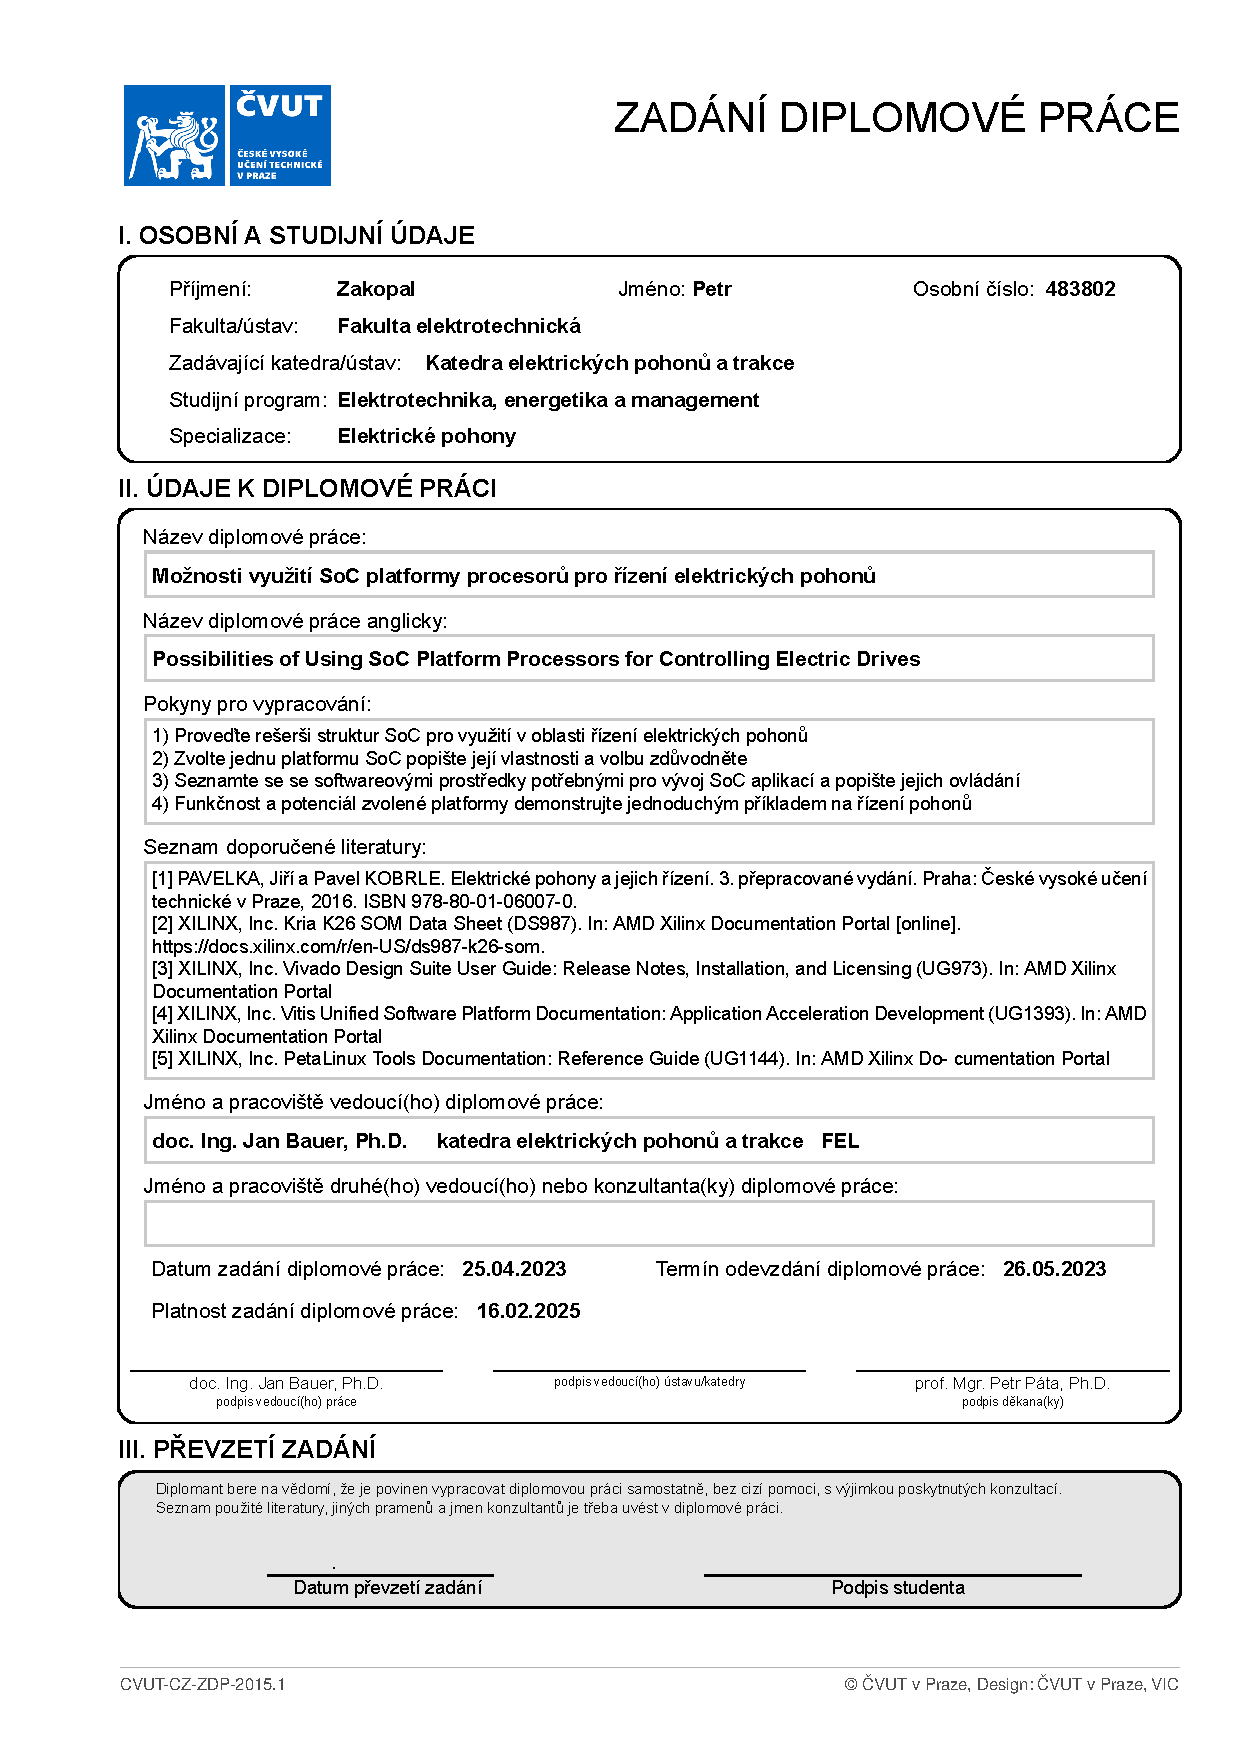
\includepdf[]{src/docs/zadani_bez_podpisu.pdf}

%\newpage
%\cleardoublepage
\null\newpage

\pagenumbering{Roman}
\setcounter{page}{5}%%3 NUTNO řešit dle zadání etc.

\noindent \textcolor{ctublue}{{\Large{\textbf{\MakeTextUppercase{Prohlášení}}}}}\\
			Prohlašuji, že jsem předloženou práci vypracoval samostatně a že jsem uvedl veškeré použité informační zdroje v~souladu s~Metodickým pokynem o~dodržování etických principů při přípravě vysokoškolských závěrečných prací.\\
		\vspace{1.5cm}
		
	

	\noindent	V~Praze dne \rule{3.5cm}{0.4pt} \hspace{6.6cm}  \rule{4cm}{0.4pt}
	
	\hspace{12.65cm}Petr Zakopal


		\vspace{14cm}
		
	\noindent	\textcolor{ctublue}{{\Large{\textbf{\MakeTextUppercase{Poděkování}}}}}\\
	Tímto bych rád poděkoval vedoucímu této práce doc. Ing. Janu Bauerovi, Ph.D. za skvělé vedení práce a cenné rady při jejím vytváření. Dále bych rád poděkoval všem, kteří mě v~mém dosavadním studiu podporovali.
		


%%ABSTRAKT%%

\newpage
%\addcontentsline{toc}{section}{3\quad Abstrakt a klíčová slova}%Added citations to TOC%
%\begin{comment}
\begin{minipage}[t]{7.37cm}
		%\raggedright
	\textcolor{ctublue}{\Large{\textbf{\MakeTextUppercase{Abstrakt}}}}\\
	Cílem této práce je prozkoumat možnosti využití heterogenních platforem \gls{abbreviation:soc} s~\gls{abbreviation:fpga} pro realizaci výpočtů v~reálném čase, zejména pro řízení elektrických pohonů a pro analýzu výkonových prvků pomocí \gls{abbreviation:hil}. V~textu jsou prezentovány postupy, které vedou k~úspěšnému vytvoření \gls{abbreviation:fpga} akcelerované aplikace, realizované na vývojové desce Xilinx Kria KR260 s~K26~\gls{abbreviation:som}. K~vytvoření akcelerované aplikace byly využity \gls{abbreviation:sw} nástroje PetaLinux, Vivado a~Vitis~\gls{abbreviation:ide}. V~rámci práce byla vytvořena aplikace simulující řízení asynchronního motoru pomocí \gls{abbreviation:foc}. Zvolené řešení akcelerované aplikace neposkytuje uspokojující výsledky ohledně rychlosti zpracování dat v~reálném čase. V~závěru práce je navrhováno řešení, které by v~případě realizace mohlo splnit daná časová omezení. Na základě vytvořené práce je možné získat přehled o~postupu tvorby akcelerované aplikace na platformě firmy Xilinx, Inc.\\
	\textbf{Klíčová slova:} \gls{abbreviation:soc}, \gls{abbreviation:mpsoc}, Xilinx, Kria KR26, Kria K26, ZynQ, \gls{abbreviation:fpga}, heterogenní systém, \gls{abbreviation:hil}, Hardware in the loop, hardwarová akcelerace, PetaLinux, Vitis, Vivado, \gls{abbreviation:hls}, High Level Synthesis, \gls{abbreviation:rtl}, řízení elektrických pohonů, kernel, Real Time Linux Patch, \gls{abbreviation:spi}, \gls{abbreviation:foc}, simulace, Field Oriented Control.
\end{minipage}%
\hfill% --- important, otherwise it wont be so nice
\begin{minipage}[t]{7.37cm}
		\textcolor{ctublue}{\Large{\textbf{\MakeTextUppercase{Abstract}}}}\\
		The goal of this thesis is to research the possibilities of using heterogeneous platforms consisting of \gls{abbreviation:soc} with \gls{abbreviation:fpga} for making real-time calculations, which could be utilized for controlling electric drives or/and analysing the behaviour of power electronic parts. The text describes the flow of creating the accelerated applications on the Xilinx Kria KR260 development board which utilizes the K26 \gls{abbreviation:som}. The PetaLinux, Vivado and Vitis \gls{abbreviation:ide} tools were used for creating the \gls{abbreviation:fpga} accelerated application. The possibilities were demonstrated by an application which simulates the \gls{abbreviation:foc} of an induction motor. The used solution of accelerated appliaction does success in maintaining the time constraints needed for real-time calculations. However, at the end of the thesis the author presents creating another solution, which could be utilised to meet the given time constraints for real-time applications. By following the text, the reader can gain insight on how to develop a basic accelerated application utilizing Xilinx, Inc. development board.\\
		\textbf{Keywords:} \gls{abbreviation:soc}, \gls{abbreviation:mpsoc}, Xilinx, Kria KR26, Kria K26, ZynQ, \gls{abbreviation:fpga}, heterogeneous system, \gls{abbreviation:hil}, Hardware in the loop, hardware acceleration, PetaLinux, Vitis, Vivado, \gls{abbreviation:hls}, High Level Synthesis, \gls{abbreviation:rtl}, electric drives control, kernel, Real Time Linux Patch, \gls{abbreviation:spi}, \gls{abbreviation:foc}, simulation, Field Oriented Control.
\end{minipage}
%\end{comment}
	%\textcolor{ctublue}{\Large{\textbf{\MakeTextUppercase{Abstrakt}}}}\\

	%\textcolor{ctublue}{\Large{\textbf{\MakeTextUppercase{Abstract}}}}\\

\newpage
\tableofcontents
\newpage%
\flushbottom %vyčištění stránky
\newpage
\vspace{0pt}
\listoffigures %seznam obrázků
\flushbottom %vyčištění stránky
\newpage
\listoftables
\flushbottom
\newpage


\pagenumbering{arabic} %to arabic page numbering - enabling page numbering after gobble which disabled page numbering
\pagenumbering{gobble}
\null\newpage
% \null\newpage %PŘI VERZI ONLINE
\setcounter{page}{1}
\pagenumbering{arabic}
\fontspec{Times New Roman}

\section{Úvod}
V~době, kdy byla od elektrických pohonů požadována spolehlivost, vysoká účinnost a výpočetně nenáročné, ovšem kvalitní řízení, byly k~řízení využívány konvenční digitální signálové procesory (\gls{abbreviation:dsp}). Postupem času však docházelo ke zjištění, že výkon \gls{abbreviation:dsp} nemusí být dostatečný, zejména pro aplikace, u~kterých je vyžadováno provést velké množství náročných výpočtů za co nejkratší čas. Aktuálně nastupuje éra \gls{abbreviation:soc}, které v~mnoha případech obsahují heterogenní strukturu řídící procesorové jednotky (\gls{abbreviation:cpu}) a logického programovatelného pole (\gls{abbreviation:fpga}). Implementace hradlových polí přináší nejen v~řízení elektrických pohonů zvýšení výpočetního výkonu, ale také snížení energetické náročnosti.\par
Perspektiva \gls{abbreviation:soc} a \gls{abbreviation:fpga} je podpořena jejich využíváním i mimo obor elektrických pohonů. Z~důvodu vysoké propustnosti \gls{abbreviation:fpga}, vysokých výpočetních výkonů a nízké energetické náročnosti jsou využívány v~\gls{abbreviation:ai}, machine learningu, zpracování obrazu a jiných nepohonářských aplikacích.\par
Náročnější postup designování logiky a algoritmů aplikací v~\gls{abbreviation:fpga} může představovat problém v~jejich implementaci. Aplikace je tvořena postupem, který kladne vysoké nároky na vzdělání a zkušenosti vývojářů. Většina \gls{abbreviation:fpga} je designována pomocí jazyků Verilog či \gls{abbreviation:vhdl}, jejichž použití a filozofie mohou pro softwarově orientované programátory představovat značnou překážku. Proto je v~poslední době trend tvořit aplikace pomocí vyšší úrovně syntézy (\gls{abbreviation:hls}). Při použití \gls{abbreviation:hls} je možné tvořit programy ve vyšších programovacích jazycích jako je například C, C++ či Python. Vytvořený kód je přeložen do úrovně registrů (\gls{abbreviation:rtl}), která je následně syntetizována, implementována a generována do bitstreamu, který slouží ke konfiguraci cílového \gls{abbreviation:fpga} zařízení.\par
V~prvních kapitolách této práce jsou v~teoretické úrovni představeny \gls{abbreviation:soc}, \gls{abbreviation:fpga} a jejich možné využití v~pohonářských i nepohonářských aplikacích. Z~mnoha dostupných produktů na trhu byly vybrány platformy Xilinx Kria KR260 \gls{abbreviation:som} a Digilent Zybo Zynq-7000. Platformy byly vzájemně porovnány z~různých hledisek a pro demonstraci možného využití platformy pro simulaci asynchronního motoru řízeného pomocí \gls{abbreviation:foc} byla vybrána platforma Xilinx Kria KR260.\par
V~navazujících kapitolách je čtenářovi představen postup, kterým je možné vytvořit kompletní akcelerovanou aplikaci s~použitím nástrojů \textit{PetaLinux}, Vivado a Vitis \gls{abbreviation:ide}.\par
V~závěru práce je představena realizace akcelerované aplikace, která je schopna využívat \gls{abbreviation:spi} komunikaci s~externími zařízeními. Pro \gls{abbreviation:spi} komunikaci byl vytvořen hardware (\gls{abbreviation:hw}) přímo v~\gls{abbreviation:fpga}, který je ovládán z~prostředí (user space) aplikace. Na základě analýzy aplikace bylo vyhodnoceno, zda způsob vybrané realizace je vhodný pro provádění výpočtů v~reálném čase.

\flushbottom %vyčištění stránky
\newpage
%konec úvodu

\section{System on a chip}\label{sec:system-on-a-chip}
	% co to je, proč to je
	% typy postavené kolem  mikrokontroléru, mikroprocesoru a ASIC
	% Aplikace Embedded system (existují i pro mobilní aplikace, osobní počítače)
	System on a chip (\gls{abbreviation:soc}) je struktura, využívající integrování různých prvků systému na jeden čip. Integrace prvků na jeden čip značně snižuje nároky na rozměry nosičů, na kterých jsou tyto \gls{abbreviation:soc} umístěny. Místo diskrétních čipů, obstarávající jednotlivé funkce, je využito jednoho čipu s~integrovanými prvky, které vykonávají požadované funkce.\par
	Při integrování prvků do jedné polovodičové struktury dochází ke značnému snížení potřebných počtů kovových vodivých spojů, snížení časové náročnosti výroby a zvýšení rychlosti přenosu dat. Proto je \gls{abbreviation:soc} upřednostňováno před metalicky spojenými diskrétními prvky, vykonávající dané operace.\par
	Označení \gls{abbreviation:soc} může představovat mnoho struktur. Obecné rozdělení, které je možné naleznout v~literatuře a veřejných zdrojích, je následující \cite{tomshardware-system-on-chip}:
	\begin{itemize}
		\item \gls{abbreviation:soc} využívající mikrokontroléru (obsahující \gls{abbreviation:cpu}, \gls{abbreviation:ram}, \gls{abbreviation:rom}),
		\item \gls{abbreviation:soc} využívající pouze mikroprocesoru (obsahující \gls{abbreviation:cpu}, možné i \gls{abbreviation:gpu}, jádra pro specializované výpočty),
		\item \gls{abbreviation:soc} určené pro specifické aplikace (Application Specific Integrated Circuit – \gls{abbreviation:asic}).
	\end{itemize}\par
	Z~uvedených rozdělení jsou pro řízení elektrických pohonů nejvíce využívány \gls{abbreviation:soc} s~mikrokontrolérem a \gls{abbreviation:asic}.

	\subsection{Application Specific Integrated Circuit}
		Významnou část \gls{abbreviation:soc} tvoří \textit{Application Specific Integrated Circuits, popř. Hardware} (\gls{abbreviation:asics}, \gls{abbreviation:ashw}). Při použití těchto \gls{abbreviation:soc} je předpokládáno, že pokud je architektura \gls{abbreviation:hw} specializovaná přímo na vykonávání jedné aplikace, je vysoká pravděpodobnost, že ji bude vykonávat bezchybně, kvalitně a rychle.\par
		Tyto aplikace jsou využívány v~širokém spektru oborů, jako je např. zpracování zvuku, videa, výpočtů. Tyto \gls{abbreviation:asic} mohou vykonávat rychlé výpočty pro matematické modely elektrických strojů, které jsou využívány např. pro \gls{abbreviation:hil}.\par
		Než je \gls{abbreviation:asic} určen pro velkoprodukci, je nutné jej navrhnout, vyzkoušet a odladit. K~tomu slouží např. logická programovatelná pole (\gls{abbreviation:fpga}). Pokud velkoprodukce není z~ekonomických důvodů možná, jsou \gls{abbreviation:fpga} využívána přímo v~produkci. Pomocí nich je vytvořena \gls{abbreviation:hw} struktura, která by byla přítomna na \gls{abbreviation:asic}.


	\subsection{Aplikace SoC}
	Systémy na čipu se pro jejich výpočetní výkon, prostorovou a energetickou efektivnost využívají v~mnoha aplikacích. Jedno z~nejvýznamnějších využití v~oboru elektrických pohonů je v~embedded systémech a hardwarově akcelerovaných aplikacích.

\section{System on Modules}\label{sec:system-on-modules}

	System on modules (\gls{abbreviation:soms}) je struktura, jejíž hlavní součástí je \gls{abbreviation:soc}. \gls{abbreviation:soms} se oproti \gls{abbreviation:soc} již dodávají na \gls{abbreviation:pcb} a kromě \gls{abbreviation:soc} mají na \gls{abbreviation:pcb} umístěny další komponenty, které mohou být pro danou aplikaci vyžadovány. \cite{xilinx-what-is-a-som}\par
	\gls{abbreviation:soms} se mohou dodávat jako vývojové desky \cite{xilinx-kria-kr260-robotics-starter-kit}, které obsahují kromě \gls{abbreviation:soms} také nosnou desku (tzv. Carrier Card, \gls{abbreviation:cc}) s~dalšími komponenty, jež jsou vhodné pro vývoj standardních aplikací. Pokud zákazník pomocí vývojové desky odladil vyvíjenou aplikaci, může zakoupit samostatný \gls{abbreviation:som} na základní desce (base board, \gls{abbreviation:bb}) a \gls{abbreviation:cc} pro danou aplikaci navrhnout tak, aby obsahovala pouze komponenty, které daná aplikace využívá. Tímto způsobem je možné snížit cenu konečného výrobku o~komponenty, které byly z~\gls{abbreviation:cc} při návrhu odstraněny pro jejich nevyužití. Ovšem při tomto způsobu realizace dochází ke zvýšení finanční a časové náročnosti vývoje.\par
	Výrobce platformy \textit{Kria KR260 Robotics Starter Kit}, použité v~této práci, dodává k~produktu rozsáhlou dokumentaci \cite{kria-som-carrier-card-design-guide-2022}, \cite{kria-k26-som-ds}, podle které je možné individuální \gls{abbreviation:cc} sestavit. \par
	Příkladem individuálně vytvořené \gls{abbreviation:cc} je open source projekt od firmy \textit{Antmicro Ltd}. Tato firma vydala open source design \gls{abbreviation:cc} pro \textit{K26 SOM}, původně využívané na \textit{Kria KV260}, jež je určen pro akcelerování audiovizuálních aplikací. Individuální design využívá totožný \gls{abbreviation:soms}, jako je použit v~této práci, ale rozdílný \gls{abbreviation:cc}. Dokumentace a vytvořený návrh je dostupný v~\cite{antmicro-open-source-kria-k26-carrier-card}.

	\subsubsection{Embedded Systems}
	Embedded systems je název pro skupinu prvků, obecně systémů, které je možné charakterizovat jako specifické výpočetní zařízení, resp. počítače, které jsou určeny pro podporu funkce nebo řízení nějakého většího celku, produktu, nebo fyzikálního systému. Naopak osobní počítač je výpočetní zařízení, které je určeno pro vykonávání mnoha univerzálních aplikací a funkcí, které nejsou v~okamžiku vývoje počítače určeny, proto nelze mluvit o~embedded systému. \cite{Sass2010}\par
	Dalším důležitým rozdílem mezi \textit{Embedded System} a obecným výpočetním zařízením je ten, že v~případě embedded systému je interakce mezi systémem a uživatelem uměle omezena na základní ovládání či kontrolu funkce. Není předpokládáno, že by uživatel, jež aplikaci embedded systému využvá, výrazným způsobem zasahoval do jeho funkce. Naopak obecný výpočetní systém je uzpůsoben na podstatné zásahy uživatele. \cite{Sass2010} \cite{juan-fpgas}\par
	Do embedded systému vstupují signály, které jsou v~něm zpracovány a vybrané výsledky výpočtů jsou výstupním produktem systému (v~podobě výstupních signálů). Tyto produkty mohou pomocí akčních členů zasahovat do řízeného systému. Vstupní signály jsou většinou získávány ze speciálních snímačů, kompatibilních s~embedded systémem (senzor teploty, senzor tlaku, senzor zrychlení, gyroskop, senzory proudu, inkrementální čidla apod.). Jeho výstupní signály jsou například specifická ovládací hodnota napětí, proudu nebo jiné veličiny. Na výstupních pinech mohou být také připojené \gls{abbreviation:led} signalizace, komunikační sběrnice některých komunikačních systémů nebo \gls{abbreviation:lcd} displeje. Způsob, kterým jsou kódovány vstupní a výstupní signály, je většinou specificky určen řízeným systémem. \cite{Sass2010}\par
	K~obecnému výpočetnímu systému je možné připojit vstupní periferie klasických osbních počítačů (myš, klávesnice, mikrofon). Komunikace embedded systému s~periferiemi je většinou standardizována tak, aby bylo možné periferie libovolně zaměňovat beze změny funkčnosti. \cite{Sass2010}.\par
	Na obrázku \ref{fig:embedded-system-scheme} je zobrazeno blokové schéma řízení fyzikálního systému pomocí embedded systému. Tyto bloky mezi sebou komunikují pomocí digitálních signálů. Pokud tyto signály nejsou digitální, musí se před zpracováním v~embedded systému zdiskretizovat.

	\begin{figure}[htbp!]
		\centering
			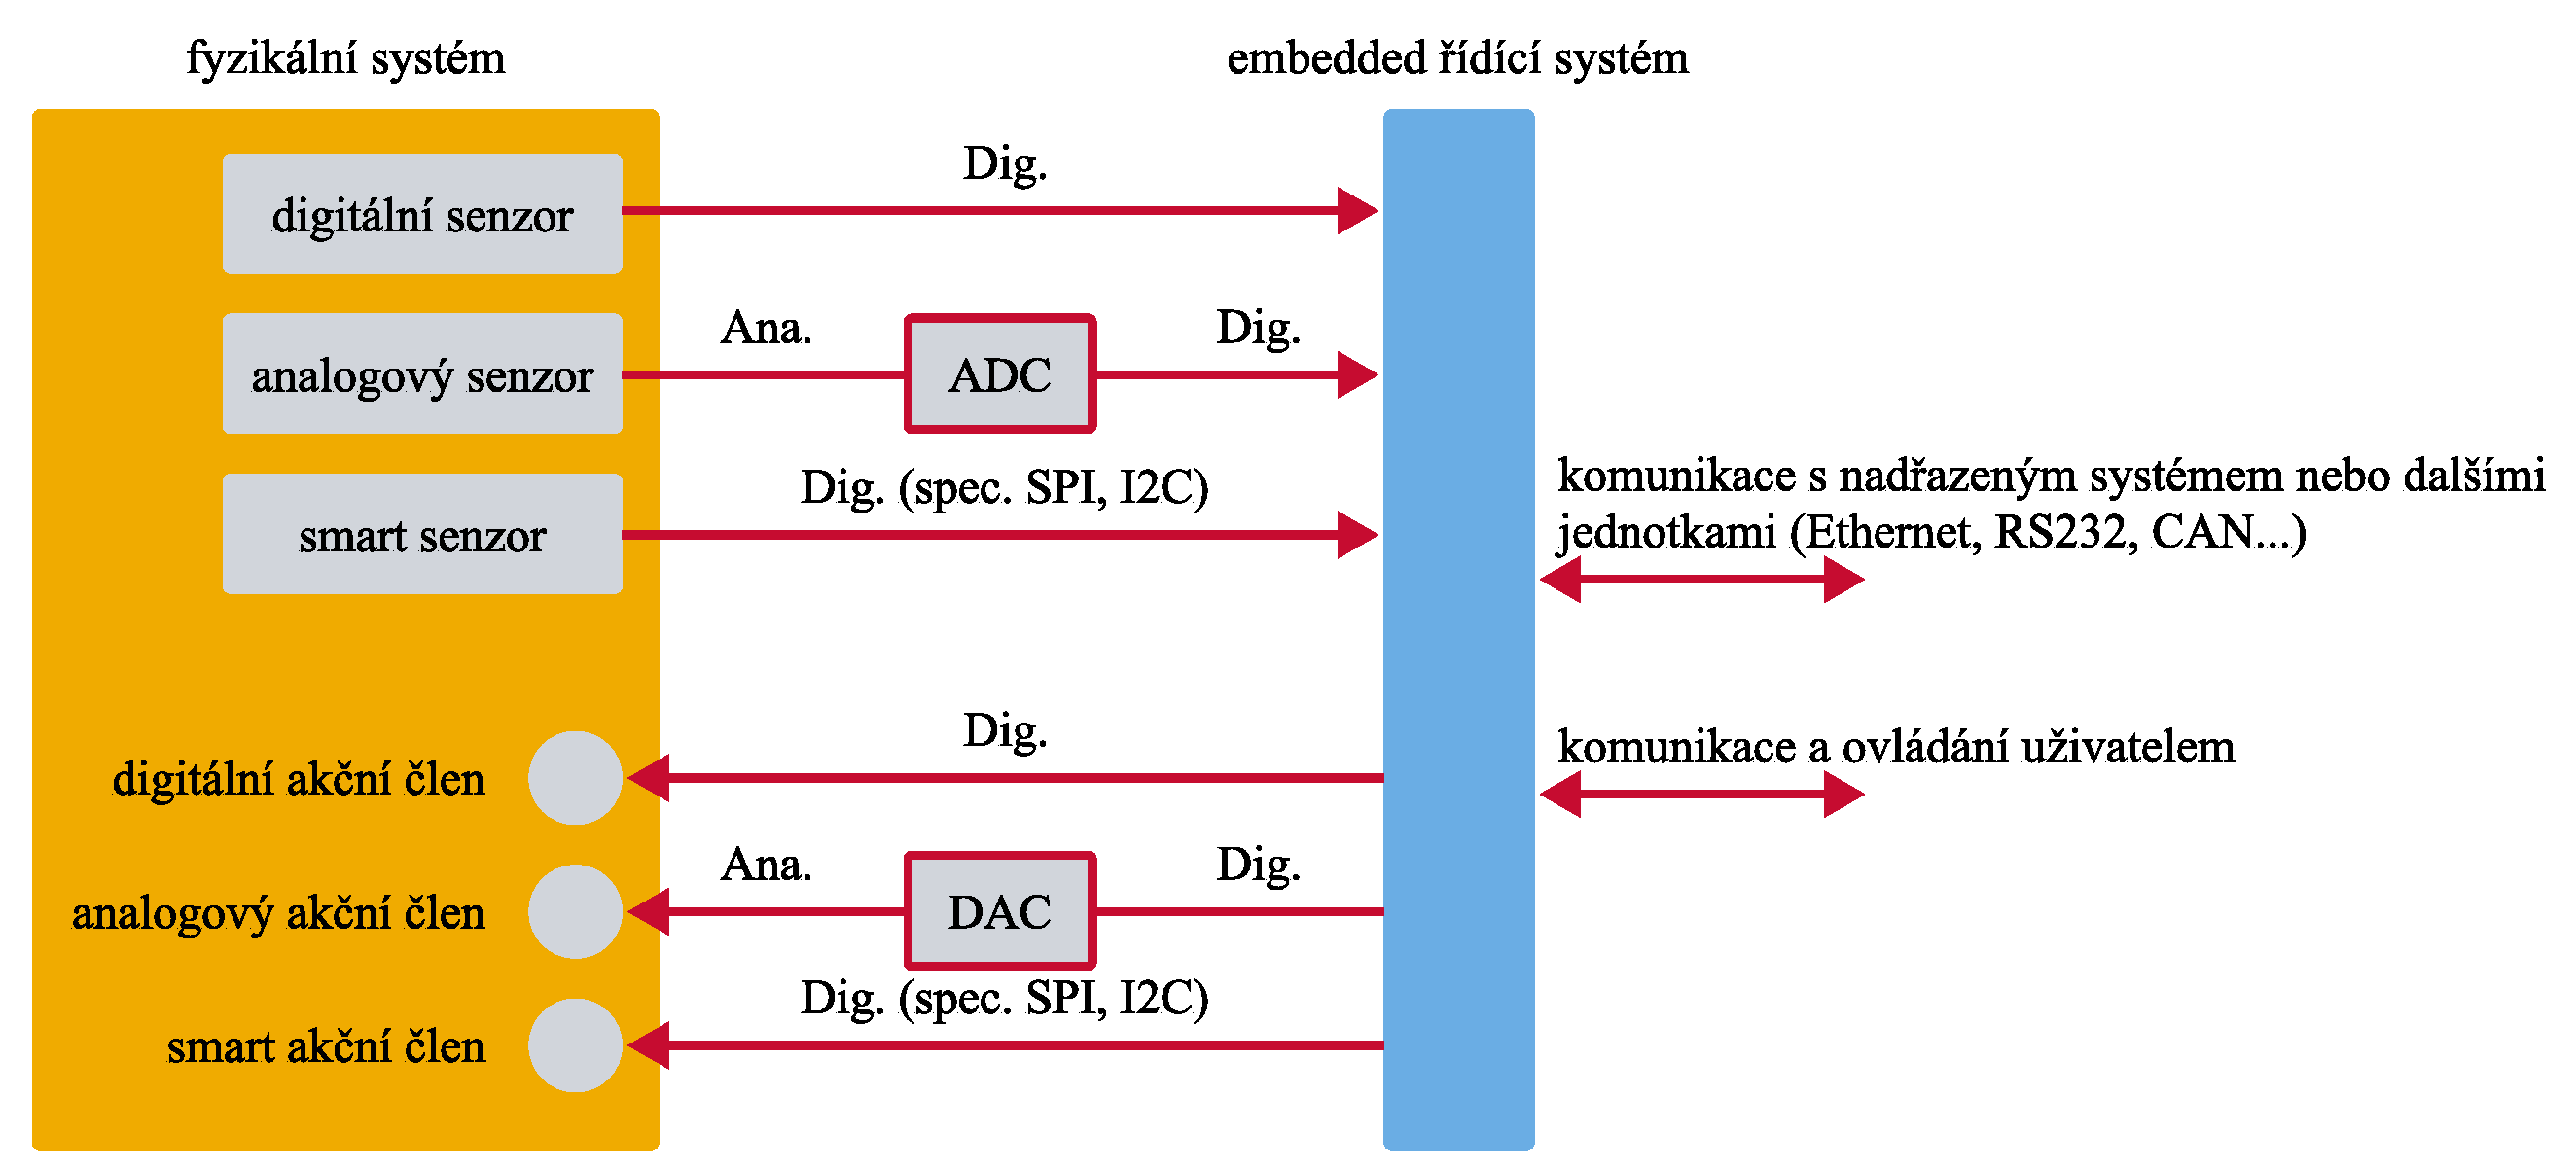
\includegraphics[width=1\textwidth]{src/pdf/embedded-system-scheme.pdf} 
			\caption{Blokové schéma embedded systému a řízeného fyzikálního systému. (převzato z~\cite{juan-fpgas}, upraveno)}
			\label{fig:embedded-system-scheme}
	\end{figure}

		\fbar

		\subsubsection{Hardware Accelerated Applications}\label{subsec:hardware-accelerated-applications}
		V~mnoha aplikacích je vyžadováno, aby výpočty nebo zpracování dat probíhalo vysokou rychlostí. Tento problém je v~některých případech problematické řešit použitím běžného procesoru (\gls{abbreviation:cpu}), který je optimalizován na provádění obecných komplexních funkcí, řízení běhu uživatelského programu, komunikaci či přesun dat. V~moderním světě je třeba zpracovávat množství dat, které v~některých případech exponenciálně narůstá. Aby tyto data bylo možné v~požadovaném čase s~co nejnižším zpožděním zpracovat, je vhodné využít specifický \gls{abbreviation:hw} a přístup, který bude schopen požadavky rychlosti a výkonu uspokojit. Tento přístup se nazývá \textit{Hardware Acceleration} (hardwarová akcelerace). \cite{xilinx-accelerated-computing}\par
		Princip hardwarové akcelerace spočívá v~přesunu výpočetně náročných aktivit na specifický a oddělený hardware. Celkové řízení běhu aplikace a komunikace je ovšem stále vykonáváno řídícím \gls{abbreviation:cpu}. Oddělený hardware, na kterém dochází k~akceleraci výpočtů, je optimalizován na vykonávanou úlohu a jeho využití přináší zefektivnění běhu celé aplikace. \cite{xilinx-accelerated-computing}\par
		Struktura, ve které je využíváno více fyzicky oddělených procesorových a hardwarových akceleračních jednotek, se často nazývá heterogenní. \cite{xilinx-accelerated-computing}\par
		Hardwarová akcelerace je schopna poskytovat rychlejší výpočty než \gls{abbreviation:cpu}, protože využívá maximální paralelizace výpočtů. Klasické \gls{abbreviation:cpu} však vykonává jednotlivé instrukce sériově. V~případě, že \gls{abbreviation:cpu} využívá pro výpočty více jader a vláken, je velmi náročné se úrovní paralelizace, při dodržení stejné energetické náročnosti, vyrovnat výpočtům pomocí \gls{abbreviation:hw}.
		Pro \gls{abbreviation:hw} akceleraci je v~mnoha oblastech využíváno několik druhů jednotek, které jsou optimalizovány pro dané charaktery aplikací.\par
		\textbf{Graphics Processing Units} (\gls{abbreviation:gpus}) jsou jednotky, které slouží převážně k~akceleraci zpracovávání vizuálních úloh. V~době rapidního rozvoje elektroniky a \gls{abbreviation:sw} je možné využít \gls{abbreviation:gpus} v~mnoha odvětví umělé inteligence (\gls{abbreviation:ai}) či kreativních odvětích. \gls{abbreviation:gpus} jsou využívány v~aplikacích, kde není kladen veliký důraz na nízkou odezvu (latenci). \cite{xilinx-accelerated-computing}\par
		\textbf{Tensor Processing Units} (\gls{abbreviation:tpus}) jsou jednotky, které slouží k~provádění algoritmů strojového učení (machine-learning, \gls{abbreviation:ml}). Jejich přímé datové propojení umožňuje velmi rychlý a přímý přenost dat. Díky přímému připojení nevyžadují využití pamětí, které by přenos dat zpomalovaly. \cite{xilinx-accelerated-computing}\par
		\textbf{Field Programmable Gate Arrays} (\gls{abbreviation:fpgas}) jsou jednotky, ve kterých není při výrobě pevně daná \gls{abbreviation:hw} struktura. To umožňuje vytvoření, resp. nakonfigurování \gls{abbreviation:hw} dle požadavků akcelerované aplikace. \gls{abbreviation:fpgas} mohou být využívány i při výpočtech matematických modelů elektrických strojů v~reálném čase. Při realizaci této práce je pro akceleraci využíváno právě těchto programovatelných polí.\\ \\
		\noindent Vhodným příkladem porovnání časové náročnosti matematických výpočtů pro selektivní eliminaci harmonických složek v~trakci pomocí \gls{abbreviation:cpu} a \gls{abbreviation:gpu} je provedeno v~\cite{ieee-selective-harmonic-elimination-nvidia}.\par
		Z~článku vyplývá že využitím \gls{abbreviation:gpu} skutečně dochází ke~snížení potřebného času na provedení výpočtu. V~některých případech se jedná o~snížení výpočetního času ze~183~ms (při použití \gls{abbreviation:cpu}) na 0,81~ms (při použití NVIDIA Titan V~GPU). Díky využití \gls{abbreviation:gpu} je tedy možné algoritmus v~lokomotivě provádět v~reálném čase.

	\subsubsection{Výpočetní technika, mobilní zařízení a elektronika}
	Kromě průmyslových odvětví jsou \gls{abbreviation:cpu} využívány i pro běžné aplikace spotřební elektroniky.\par
	Protože jsou kladeny stále vyšší nároky na výpočetní rychlost a nižší cenu ve spotřební elektronice, jako jsou mobilní zařízení (mobilní telefony, osobní počítače), servery, začíná převažovat využívání \gls{abbreviation:soc} i v~těchto oblastech.\par
	Společnost Apple Inc. již téměř ve všech novějších zařízeních používá individuálně navrhnutý \gls{abbreviation:soc}.
	Příkladem je A16 Bionic pro iPhone 14 Pro, Apple M1 a M2 pro tablety a počítače.\par
	Díky specifickým řešením a vylepšeným architekturám (jádra \gls{abbreviation:soc} pro vysoký výkon a jádra pro ekonomickou spotřebu energie) bylo možné zvýšit výkon a snížit energetickou náročnost zařízení spotřební elektroniky. \cite{apple-explore-the-new-architecture-of-apple-silicon-macs}


	\section{Programovatelné hradlové pole – FPGA}
		\subsection{Vývoj FPGA z~PLD}
		Programovatelná hradlová pole (\gls{abbreviation:fpga}) jsou zařízení, jejichž historický vývoj stojí na programovatelných logických zařízení (programmable logic devices, \gls{abbreviation:pld}). První \gls{abbreviation:pld} fungovala na principu Booleových funkcí součtu násobení (sum of products). Tato zařízení obsahovala matici (proto se také nazývají programmable logic arrays, \gls{abbreviation:pla}) více vstupových bloků AND a OR. Programování požadované funkce probíhalo pomocí přerušování vstupů do jednotlivých logických bloků. Později byly do struktury \gls{abbreviation:pla} přidány D~klopné obvody s~multiplexory. Díky těmto součástím bylo možné vytvářet logické kombinační a sekvenční obvody, resp. automaty. Posledním vylepšením \gls{abbreviation:pla}, které stálo před zrodem \gls{abbreviation:fpga}, spočívalo v~umístění více \gls{abbreviation:pla} bloků (skládajících se z~AND, OR, multiplexeru a D klopného obvodu) na jeden integrovaný čip. Programovatelné spojení různých \gls{abbreviation:pla} bloků a výstupů umožnilo vytvořit požadovanou funkci. \cite{Sass2010}\par

		\subsection{Aktuální složení FPGA}
		Moderní \gls{abbreviation:fpga} se skládají z~2D matice propojených programovatelných logických bloků, bloků speciálních funkcí a propojů. Logické bloky se skládají z~mnoha buněk, které se skládají z~generátorů funkcí a paměťových elementů. Po obvodě \gls{abbreviation:fpga} jsou rozmístěny vstupní a výstupní piny (\gls{abbreviation:io}), připojené na zvláštní logické bloky. \cite{Sass2010}\par
		Na obr. \ref{fig:fpga-general-design} je možné pozorovat schéma základního konceptu uspořádání \gls{abbreviation:fpga}. Na schématu jsou vyznačeny logické bloky, jejich propojení, propojovací matice pro aktivování jednotlivých propojů a vstupů a výstupů (\gls{abbreviation:io}) \gls{abbreviation:fpga}.\par
		I~přesto, že se tato práce převážně věnuje využití \gls{abbreviation:soc} a \gls{abbreviation:soms} pro řízení elektrických pohonů je vhodné představit základní části \gls{abbreviation:fpga} a nastínit jejich funkci.

		\begin{figure}[htbp!]
			\centering
				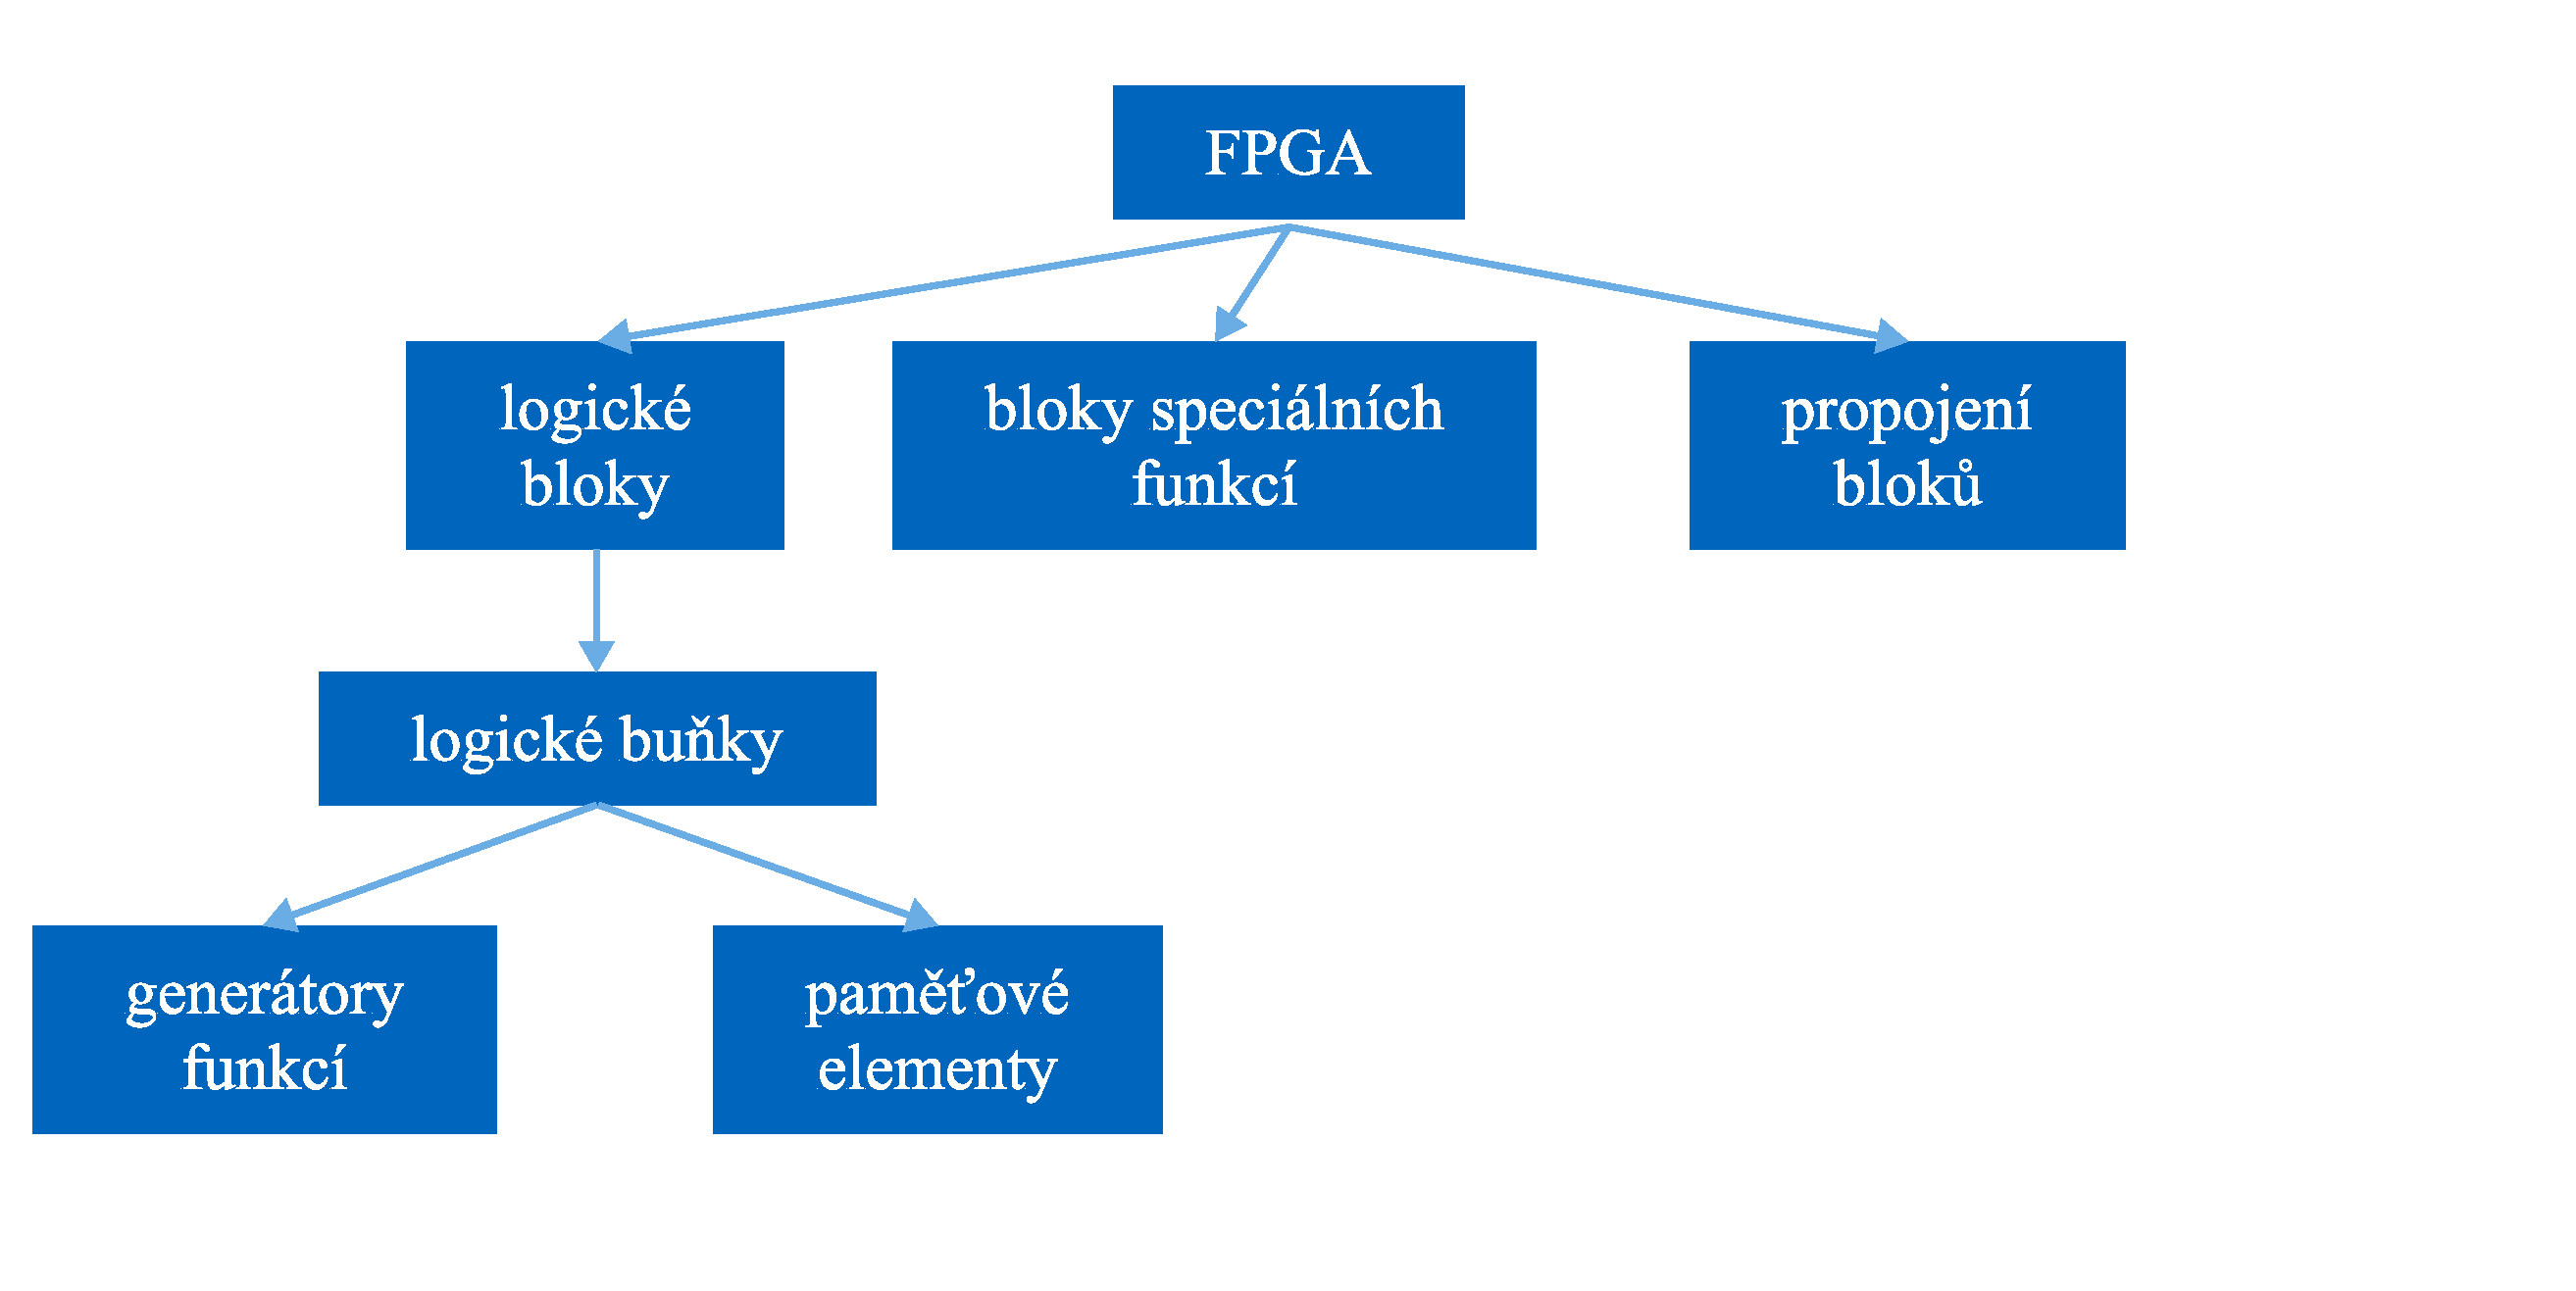
\includegraphics[width=1\textwidth]{src/pdf/fpga-skladba.pdf} 
				\caption{Blokové schéma složení moderních \gls{abbreviation:fpga}.}
				\label{fig:fpga-skladba}
		\end{figure}


		\begin{figure}[htbp!]
			\centering
				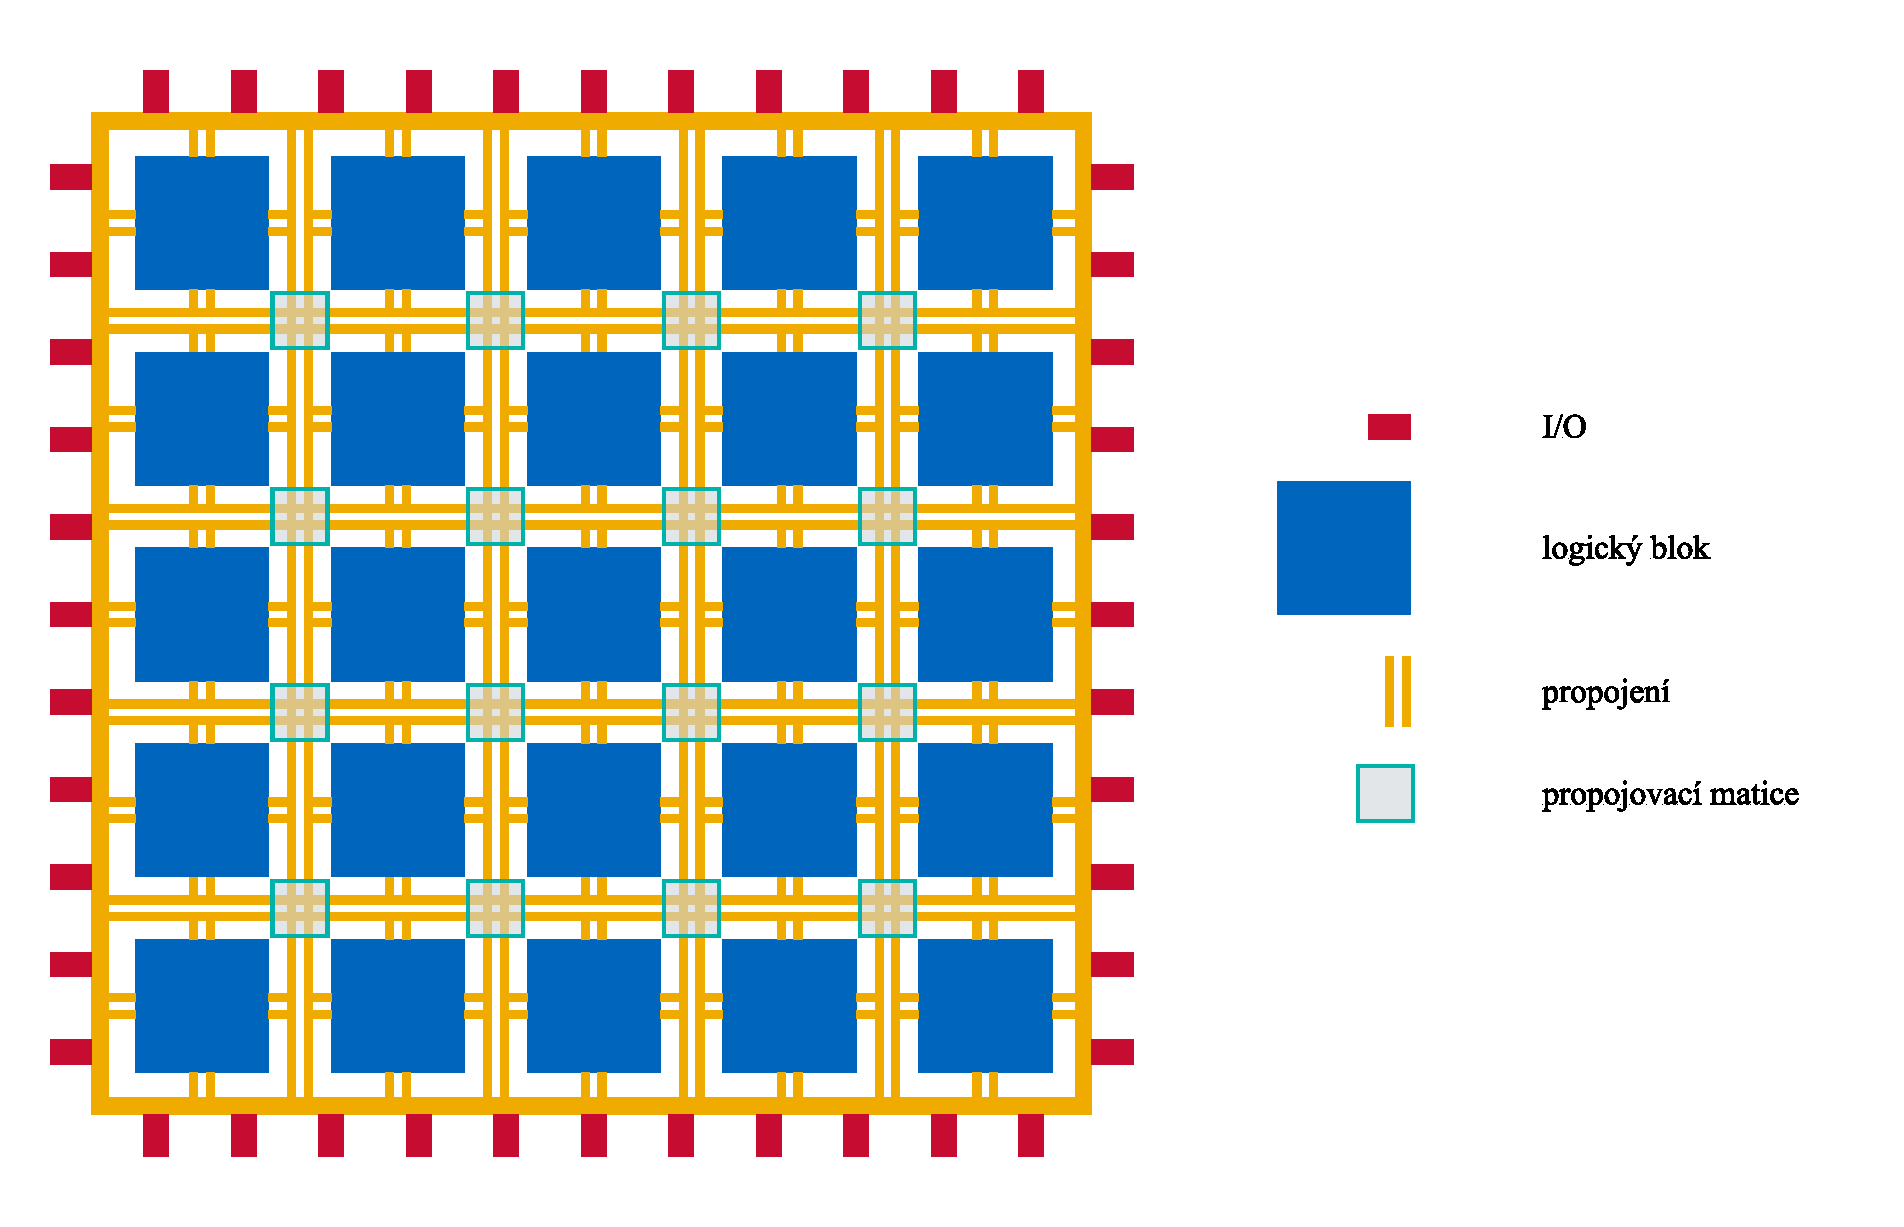
\includegraphics[width=1\textwidth]{src/pdf/fpga-general-design.pdf} 
				\caption{Základní koncept uspořádání \gls{abbreviation:fpga}.}
				\label{fig:fpga-general-design}
		\end{figure}

		\fbar
		\subsubsection{Generátory funkcí}\label{subsubsec:generatory-funkci}
		Oproti předchůdcům (\gls{abbreviation:pld}), které pro generování funkcí používaly logická hradla tvořená \gls{abbreviation:cmos} tranzistory, využívají \gls{abbreviation:fpga} tzv. generátory funkcí.\par
		Logickou funkci je možné popsat pravdivostní tabulkou, která má určitý počet vstupů a odpovídající počet výstupů. Dle \cite{Sass2010} je možné si představit, že se generátor dané funkce skládá ze samostatné statické paměti (\gls{abbreviation:sram}), jejíž výstupy jsou přímo přivedeny na vstup multiplexeru (\gls{abbreviation:mux}). Signály výběru výstupů by odpovídaly vstupním proměnným a jednotlivé vstupy do \gls{abbreviation:mux} výstupům funkce.\par
		Pro bližší pochopení generátoru funkcí z~předchozího odstavce je možné představit realizaci smyšlené logické funkce $\text{f} (x, y, z) = \bar{x}z + y$. Pravdivostní tabulka této smyšlené logické funkce je zobrazena v~tab.~\ref{tab:fpga-pravdivostni-tabulka-smyslene-funkce-generatoru-funkci}. Odpovídající realizace pomocí \gls{abbreviation:mux} a \gls{abbreviation:sram} je zobrazena na obr. \ref{fig:fpga-function-generator}. Tato reprezentace se nazývá look-up table (\gls{abbreviation:lut}). Grafické znázornění je inspirováno \cite{Sass2010}.
		

	\begin{minipage}[t]{0.45\textwidth}
		\begin{table}[H]
			\centering
			\caption{Pravdivostní tabulka ukázkové funkce, realizované v~generátoru funkcí, umístěném v~logickém bloku \gls{abbreviation:fpga}.}
		  \vspace*{0.15cm}
		
			\begin{tabular}{!{\vrule width 2pt} c | c | c | c !{\vrule width 2pt} c !{\vrule width 2pt}}
			\noalign{\hrule height 2pt}
			\rowcolor{codeblue}
			$i$ & $x$ &	$y$ & $z$ & f($x,y,z$)\\
			\noalign{\hrule height 2pt}
			0 & 0 & 0 & 0 & 0\\ \hline
			1 & 0 & 0 & 1 & 1\\ \hline
			2 & 0 & 1 & 0 & 1\\ \hline
			3 & 0 & 1 & 1 & 1\\ \hline
			4 & 1 & 0 & 0 & 0\\ \hline
			5 & 1 & 0 & 1 & 0\\ \hline
			6 & 1 & 1 & 0 & 1\\ \hline
			7 & 1 & 1 & 1 & 1\\\noalign{\hrule height 2pt}
			\end{tabular}
			\label{tab:fpga-pravdivostni-tabulka-smyslene-funkce-generatoru-funkci}
		\end{table}
	\end{minipage}%
	\hfill% --- important, otherwise it wont be so nice
	\begin{minipage}[t]{0.45\textwidth}
		\begin{figure}[H]
			\centering
				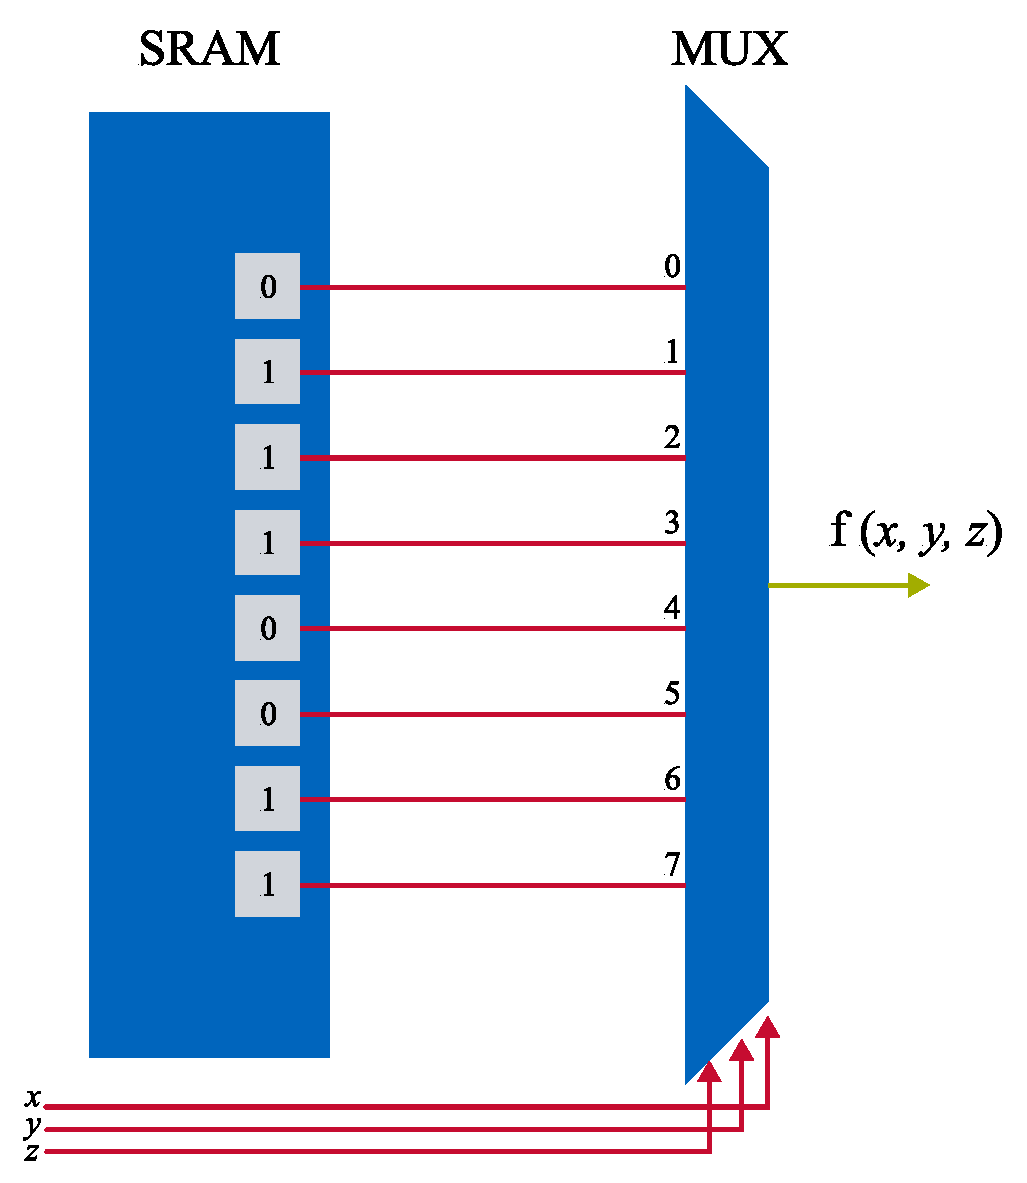
\includegraphics[width=1\textwidth]{src/pdf/fpga-function-generator.pdf} 
				\caption{Ukázka, jakým způsobem realizuje funkční generátor požadovanou funkci pomocí \gls{abbreviation:sram} a \gls{abbreviation:mux}. (inspirováno \cite{Sass2010})}
				\label{fig:fpga-function-generator}
		\end{figure}
	\end{minipage}

	\vspace*{0.5cm}
	Výhoda reprezentace funkcí pomocí generátorů funkcí oproti logickým hradlům je, že doba zpoždění signálu (propagation delay) pro funkci je konstantní. Respektivě je konstantní, pokud funkci je možné realizovat jednou \gls{abbreviation:lut}. Pro relizace obecné funkce je zapotřebí multiplexer $2^{n}$ \rightarrow 1 a \gls{abbreviation:sram} s~počtem buněk $2^{n}$, kde $n$ je počet vstupních proměnných dané funkce. \cite{Sass2010}

	\subsubsection{Paměťové elementy}\label{subsubsec:pametove-elementy}
		Paměťové elementy jsou v~\gls{abbreviation:lut} realizovány pomocí D-klopných obvodů. Tyto obvody mohou při konfiguraci \gls{abbreviation:fpga} být nastaveny tak, že budou reagovat na nástupnou nebo sestupnou hranu časovacího signálu (clock, \gls{abbreviation:clk}) řídícího procesoru nebo na úroveň řídícího signálu (latch). \cite{Sass2010}\par
		Protože typ latch je citlivý na úroveň signálu, může být problematické dovést požadovaný signál na vstup klopného obvodu v~požadovaném čase. Velmi často jsou proto paměťové členy konfigurovány jako D-klopné obvody reagující na hranu. Pokud je používán signál \gls{abbreviation:clk} vyšších frekvencí, je D-klopný obvod reagující na hranu snadněji schopný reagovat v~požadovaném čase. \cite{Sass2010}\par
		Často jsou na vstup paměťových elementů připojeny výstupy \gls{abbreviation:mux} \hyperref[subsubsec:generatory-funkci]{\textit{generátorů funkcí}}. \cite{Sass2010}

		\subsubsection{Logické buňky}\label{subsubsec:logicke-bunky}
			Logické buňky jsou elementy, skládájící se z~\hyperref[subsubsec:generatory-funkci]{\textit{generátorů funkcí}} a \hyperref[subsubsec:pametove-elementy]{\textit{paměťových elementů}}. Velmi často se počet logických buněk údává jako jeden ze základních parametrů \gls{abbreviation:fpga}, podle kterého je uživatel možný rozhodnout, zda je obvod vhodný pro jeho aplikaci. Pomocí logické buňky nebo skupiny logických buněk je již možné vytvářet plnohodnotnou kombinační a sekvenčí logiku. \cite{Sass2010}

			\newpage
		\subsubsection{Logické bloky}\label{subsubsec:logicke-bloky}
			Logické bloky se skládají ze spojení několika \hyperref[subsubsec:logicke-bunky]{\textit{logických buněk}} do jedné skupiny. Díky umístění této skupiny buněk na čip geograficky blízko dochází k~minimalizaci zpoždění signálu mezi jednotlivýmy buňkami. Častá skutečnost je, že jednotlivé bloky mohou mít již předkonfigurovanou funkci, jako je např. sčítačka, dělička nebo násobička. \cite{Sass2010}

		\subsubsection{Propojení bloků}
			Propojení bloků je prováděno z~důvodu spojení jednotlivých logických bloků a \gls{abbreviation:io}. Pro spínání určených propojů jsou na čipu mezi jednotlivými propoji umístěny propojovací matice, resp. „přepínače“. Ty slouží ke spojení jinak oddělených propojů, logických bloků a \gls{abbreviation:io}. \cite{Sass2010}\par
			Na obr. \ref{fig:fpga-skladba} je prezentována 2D struktura pole. Ovšem pro zvětšení počtu \gls{abbreviation:luts} a snížení vzdáleností mezi logickými bloky je v~moderních \gls{abbreviation:fpga} použita 3D struktura, kdy dochá k~vrstvení jednotlivých logických bloků a jejich propojů do výšky. \cite{pang-beginning-fpga}

		\subsubsection{I/O bloky}
		\gls{abbreviation:io} bloky jsou obvykle umístěny na okraji designu \gls{abbreviation:fpga}. Slouží k~přivedení resp. vyvedení signálů \gls{abbreviation:fpga} na externí připojovací piny struktury. Tyto výstupní bloky mohou využívat různé standardy k~přenosu informace typu \textit{single-ended} (napětí vztaženo k~referenční nule) (\gls{abbreviation:lvttl}, \gls{abbreviation:lvcmos} \gls{abbreviation:pci}, \gls{abbreviation:pcie}, \gls{abbreviation:sstl}) nebo typu \textit{double data rate} (diferenciální signál, vztažený k~výstupu jiného \gls{abbreviation:io} bloku) (\gls{abbreviation:lvds}). \gls{abbreviation:io} bloky jsou strategicky umístěny na okraj struktury, aby byla minimalizována vzdálenost mezi \gls{abbreviation:io} blokem a hranicí \gls{abbreviation:fpga}, představující vnější okolí. \cite{Sass2010} \cite{pang-beginning-fpga}

		\subsubsection{Bloky speciálních funkcí}
			Aby došlo ke zvětšení rychlosti přenosu dat z~\gls{abbreviation:fpga} do externího \gls{abbreviation:cpu} a naopak, jsou některé speciální funkce implementovány jako funkční bloky přímo do struktury \gls{abbreviation:fpga}. To umožňuje efektivní využití \gls{abbreviation:fpga} pro aplikace. \cite{Sass2010}\par
			\textbf{Block RAM} (\gls{abbreviation:bram}) je blok, který slouží k~uchování dat. Sice by bylo možné vytvořit paměťový blok z~\hyperref[subsubsec:logicke-bloky]{\textit{Logických bloků}}, ale docházelo by k~omezení využití \gls{abbreviation:fpga} pro jeho původní aplikaci a pro realizaci by bylo potřeba využít mnoho bloků. \gls{abbreviation:bram} mají oddělený vstup a výstup, současně s~odděleným \gls{abbreviation:clk}. Proto je možné do \gls{abbreviation:bram} zároveň data zapisovat a zároveň z~něj číst. \cite{Sass2010}\par
			\textbf{\gls{abbreviation:dsp}}, resp. digital signal processing bloky, slouží ke zpracování digitálního signálu. V~těchto blocích jsou implementovány funkce AND, OR, NAND, NOT, násobičky a sčítačky. Mají nízkou spotřebu. \gls{abbreviation:dsp} bloky jsou často umístěny geograficky blízko bloků \gls{abbreviation:bram}, které slouží jako „mezipaměti“ (buffer). \cite{Sass2010}\par
			\textbf{Procesor}, je-li implementovaný do jedné struktury společně s~\gls{abbreviation:fpga}, dochází ke snížení časového zpoždění při jejich vzájemné komunikaci. \cite{Sass2010}\par
			\textbf{Digital Clock Manager} slouží k~vytvoření jiného, resp. nižšího taktovacího signálu \gls{abbreviation:clk}, který je odvozen z~původního vstupního/zdrojového \gls{abbreviation:clk}, pro různé bloky v~\gls{abbreviation:fpga}. \cite{Sass2010}\par
			\textbf{Multi-Gigabit Transcievers} slouží k~přenosu dat takovým způsobem, aby došlo k~minimalizaci vlivu rušení na přenášená data. Obecně obstarávají optimální serializaci a paralelizaci dat. \cite{Sass2010}\par
		\subsection{Programování}
			Ve skutečnosti není možné mluvit o~programování \gls{abbreviation:fpga}. Při tvorbě „programu“ pro \gls{abbreviation:fpga} dochází k~vytváření struktury \gls{abbreviation:hw}, jež bude v~\gls{abbreviation:fpga} vytvořena.
		\subsubsection{Forma tvorby algoritmu pro FPGA}\label{subsubsec:forma-tvorby-algoritmu-pro-fpga}
		K~programování, resp. konfiguraci \gls{abbreviation:fpga} je možné přistupovat z~několika úrovní. Jednou z~využívaných metod popisu požadovaného \gls{abbreviation:hw} na \gls{abbreviation:fpga} je popis struktury/toku signálu obvody (structural/data flow circuits). K~tomuto popisu je využíváno jazyků \gls{abbreviation:hdl}, \gls{abbreviation:vhdl} a Verilog (Hardware Description Language, Very High-Speed Integrated Circuit Hardware Description Language, -). V~těchto jazycích je využíváno logických členů AND, OR, NOT nebo bloků sčítaček a násobiček. Forma popisu, jež naopak využívá vyššího programovacího jazyka než \gls{abbreviation:hdl}, je nazývána metoda popisu chování obvodů (behavioral circuits). Zatímco \gls{abbreviation:hdl} slouží k~popisu hardware s~využitím nízké míry abstrakce, popis ve vyšších programovacích jazycích, které popis pomocí behavioral circuits umožňuje, je pro programátory (zejména ty softwarové) značně příjemnější, protože využívá běžných procedurálních programovacích jazyků jako je C, C++ nebo Python. Tyto jazyky jsou následně přeloženy/kompilovány do \gls{abbreviation:hdl}. Po překladu do \gls{abbreviation:hdl} pomocí \textit{high level synthesis} (\gls{abbreviation:hls}) jsou provedeny kroky \textit{synthesis} (syntéza), \textit{place-and-route} (umístění-a-pospojování) a \textit{bitgen} (generace bitstreamu). \cite{Sass2010}\par
		Při použití \gls{abbreviation:hls} může vzniknout situace, že bude vytvořen algoritmus, který bude komplexní takovým způsobem, že jeho realizace na \gls{abbreviation:fpga} nebude možná. Oproti tomu při použití popisu pomocí structural/data flow circuits, je prakticky vždy algoritmus syntetizovatelný. \cite{Sass2010}\par
		Dalším negativním jevem přístupu \gls{abbreviation:hls} je situace, kdy dojde k~vytvoření neoptimalizovaného komplexního algoritmu, který se ve vyšším programovacím jazyce jeví jako jednoduchý, ale při překladu do \gls{abbreviation:hdl} a následných krocích \textit{synthesis -> place-and-route -> bitgen} nebude možné vytvářený \gls{abbreviation:hw} design do \gls{abbreviation:fpga} umístit, protože bude vyžadovat více \textit{resources} (zdrojů \gls{abbreviation:luts}, \gls{abbreviation:bram}, atd.), než je v~zařízení dostupných. \cite{Sass2010}\par
		V~praxi je k~tvorbě algoritmů stále více často využíváno vyšších programovacích jazyků a \gls{abbreviation:hls}, protože je tento přístup pro značný počet vývojářů \gls{abbreviation:sw} srozumitelnější. Dalším častým přístupem v~praxi je použití specializovaného \gls{abbreviation:sw} jako je MATLAB™️ a Simulink, který jsou schopen při použití odpovídajících balíčků přeložit vytvořený algoritmus do \gls{abbreviation:hdl}, který je poté možné dále zpracovat a použít pro konfiguraci \gls{abbreviation:fpga}. Ovšem při využití přístupu se \gls{abbreviation:sw} MATLAB™️ je třeba mít k~dispozici podporovaný \gls{abbreviation:hw}, který obsahuje dostatečný počet zdrojů v~\gls{abbreviation:fpga} struktuře. Tento přístup je značně finančně náročný v~ohledu licence \gls{abbreviation:sw} a taktéž vlivem vyšší ceny \gls{abbreviation:hw} s~větším počtem zdrojů.

		\subsubsection{Konverze HDL na konfigurační bitstream}
			V~části \hyperref[subsubsec:forma-tvorby-algoritmu-pro-fpga]{\textit{Forma tvorby algoritmu pro FPGA}} byly představeny dvě hlavní formy tvorby algoritmu pro \gls{abbreviation:fpga}. Aby bylo možné algoritmy na \gls{abbreviation:fpga} „umístit“, je třeba vytvořenou rezprezentaci dále zpracovat.\par
			Všechny vyšší úrovně reprezentace algoritmů jsou převedeny na \gls{abbreviation:hdl}. Následným krokem je \textit{syntéza} (synthesis), která slouží k~převodu \gls{abbreviation:hdl} na tzv. \textit{netlist}. Při převodu je \gls{abbreviation:hdl} převáděn na logické členy AND, OR apod. \cite{Sass2010}\par
			Po vytvoření netlistu je nutné rozhodnout, jakým způsobem je možné a výhodné realizovat jednotlivé bloky v~logických buňkách a \gls{abbreviation:lut}. Konečné využití členů závisí na rozsahu vstupů realizovatelných \gls{abbreviation:lut}. Proces seskupování logických členů a určování funkce \gls{abbreviation:lut} se nazývá mapování (\gls{abbreviation:map}). Výsledkem \gls{abbreviation:map} je opět netlist. Tento netlist však reprezentuje \gls{abbreviation:fpga} členy (\gls{abbreviation:lut}, klopné obvody apod.). \cite{Sass2010}\par
			Po mapování následuje proces umisťování (placement) při kterém je rozhodováno, které z~logických bloků budou realizovat \gls{abbreviation:fpga} členy, získané v~kroku MAP. \cite{Sass2010}\par
			Bloky, které jsou umístěny ve struktuře \gls{abbreviation:fpga} je nutné spojit pomocí dostupných propojů. Proces spojování a optimalizace propojů takovým způsobem, aby bylo minimalizováno časové zpoždění signálu, se nazývá \textit{routing}. Obvykle je proces slučován s~\gls{abbreviation:map} do jedné fáze a nazývá se \textit{place-and-route}~(\gls{abbreviation:par}). \cite{Sass2010} \par
			Posledním krokem je vytvoření binárního souboru, nazývaného \textit{bitstream}, kterým je poté konfigurováno \gls{abbreviation:fpga}. Tento proces převede netlist z~kroku \gls{abbreviation:par} na nastavení \gls{abbreviation:sram} v~jednotlivých logických buňkách \gls{abbreviation:fpga} tak, aby byl vytvořen požadovaný design v~\gls{abbreviation:fpga}. Proces převede konfiguraci propojů a propojovacích matic do dalších \gls{abbreviation:sram}, které ovládají příslušné propoje a matice. \cite{Sass2010}\par

			
			\begin{figure}[htbp!]
				\centering
					
\includegraphics[width=1\textwidth]{src/pdf/fpga-hls-to-bitstream-flow-chart.pdf} 
					\caption{Blokové schéma převodu aplikace naprogramované v~procedurálním jazyce na bitstream, kterým je konfigurováno \gls{abbreviation:fpga}.}
					\label{fig:fpga-hls-to-bitstream-flow-chart}
			\end{figure}

		\fbar
		\subsection{Spotřeba}
			\gls{abbreviation:fpga} je využívano pro akceleraci aplikací pro svou nižší spotřebu energie než má \gls{abbreviation:cpu} nebo \gls{abbreviation:gpu}. Ovšem oproti \gls{abbreviation:asics}, má \gls{abbreviation:fpga} stále značnější spotřebu, proto stále probíhá výzkum, který má za cíl jejich energetickou náročnost snížit ale zachovat jejich výkon a spolehlivost.\par
			% Existuje mnoho článků na téma energy/power efficiency of fpgas ale v žádném není popsáno, proč je jeho spotřeba nižší, než v CPU
			Nižší potřebný výkon pro realizaci nepohonářské aplikace podporuje výzkum a článek \cite{rovere-sphery-vs-shapes}, ve kterém autoři představují svoji práci, v~níž realizovali hru. Ve hře je hlavním úkolem aplikace výpočet stínů a odrazů materiálů. Způsob vykreslení, který je v~aplikaci použit, je nazýván \textit{ray tracing}. Ray tracing je označován jako výpočetně náročný způsob, který není vhodný pro real-time aplikace ale pro vykreslování nepohyblivých obrazů, které není nutné zobrazovat v~reálném čase. \cite{wikipedia-ray-tracing}\par
			% píšou jednoho jádra, ale to je divný, spíše prostě spotřeba %
			Autoři v~textu popisují, že v~případě využití \gls{abbreviation:fpga} pro výpočty v~reálném čase byla jeho spotřeba 660~mW. Hru autoři vyzkoušeli spustit také na \gls{abbreviation:cpu} platformě skládající se z~Ryzen™️ 4900H 8-core/16 threads 64-bit CPU @ up to 4,4~GHz clock. V~případě testování na \gls{abbreviation:cpu} byla indikována spotřeba 33~W. Tudíž při použití \gls{abbreviation:fpga} spotřeba klesla přibližně 50x. \cite{rovere-sphery-vs-shapes}\par
			I~přes nízkou spotřebu energie v~\gls{abbreviation:fpga} jsou prováděny výzkumy, jak minimalizovat disipaci elektrické energie v~podobě tepla a přiblížit se tak energetické náročnosti \gls{abbreviation:asics}.\par
			Disipace energie v~\gls{abbreviation:fpga} je rozdělena na statickou a dynamickou. Statická disipace je způsobena zbytkovým proudem tranzistorů ve vypnutém stavu mezi drain a source elektrodou, mezi gate a drain elektrodou a jevem, nazvaným gate direct-tunneling. \cite{grover-reduction-of-power-consumption}\par
			Dynamická disipace je způsobena spínacími a vypínacími ztráty použitých tranzistorů (obvykle \gls{abbreviation:cmos}) a je závislá na použitém napětí, frekvenci a kapacitě přechodů, kterou je třeba nabít a vybít při spínání a vypínání tranzistorů. \cite{grover-reduction-of-power-consumption}


			
			\subsection{Využití}
			Programovatelná logická hradlová pole se pro svoji nízkou spotřebu, vysoký výpočetní výkon a klesající cenu materiálů začínají využívat mnohem častěji v~odvětvích, ve kterých bylo doposavaď využíváno \gls{abbreviation:cpu} a \gls{abbreviation:gpu}. Aplikace \gls{abbreviation:fpga} je možné v~rámci této práce rozdělit na nepohonářské a pohonářské.

			\subsubsection{Aplikace v~nepohonářských odvětví}
				Díky univerzalitě \gls{abbreviation:fpgas} je možné jej využít v~mnoha aplikacích v~různých odvětví. Stále se zvyšující požadavky na výpočetní výkon urychlují nasazování \gls{abbreviation:fpgas} do provozů, kde jsou v~současné době instalovány \gls{abbreviation:cpu} nebo \gls{abbreviation:gpu}.\par
				Poptávka po dostupnosti \gls{abbreviation:fpga} způsobila vznik Cloud služeb, které nabízí \gls{abbreviation:fpga} výkon on-demand. Jedním z~významných poskytovatelů je Amazon Web Services (\gls{abbreviation:aws}), který nabízí \gls{abbreviation:fpga} akceleraci v~Cloudu. Tuto službu ocení především aplikace, které nejsou vázány na reálný hardware ale pouze potřebují výpočetní výkon, který mohou v~průběhu tvorby, debuggingu či realizace aplikace měnit bez nutnosti pořizování výkonných a finančně náročných \gls{abbreviation:fpga} zařízení. Více informací o~\textit{Amazon EC2 F1 Instances} službě virtuálních \gls{abbreviation:fpga} je dostupné na \cite{amazon-ec2-f1}.\par
				Existuje mnoho výpočetně náročných aplikací jako jsou výpočty finančních modelů pro ekonomiku, výpočty simulací pro bioinformatiku, seismické modelování při hledání vzácných surovin apod., které je vhodné realizovat pomocí hardwarového akcelerátoru. Více informací o~těchto výpočetně náročných aplikacích je možné získat v~\cite{wim-high-performance-computing-using-fpgas}.\par
				Na akceleraci zpracování audiovizuálních děl je převážně určeno \gls{abbreviation:gpu}. Ovšem pro aplikace, v~nichž je vyžadováno zpracování obrazu v~reálném čase s~minimální spotřebou energie a nízkou hmotností zařízení, je často využíváno \gls{abbreviation:fpga}. Aplikace využití \gls{abbreviation:fpga} pro vozidla, která při své jízdě analyzují okolní prostor jsou popsány v~\cite{andina-advanced-features-and-industrial-applications-of-fpga}. Tyto aplikace nesou souhrnný název „inteligent spaces applications“. Obvykle je pro analýzu okolního prostoru využíváno více kamer, z~nichž každá obsahuje vlastní výpočetní jádro (\gls{abbreviation:fpga}). Díky tomu výpočetně náročné aplikace, jako např. analýza hloubky obrazu pro rozpoznání objektů, probíhá v~\gls{abbreviation:fpga} a ostatní nenáročné výpočty a řízení v~\gls{abbreviation:sw} v~\gls{abbreviation:cpu}. \cite{andina-advanced-features-and-industrial-applications-of-fpga}\par
				Protože aktuálním trendem je snižování energetické náročnosti a zvyšování výpočetního výkonu, dochází neustále k~vývoji nových aplikací, které využívají \gls{abbreviation:fpga} pro akceleraci výpočetně náročných kroků. Není možné všechny aplikace v~tomto textu obsáhnout.


			\subsubsection{Aplikace v~elektrických pohonech}
			% HIL
			% Control
			% Control and Extended Kaufmann Filter
			V~některých případech je elektrický pohon rozměrná a finančně náročná sestava, proto by zkoumání určitých kritických stavů těchto soustav mohlo být ekonomicky i technicky nevýhodné. V~tomto případě je vhodné vytvořit přesný matematický model jednotlivých analyzovaných součástí a náročné výpočty modelu akcelerovat pomocí \gls{abbreviation:fpga}. Na základě odezvy modelu je poté možné analyzovat stavy, které by v~případě realizace na reálném stroji mohly způsobit jeho destrukci či částečnou ztrátu funkčnosti. Proto se v~průmyslu využívá Hardware-in-the-loop simulation (\gls{abbreviation:hil}), kdy je vytvořen matematický model, který poskytuje elektrické signály do testovaného systému a na základě jeho reakce je možné vyhodnotit, jakým způsobem by se choval reálný modelovaný systém. \cite{andina-advanced-features-and-industrial-applications-of-fpga} \cite{mathworks-discovery-hil-simulation}\par
			Kromě \gls{abbreviation:fpga} simulace je možné \gls{abbreviation:fpga} využít také pro řízení elektrických pohonů. Možnosti realizace řízení \gls{abbreviation:ac} elektrických strojů pomocí \gls{abbreviation:fpga} a analogově digitálních převodníků (\gls{abbreviation:adc}) jsou prezentovány v~\cite{naouar-fpga-based-current-controllers-for-ac-machine-drives}. V~dokumentu jsou popisovány tři realizace řízení, resp. regulace pohonu. Regulace realizována pomocí hystérézních on-off regulátorů, \gls{abbreviation:pi} regulátorů a prediktivních regulátorů. \cite{naouar-fpga-based-current-controllers-for-ac-machine-drives}\par
			Všechny prezentované způsoby regulace v~\cite{naouar-fpga-based-current-controllers-for-ac-machine-drives} byly před syntézou realizovány v~prostředí MATLAB™️ a Simulink. Tento způsob tvorby modelů a algoritmů je v~praxi upřednostňován, protože umožňuje  expertům na řízení a regulaci bez znalostí mikroelektroniky, programování v~\gls{abbreviation:hdl} a způsobu fungování \gls{abbreviation:fpga} pracovat na dané problematice. Oproti tomu je třeba zvážit, jaké jsou požadavky na rychlost, výkonnost a optimalizované řízení aplikace a zdali použití předpřipravených knihoven a zjednodušených nástrojů nebude mít příliš značný vliv na rychlost výpočtu a tudíž zpracování dat a řízení v~reálném čase.~\cite{naouar-fpga-based-current-controllers-for-ac-machine-drives}
			

	

	\section{Vývojová deska Digilent Zybo}\label{sec:vyvojova-deska-digilent-zybo}
			Vývoj akcelerovaných aplikacích je možné realizovat na realativně velikém množství dostupného \gls{abbreviation:hw}. V~některých případech je design vývojových desek dokonce výrobcem uveřejňován a tudíž v~případě dostatečných znalostí je možné si sestavit vlastní \gls{abbreviation:hw} z~dostupných komponent takovým způsobem, aby vyhovoval požadované embedded aplikaci. Výhodné ovšem je využít již připravená řešení vývojových desek, které zjednodušují tvorbu a debugging aplikace.\par
			Při tvorbě této práce byl realizován prvotní vývoj a seznámení s~prostředím akcelerovaných aplikací na vývojové desce \textit{Digilent ZYBO Zynq-7000 ARM/FPGA SoC Trainer Board} od firmy Digilent. \cite{digilent-zybo-7000-docs} Jedná se o~model vývojové desky, který byl na trhu nahrazen novějšími variantami s~označením \textit{ZYBO Z7-10} a \textit{ZYBO Z7-20}, které jsou stále v~aktivním prodeji. Hlavním rozdílem desek je verze ZynQ čipu, který v~moderních deskách disponuje ARM procesorem s~vyšší taktovací frekvencí a s~modernějším \gls{abbreviation:fpga} s~vyšším počtem \gls{abbreviation:luts}, klopných obvodů a s~rozsáhlejší pamětí \gls{abbreviation:ram}. Bližší porovnání specifikací těchto desek je dostupné na \cite{digilent-zybo-compare}.\par
			V~další části textu jsou představeny významné komponenty vývojové desky \textit{Digilent ZYBO Zynq-7000 ARM/FPGA SoC Trainer Board}.

			\begin{figure}[htbp!]
				\centering
					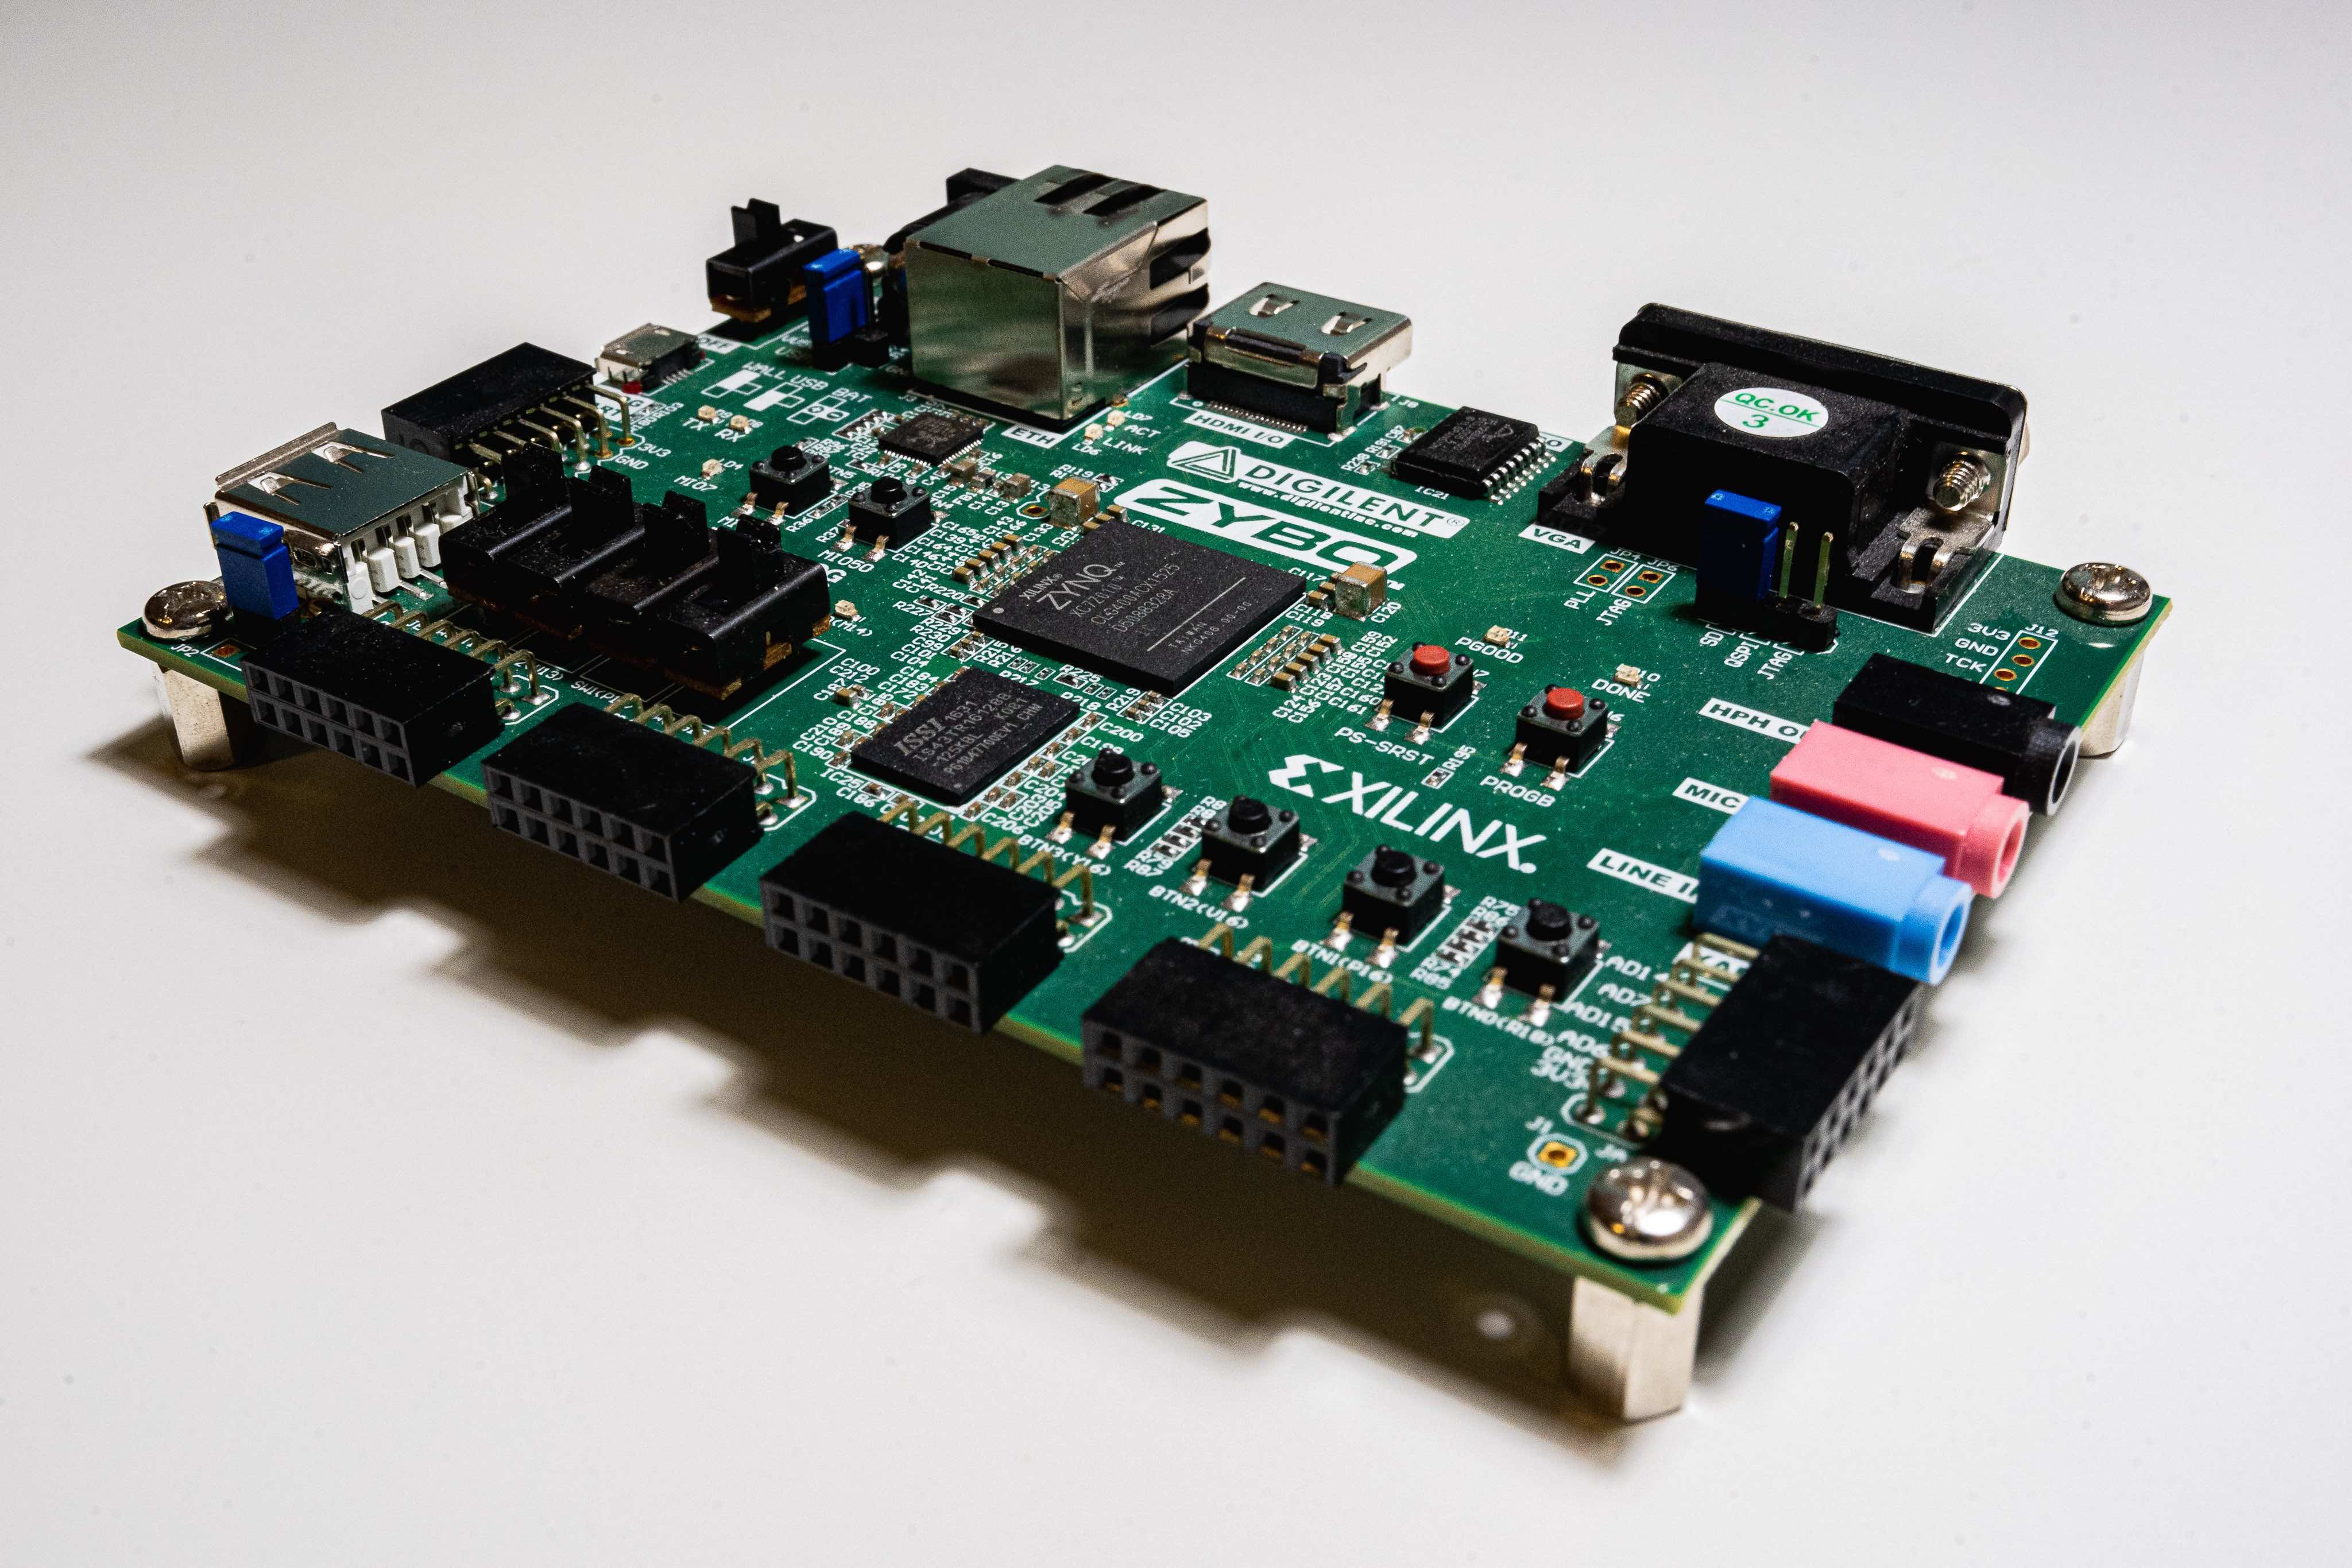
\includegraphics[width=0.85\textwidth]{src/jpg/digilent-zybo-foto-2.jpeg} 
					\caption{Vývojová deska Digilent ZYBO Zynq-7000 ARM/FPGA \gls{abbreviation:soc} Trainer Board – boční pohled.}
					\label{fig:digilent-zybo-foto-2}
			\end{figure}

		\subsection{Základní přehled}
		\subsubsection{CPU a FPGA čip}
			Hlavní částí vývojové desky je čip, obsahující \gls{abbreviation:fpga} a \gls{abbreviation:cpu} jednotky zakomponované v~jedné polovodičové struktuře. Jak již bylo zmíněno v~části \hyperref[subsec:hardware-accelerated-applications]{\textit{Hardware Accelerated Applications}}, tato struktura se nazývá heterogenní.\par
			Deska obsahuje čip Xilinx Zynq-7000 (typ XC72010), který umožňuje pro vývoj aplikací použít \gls{abbreviation:sdk} od firmy Xilinx. V~tomto čipu je integrován dvou jádrový procesor ARM Cortex-9, který slouží pro řízení akcelerovaných aplikací na Xilinx \gls{abbreviation:fpga} sedmé série. Detailní schéma blokové architektury \gls{abbreviation:soc} s~označním sběrnic a komunikace jednotlivých částí čipu je zobrazeno na obr. \ref{fig:zynq-block-diagram-detailed}.\par
			Z~naznačené architektury je možné vyvodit, že se \gls{abbreviation:soc} skládá ze dvou hlavních částí, které je možné dále rozdělit na jednotlivé bloky:
			\begin{itemize}
				\item Processing System (\gls{abbreviation:ps}),
				\begin{itemize}
					\item Application processor unit (\gls{abbreviation:apu}),
					\item Memory interfaces,
					\item \gls{abbreviation:io} peripherals (\gls{abbreviation:iop}),
					\item Interconnect,
				\end{itemize}
				\item Programmable Logic (\gls{abbreviation:pl}).
			\end{itemize}
			\vspace*{0.25cm}
			\noindent\textbf{Blok PS}\\
			Blok \gls{abbreviation:ps} se skládá z~dílčích bloků, které neslouží k~akceleraci aplikací, ale k~běhu host programu (program běžící na \gls{abbreviation:ps}). Blok \gls{abbreviation:ps} reprezentuje prakticky celou architekturu čipu vyjma části věnované \gls{abbreviation:pl}.\par\vspace*{0.25cm}
			\noindent\textbf{Blok APU}\\
			Blok \gls{abbreviation:apu} obsahuje \gls{abbreviation:cpu} Cortex-A9 a další podpůrné bloky jako např. přímý přístup do paměti (\gls{abbreviation:dma} controller), General interrupt controller (\gls{abbreviation:gic}) pro maskování a ovládání přerušení, watchdog a další podpůrné bloky.\par\vspace*{0.25cm}
			\noindent\textbf{Blok Memory interfaces}\\
			Memory interfaces slouží k~přístupu \gls{abbreviation:apu} a \gls{abbreviation:pl} k~pamětím typu DDR3, DDR3L, DDR2 a LPDDR-2. Je možné také vybrat, zda šířka sběrnice bude 16, nebo 32 bitů. K~dispozici jsou zakomponované kotroléry přenosu dat pro optimalizaci rychlosti, Static Memory Controller nebo Quad-\gls{abbreviation:spi} Controller.\par\vspace*{0.25cm}
			\noindent\textbf{Blok IOP}\\
			IOP se skládá ze standardizovaných rozhraní vhodných pro průmyslovou komunikaci. Obsahuje např. \gls{abbreviation:gpio}, Gigabit Ethernet, dva bloky \gls{abbreviation:usb} Controller, dva bloky \gls{abbreviation:sd}/SDIO Controller pro bootování \gls{abbreviation:sd} karty, dva bloky \gls{abbreviation:spi} Controller, dva bloky \gls{abbreviation:can} Controller, dva bloky \gls{abbreviation:uart} Controller a dva bloky \gls{abbreviation:iic} Controller.\par\vspace*{0.25cm}
			\noindent\textbf{Blok Interconnect}\\
			Blok Interconnect, resp. na obr. \ref{fig:zynq-block-diagram-detailed} označený Central Interconnect slouží k~propojení jednotlivých bloků \gls{abbreviation:soc} dle požadované technologie a rychlosti.\par\vspace*{0.25cm}
			\noindent\textbf{Blok PL}\\
			Blok \gls{abbreviation:pl} reprezentuje logické programovatelné pole (\gls{abbreviation:fpga}), v~němž jsou zakomponovány další podpůrné prvky jako např. blok zpracování digitálních signálů, řízení taktovacích hodin, analogově digitální převodník (\gls{abbreviation:adc}).\par\vspace*{0.35cm}
			\noindent Detailní technické specifikace, složení a parametry jmenovaných bloků jsou uvedeny v~\cite{xilinx-zynq-7000-technical-reference-manual}.
			% \begin{figure}[htbp!]
			% 	\centering
			% 		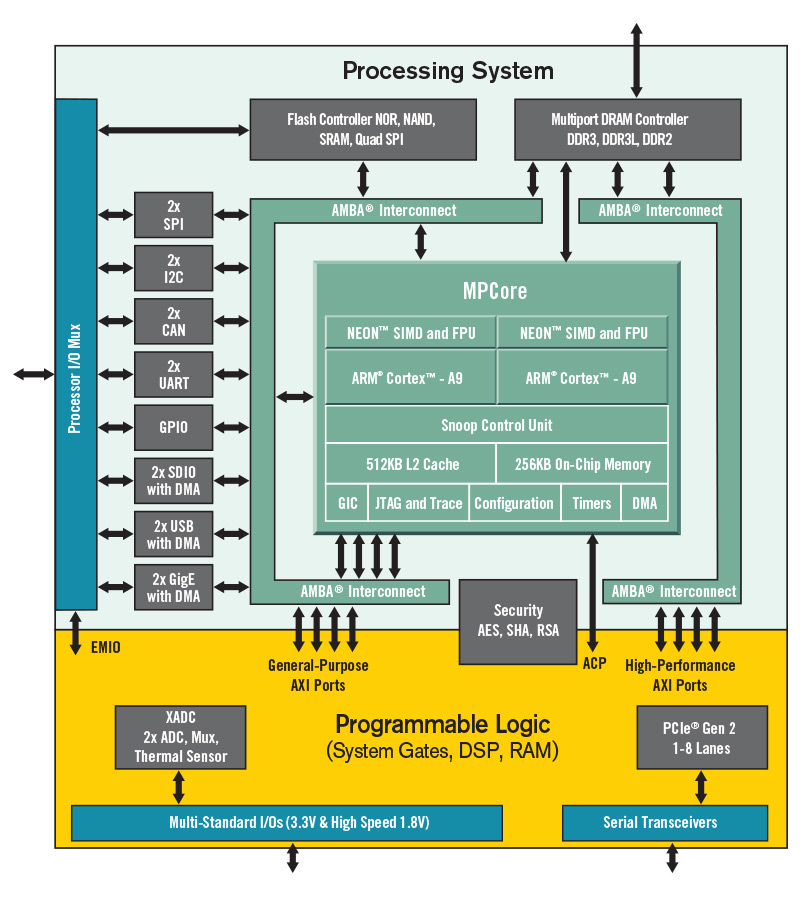
\includegraphics[width=0.75\textwidth]{src/png/zynq-mp-core-dual.png} 
			% 		\caption{Blokové schéma čipu Zynq-7000, umístěného na vývojové desce \textit{Digilent ZYBO Zynq-7000 ARM/FPGA SoC Trainer Board}. (převzato z \cite{xilinx-zynq-7000-socs-with-hardware-and-software-programmability})}
			% 		\label{fig:zynq-mp-core-dual}
			% \end{figure}

			\begin{figure}[htbp!]
				\centering
					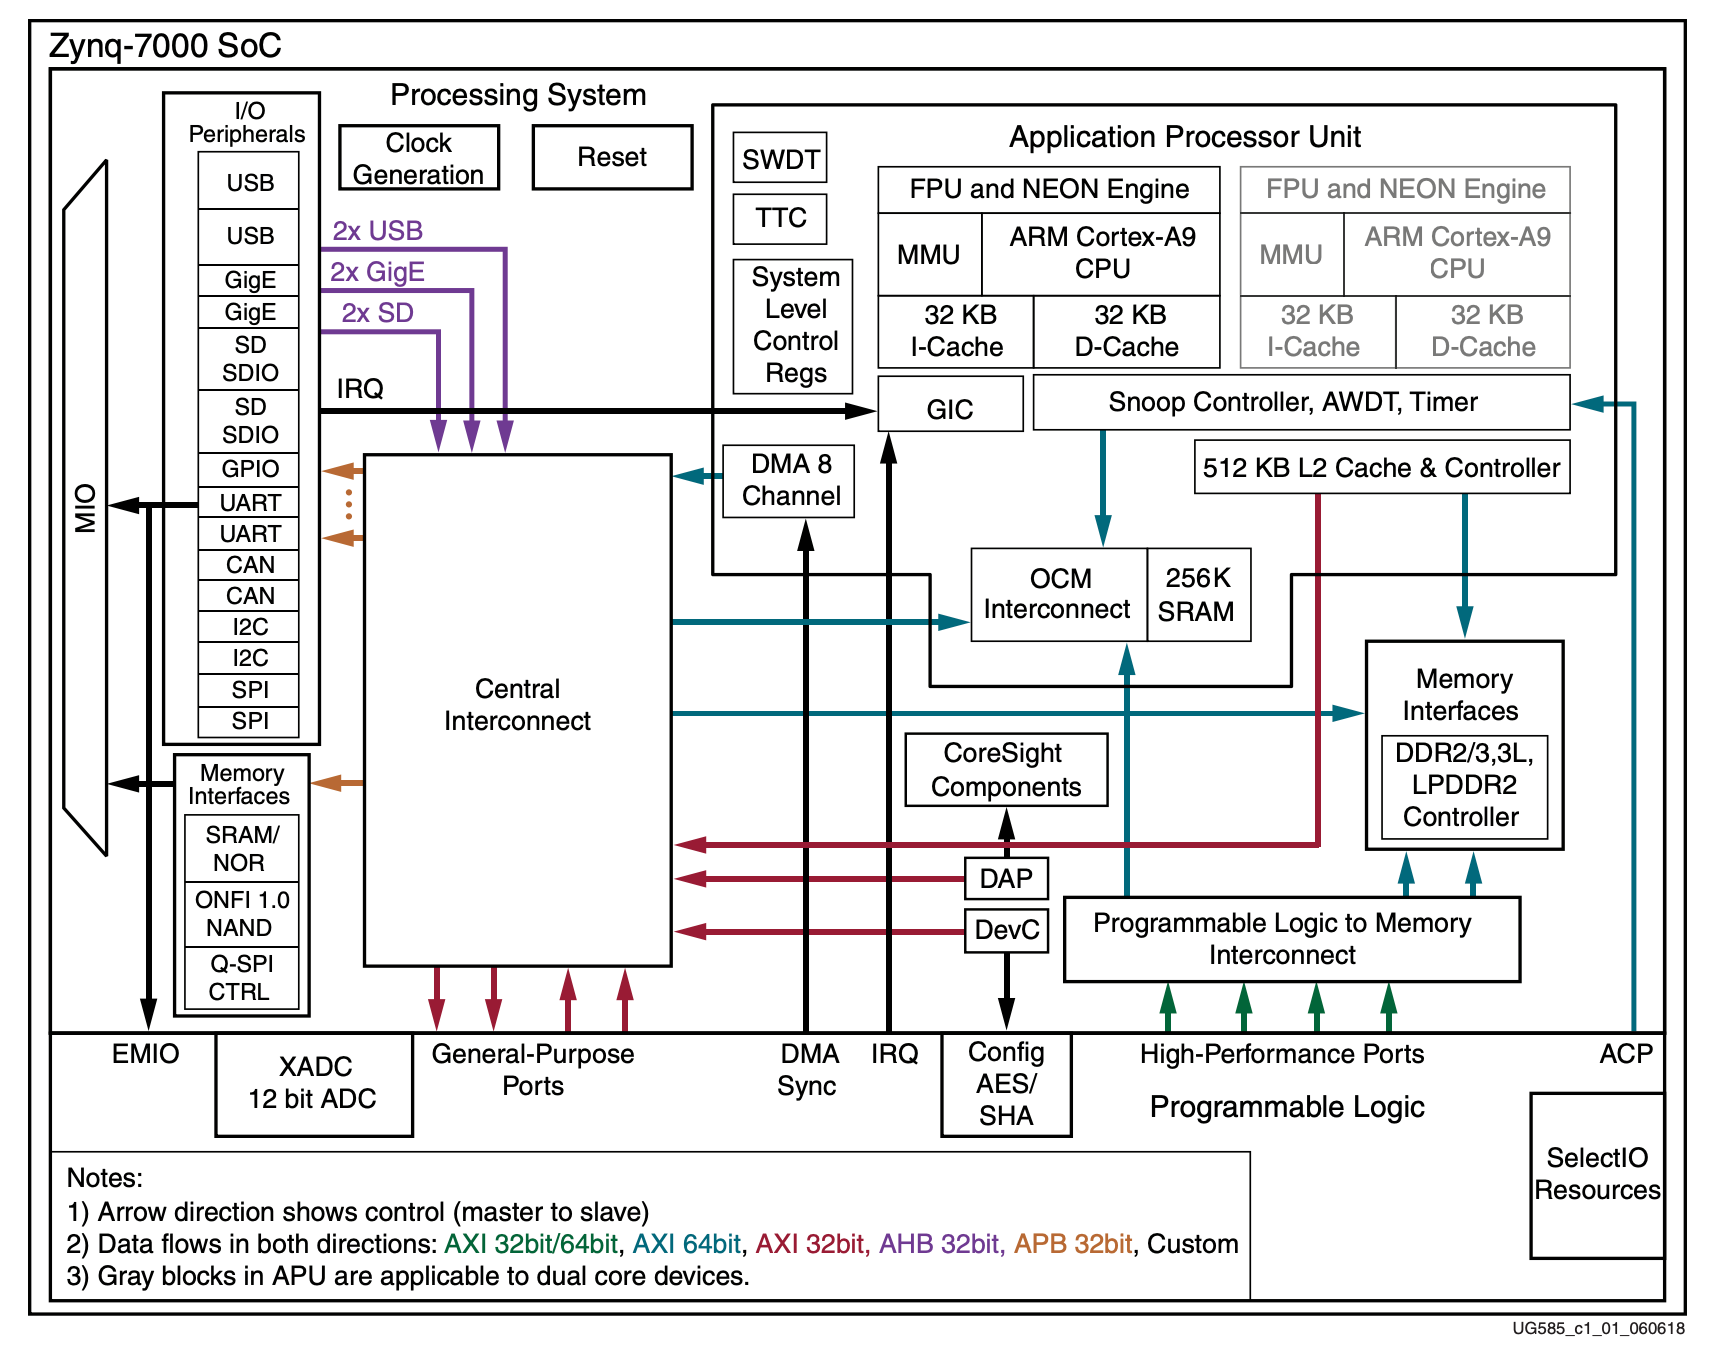
\includegraphics[width=0.75\textwidth]{src/png/zynq-block-diagram-detailed.png} 
					\caption{Detailní schéma čipu Zynq-7000, umístěného na vývojové desce \textit{Digilent ZYBO Zynq-7000 ARM/FPGA SoC Trainer Board}. (převzato z~\cite{xilinx-zynq-7000-technical-reference-manual})}
					\label{fig:zynq-block-diagram-detailed}
			\end{figure}
			\fbar
			\subsubsection{Uspořádání vývojové desky Zybo Zynq-7000}
				Na obr. \ref{fig:digilent-zybo-foto-1-oznacene} je zobrazen horní pohled na vývojovou desku, na kterém jsou vyznačeny významné části, jimž je vhodné věnovat pozornost. Číselné označení koresponduje s~označením a vysvětlivkou v~tabulce \ref{tab:digilent-zybo-zynq-7000-description}. Pro úplnost je spodní strana desky zobrazena na obr. \ref{fig:digilent-zybo-foto-3}.

				\begin{figure}[H]
					\centering
						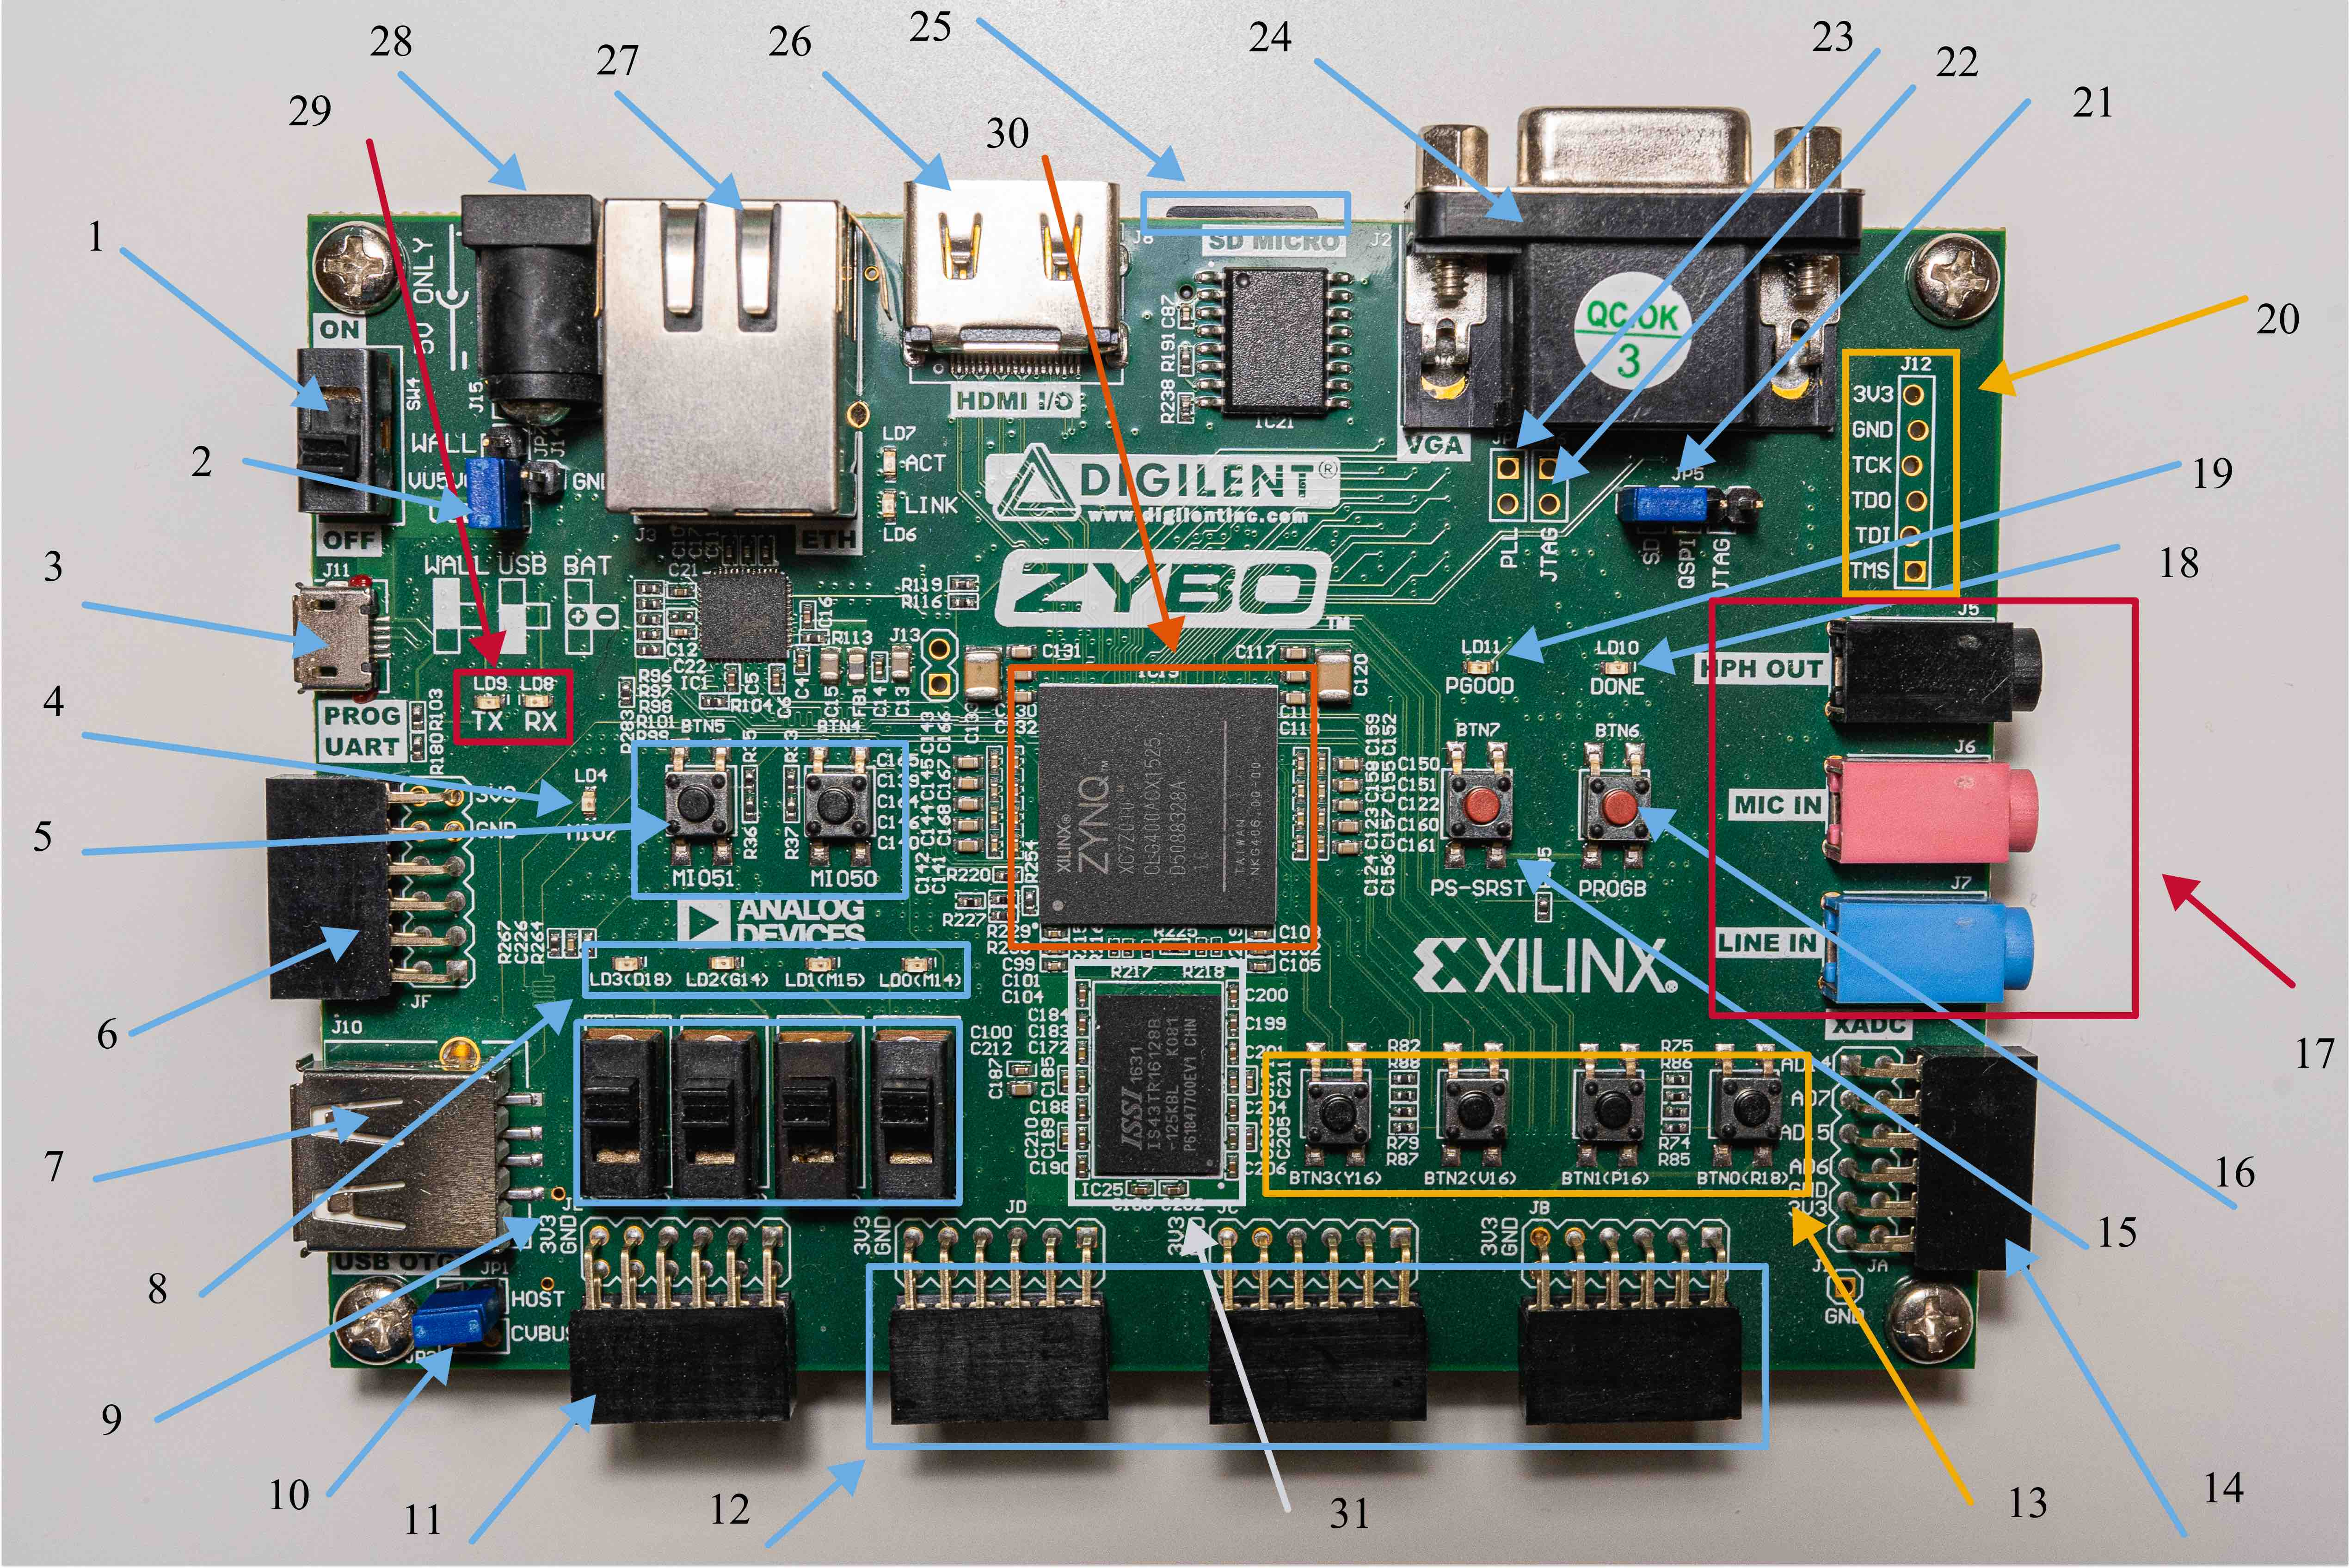
\includegraphics[width=0.85\textwidth]{src/jpg/digilent-zybo-foto-1-oznacene.jpeg} 
						\caption{Vývojová deska Digilent ZYBO Zynq-7000 ARM/FPGA SoC Trainer Board – vrchní pohled s~vyznačením komponent.}
						\label{fig:digilent-zybo-foto-1-oznacene}
				\end{figure}

				\begin{figure}[H]
					\centering
						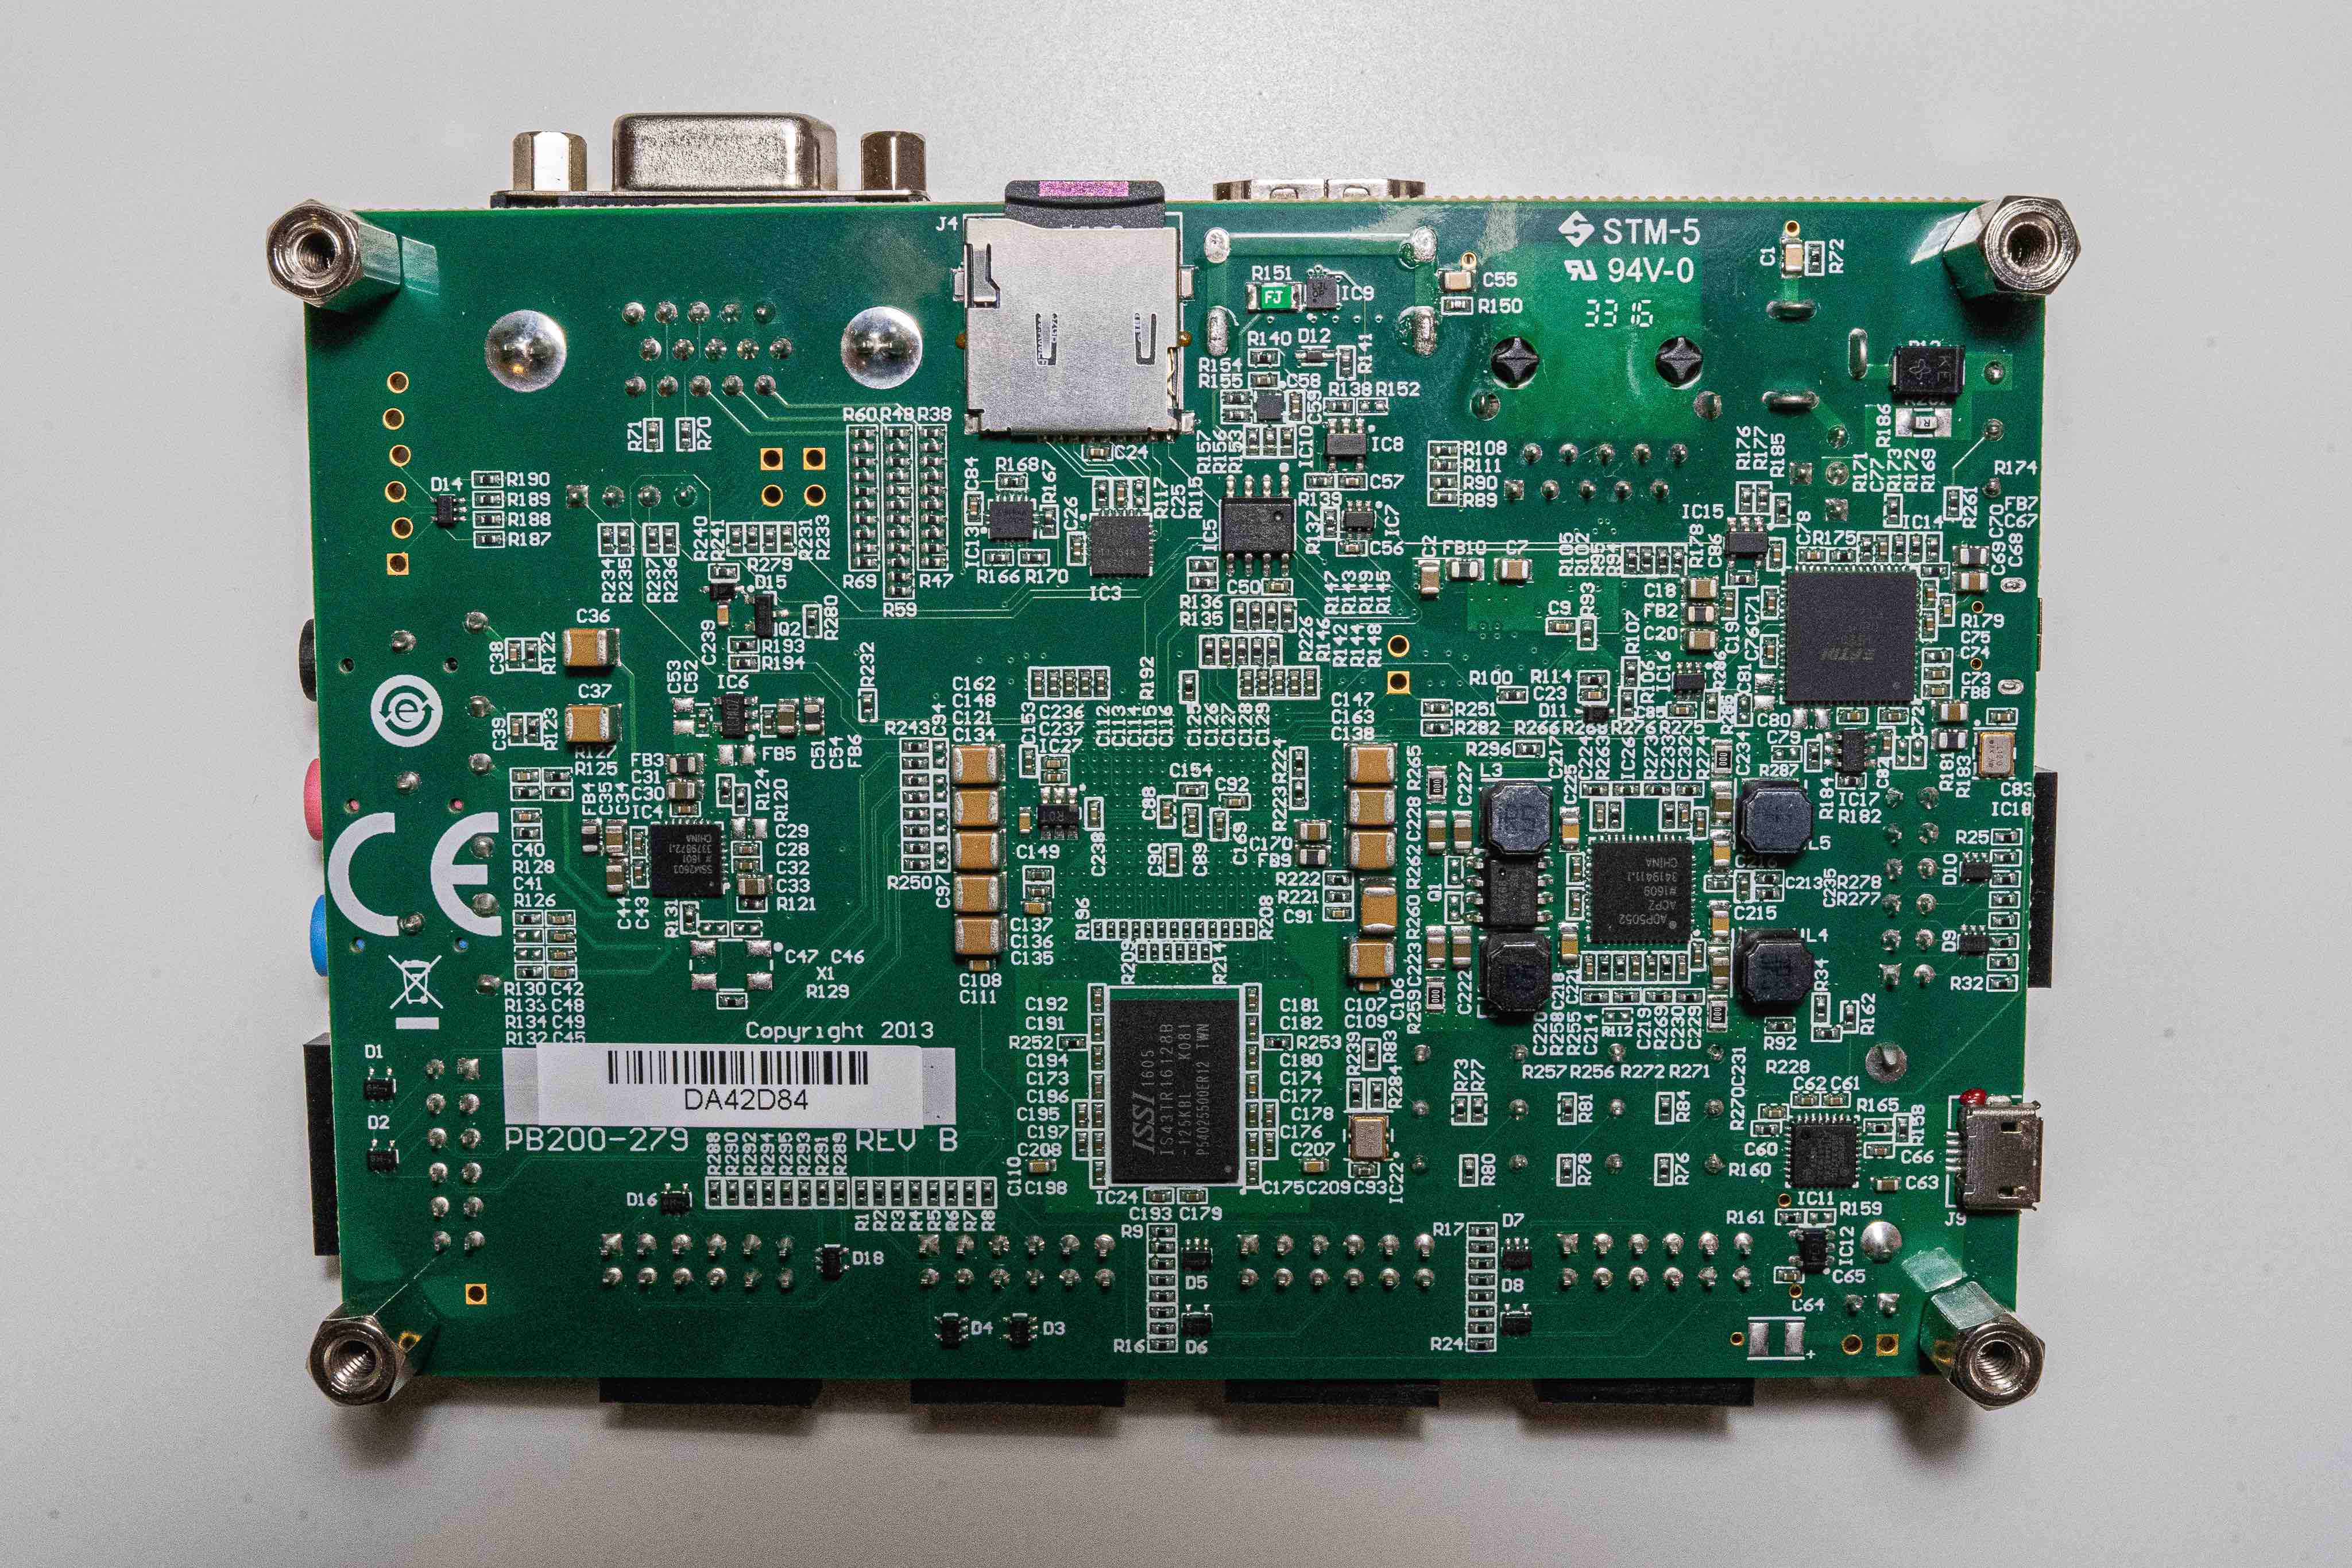
\includegraphics[width=0.85\textwidth]{src/jpg/digilent-zybo-foto-3.jpeg} 
						\caption{Vývojová deska Digilent ZYBO Zynq-7000 ARM/FPGA SoC Trainer Board – spodní pohled.}
						\label{fig:digilent-zybo-foto-3}
				\end{figure}

			\fbar
			\begin{table}[htbp!]
				\centering
				\caption{Popis označených komponent na vývojové desce Digilent Zybo Zynq-7000. (informace a značení převzaty z~\cite{digilent-zybo-reference-manual})}
			  \vspace*{0.15cm}
			   \resizebox{\textwidth}{!}
				{
				\begin{tabular}{!{\vrule width 2pt} c | l | l !{\vrule width 2pt}}\noalign{\hrule height 2pt}
				\rowcolor{codeblue}
				označení & popis &	poznámka \\
				\noalign{\hrule height 2pt}
				1 & Power Switch & galvanické sepnutí napájecího obvodu \\ \hline
				2 & Power Select Jumper and Battery Header & výběr napájecího vstupu konektor, \gls{abbreviation:usb}, baterie\\ \hline
				3 & Shared \gls{abbreviation:uart}/\gls{abbreviation:jtag} \gls{abbreviation:usb} port & komunikace \gls{abbreviation:uart} a \gls{abbreviation:jtag} debugging\\ \hline
				4 & MIO \gls{abbreviation:led} & multiplexed \gls{abbreviation:led} – možnost výběru signálu\\ \hline
				5 & MIO Pushbuttons (2) & multiplexed input\\ \hline
				6 & MIO Pmod & možnost připojení periférií\\ \hline
				7 & \gls{abbreviation:usb} OTG Connectors & \gls{abbreviation:usb} port typ A/micro \gls{abbreviation:usb} (spodní část)\\ \hline
				8 & Logic \gls{abbreviation:led}s (4) & zobrazování 1/0\\ \hline
				9 & Logic Slide Switches (4) & logický vstup 1/0\\ \hline
				10 & \gls{abbreviation:usb} OTG Host/Device Select Jumpers & výběr módu zařízení\\ \hline
				11 & Standard \gls{abbreviation:pmod} & chráněné \gls{abbreviation:pmod}, limitace max. přenosu informace\\ \hline
				12 & High-speed \gls{abbreviation:pmod}s (3) & jako standard ale bez ochrany, vyšší rychlost\\ \hline
				13 & Logic Pushbuttons (4) & logický vstup 1/0\\ \hline
				14 & XADC \gls{abbreviation:pmod} & možnost  analog/digi input/output, spojeno s~\gls{abbreviation:adc} v~Zynq\\ \hline
				15 & Processor Reset Pushbutton & reset \gls{abbreviation:pl}, paměti v~\gls{abbreviation:ps}\\ \hline
				16 & Logic Configuration reset Pushbutton & reset \gls{abbreviation:pl}, zrušení DONE informace\\ \hline
				17 & Audio Codec Connectors & stereo line in, mono mikrofon, stereo output\\ \hline
				18 & Logic Configuration Done \gls{abbreviation:led} & signál o~úspěšném dokončení konfigurace PL\\ \hline
				19 & Board Power Good \gls{abbreviation:led} & 1/0, 1 – nominální napětí na všech sběrnicích\\ \hline
				20 & \gls{abbreviation:jtag} Port for optional external cable & externí \gls{abbreviation:jtag}\\ \hline
				21 & Programming Mode Jumper & výběr „programovacího vstupu“, \gls{abbreviation:sd} karta, \gls{abbreviation:qspi}, \gls{abbreviation:jtag}\\ \hline
				22 & Independent \gls{abbreviation:jtag} Mode Enable Jumper & \gls{abbreviation:jtag} mimo \gls{abbreviation:ps}, viditelné pouze \gls{abbreviation:pl}\\ \hline
				23 & PLL Bypass Jumper & přemostění PLL (\gls{abbreviation:clk}), pro možnost konfigurace PLL\\ \hline
				24 & VGA connector & připojení displeje\\ \hline
				25 & microSD connector & na spodní straně\\ \hline
				26 & HDMI Sink/Source Connector & input/ouput, nutné implementovat encoding a decoding v~logice\\ \hline
				27 & Ethernet RJ45 Connector & komunikace\\ \hline
				28 & Power Jack & napájení 5 V/2,5 A\\ \hline
				29 & TX/RX \gls{abbreviation:led} & indikace \gls{abbreviation:uart} komunikace\\ \hline
				30 & Xilinx Zynq \gls{abbreviation:soc} & systém na čipu\\ \hline
				31 & DDR2 Memory & \gls{abbreviation:ram}\\\noalign{\hrule height 2pt}
				\end{tabular}
				}
				\label{tab:digilent-zybo-zynq-7000-description}
			\end{table}


			

		\fbar
		\section{Vývojová deska Xilinx Kria KR260}
				Deska od firmy Digilent, představená v~části \hyperref[sec:vyvojova-deska-digilent-zybo]{\textit{Vývojová deska Digilent Zybo}}, je vhodná pouze pro prvotní seznámení s~procesem~vytváření akcelerovaných aplikací. Pro náročnější aplikace, které vyžadují využití většího množství \gls{abbreviation:luts}, nebylo v~této práci možné Zybo použít. Naopak \gls{abbreviation:pl} vývojové desky Kria KR260 obsahuje dostatečné množství \gls{abbreviation:luts} a díky svým moderním komponentám, může být efektivně využita k~tvorbě náročnějších aplikací.\par
				Hlavní částí vývojové desky KR260 je „modul“ \textit{Kria K26 System-on-Module}. Tudíž oproti Digilent Zybo, které využívá \gls{abbreviation:soc}, deska KR260 využívá \gls{abbreviation:som}. Přednosti jednotlivých architektur byly již představeny v~části \hyperref[sec:system-on-a-chip]{\textit{System on a chip}} a \hyperref[sec:system-on-modules]{\textit{System on modules}}. Po ukončení vývoje aplikace na vývojové desce (a popřípadě po ukončení vytváření návrhu \gls{abbreviation:cc}) je možné pro aplikaci v~průmyslu zakoupit samostatný modul na \gls{abbreviation:bb} ve vhodné variantě, a umístit ho na danou \gls{abbreviation:cc}. V~této práci je využíván standardní vývojový „Starter kit“ s~deskou KR260, jejíž komponenty je vhodné představit.

				\begin{figure}[H]
					\centering
						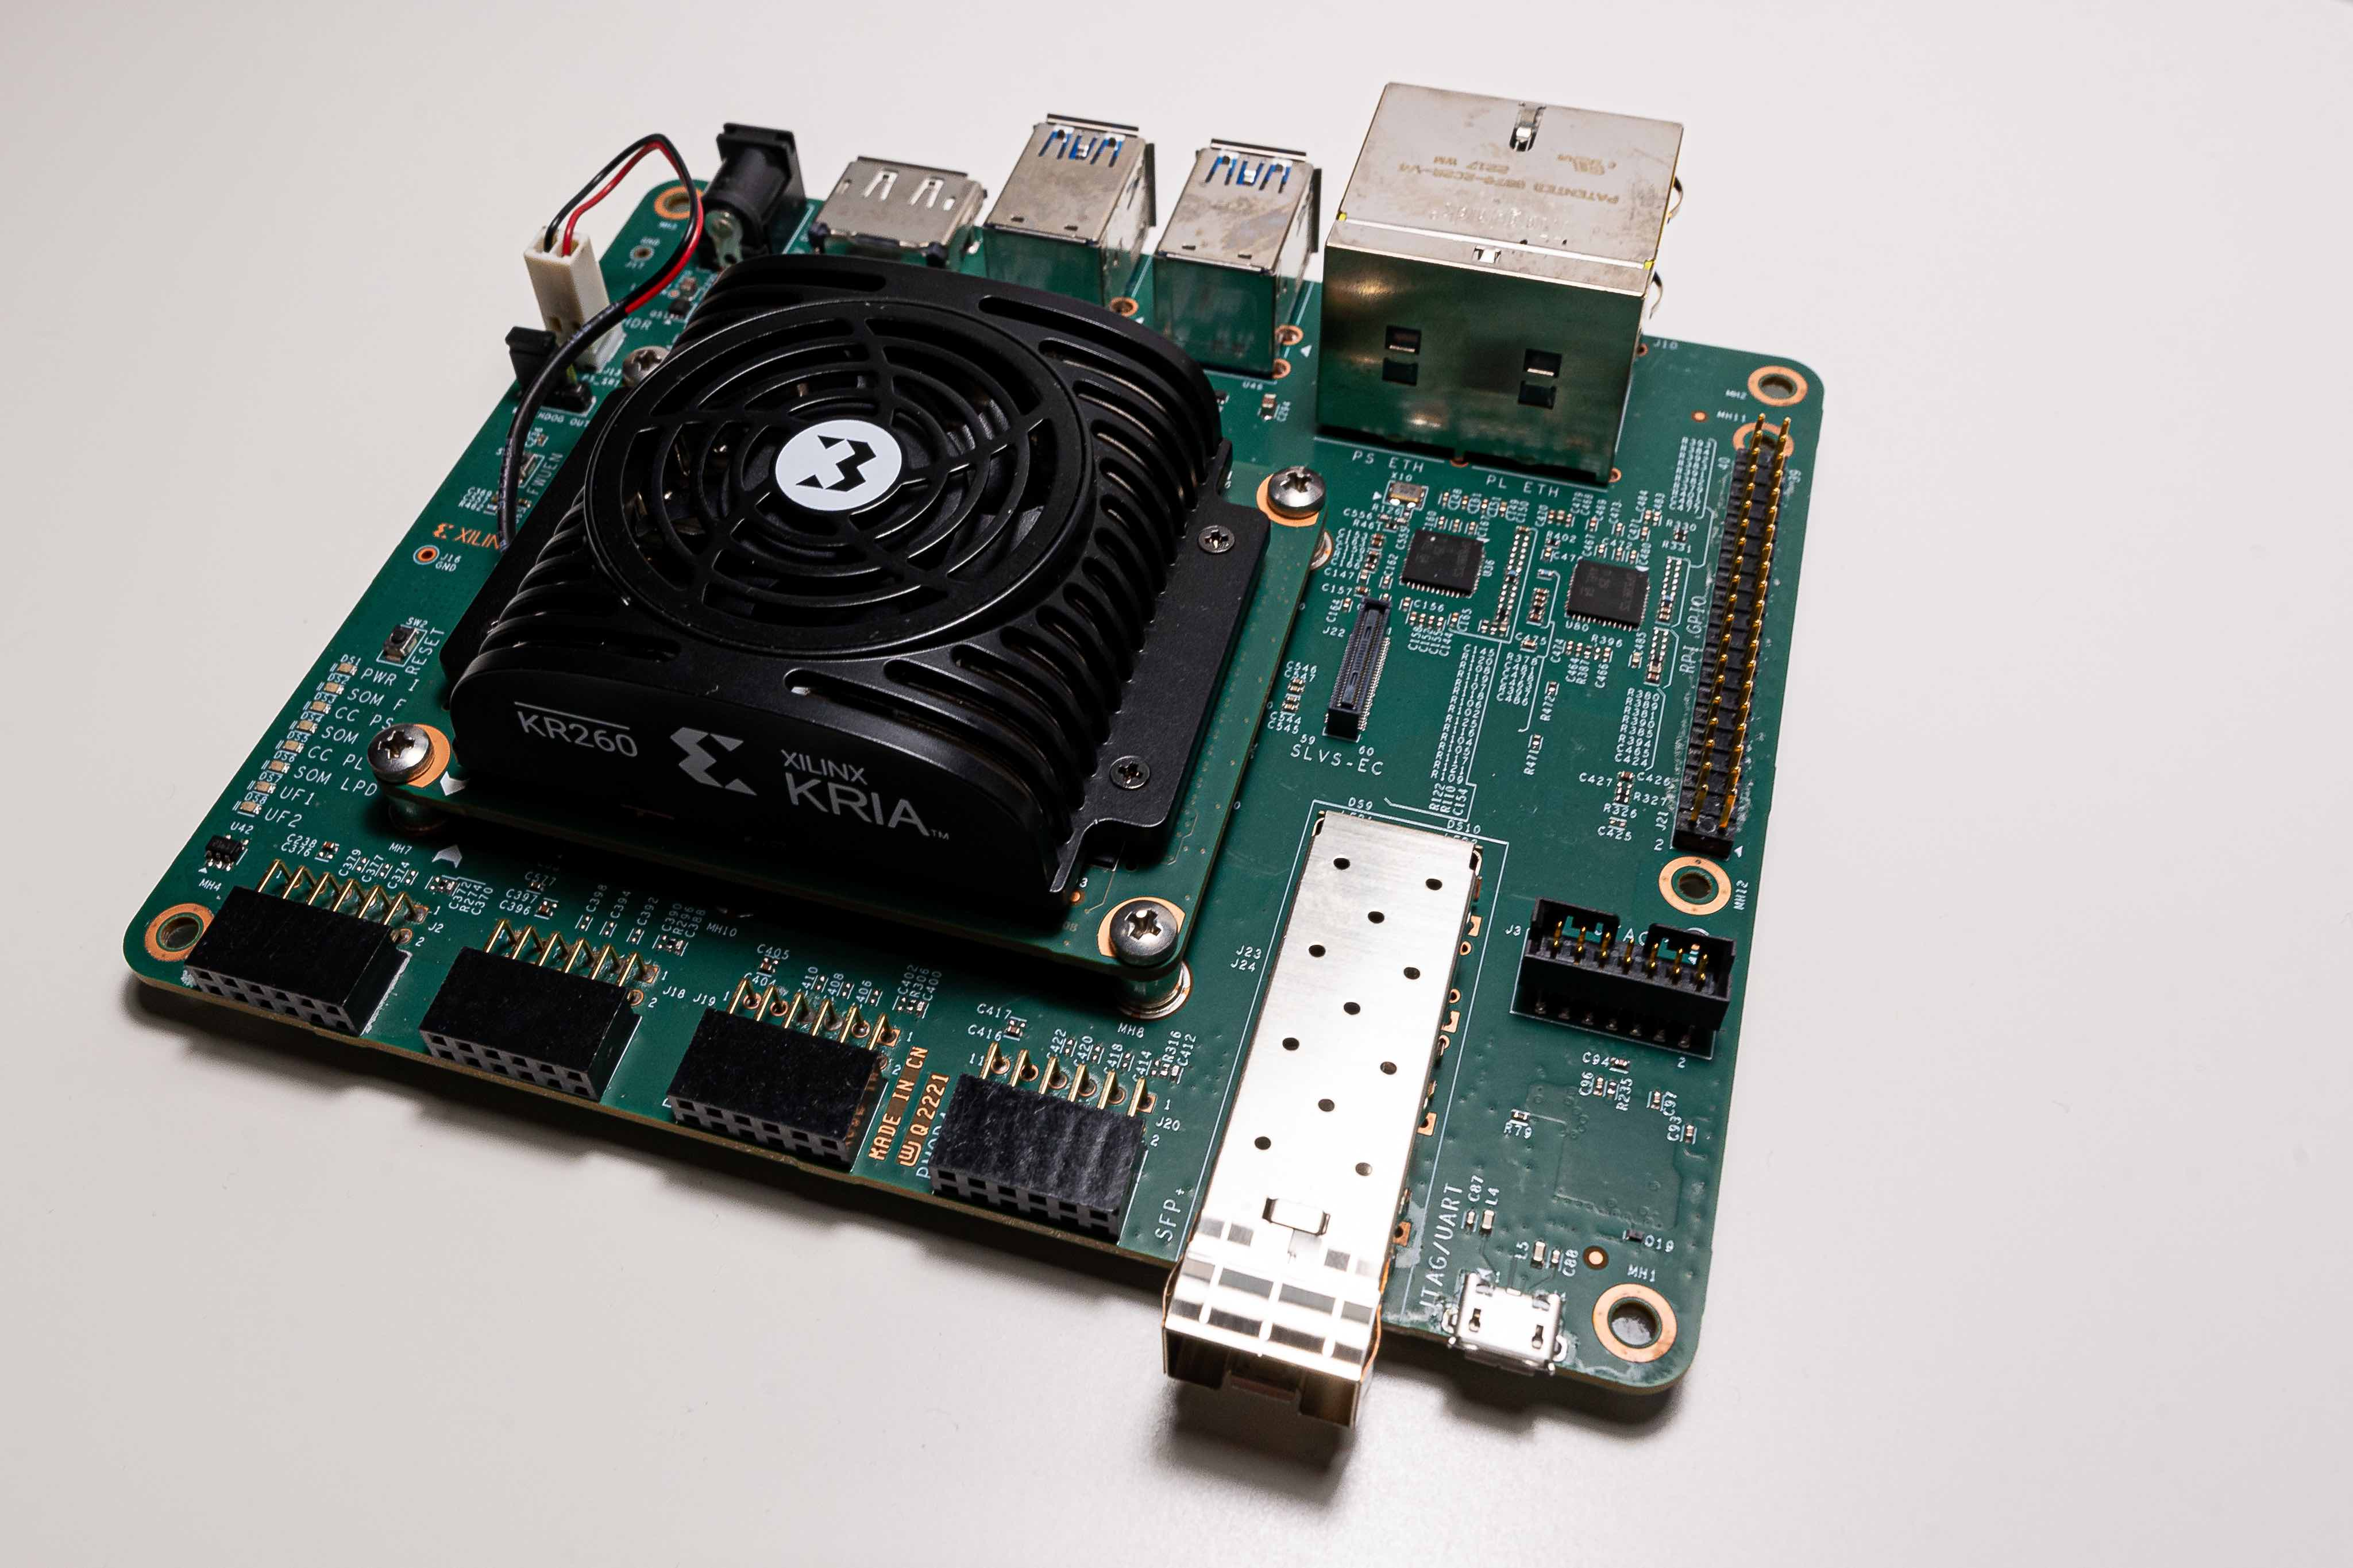
\includegraphics[width=0.85\textwidth]{src/jpg/xilinx-kria-foto-1.jpeg} 
						\caption{Vývojová deska Xilinx Kria KR260 – boční pohled.}
						\label{fig:xilinx-kria-foto-1}
				\end{figure}

				\subsection{Základní přehled}
					\subsubsection{CPU a FPGA čip}
						Strukturu \gls{abbreviation:som} je možné popsat jako modernější a komplexnější. Základní struktura obsahuje bloky \gls{abbreviation:ps} a \gls{abbreviation:pl}. Ukázkový blokový diagram struktury udávané výrobcem je na obr. \ref{fig:xilinx-kria-k26-block-diagram}.\par
						Největšími rozdíly mezi použitými \gls{abbreviation:soc} Zybo a \gls{abbreviation:som} Kria je např. velikost operační paměti, počet jader, taktovací frekvence procesorů v~\gls{abbreviation:ps}, počet \gls{abbreviation:luts} nebo logických buněk v~\gls{abbreviation:fpga} (\gls{abbreviation:pl}). Úplné specifikace pro K26 \gls{abbreviation:som} je možné nalézt v~\cite{kria-k26-som-ds}.

						\begin{figure}[htbp!]
							\centering
								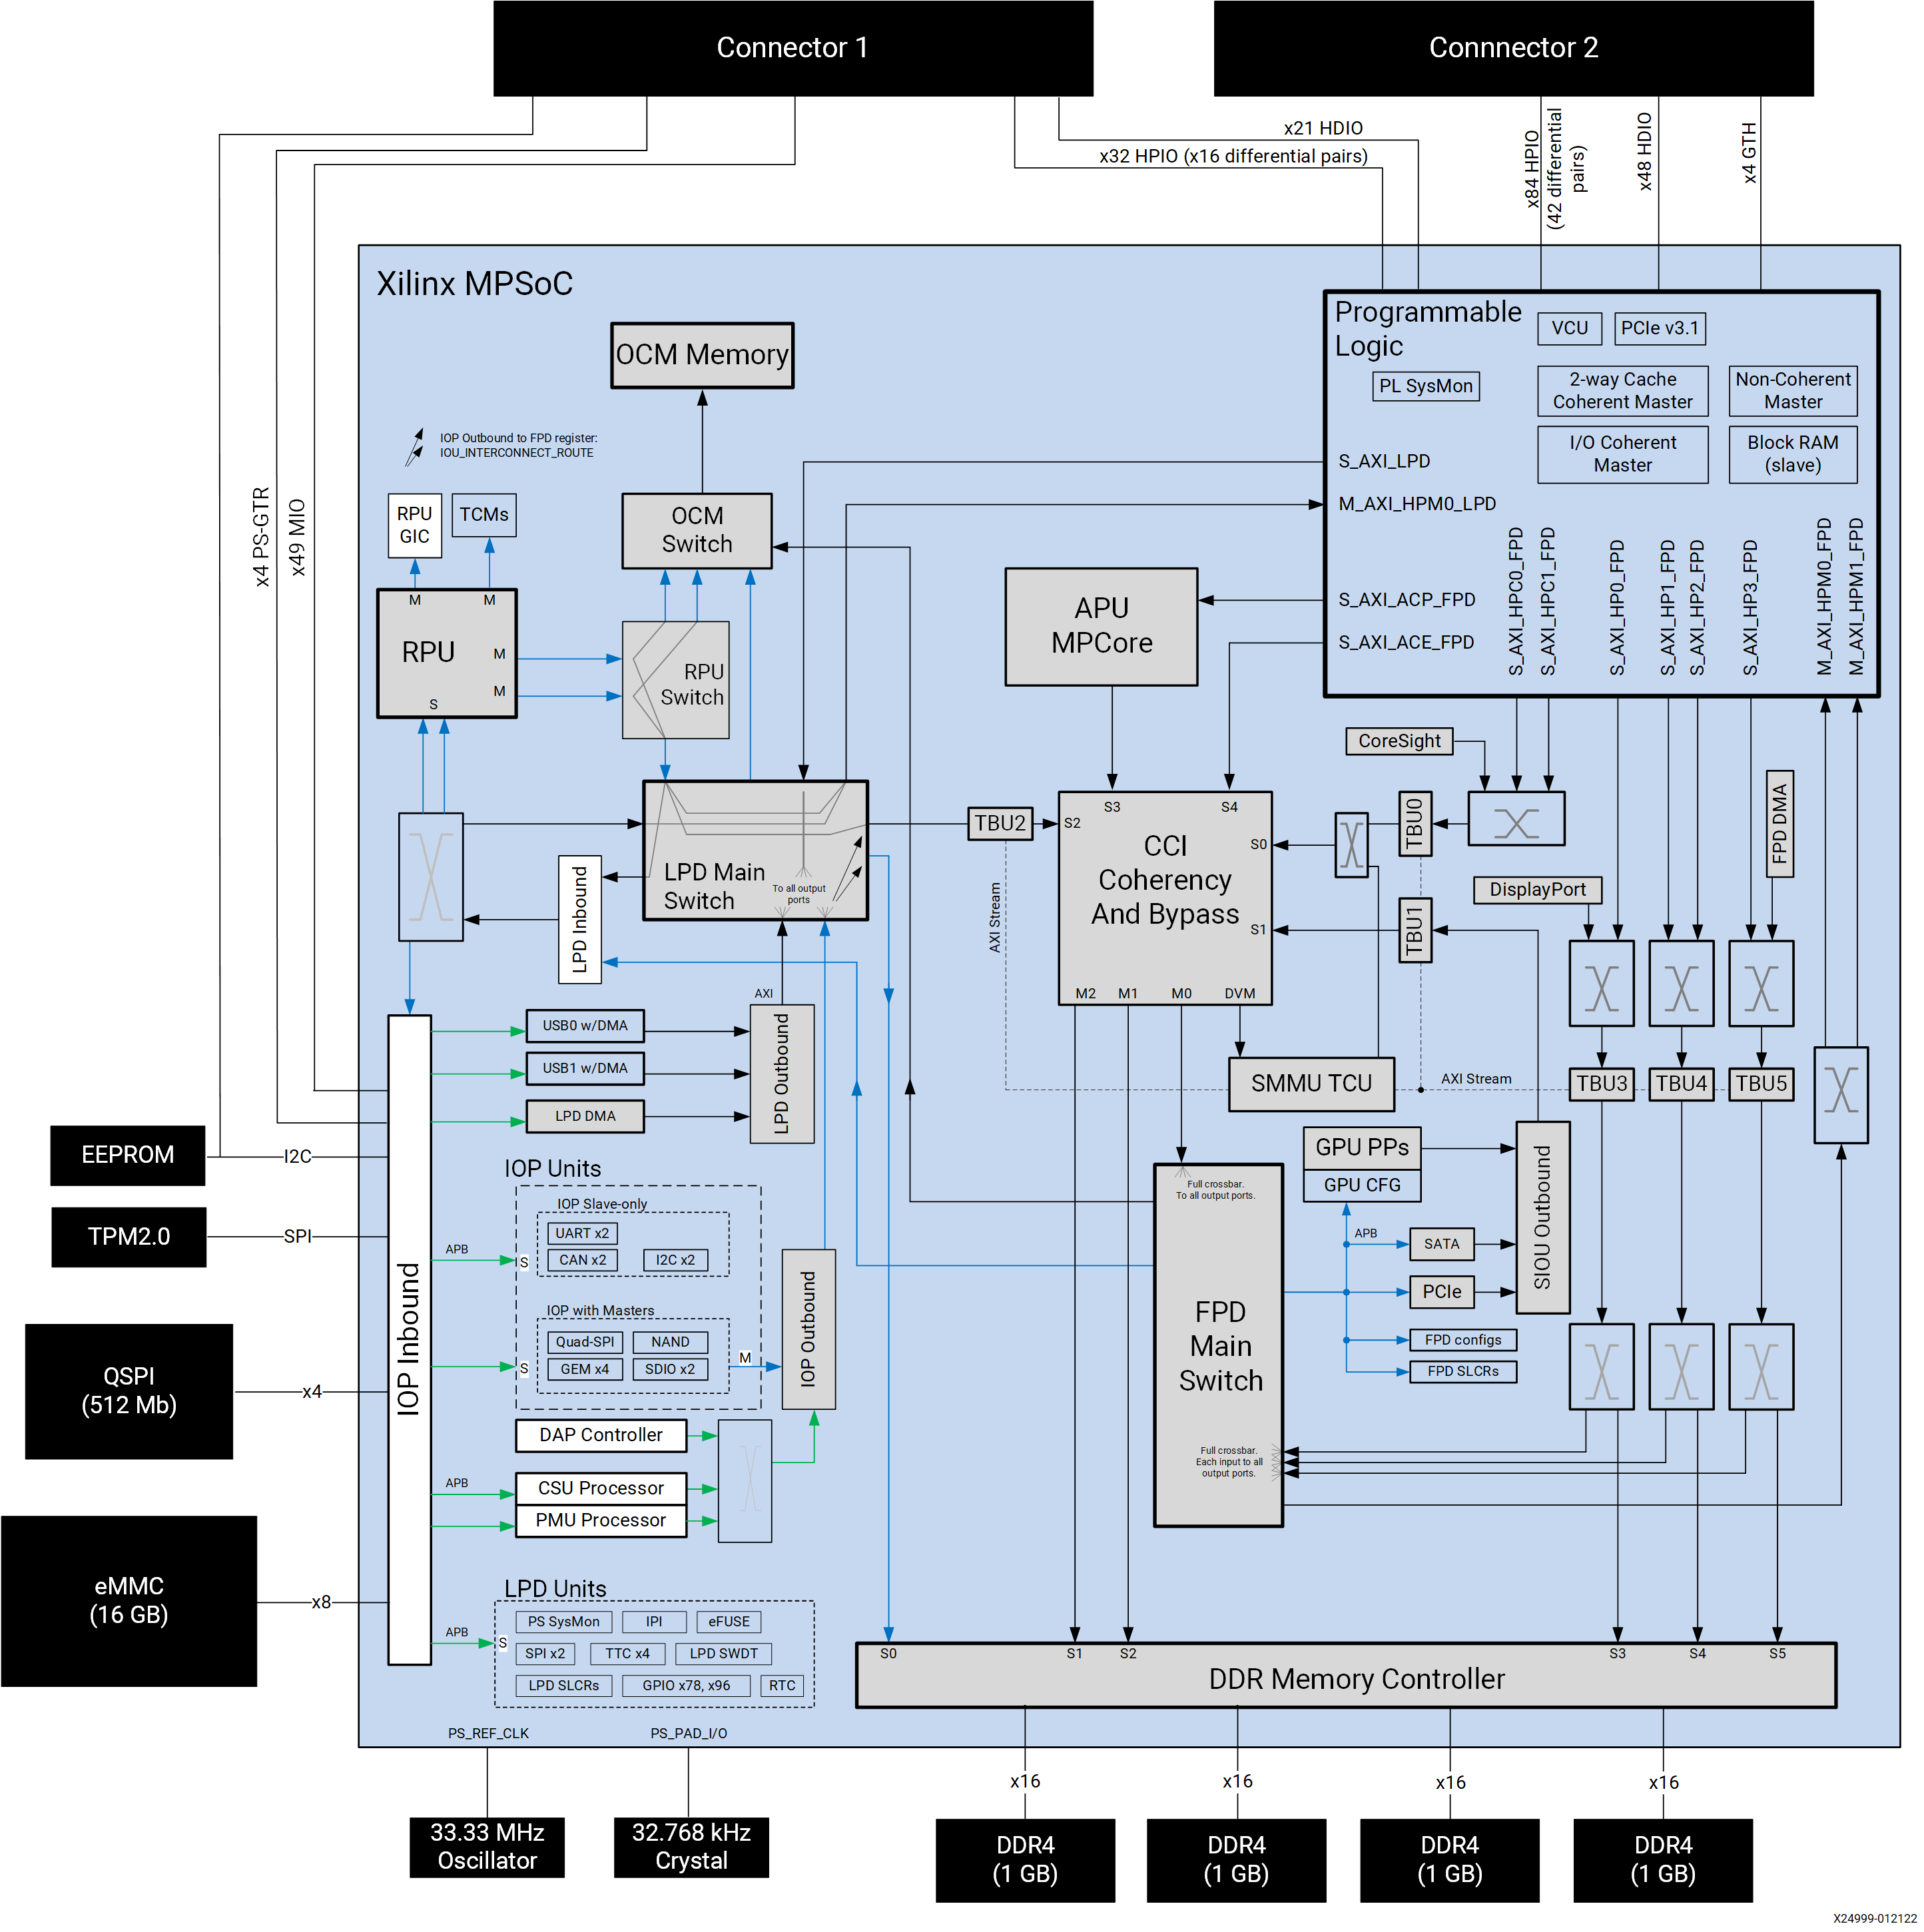
\includegraphics[width=0.95\textwidth]{src/jpg/xilinx-kria-k26-block-diagram.jpg} 
								\caption{Blokový diagram K26 \gls{abbreviation:som} Kria. \cite{kria-k26-som-ds}}
								\label{fig:xilinx-kria-k26-block-diagram}
						\end{figure}
						\fbar


				\subsection{Uspořádání vývojové desky}
				Na obr. \ref{fig:xilinx-kria-foto-2-oznacene} je zobrazen horní pohled na vývojovou desku, na kterém jsou vyznačeny významné části, jimž je vhodné věnovat pozornost. Číselné označení koresponduje s~označením a vysvětlivkou v~tabulce \ref{tab:xilinx-kria-description}. Na spodní straně desky je umístěn slot pro \gls{abbreviation:sd} kartu, na kterou je umisťován (flashován) operační systém pro \gls{abbreviation:ps}. Pro úplnost je spodní strana desky zobrazena na obr. \ref{fig:xilinx-kria-foto-3}.
				\fbar
				\begin{table}[htbp!]
					\centering
					\caption{Popis označených komponent na vývojové desce  Xilinx Kria KR260. (informace a značení převzaty z~\cite{kria-kr260-robotics-starter-kit-user-guide})}
			  		\vspace*{0.15cm}
			   		\resizebox{\textwidth}{!}
						{
							\begin{tabular}{!{\vrule width 2pt} c | l | l !{\vrule width 2pt}}\noalign{\hrule height 2pt}
							\rowcolor{codeblue}
							označení & popis &	poznámka \\
							\noalign{\hrule height 2pt}
							1 & \gls{abbreviation:som} modul na \gls{abbreviation:bb} a Fansink & -  \\ \hline
							2 & J13 Fan Power & napájení větráku chladiče  \\ \hline
							3 & J1 watchdog & -  \\ \hline
							4 & \gls{abbreviation:switch}1 Firmware Update & -  \\ \hline
							5 & \gls{abbreviation:switch}2 Reset & -  \\ \hline
							6 & DS1–DS6 Power Status \gls{abbreviation:led}s & pokud vše ok, zbarveny zeleně  \\ \hline
							7 & DS7–DS8 (UF1 a UF2) Uživatelsky ovládané \gls{abbreviation:led} & -  \\ \hline
							8 & J2, J18, J19, J20 \gls{abbreviation:pmod} konektory & -  \\ \hline
							9 & J23 a J24 SFP+ & optický konektor  \\ \hline
							10 & J4 Micro \gls{abbreviation:usb} & UART/JTAG  \\ \hline
							11 & J3 PC4 JTAG & -  \\ \hline
							12 & J22 SLVS-EC & konektor pro připojení kamery  \\ \hline
							13 & DS36 Raspberry Pi HAT & -  \\ \hline
							14 & J10A, J10B RJ-45 \gls{abbreviation:pl} Ethernet & konektor připojen přes \gls{abbreviation:ps}  \\ \hline
							15 & J10C, J10D RJ-45 PS Ethernet & konektor připojen do \gls{abbreviation:ps}  \\ \hline
							16 & U46 \gls{abbreviation:usb}3.0 & -  \\ \hline
							17 & U44 \gls{abbreviation:usb}3.0 & -  \\ \hline
							18 & DS36 \gls{abbreviation:ps} Status \gls{abbreviation:led} & -  \\ \hline
							19 & DS35 HeartBeat \gls{abbreviation:led} & -  \\ \hline
							20 & DS34 \gls{abbreviation:ps} Done LED & -  \\ \hline
							21 & J6 DisplayPort & -  \\ \hline
							22 & J12 \gls{abbreviation:dc} Jack & -\\\noalign{\hrule height 2pt}
							\end{tabular}
						}
					\label{tab:xilinx-kria-description}
				\end{table}

				\begin{figure}[H]
					\centering
						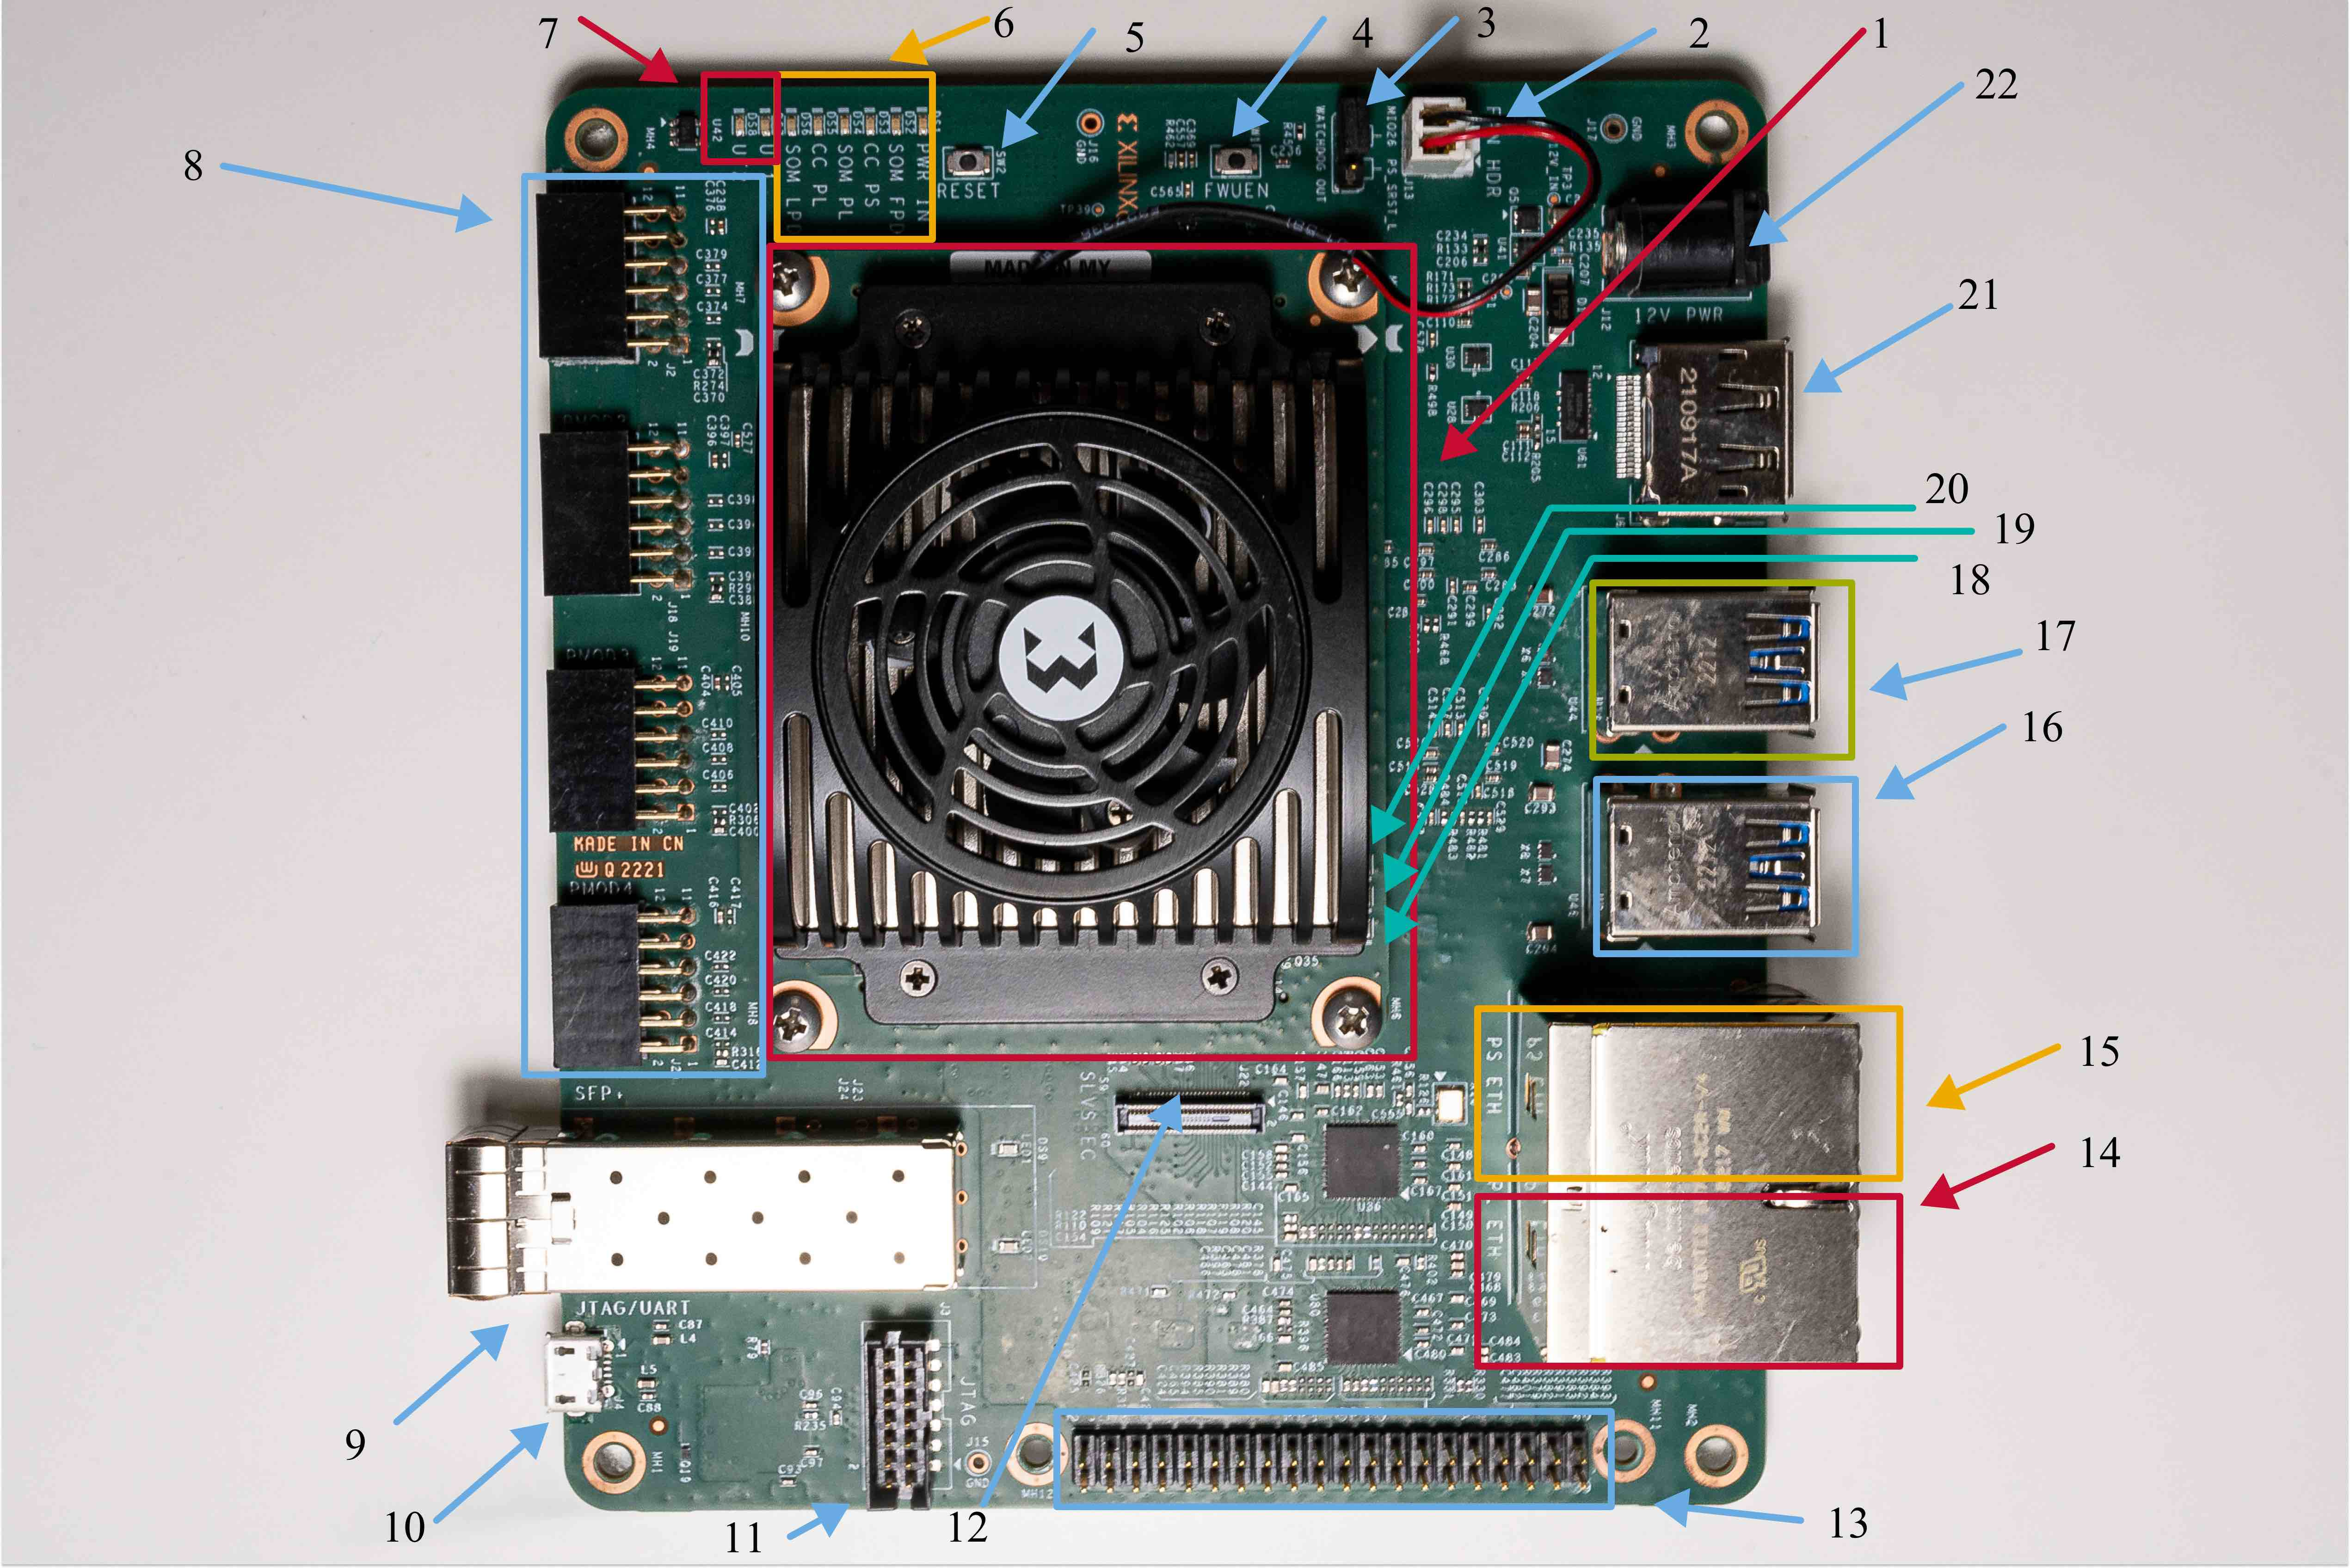
\includegraphics[width=1\textwidth]{src/jpg/xilinx-kria-foto-2-oznacene.jpeg} 
						\caption{Vývojová deska Xilinx Kria KR260 vrchní pohled s~vyznačením komponent.}
						\label{fig:xilinx-kria-foto-2-oznacene}
				\end{figure}


				\begin{figure}[H]
					\centering
						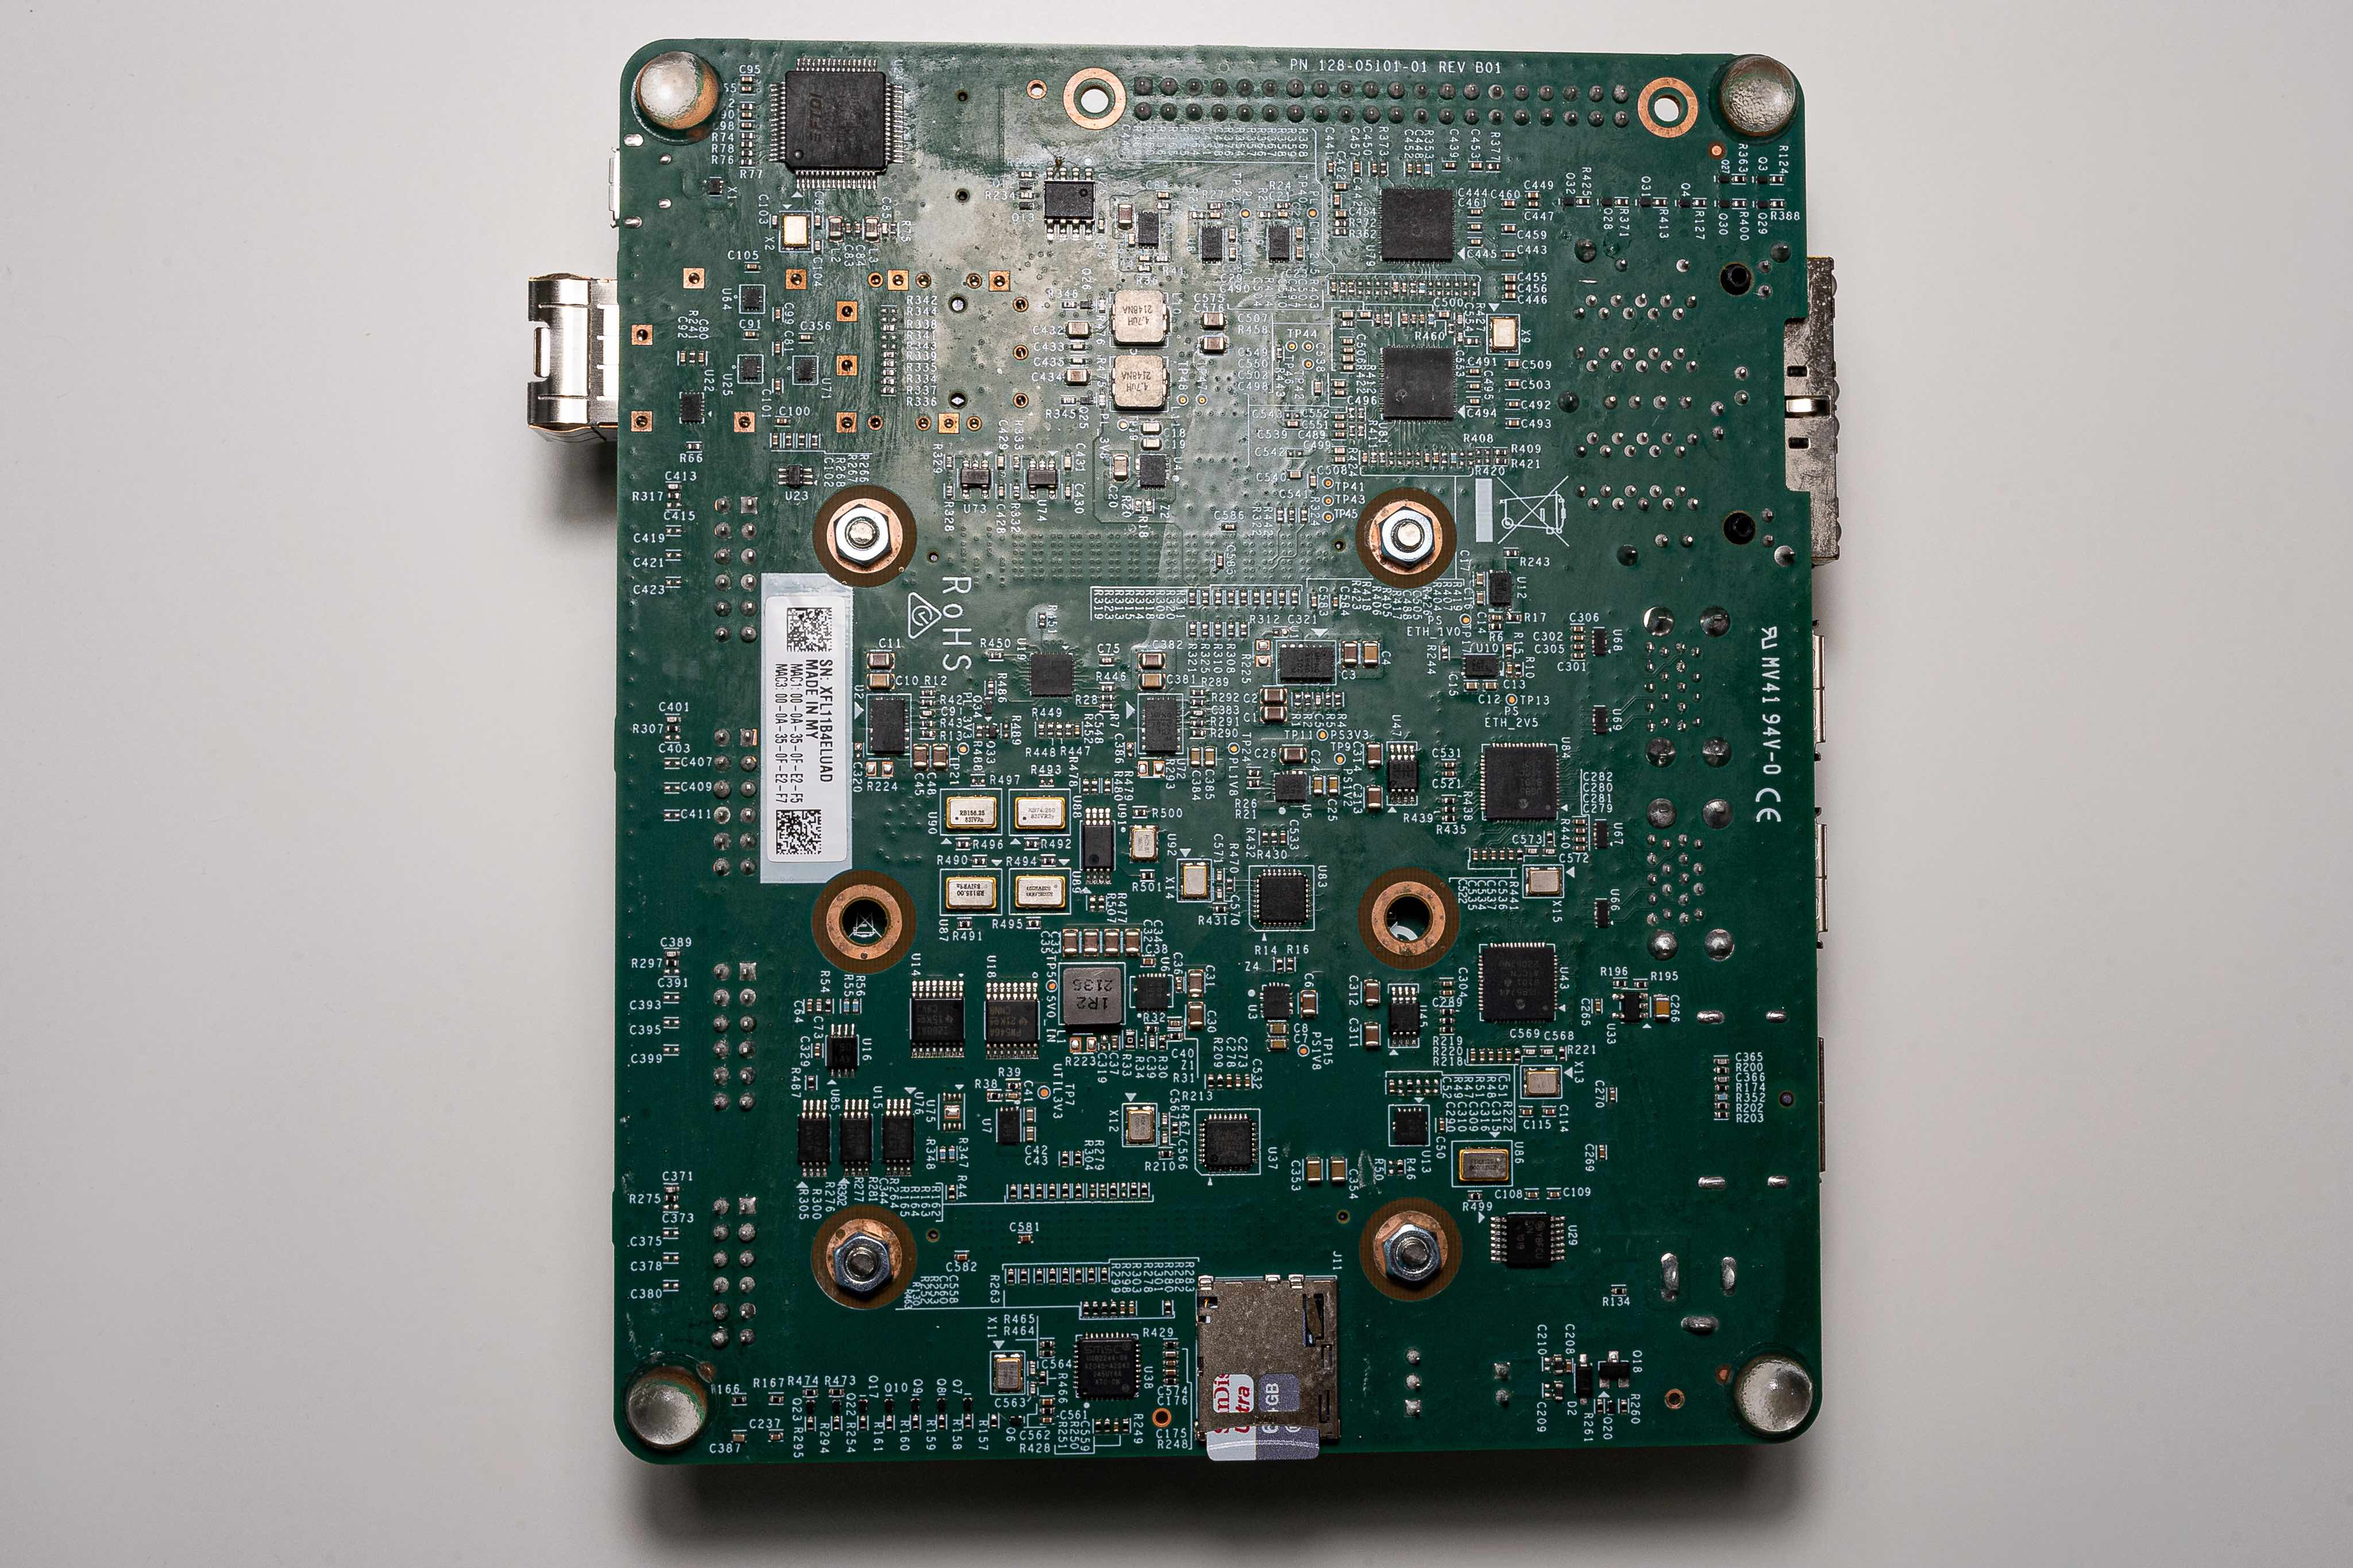
\includegraphics[width=1\textwidth]{src/jpg/xilinx-kria-foto-3.jpeg} 
						\caption{Vývojová deska Xilinx Kria KR260 – spodní pohled.}
						\label{fig:xilinx-kria-foto-3}
				\end{figure}
			
			
				\subsubsection{Dostupné K26 SOM}
					Moduly Kria K26 \gls{abbreviation:som} jsou dostupné v~několika variantách. V~roce 2022 jsou dostupné varianty \textit{Commercial} a \textit{Industrial}. Další dělení dvou hlavních variant je\gls{abbreviation:som} s~povoleným nebo zakázaným šifrováním. Varianty se odlišují označením Encryption Disabled (ED) a Encryption Enabled (-). Pokud je šifrování povoleno, je možné šifrovat konfigurační soubory a nebo ve vytvářených aplikacích využívat implementované \textit{crypto-accelerator} bloky. Encryption Enabled varianty jsou v~některých zemích zakázané a proto je důležité při výběru zboží dbát pokynů prodejce.
					\par Významné rozdíly \textit{Commercial} a \textit{Industrial} variant jsou uvedeny v~tab. \ref{tab:xilinx-kria-som-variants}.

					\begin{table}[htbp!]
						\centering
						\caption{Porovnání hlavních parametrů Kria K26 \gls{abbreviation:som} Commercial a Industrial. (informace a značení převzaty z~\cite{kria-k26-som-product-brief})}
						  \vspace*{0.15cm}
						   \resizebox{\textwidth}{!}
							{
								\begin{tabular}{!{\vrule width 2pt} l | c | c !{\vrule width 2pt}}\noalign{\hrule height 2pt}
								\rowcolor{codeblue}
								parametr & K26 Commercial \gls{abbreviation:som} & K26 Industrial \gls{abbreviation:som} \\
								\noalign{\hrule height 2pt}
								pracovní teplota & 0–85 °C & -40–100 °C\\ \hline
								záruka & 2 roky & 3 roky\\ \hline
								předpokládaná doba životnosti produktu & 5 let & 10 let\\ \hline 
								dostupnost produktu & 10 let & 10 let \\\noalign{\hrule height 2pt}
								\end{tabular}
							}
						\label{tab:xilinx-kria-som-variants}
					\end{table}

					Vývojová deska Xilinx Kria KR260 obsahuje dle informací výrobce \gls{abbreviation:som}, jež není určen pro nasazení do produkčních aplikací (non-production) a je v~teplotní třídě \textit{Commercial}. \cite{kria-k26-som-ds}
				

			\section{Porovnání představených SoC/SoM platforem pro řízení elektrických pohonů}
			V~předchozích kapitolách byly představeny dvě smysluplné (z~finančního i aplikačního hlediska), komerčně dostupné platformy, které je možné využít pro vývoj aplikací. Výběr byl zaměřen na \gls{abbreviation:soc} a \gls{abbreviation:som}, umístěných na vývojových deskách, které je možné využít pro vývoj požadované aplikace. Často po prvotním vývoji aplikace následuje uvědomění, jaké periferie by měla \gls{abbreviation:cc} obsahovat. Poté je možné pro velkoprodukci dané aplikace začít vyvíjet vlastní \gls{abbreviation:cc} a řešit integraci čipu/modulu na Printed Circuit Board (\gls{abbreviation:pcb}). V~této práci byly však využity již připravené vývojové desky, které je možné vzájemně porovnat v~několika ohledech.\par

			\subsection{Konektivita}
					Aby bylo možné komunikovat s~řízeným zařízením, tudíž vysílat řídící signály a získávat informace o~jeho stavu, je při hodnocení důležitým faktorem možnost připojení.\par
					Obě představené platformy disponují minimálně čtyřmi \gls{abbreviation:pmod} konektory s~12 piny (2x \gls{abbreviation:u-plus}, 2x \gls{abbreviation:gnd}, 8x \gls{abbreviation:io}), pomocí kterých je možné připojit senzory, převodníky nebo naopak ovládat drivery spínacích polovodičových součástek či výkonových polovodičových můstků. \gls{abbreviation:pmod} konektory využívá mnoho komerčně dostupných prvků jako jsou senzory, H můstky nebo \gls{abbreviation:adc}/\gls{abbreviation:dac} převodníky.\par
					Dalším důležitým faktorem konektivity je připojení pomocí Ethernetu. Xilinx Kria KR260 obsahuje 4 konektory, přičemž dva jsou připojeny přímo do \gls{abbreviation:ps} a dva do \gls{abbreviation:pl}. Digilent Zybo obsahuje pouze jeden Ethernet konektor.\par
					Pro připojení periferií nebo externích datových úložišť je možné využít konektor \gls{abbreviation:usb}. Protože Digilent Zybo Z7 je staršího data vydání, využívá pouze \gls{abbreviation:usb} 2.0, zatímco Xilinx Kria KR260 využívá připojení pomocí \gls{abbreviation:usb} 3.0.\par
					Pro připojení externího displeje je možné u~Zybo využít D-SUB (VGA) konektor. U~Kria KR260 novější Display Port.\par
					Digilent Zybo má na svém \gls{abbreviation:pcb} umístěny konektory pro výstup reproduktorů či vstup mikrofonu. Deska KR260 tyto konektory neobsahuje.\par
					Značným přínosem pro konektivitu Kria KR260 je Rraspberry Pi hardware attached on top (\gls{abbreviation:hats}) konektor, jež umožňuje připojení rozšiřovacích desek, určených pro Raspberry Pi.\par
					Pro \gls{abbreviation:ai} aplikace na KR260, které využívají externího obrazu, je možné připojit externí webkameru pomocí konektoru SLVS-EC.\par
					Posledním významným konektorem na \gls{abbreviation:cc} Xilinx Kria je \gls{abbreviation:sfp} konektor pro připojení optických vláken.

			\subsection{PS a PL}\label{subsec:ps-a-pl}
					Protože je porovnávaná deska Digilent Zybo a Xilinx Kria KR260 různého data vydání a také na jejich pořízení je třeba rozdílných finančních prostředků, odpovídají zdroje pro \gls{abbreviation:ps} a \gls{abbreviation:pl} daným cenám.\par
					Jak již bylo zmíněno v~sekci \hyperref[sec:vyvojova-deska-digilent-zybo]{\textit{Vývojová deska Digilent Zybo}}, \gls{abbreviation:ps} vývojové desky Digilent Zybo Zynq-7000 obsahuje dvoujádrový procesor Cortex-A9 s~taktovací frekvencí 650 MHz. Oproti tomu novější \gls{abbreviation:ps} desky s~Kria K26 \gls{abbreviation:som} obsahuje čtyřjádrový procesor Cortex®-A53 MPCore™ s~taktovací frekvencí až 1,5 GHz. \gls{abbreviation:som} je doplněn dvoujádrovým real-time procesorem Arm Cortex-R5F MPCore s~taktovací frekvencí až 600 MHz. \cite{digilent-zybo-reference-manual} \cite{kria-k26-som-ds}\par
					Dalším důležitým faktorem jsou zdroje pro \gls{abbreviation:pl}. Digilent Zybo disponuje pouze 17 600 \gls{abbreviation:luts}. Oproti tomu K26 \gls{abbreviation:som} obsahuje 117 120 \gls{abbreviation:luts}. Novější verze Digilent Zybo desek obsahuje novější verze Zynq čipu, který nabízí také 17 600 \gls{abbreviation:luts} (Zybo Z7-10) nebo 53 200 \gls{abbreviation:luts} (Zybo Z7-20). \cite{digilent-zybo-reference-manual} \cite{kria-k26-som-ds}\par
					Počet \gls{abbreviation:luts} v~této práci má značný vliv na možný rozsah vytvářené aplikace, která je počtem zdrojů (\gls{abbreviation:luts}, Flip-Flops, \gls{abbreviation:bram} atd.) velmi ovlivněna.\par
					Vlivem omezených zdrojů bylo možné i přes optimalizaci C++ kódu (pro dodržení load-compute-store modelu programování \cite{vitis-unified-software-platform-documentation-2022}) ukázkové akcelerované aplikace (kernelu) v~této práci umístit do \gls{abbreviation:pl} v~Digilent Zybo Z7 pouze $I$-$n$ model asynchronního motoru, jehož výsledkem byl transformační úhel \gls{symbol:theta-transform-angle} a složky vektoru magnetického toku rotoru \gls{symbol:psi2alpha-beta}. Oproti tomu při využití Kria~K26 \gls{abbreviation:som} je možné využít \gls{abbreviation:pl} pro výpočet $I$-$n$ modelu stroje, zjednodušeného modelu asynchronního motoru, regulátorů a invertoru.

			\subsection{Developer Experience}
					V~moderní době, kdy je kladen značný důraz na rychlost vývoje aplikace, je hodnotícím faktorem i developer experience (\gls{abbreviation:dx}). Tudíž jak je systém konfigurace a vytváření aplikací přívětivý pro vývojáře. U~Digilent Zybo Z7 byl používán postup vytvoření operačního systému \textit{PetaLinux} již s~pevně daným Device Tree (\gls{abbreviation:dt}), které bylo možné měnit pomocí rekonfigurace a následného opakování celého procesu tvorby systému a aplikace. To přinášelo značné časové prodlevy při ladění aplikace a vytvářeného \gls{abbreviation:pl} hardware.\par
					Při použití Xilinx Kria K26 \gls{abbreviation:som} je možné při tvorbě systému definovat kostru \gls{abbreviation:dt} pro \gls{abbreviation:ps}, kterou je poté možné do značného rozsahu upravovat pomocí Device Tree Overlay (\gls{abbreviation:dto}). Pomocí \gls{abbreviation:dto} je možné rekonfigurovat \gls{abbreviation:ip} vytvářené v~\gls{abbreviation:pl}. Změnou v~\gls{abbreviation:dto} je možné ovlivňovat funkčnost některých \gls{abbreviation:ip} v~\gls{abbreviation:pl} při chodu operačního systému \textit{PetaLinux}. Ovšem tyto úpravy mají určitá omezení a je vhodné Device Tree vhodně nakonfigurovat již při vytváření operačního systému \textit{PetaLinux}.\par
					Více informací o~chování a tvorbě \gls{abbreviation:dt}/\gls{abbreviation:dto}, zjištěných při realizaci této práce, je uvedeno v~části \hyperref[subsubsec:konfigurace-device-tree]{\textit{Konfigurace Device Tree}}.\par
					Digilent pro své výrobky vytvořil „board files“ a „constraints files“, které umožňují snazší konfiguraci \gls{abbreviation:ps} a \gls{abbreviation:pl} v~prostředí Vivado. Značným přínosem jsou „constraints files“, které umožňují snazší a rychlejší mapování fyzických pinů vývojové desky k~portům, pinům a rozhraní, vytvářených ve Vivado. Pro vývojovou desku Xilinx Kria KR260 jsou v~repozitáři ve Vivado již „board files“ obsaženy. Ovšem oficiální „constraints files“ nejsou od výrobce k~dispozici. Pro mapování pinů je nutné si vyžádat dokumentaci, pomocí které je možné odvodit požadované mapování a „constrains files“ vytvořit. Potřebná dokumentace pro odvození mapování je v~souborech \cite{kria-kr260-starter-kit-cc-schematics} a \cite{kria-k26-som-xdc}.
			
			\newpage
			\subsection{Aplikace a operační systém}\label{subsec:aplikace-a-operacni-system}
				Aplikace pro Digilent Zybo je možné vytvářet jako \textit{Bare Metal / Standalone} nebo jako aplikace pro operační systém \textit{PetaLinux}.\par
				Pro Xilinx Kria je možné využít \textit{Bare Metal / Standalone} přístup, \textit{PetaLinux} a také distribuci operačního systému Linux \textit{Ubuntu}. Výrobce na stránkách Wiki podpory produktů Xilinx zmiňuje, že poskytuje podporu převážně ve formě veřejného fóra na adrese \href{https://support.xilinx.com}{\textcolor{ctublue}{\textit{support.xilinx.com}}}. Oficiální podpora je vždy dostupná pro dvě poslední major verze softwarových nástrojů, které jsou součástí \textit{PetaLinux Tools} a~\textit{Xilinx~\gls{abbreviation:sdk}}. \cite{xilinx-wiki-atlassian-embedded-sw-support}\par
				Výrobce vytvořil pro Xilinx Kria ukázkové akcelerované aplikace, které je možné při využívání operačního systému \textit{Ubuntu} přímo stáhnout z~Kria App Store. V~plánu výrobce je vytvořit více aplikací, které by mohly sloužit jako výchozí bod pro vývojáře a byly by umístěny~v~Kria~App~Store. \cite{xilinx-appstore-for-kria-soms}\par
				\gls{abbreviation:ps} na porovnávaných vývojových deskách podporují PREEMPT\_\gls{abbreviation:rt} Linux Patch. K~tomuto patchi ovšem Xilinx, Inc. neposkytuje žádnou oficiální podporu a je nutné získávat informace přímo od autorů projektu na Wiki stránce \cite{wiki-linux-foundation-real-time-linux} nebo z~omezené podpory pomocí fóra. Více informací o~PREEMPT\_\gls{abbreviation:rt} Linux Patch \textit{PetaLinux} je v~sekci \hyperref[subsec:real-time-linux-patch]{\textit{RealTime Linux Patch}}.

\section{Zpětnovazební vektorová regulace}
	V~této práci bude využití platformy demonstrováno pomocí realizace simulace zpětnovazebního vektorového řízení asynchronního motoru. Zadání úlohy bylo převzato z~předmětu B1M14EPT. \cite{lipcak-bauer-ept-moodle}\par
	Hlavním záměrem této práce není představovat princip vektorové regulace, ale je vhodné pomocí blokového schématu nastínit její princip. Na obr. \ref{fig:foc-block} je zobrazeno obecné schéma zpětnovazební vektorové regulace. Naznačeným obecným způsobem by bylo možné realizovat fyzickou regulaci s~použitím vývojové desky a potřebných prvků (\gls{abbreviation:adc}, senzorů, \dots).\par
	Z~finančních důvodů je možné při spojení vinutí motoru do hvězdy a volby konstanty Clarkovi transformace \gls{symbol:konstanta-clarkovi-transformace-pri-wk-0} = $2/3$ měřit pouze dvě hodnoty napájecích proudů statoru motoru. Pro úplnost jsou naznačeny v~obr. \ref{fig:foc-block} všechny tři snímače. Pro měření otáčivé rychlosti motoru je možné použít inkrementální snímač a jeho výsledné impulzy zpracovávat pomocí \gls{abbreviation:ps} nebo \gls{abbreviation:pl}. Pokud by byl k~dispozici jiný druh snímače, je preferován prvek s~možností komunikace pomocí \gls{abbreviation:spi}, která splňuje požadavky na rychlé příjmání a odesílání hodnot.\par
	V~této práci byla realizována pouze simulace jednotlivých prvků \gls{abbreviation:foc}. Upravené blokové schéma simulace je zobrazeno na obr. \ref{foc-block-colored}.\par
	\textcolor{ctuyellow}{Žluté označení} symbolizuje, že se výpočty provádějí v~\texttt{krnl\_calculateCurVelModel}, tudíž v~prvním ze spouštěných kernelů v~podaplikaci \hyperref[subsec:cpu-fpga]{\textit{CPU/FPGA Model}}.\par
	\textcolor{ctugreen}{Zelené označení} symbolizuje provádění výpočtů výstupního napětí invertoru a modelu asynchronního motoru v~kernelu \texttt{krnl\_calculateInvMot}. \textcolor{ctublue}{Modře označený} blok symbolizuje, že je algoritmus prováděn v~\gls{abbreviation:ps}. \textcolor{ctublue}{Modře označená} proměnná je nastavována v~\gls{abbreviation:ps} a \textcolor{ctuyellow}{žlutě označená}, resp. \textcolor{ctugreen}{zeleně označená} je výstupem kernelu s~$I$-$n$ modelem, resp. s~modelem asynchronního motoru.\par
	Bloky (omezení a odvazbení) a měření napětí \gls{symbol:udc} nebyly v~aplikaci \hyperref[subsec:cpu-fpga]{\textit{CPU/FPGA Model}} implementovány. Bloky pro zpracování rychlosti otáčení byly vynechány z~důvodu, že mechanická otáčivá rychlost je přímo jeden z~výstupů modelu asynchronního motoru.

	\begin{figure}[htbp!]
		\centering
			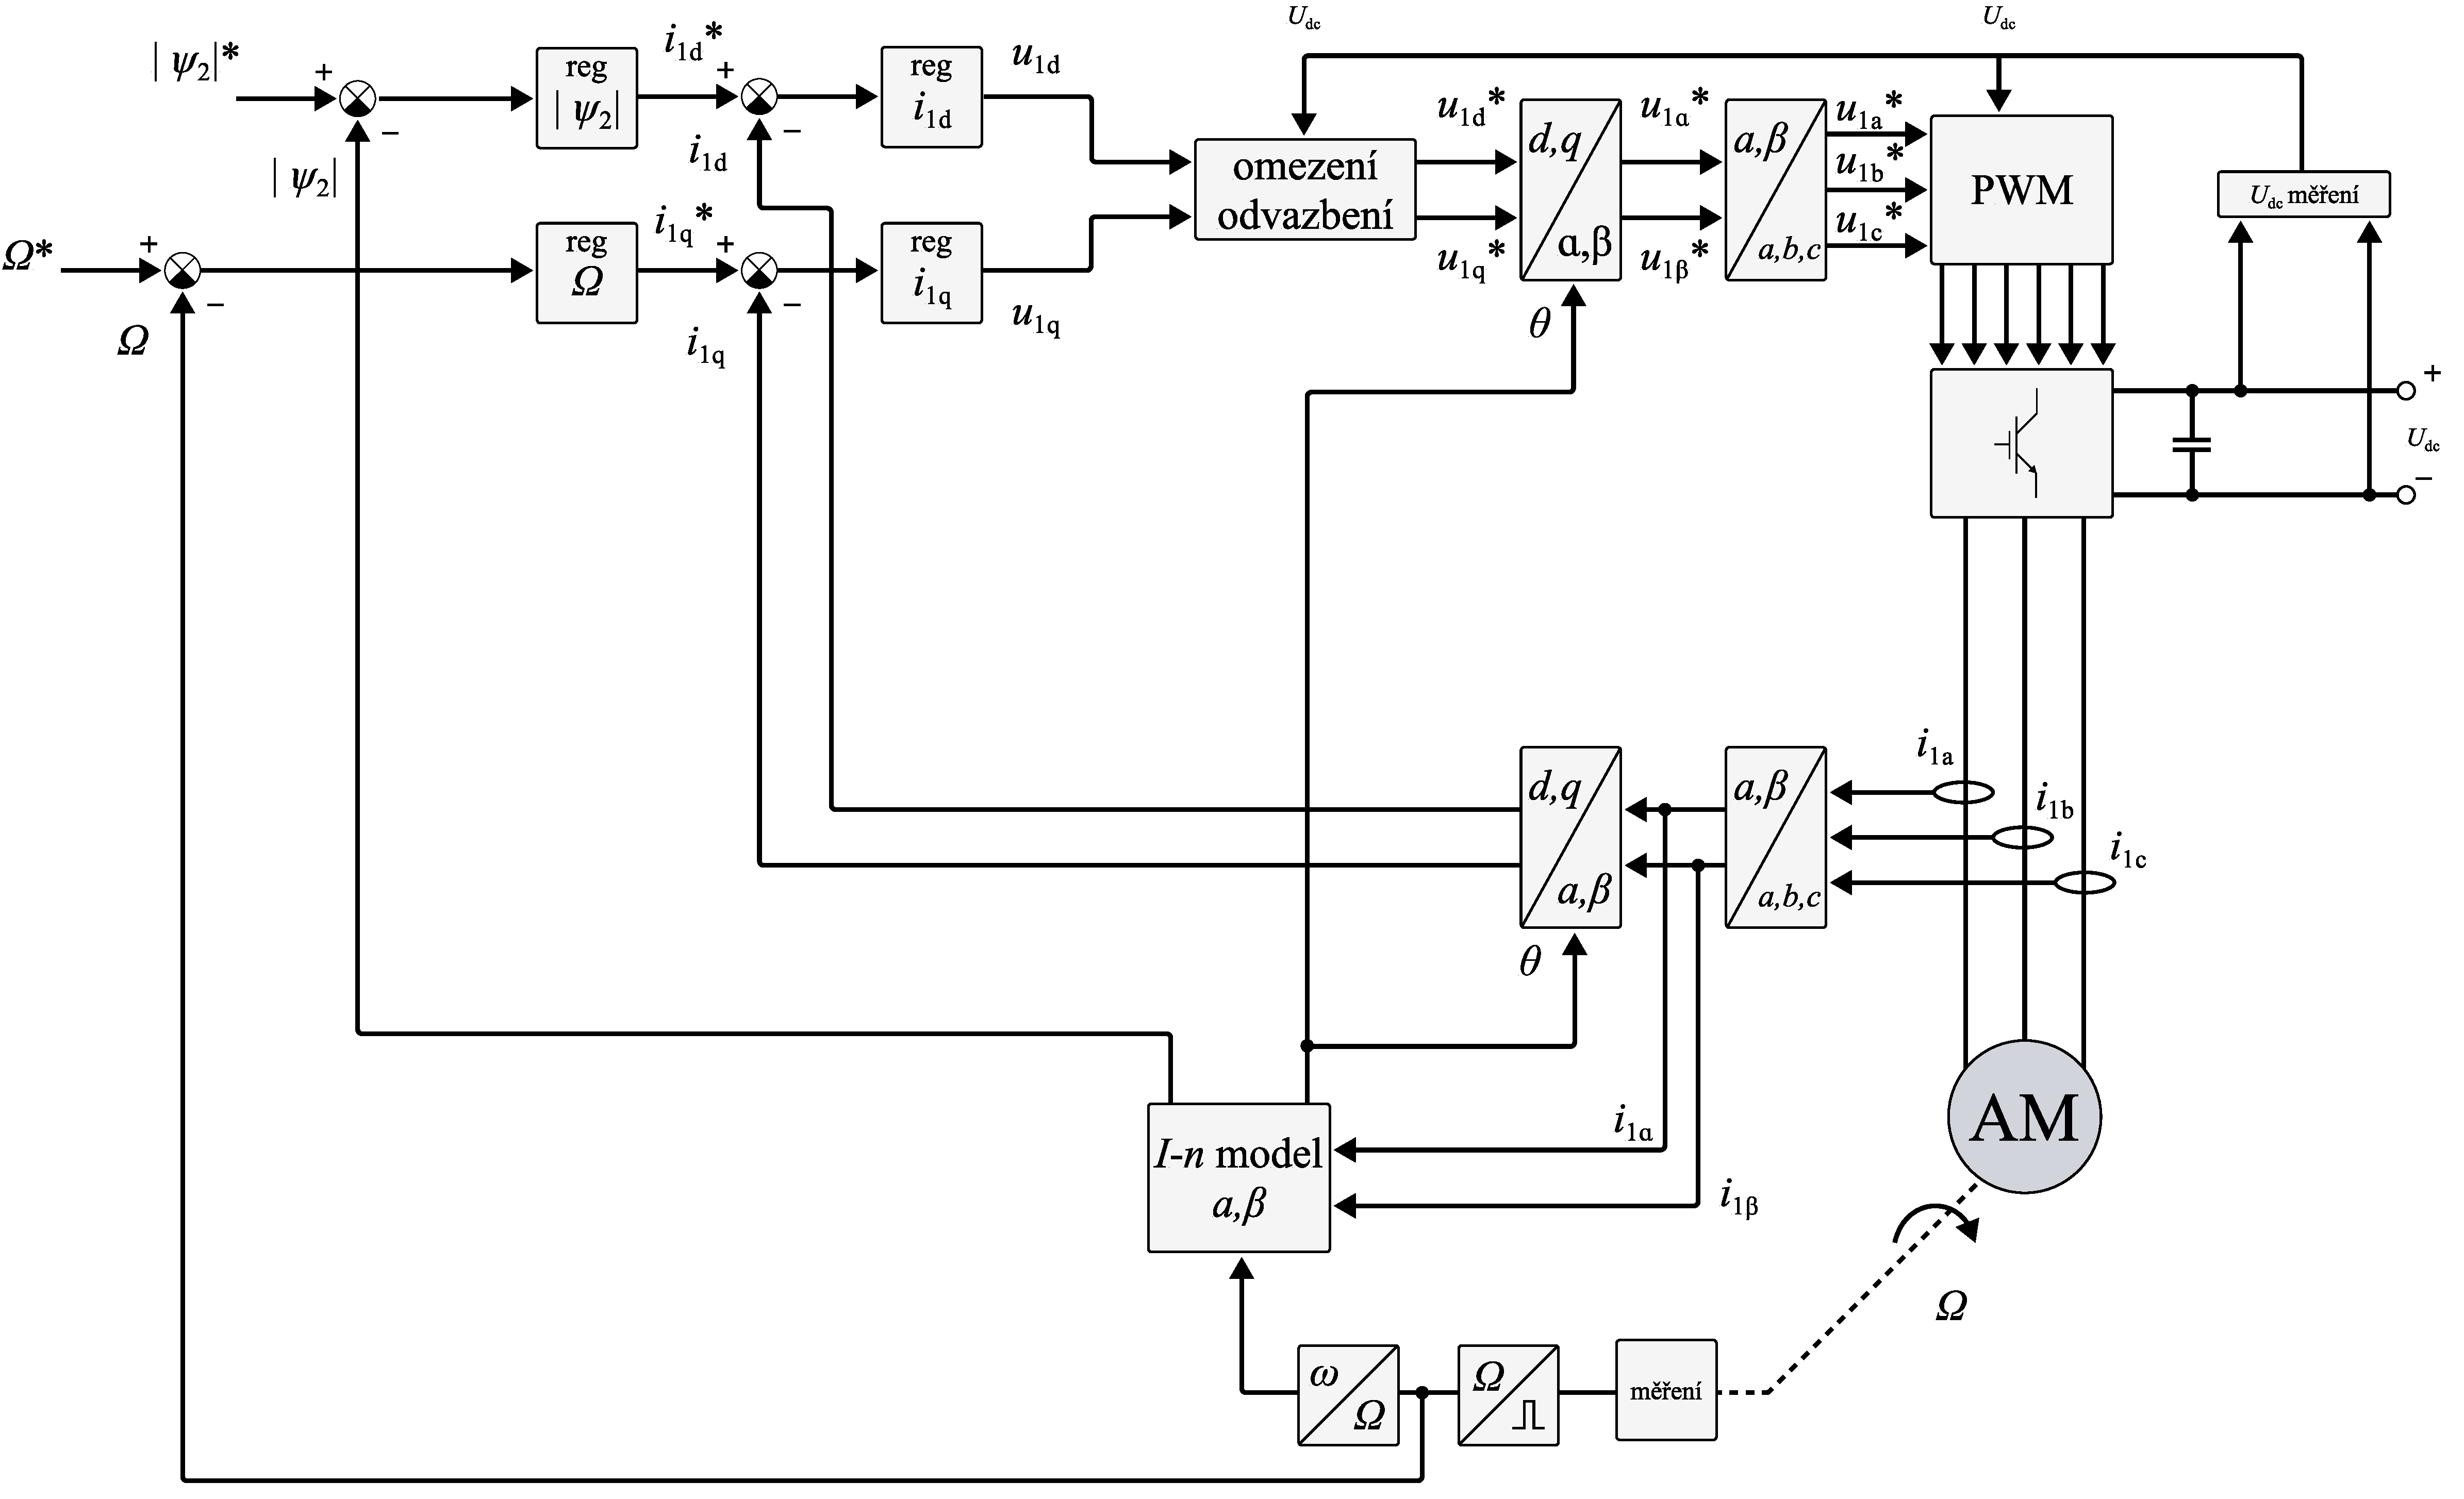
\includegraphics[width=1\textwidth]{src/pdf/foc-block.pdf} 
			\caption{Obecné schéma zpětnovazební vektorové regulace. (převzato z~\cite{lipcak-bauer-ept-moodle}, \cite{kobrle-elektricke-pohony}, upraveno)}
			\label{fig:foc-block}
	\end{figure}

	\begin{figure}[htbp!]
		\centering
			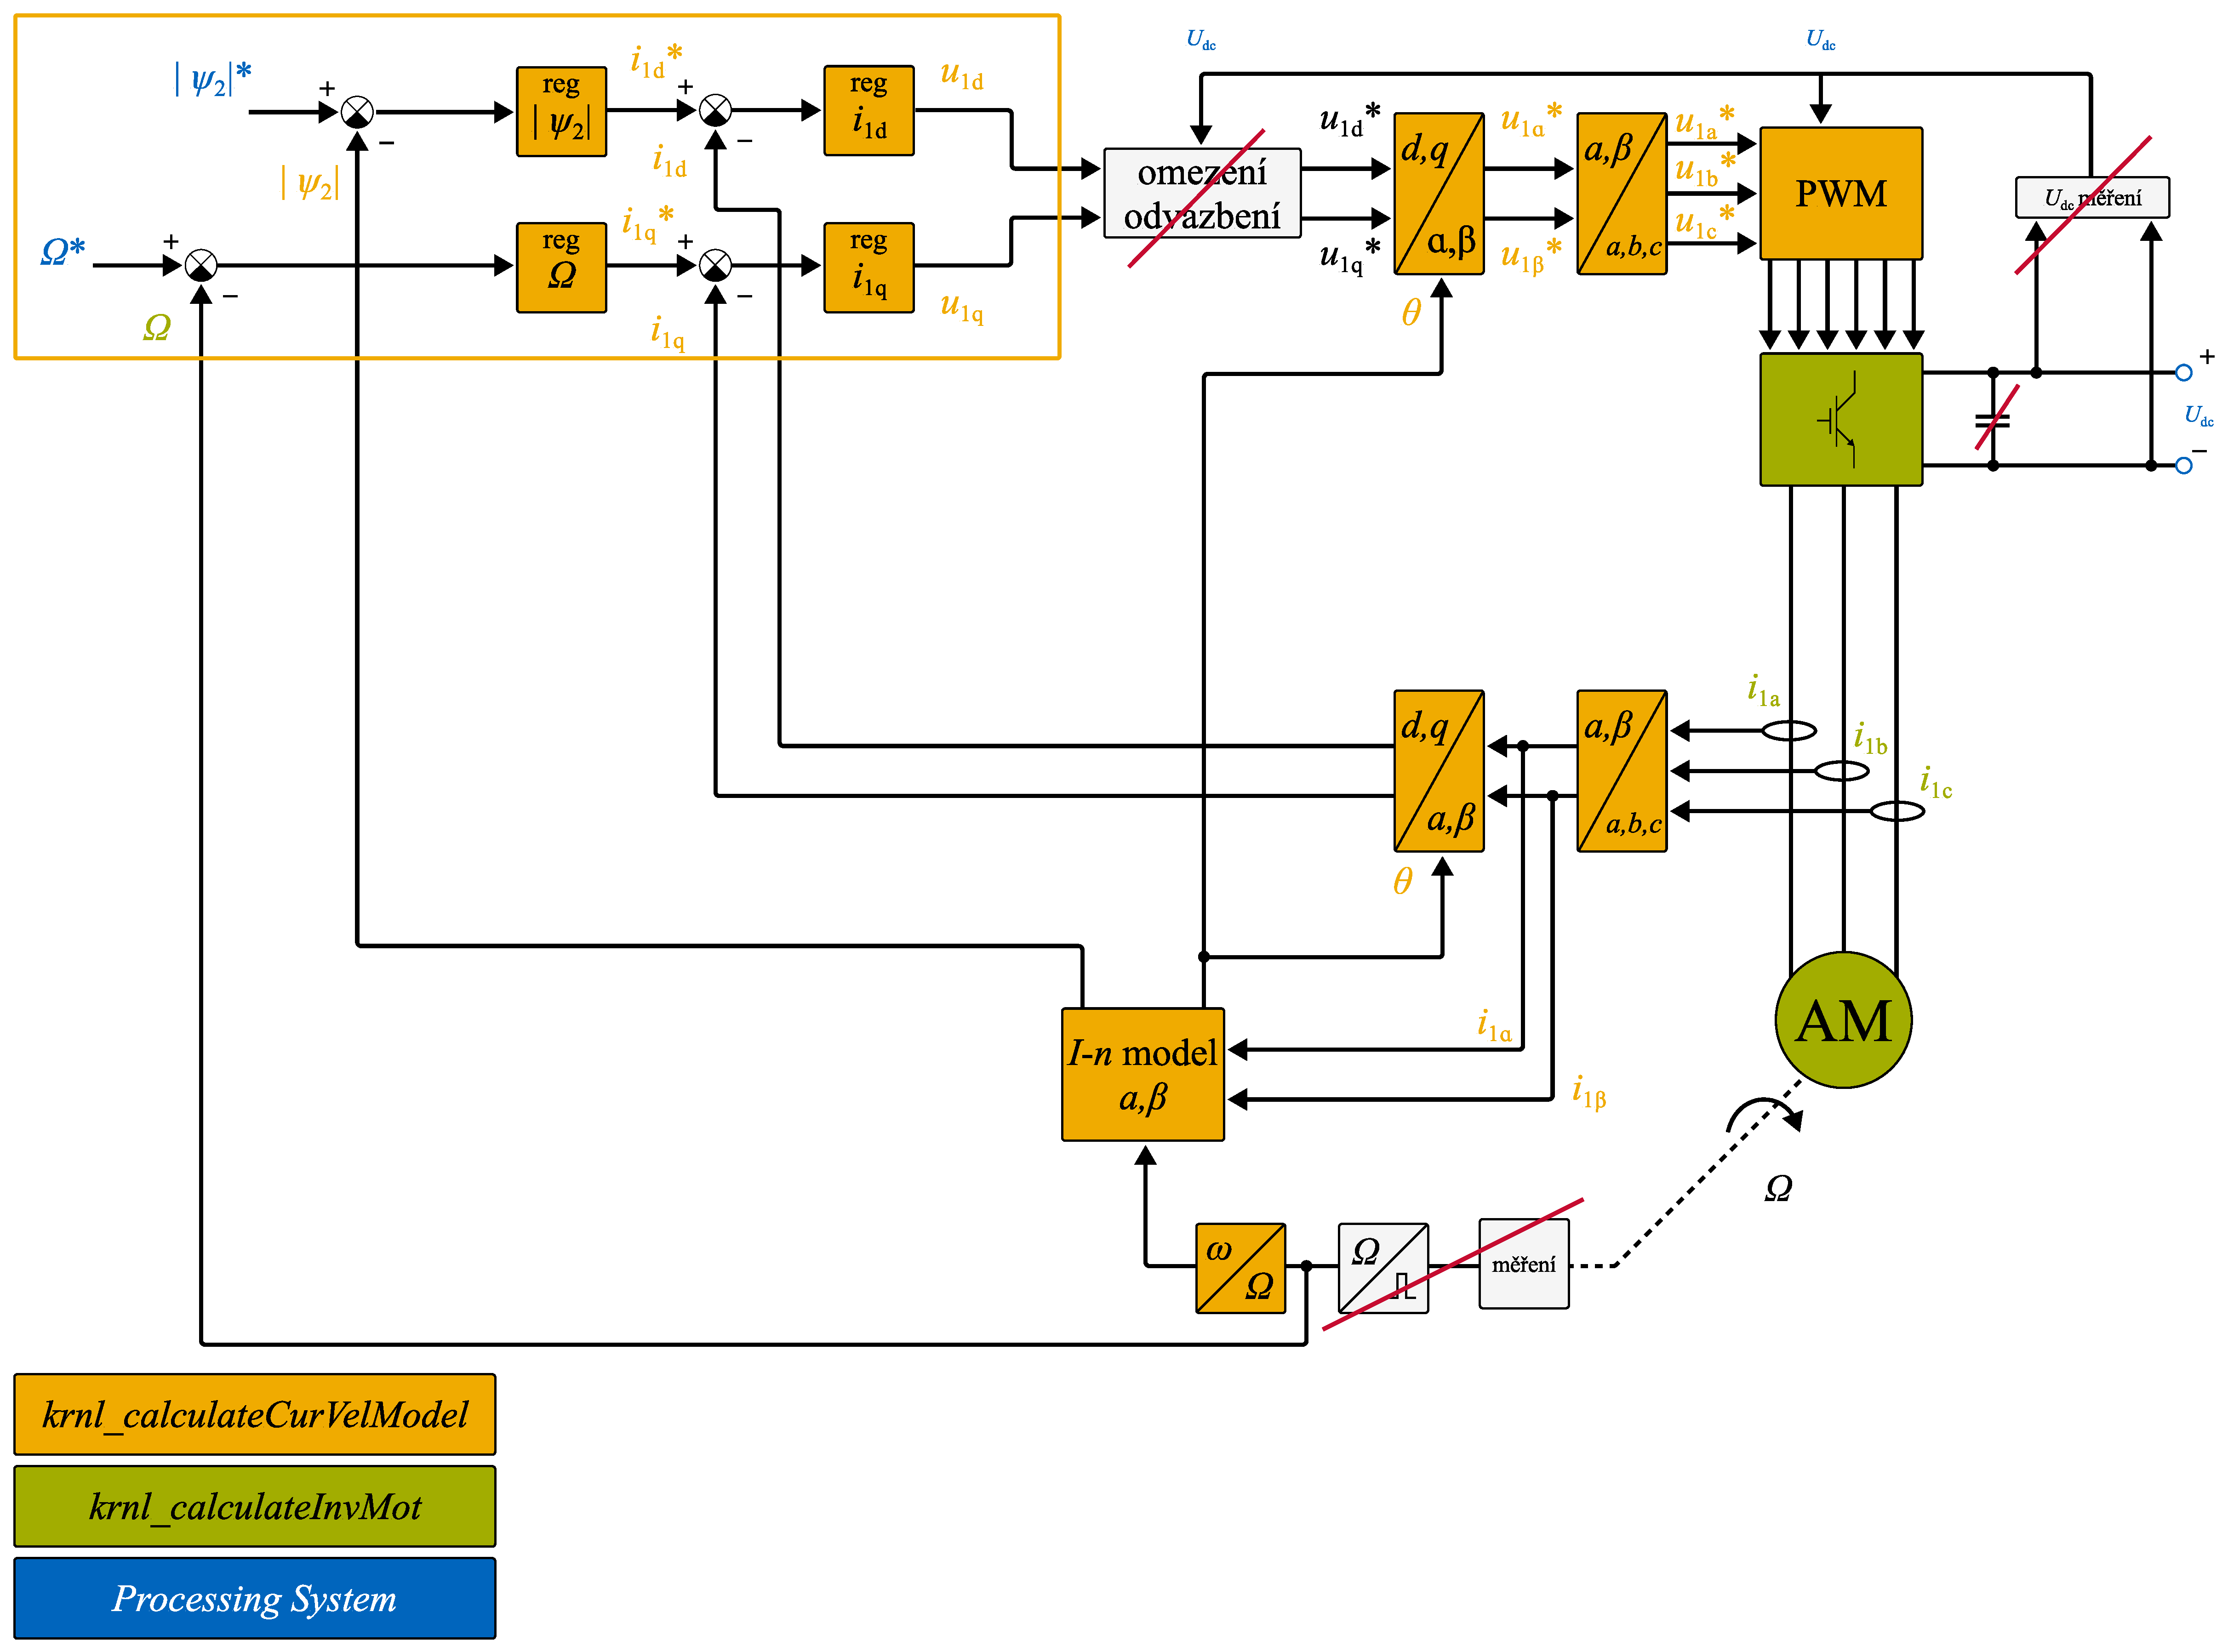
\includegraphics[width=1\textwidth]{src/pdf/foc-block-colored.pdf} 
			\caption{Simulační schéma zpětnovazební vektorové regulace, realizované v~této práci. (převzato z~\cite{lipcak-bauer-ept-moodle}, \cite{kobrle-elektricke-pohony}, upraveno)}
			\label{foc-block-colored}
	\end{figure}

\section{Model stroje}\label{sec:model-stroje}
	Jak již bylo představeno v~předchozích částech textu, akcelerované aplikace v~\gls{abbreviation:fpga} je možné použít na různé účely. Součástí této práce je realizace akcelerovaného výpočtu matematického modelu stroje. V~této práci bude k~demonstraci funkčnosti využit matematický model asynchronního motoru. Asynchronní motor bude modelován pomocí zjednodušeného modelu, zanedbávající některé jevy a pro \gls{abbreviation:foc} pomocí $I$-$n$ modelu.\par
	V~části \hyperref[subsec:ps-a-pl]{\textit{PS a PL}} je uvedeno, že vlivem omezených zdrojů je možné realizovat v~Digilent Zybo Z7 pouze $I$-$n$ model stroje. Ostatní výpočty je nutné realizovat v~\gls{abbreviation:ps}. V~Xilinx Kria K26 je díky většímu množství zdrojů možné realizovat větší část modelu v~\gls{abbreviation:pl} a pomocí \gls{abbreviation:ps} řešit pouze konfiguraci, řízení procesu akvizice dat nebo komunikaci.\par
	%% mám se v této celé kapitole více rozepsat o odvození modelu ASM
	%% schéma, princip činnosti, napěťové a tokové rovnice
	%% v optimalizace/úpravě modelu pro jazyk C++ mám se rozepsat o numerických metodách? RK4 bych použil
	%% kde prosím naleznu odvození těch rovnic na model stator proud rotor tok
	% clarkovy transformace - popsat
	% goniometrické funkce jsou v pure c++ v knihovně cmath, ve vitis jsou v hls_math.h
	% https://docs.xilinx.com/r/en-US/ug1399-vitis-hls/Vitis-HLS-Math-Library
	\subsection{Matematický popis „kompletního“ modelu stroje}\label{subsec:matematicky-popis-kompletniho-modelu-stroje}
	Parametry motoru, využívaného v~simulaci, byly získány z~výukových materiálů předmětu B1M14EPT \cite{lipcak-bauer-ept-moodle} a jsou uevedeny v~tab. \ref{tab:motor-stitkove-udaje} a v~tab. \ref{tab:motor-zmerene-parametry-stroje}.\par
	Motor je umístěn v~laboratoři č. H-26 na Fakultě elektrotechnické Českého vysokého učení technického v~Praze.
	\begin{minipage}[t]{0.47\textwidth}
        \vspace{\baselineskip}
        \begin{table}[H]
            \caption{Štítkové údaje stroje.}
            \centering
                \begin{tabular}{!{\vrule width 2pt} c | c !{\vrule width 2pt}}\noalign{\hrule height 2pt}
                    \gls{symbol:Pn} & 12 kW \\ \hline
                    \gls{symbol:Un} & 380 V~\\ \hline
                    \gls{symbol:Un} & 22 A\\ \hline
                    \gls{symbol:nn} & 1460 min$^{-1}$ \\ \hline
                    \gls{symbol:fn} & 50 Hz \\ \hline
                    \gls{symbol:cosphin} &  0.8 \\ \hline
                    \gls{symbol:pocet-polparu} & 2 \\ \noalign{\hrule height 2pt}
                \end{tabular}     
            \label{tab:motor-stitkove-udaje}
        \end{table}
        \end{minipage}% --- important, otherwise it wont be so nice
        \hfill
        \begin{minipage}[t]{0.47\textwidth}
            \vspace{0pt}
            \begin{table}[H]
                \caption{Změřené parametry stroje.}
                \centering
                    \begin{tabular}{!{\vrule width 2pt} c | c !{\vrule width 2pt}}\noalign{\hrule height 2pt}
                        \gls{symbol:r1} & 370 m$\Omega$ \\ \hline
                        \gls{symbol:r2} & 225 m$\Omega$ \\ \hline
                        \gls{symbol:l1sigma} & 2,27 mH \\ \hline
                        \gls{symbol:l2sigma} & 2,27 mH \\ \hline
                        \gls{symbol:lm} & 82,5 mH \\ \hline
                        \gls{symbol:l1} & 84,77 mH \\ \hline
                        \gls{symbol:l2} & 84,77 mH \\ \hline
						\gls{symbol:moment-setrvacnosti} & 0,4 kg$\cdot$m$^{2}$ \\ \noalign{\hrule height 2pt}
                    \end{tabular}     
                \label{tab:motor-zmerene-parametry-stroje}
            \end{table}
        \end{minipage}

        \vspace*{1cm}
\noindent Kde \gls{symbol:Pn}~(W) je jmenovitý výkon stroje, \gls{symbol:In} (A) je jmenovitý fázový proud stroje (efektivní hodnota), \gls{symbol:Un}~(V) je jmenovité sdružené napájací napětí stroje (efektivní hodnota), \gls{symbol:fn}~(Hz) je jmenovitá napájecí frekvence stroje, \gls{symbol:cosphin}~(-) je jmenovitý účinník stroje, \gls{symbol:nn}~(min$^{-1}$) jsou jmenovité otáčky stroje, \gls{symbol:pocet-polparu}~(-) je počet polpárů stroje, \gls{symbol:r1}~($\Omega$), resp. \gls{symbol:r2}~($\Omega$) je rezistivita statorového, resp. rotorového vinutí, \gls{symbol:l1sigma}~(H), resp. \gls{symbol:l2sigma}~(H) je statorová, resp. rotorová rozptylová  indukčnost stroje, \gls{symbol:lm} (H) je magnetizační indukčnost stroje, \gls{symbol:l1}~(H), resp.\gls{symbol:l2}~(H) je statorová, resp. rotorová indukčnost, \gls{symbol:moment-setrvacnosti} (kg$\cdot$m$^{2}$) je moment setrvačnosti hřídele.\par
Použitý model je založen na výpočtu složek vektorů statorového proudu \gls{symbol:prostorovy-vektor-statoroveho-proudu} a rotorového toku \gls{symbol:prostorovy-vektor-rotoroveho-toku} v~souřadnicovém systému $\alpha\beta$ spojeném se statorem. Tudíž při použití \gls{symbol:otaciva-rychlost-souradnicoveho-systemu}~$= 0$. Bude volena konstanta \gls{symbol:konstanta-clarkovi-transformace-pri-wk-0}~$= 2/3$. Poté bude stavový popis systému vypadat následovně. \cite{lipcak-bauer-ept-moodle}

\begin{equation}
    \frac{\dd{}}{\dd{t}}
    \begin{bmatrix}
        i_{1\alpha}\\
        i_{1\beta}\\
        \psi_{2\alpha}\\
        \psi_{2\beta}
    \end{bmatrix}
    =
    \begin{bmatrix}
        -\frac{R_2 L_\text{m}^{2} + L_2^2 R_1}{\sigma L_1 L_2^2} & 0 & \frac{L_\text{m} R_2}{\sigma L_1 L_2^2} & \frac{L_\text{m}}{\sigma L_1 L_2} \omega\\
        0 & - \frac{R_2 L_\text{m}^2 + L_2^2 R_1}{\sigma L_1 L_2^2} & - \frac{L_\text{m}}{\sigma L_1 L_2} \omega & \frac{L_\text{m} R_2}{\sigma L_1 L_2^2}\\
        \frac{L_\text{m} R_2}{L_2} & 0 & - \frac{R_2}{L_2} & -\omega\\
        0 & \frac{L_\text{m} R_2}{L_2} & \omega & -\frac{R_2}{L_2}
    \end{bmatrix}
    \begin{bmatrix}
        i_{1\alpha}\\
        i_{1\beta}\\
        \psi_{2\alpha}\\
        \psi_{2\beta}
    \end{bmatrix}
    +
    \begin{bmatrix}
        \frac{1}{\sigma L_1} & 0\\
        0 & \frac{1}{\sigma L_1}\\
        0 & 0\\
        0 & 0
    \end{bmatrix}
    \begin{bmatrix}
        u_{1\alpha}\\
        u_{1\beta}
    \end{bmatrix}.
\end{equation}
Stavový popis je vhodné doplnit o~další rovnice, jež budou v~simulaci využity.

\begin{equation}
    M = \frac{3}{2} p_\text{p} \frac{L_\text{m}}{L_2} (\psi_{2\alpha} i_{1\beta} - \psi_{2\beta} i_{1\alpha}),
\end{equation}

\begin{equation}
    M - M_\text{z} = J \frac{\dd{\Omega}}{\dd{t}},
\end{equation}
\begin{equation}
    \omega = p_\text{p} \Omega,
\end{equation}
kde \gls{symbol:sigma-rozptyl}~$= 1 - L_\text{m}^{2}/(L_1 L_2)$ (-) je tzv. rozptyl, \gls{symbol:i1alpha} (A) a \gls{symbol:i1beta} (A) jsou složky vektoru statorového proudu \gls{symbol:i1alpha-beta} (A), \gls{symbol:psi2alpha} (Wb) a \gls{symbol:psi2beta} (Wb) jsou složky vektoru rotorového magnetického toku \gls{symbol:psi2alpha-beta} (Wb), \gls{symbol:u1alpha} (V) a \gls{symbol:u1beta} (V) jsou složky vektoru statorového napětí \gls{symbol:u1alpha-beta} (V), \gls{symbol:pocet-polparu} (-) je počet polpárů stroje, \gls{symbol:elektricka-uhlova-rychlost} (s$^{-1}$) je elektrická úhlová rychlost hřídele, \gls{symbol:mechanicka-uhlova-rychlost} (s$^{-1}$) je mechanická úhlová rychlost hřídele, \gls{symbol:vnitrni-elektromechanicky-moment} (Nm) je vnitřní elektromechanický moment stroje a \gls{symbol:zatezny-moment} (Nm) je moment zátěžný. \cite{lipcak-bauer-ept-moodle}

	\subsection{I-n model asynchronního motoru}
		Jak již bylo v~předcházejících částech zmíněno, pokud není k~dispozici dostatečný počet \gls{abbreviation:luts} pro výpočet kompletního matematického modelu, je možné využít \gls{abbreviation:pl} na výpočet proudově-otáčkového, resp.~$I$-$n$ modelu a regulační procesy realizovat v~\gls{abbreviation:ps}.\par
		Popis $I$-$n$ modelu vychází ze základních rovnic, popisující asynchronní motor, uvedených např. v~\cite{kobrle-elektricke-pohony} a \cite{lipcak-bauer-ept-moodle} (rovnice jsou upraveny a přeznačeny dle moderních konvencí ale význam zůstává zachován). V~teorii prostorových vektorů je možné tedy psát soustavu rovnic

		\begin{equation}
			\underline{u_{1}^{k}} = R_1 \underline{i_{1}^{k}} + \frac{\dd{\underline{\psi_1^{k}}}}{\dd{t}} + \text{j} \omega_k \underline{\psi_1^{k}},
		\end{equation}
		\begin{equation}
			\underline{u_{2}^{k}} = R_2 \underline{i_{2}^{k}} + \frac{\dd{\underline{\psi_2^{k}}}}{\dd{t}} + \text{j} (\omega_k - \omega) \underline{\psi_2^{k}},
		\end{equation}
	
		\begin{equation}
			\underline{\psi_1^{k}} = L_1 \underline{i_1^{k}} + L_\text{m} \underline{i_2^{k}},
		\end{equation}
	
		\begin{equation}
			\underline{\psi_2^{k}} = L_2 \underline{i_2^{k}} + L_\text{m} \underline{i_1^{k}},
		\end{equation}

		kde \gls{symbol:u1-vektor}~(V) je prostorový vektor statorového napětí, \gls{symbol:u2-vektor}~(V) je prostorový vektor rotorového napětí, \gls{symbol:i1-vektor}~(A) je prostorový vektor statorového proudu, \gls{symbol:i2-vektor}~(A) je prostorový vektor rotorového proudu, \gls{symbol:prostorovy-vektor-statoroveho-toku}~(Wb) je prostorový vektor magnetického toku statoru, \gls{symbol:prostorovy-vektor-rotoroveho-toku}~(Wb) je prostorový vektor magnetického toku rotoru, \gls{symbol:elektricka-uhlova-rychlost}~(s$^{-1}$) je elektrická úhlová rychlost otáčení rotoru, \gls{symbol:otaciva-rychlost-souradnicoveho-systemu}~(s$^{-1}$) je úhlová rychlost otáčení použitého souřadnicového systému, \gls{symbol:r1}~($\Omega$), resp. \gls{symbol:r2}~($\Omega$) je rezistivita statorového, resp.~rotorového vinutí, \gls{symbol:l1}~(H), resp. \gls{symbol:l2}~(H) je statorová, resp. rotorová indukčnost a \gls{symbol:lm}~(H) je hlavní magnetizační indukčnost.\par
		$I$-$n$ model vychází z~předpokladu, že otáčivá úhlová rychlost souřadnicového systému \gls{symbol:otaciva-rychlost-souradnicoveho-systemu}~=~0 a tudíž model je odvozován v~souřadnicovém systému spojeným se statorem (souřadnicový systém $\alpha \beta$). Po vzolení daného souřadnicového systému pro soustavu rovnic platí

		\begin{equation}
			\underline{u_{1}^{\alpha \beta}} = R_1 \underline{i_{1}^{\alpha \beta}} + \frac{\dd{\underline{\psi_1^{\alpha \beta}}}}{\dd{t}},
		\end{equation}
		\begin{equation}\label{eq:alphabeta-napeti-rotor-rovnice-i-n-model}
			\underline{u_{2}^{\alpha \beta}} = R_2 \underline{i_{2}^{\alpha \beta}} + \frac{\dd{\underline{\psi_2^{\alpha \beta}}}}{\dd{t}} - \text{j} \omega \underline{\psi_2^{\alpha \beta}},
		\end{equation}
	
		\begin{equation}
			\underline{\psi_1^{\alpha \beta}} = L_1 \underline{i_1^{\alpha \beta}} + L_\text{m} \underline{i_2^{\alpha \beta}},
		\end{equation}
	
		\begin{equation}\label{eq:alphabeta-tok-rotor-rovnice-i-n-model}
			\underline{\psi_2^{\alpha \beta}} = L_2 \underline{i_2^{\alpha \beta}} + L_\text{m} \underline{i_1^{\alpha \beta}}.
		\end{equation}

		V~případě řízení asynchronního motoru s~kotvou nakrátko orientovaného na rotorový tok je dále z~rovnice \ref{eq:alphabeta-tok-rotor-rovnice-i-n-model} vyjádřen prostorový vektor \gls{symbol:i2alpha-beta}, který je dále dosazen do upravené rovnice \ref{eq:alphabeta-napeti-rotor-rovnice-i-n-model}, u~které je přepokládáno, že \gls{symbol:u2alpha-beta} = 0.\par
		Výsledná diferenciální rovnice pro prostorový vektor rotorového magnetického toku je

		\begin{equation}
			\frac{\dd{\underline{\psi_{2}^{\alpha \beta}}}}{\dd{t}} = \frac{R_2}{L_2}L_\text{m} i_1^{\alpha \beta} + j \omega \underline{\psi_2^{\alpha \beta}} - \frac{R_2}{L_2} \underline{\psi_2^{\alpha \beta}}.
		\end{equation}

		Rozepsáním představené diferenciální rovnice do reálné a imaginární složky vznikne soustava diferenciálních rovnic $I$-$n$ modelu.

		\begin{equation}\label{eq:i-n-model-psi-2-diff-for-rk-4}
			\begin{gathered}
				\frac{\dd{\underline{\psi_{2\alpha}}}}{\dd{t}} = \frac{L_\text{m} R_2}{L_2} i_{1\alpha} - \frac{R_2}{L_2} \psi_{2\alpha} - \omega \psi_{2\beta},\\\frac{\dd{\underline{\psi_{2\beta}}}}{\dd{t}} = \frac{L_\text{m} R_2}{L_2} i_{1\beta} - \frac{R_2}{L_2} \psi_{2\beta} + \omega \psi_{2\alpha}.
			\end{gathered}
		\end{equation}


\section{Použité nástroje pro vývoj aplikace pro PS a PL}
V~této části jsou představeny jednotlivé nástroje, využívané při tvorbě programu pro \gls{abbreviation:ps} a akcelerované aplikace (kernelu) realizované na \gls{abbreviation:pl}. Je důležité zmínit, že v~\gls{abbreviation:ps} je skutečně spouštěn zkompilovaný program vytvářený pomocí jazyka C, C++ nebo Python. Na \gls{abbreviation:pl} je ovšem vytvořen \gls{abbreviation:hw}, který reprezentuje myšlené algoritmy aplikace. Tento \gls{abbreviation:hw} je popisován pomocí nízkoúrovňových jazyků, do kterých je algoritmus převeden pomocí~\gls{abbreviation:hls} z~jazyka C. Není tudíž korektně správné mluvit o~tom, že se vytváří program pro \gls{abbreviation:fpga}. Z~toho důvodu bude v~této práci používáno označení pro vytváření \gls{abbreviation:hw} na \gls{abbreviation:pl} \textit{vytváření kernelu} (creation of the kernel). Označení \textit{kernel} je myšleno v~odlišném významu než je využíváno v~části \hyperref[subsec:real-time-linux-patch]{\textit{RealTime Linux Patch}}.\par
	% Také jsou v~této části představeny postupy využívání vývojových nástrojů, které vedou k~úspěšné tvorbě aplikace.\par
Tvorba akcelerované aplikace může být obecně prováděna více způsoby. Tento způsob závisí na použitém vývojovém nástroji pro daný \gls{abbreviation:hw}. V~této práci je využíváno \gls{abbreviation:som} od firmy Xilinx, proto je výhodné využívat již připravené nástroje, které umožní snazší vývoj \gls{abbreviation:sw}, tvorbu \gls{abbreviation:hw} a přípravu systému na \gls{abbreviation:ps}.\par
	V~této práci veškerý používaný \gls{abbreviation:sw} od firmy Xilinx je po registraci volně dostupný ke stažení na \cite{xilinx-downloads}.
		\subsection{Xilinx Vivado}\label{subsec:xilinx-vivado}
			Xilinx Vivado je nástroj, používaný pro tvorbu \gls{abbreviation:hw} architektury, resp. platformy, pro kterou bude v~další části postupu možné vytvořit akcelerovanou aplikaci. Ve Vivado je možné tvořit \gls{abbreviation:hw} návrh, převeditelný do \gls{abbreviation:hdl}, který bude spustitelný v~\gls{abbreviation:pl} bez použití Vitis \gls{abbreviation:hls}. Pro vývojáře \gls{abbreviation:hw} na \gls{abbreviation:fpga} může sloužit i jako hlavní vývojářský nástroj.\par
			Se znalostí \gls{abbreviation:vhdl} je možné ve Vivado vytvářet požadovaný \gls{abbreviation:hw} design, ovšem tvorba designů ve Vivado s~využitím \gls{abbreviation:vhdl} je relativně náročnou záležitostí a není předmětem této práce. Využití \gls{abbreviation:vhdl} je však nevyhnutelnou součástí budoucího výzkumu využití těchto platforem pro řízení elektrických pohonů.\par
			Xilinx Vivado je součástí instalačního balíčku \textit{Xilinx Unified Installer}, dostupného z~\cite{xilinx-downloads}. Součástí balíčku verze 2022.2 \gls{abbreviation:sfd} je nástroj \hyperref[subsec:xilinx-vitis]{\textit{Xilinx Vitis}}. Je doporučeno instalovat oba tyto programy a vyvarovat se oddělené instalace, jež může přinášet problémy se vzájemnou i zpětnou kompatibilitou jednotlivých nástrojů.
		\subsection{Xilinx Vitis}\label{subsec:xilinx-vitis}
		Xilinx Vitis je nástroj, který slouží k~vytváření akcelerovaných aplikací na zařízení firmy Xilinx. Tento nástroj obsahuje základní vrstvu s~názvem Xilinx Vitis \gls{abbreviation:hls}, která slouží jako jádro převodu vytvářených aplikací v~C, C++ a OpenCL do \gls{abbreviation:rtl}. V~programu Xilinx Vitis bude vytvářena největší část aplikace, proto je vhodné nastínit postup, jakým Vitis pracuje.
		\par
		Nejprve je vytvořen tzv. „host program“ bežící na \gls{abbreviation:ps}, který je vyvíjen v~C/C++ jazyku (popř. Python), používající Xilinx Runtime (\gls{abbreviation:xrt}) Application Programming Interface (\gls{abbreviation:api}). Tento program je následně kompilován pomocí g++ kompilátoru, který vytvoří spustitelný soubor pro procesor. Tento host program komunikuje s~akcelerovanou částí aplikace (kernel), umístěné v~\gls{abbreviation:pl}. Blok \textit{ARM x86 host Application Compilation} na obr. \ref{fig:vitis-development-flow} naznačuje, jakým způsobem je vytvářena aplikace pro host procesor. \cite{vitis-unified-software-platform-documentation-2022}\par
		Poté Vitis \gls{abbreviation:hls} compiler přeloží C/C++ zdrojový kód pro kernel do register transfer level (\gls{abbreviation:rtl}) (úrovně registrů). Produkty této kompilace mají příponu „.xo“ (Xilinx Object) a mohou být spojovány do binárního souboru s~příponou „.xclbin“ pomocí Vitis linkeru. Souborem \textit{kernel.xclbin} je poté možné nakonfigurovat \gls{abbreviation:pl}. \cite{vitis-unified-software-platform-documentation-2022}\par
		Na obr. \ref{fig:vitis-development-flow} je blokově znázorněn postup tvorby spustitelné aplikace v~programu Vitis. Tento diagram předpokládá, že již byla vytvořena \gls{abbreviation:hw} platforma ve Vivado a \textit{PetaLinux} systém.\par
		Produkty větví tvorby programu pro \gls{abbreviation:ps} a konfigurace pro \gls{abbreviation:pl} je po jejich dokončení možné použít v~daném heterogenním systému. Host program zařídí nakonfigurování \gls{abbreviation:pl} pomocí souboru \textit{kernel.xclbin} a následné zpracování výsledků. Blok s~názvem \textit{Running the Application} je vykonáván v~prostředí \textit{PetaLinux} v~simulátoru (QEMU) nebo na fyzickém zařízení (vývojová deska).
		\begin{figure}[htbp!]
			\centering
			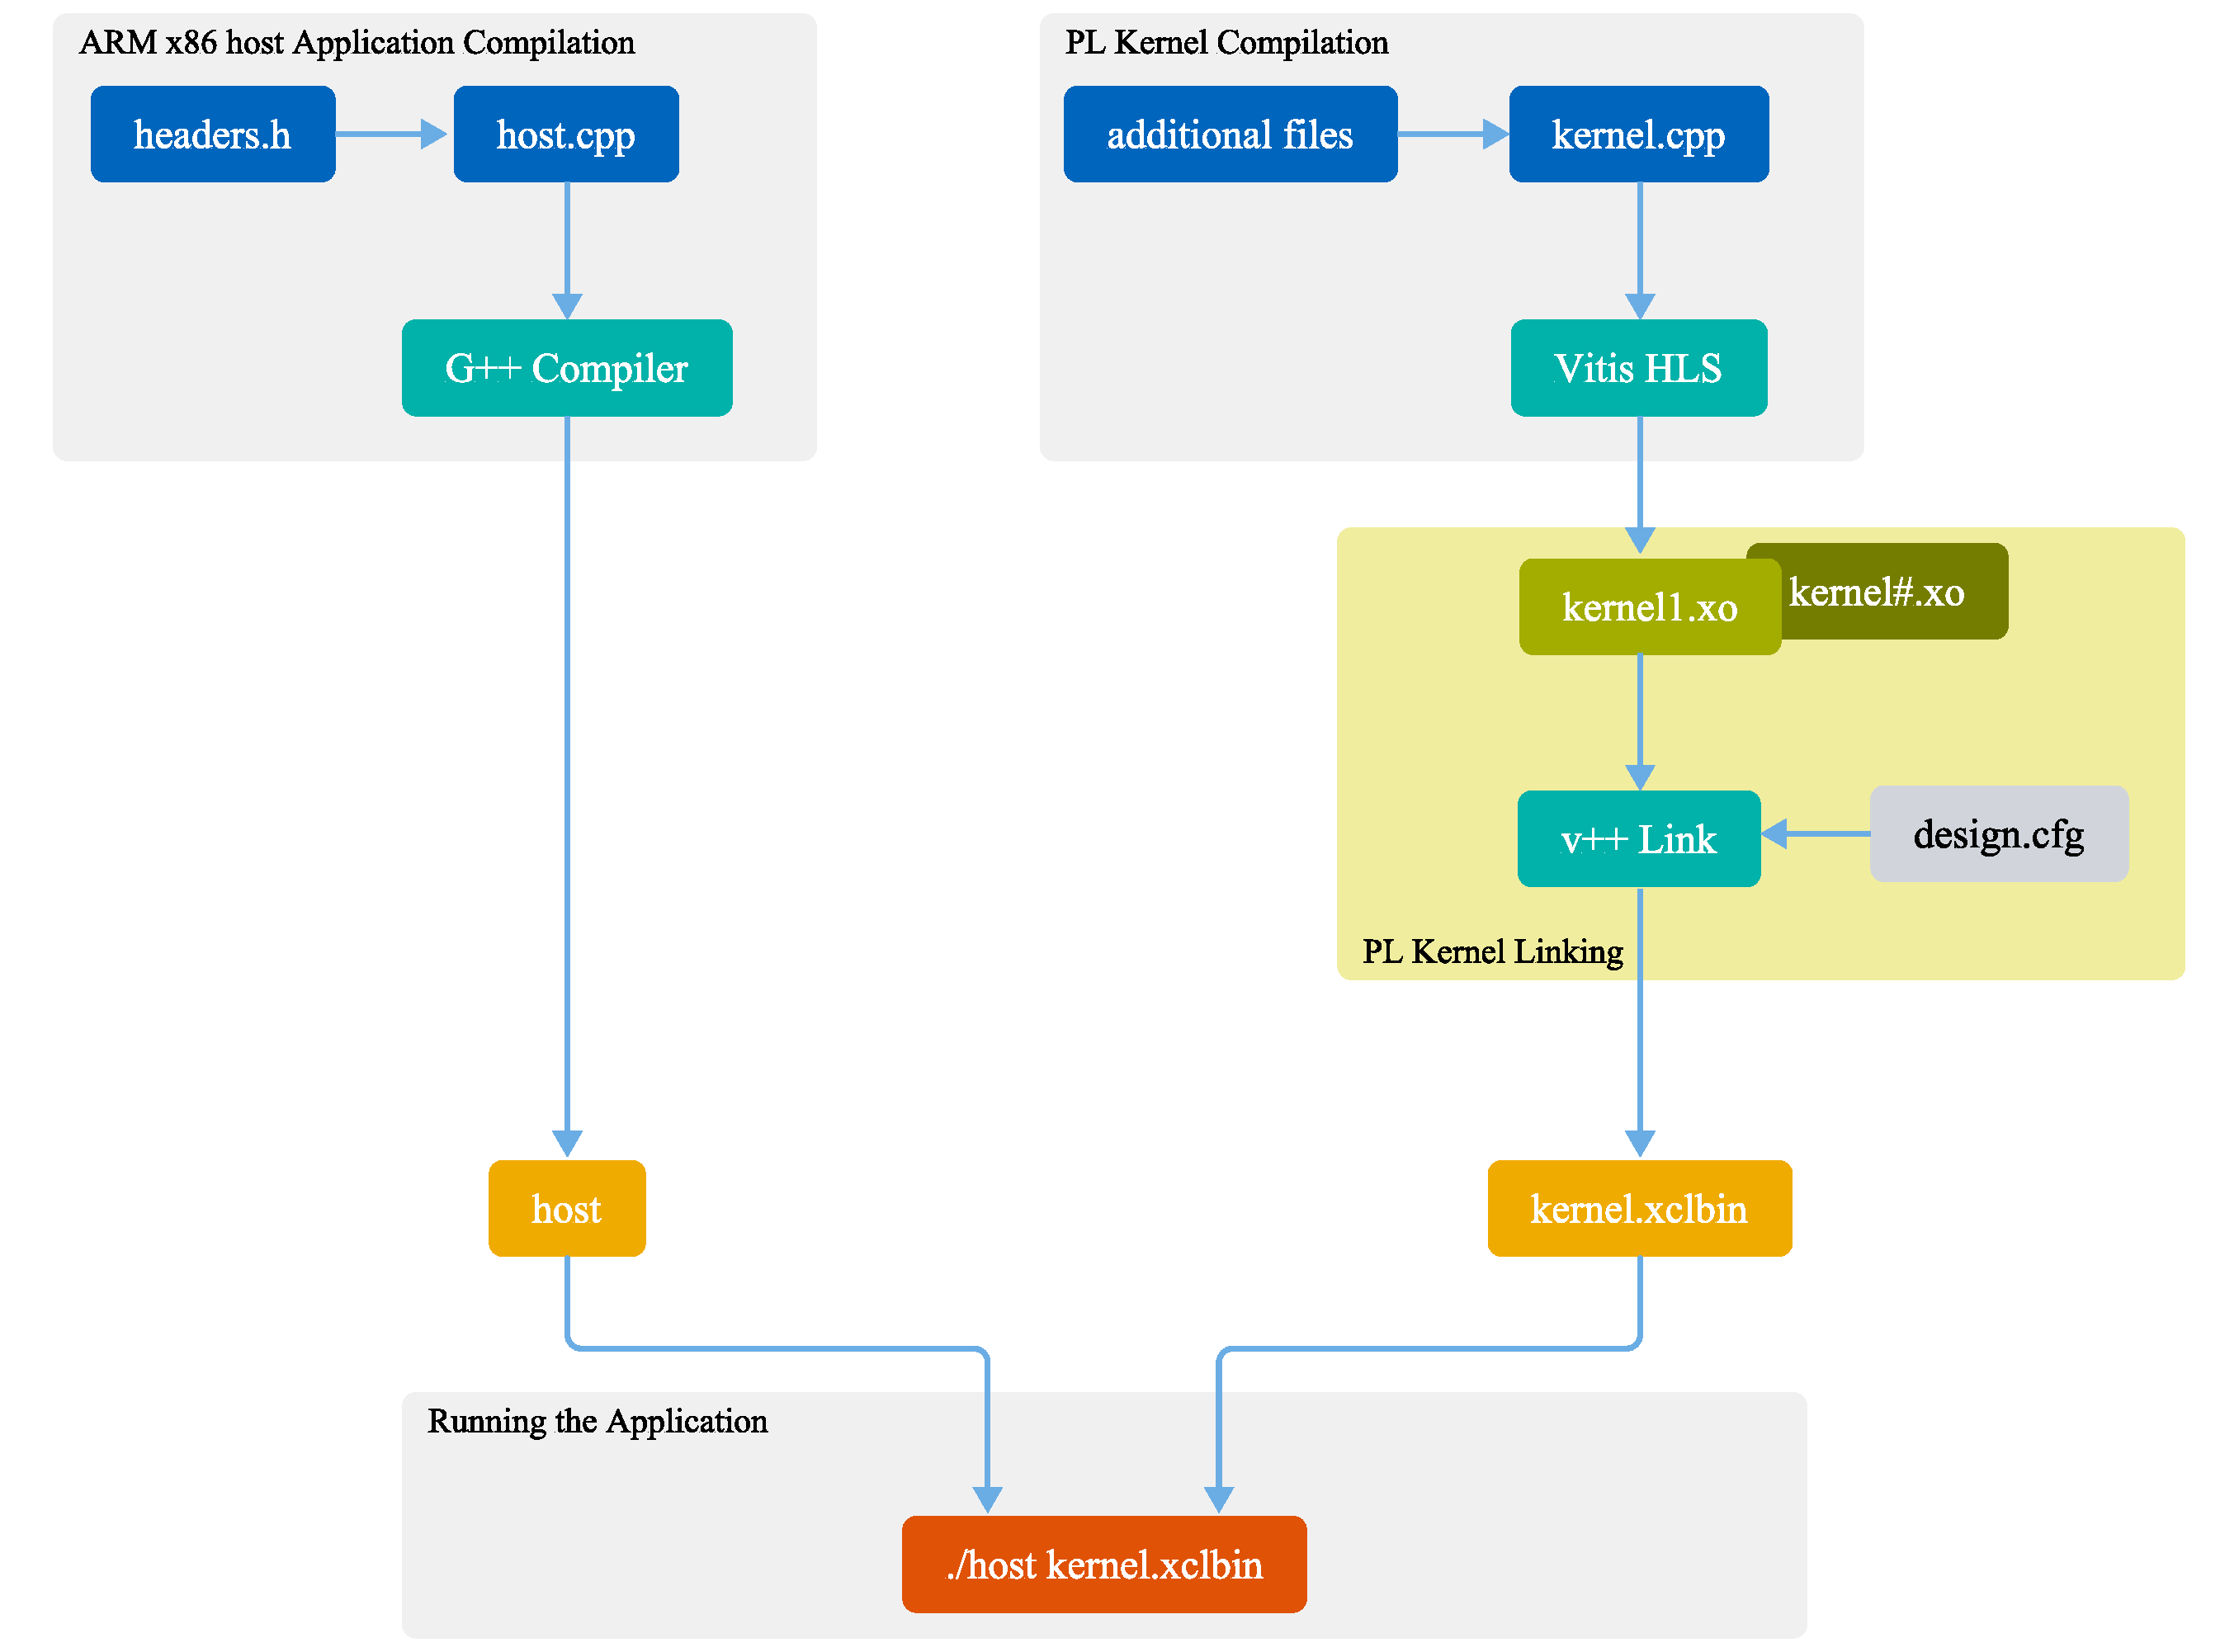
\includegraphics[width=1\textwidth]{src/pdf/vitis-development-flow.pdf}
			\caption{Blokový diagram tvorby spustitelné aplikace v~prostředí Vitis. (převzato z~\cite{vitis-unified-software-platform-documentation-2022}, upraveno)}
			\label{fig:vitis-development-flow}
		\end{figure}
		
		\subsection{PetaLinux Tools}\label{subsec:petalinux-tools}
			\textit{PetaLinux Tools} je nástroj, který slouží k~vytvoření systému \textit{PetaLinux}, jež bude spuštěn na \gls{abbreviation:ps} v~daném \gls{abbreviation:som} nebo \gls{abbreviation:soc}. Z~tohoto systému je poté možné spouštět navazující programy host (na \gls{abbreviation:ps}) a kernel (na \gls{abbreviation:pl}).\par
			\textit{PetaLinux} systém je možné nakonfigurovat dle požadavků aplikace. Při tvorbě tohoto systému je možné konfigurovat jádro systému (kernel), balíčky, které budou do systému nainstalovány, vytvořit uživatele systému nebo vybrat, kde v~paměti bude systém umístěn (\gls{abbreviation:ram}, \gls{abbreviation:sd} karta apod.). \cite{xilinx-petalinux}\par
			V~případě tvorby systému, který je konfigurovaný uživatelem, je třeba postupovat obezřetně a dodržovat nastavené postupy konfigurace, protože v~případě chyby je nutné překonfigurovat chybnou část nebo někdy kompletní systém. Tvorba \textit{PetaLinux} systému je časově náročný postup, u~něhož je problematický debugging.\par
			Pro funkční instalaci \textit{PetaLinux Tools} je nutné mít v~systému, kde bude docházet k~tvorbě \textit{PetaLinux} systému, nainstalované správné verze systémových a aplikačních balíků, které jsou nutnou prerekvizitou tvorby \textit{PetaLinux}. Požadavky na balíky je možné nalézt při nahlédnutí do dokumentace \cite{petalinux-tools-documentation-2022} instalované verze \textit{PetaLinux Tools}. V~dokumentaci v~sekci \textit{Installation Reguirements} se nachází odkaz\\označený \textit{PetaLinux <version> Release Notes}, který ve spodní části obsahuje stáhnutelný soubor\\\textit{<version>\_PetaLinux\_Package\_List.xlsx}, jež obsahuje seznam požadovaných balíků a jejich verze. Bez použití podporovaných balíků by nepracoval nástroj \textit{PetaLinux Tools} správně.

		\subsection{RealTime Linux Patch}\label{subsec:real-time-linux-patch}
			Protože operační systém Linux nebyl původně navrhován pro využití v~embedded systémech, ale v~obecných zařízeních jako jsou servery a stolní počítače, nebyl tento systém vhodný pro řešení úloh v~reálném čase (real time, \gls{abbreviation:rt}). Proto se objevila snaha upravit tento systém takovým způsobem, aby jej bylo možné v~\gls{abbreviation:rt} systémech využívat.\par
			Real time systémy je dle \cite{the-real-time-linux-kernel-survey-on-preempt-rt} možné rozdělit do jednotlivých úrovní podle časových požadavků řízeného systému v~reálném čase na:
			\begin{itemize}
				\item \textbf{Soft Real Time} – aplikace, ve které je hlavním parametrem kvalita výsledků, pokud v~některých případech nedojde k~dodržení časových omezení jednotlivých úkonů, nemá tato chyba vliv na zdraví člověka nebo stav majetku,
				\item \textbf{Firm Real Time} – pokud v~aplikaci nedojde k~dodržení časových omezení výpočtů, je výsledek daného výpočtu považován za neplatný a nelze jej použít,
				\item \textbf{Hard Real Time} – v~aplikaci je zakázáno nedodržení časových omezení, kdyby došlo k~překročení pevně daných časových rámců, může vzniklá situace vést k~ohrožení lidských životů nebo stavu majetku.
			\end{itemize}\par
			V~\cite{the-real-time-linux-kernel-survey-on-preempt-rt} jsou představeny původní přístupy, kdy pro dodržení časových omezení a tzv. „preemptibility“ (přerušitelnosti vykonávaného vlákna) byl využit \textit{cokernel}.\par
			Moderní způsob spočívá v~aplikování Linux patch pro danou verzi kernelu (pojmem kernel v~tomto případě není myšlena akcelerovaná aplikace, ale jádro operačního systému Linux), kdy není přidávána do systému další vrstva jádra, ale původní jádro je upravováno. Úpravy spočívají ve změně některých způsobů funkce jádra a přerušení. Tento patch se obecně nazývá \textit{PREEMPT\_\gls{abbreviation:rt}} a o~začlenění jeho principů do mainline kernelu je dlouhodobě usilováno. \cite{the-real-time-linux-kernel-survey-on-preempt-rt}\par
			Popis state-of-art \textit{PREEMPT\_\gls{abbreviation:rt}} je popsán v~\cite{the-real-time-linux-kernel-survey-on-preempt-rt}.\par
			V~této diplomové práci je patch využit pro získání co největší přerušitelnosti jádra, tudíž aby byl kernel \textit{FULLY PREEMPTIBLE}. Pokud by tomu tak nebylo, nebyly by výsledky simulací matematických modelů při použití \gls{abbreviation:pl} a \gls{abbreviation:ps} konzistentní. Pokud je využívána architektura simulace, naznačená na obr.~\ref{fig:rt-simulation-graph}, dojde při opakovaném spuštění aplikace s~vysokou pravděpodobností k~získání znehodnocených výsledků, které není možné použít. Při spuštění aplikace se tento problém projeví nevalidními výsledky, které neodpovídají žádnému ze zadaných parametrů. Po několikanásobném spuštění aplikace je možné získat validní výsledky, ovšem četnost, kdy dochází k~získání nevalidních výsledků, je značně vysoká.

			\begin{figure}[H]
				\centering
					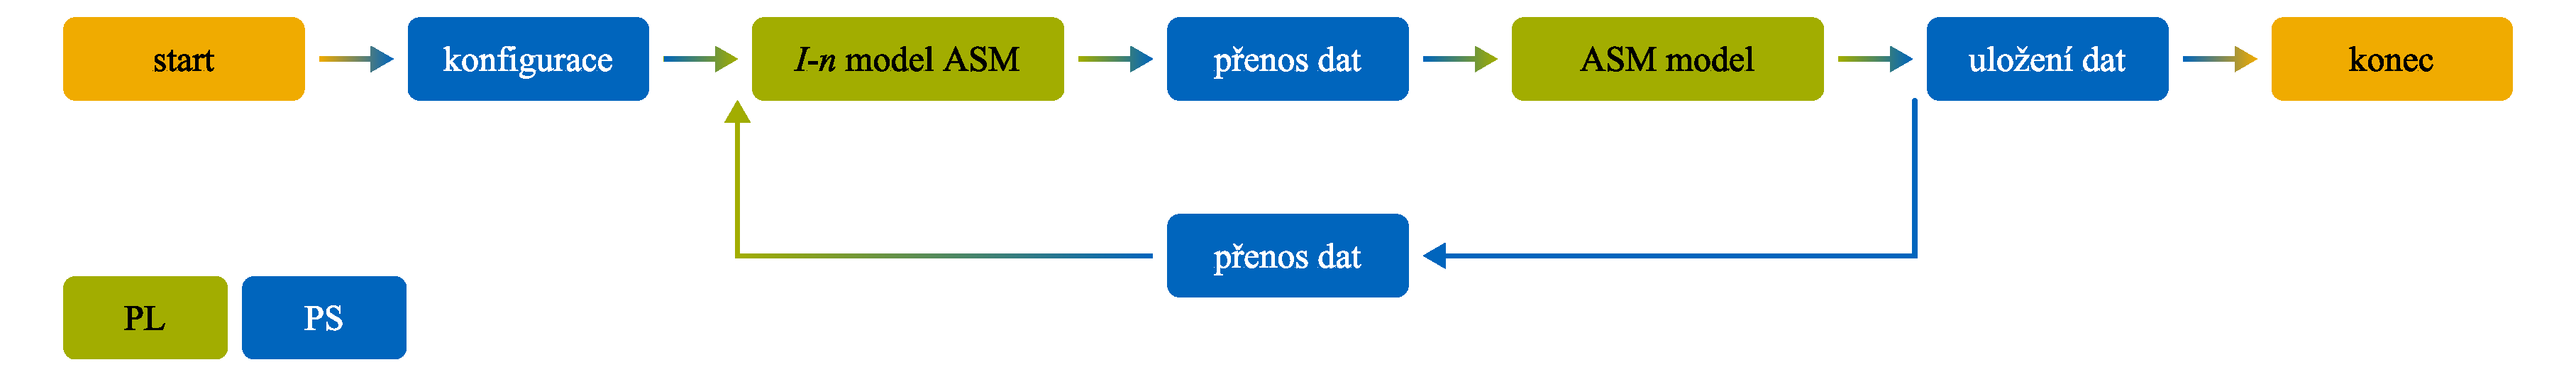
\includegraphics[width=1\textwidth]{src/pdf/rt-simulation-graph.pdf} 
					\caption{Graf prováděné simulace při testování PREEMPT\_\gls{abbreviation:rt} Linux Patch.}
					\label{fig:rt-simulation-graph}
			\end{figure}
			
			\fbar
			\subsubsection{Postup aplikace PREEMPT\_RT patch}\label{subsubsec:postup-aplikace-preempt-rt-patch}
				Patch je možné aplikovat několika způsoby. V~této práci byl aplikován při tvoření \textit{PetaLinux} systému pomocí úpravy konfiguračních souborů build procesu.\par
				Pro bezproblémové aplikování patche je vhodné nejdříve vytvořit \textit{build} \textit{PetaLinux} systému s~minimální konfigurací a bez aplikovanání patch souboru a až po úspěšném vytvoření systému patch aplikovat a build proces opakovat. Pro funkční aplikaci patch souboru je nutné znát verzi jádra \textit{PetaLinux}, na který bude aplikován. Označení verze je možné získat z~\texttt{Makefile} souboru umístěného v~cestě naznačené v~kódu \ref{lst:petalinux-kernel-makefile-path}, kde \texttt{<petalinux-project>} je označení pro kořenový (root) adresář \textit{PetaLinux} projektu.

				\begin{lstlisting}[language={sh}, caption={Cesta Makefile souboru, ze kterého je možné získat označení verze jádra systému PetaLinux.}, label= {lst:petalinux-kernel-makefile-path}]
<petalinux-project>/build/tmp/work-shared/xilinx-k26-kr/kernel-source/Makefile\end{lstlisting}
				Protože je zmiňovaný \texttt{Makefile} soubor rozsáhlý a pro určení verze kernelu je signifikantní pouze jeho úvodní část, je v~kódu č. \ref{lst:petalinux-makefile-kernel-version} vynechána podstatná část souboru, která není pro aplikování patche podstatná.

				\begin{lstlisting}[language={make}, caption={Významná část Makefile souboru pro určení verze jádra PetaLinux systému.}, label= {lst:petalinux-makefile-kernel-version}]
# SPDX-License-Identifier: GPL-2.0
VERSION = 5
PATCHLEVEL = 15
SUBLEVEL = 36
EXTRAVERSION =
NAME = Trick or Treat
...\end{lstlisting}
				
				Z~kódu \ref{lst:petalinux-makefile-kernel-version} je možné vyčíst, že je třeba využít patch pro verzi jádra \textit{5.15.36}. Pokud není v~souboru informace ohledně verze jádra linuxu uvedena, je možné vytvořit PetaLinux obvyklým způsobem, vytvořit obraz systému, ten nahrát na \gls{abbreviation:sd} kartu, provést spuštění systému na vývojové desce a po úspěšném přihlášení do systému vyvolat příkaz \texttt{uname -a} a dle uvedených informací odvodit verzi jádra.\par
				Poté je z~adresy \href{https://cdn.kernel.org/pub/linux/kernel/projects/rt}{\textcolor{ctublue}{https://cdn.kernel.org/pub/linux/kernel/projects/rt}} možné stáhnout patch pro zjištěnou verzi jádra. V~této práci byl využit patch jádra pro \textit{PetaLinux} 2022.2 umístěný v~cestě\\\texttt{5.15/older/patch-5.15.36-rt41.patch.gz}.\par
				Dalším krokem je extrahovaný soubor \texttt{patch-5.15.36-rt41.patch} přenést do složky\\\texttt{<petalinux-project>/project-spec/meta-user/recipes-kernel/linux/linux-xlnx/}. Build proces musí následně pracovat s~informací o~umístění patch souboru, proto je vyžadováno aby do konfiguračního souboru\\\texttt{<petalinux-project>/project-spec/meta-user/recipes-kernel/linux/linux-xlnx\_\%.bbappend} byl na poslední řádek zapsán příkaz\\\texttt{SRC\_URI:append = " file://patch-5.15.36-rt41.patch"},\\kde \texttt{patch-5.15.36-rt41.patch} je název patch souboru. Ukázka \texttt{linux-xlnx\_\%.bbappend} souboru, využitého v~této práci, je v~kódu \ref{lst:petalinux-patch-bbbappend}. Jak je vidět, soubor obsahuje informace o~různých konfiguračních souborech pro tvorbu jádra Linux systému.

				\begin{lstlisting}[language={sh}, caption={Ukázka konfiguračního souboru pro aplikování Linux patch souboru.}, label= {lst:petalinux-patch-bbbappend}]
FILESEXTRAPATHS:prepend := "${THISDIR}/${PN}:"

SRC_URI:append = " file://bsp.cfg"
KERNEL_FEATURES:append = " bsp.cfg"
SRC_URI:append = " file://patch-5.15.36-rt41.patch"
SRC_URI += "file://user_2023-04-07-11-32-00.cfg"\end{lstlisting}

				Aby došlo k~aplikování změn, vyvolaných \gls{abbreviation:rt} patch souborem, je nutné během build procesu provést určité změny v~konfiguraci vytvářeného \textit{PetaLinux} projektu. (postup předpokládá, že již byl vytvořen prvotní build s~minimální konfigurací) Opět jsou v~\textit{PetaLinux} Environment (prostředí) vyvolány příkazy \texttt{petalinux-config} pro prvotní konfiguraci \gls{abbreviation:hw} a \texttt{petalinux-confic -c kernel} pro konfiguraci jádra. Po otevření konfigurační nabídky jádra je nutné provést změny, vyznačené v~\ref{lst:kernel-config-rt-patch}.

				\begin{lstlisting}[language={sh}, caption={Úpravy v~konfiguraci jádra pro \gls{abbreviation:rt} patch.}, label= {lst:kernel-config-rt-patch}]
General setup -> Timers subsystem -> High Resolution Timer Support <*>
General setup -> Preemption Mode -> Fully Preemptive Kernel (RT) <*>
Main menu -> Kernel Features -> Timer frequenc -> 1000 Hz <*>
Main menu -> CPU power Management -> CPU Frequency Scaling < >\end{lstlisting}

				\noindent Značení:
				\begin{description}
					\item[] \texttt{< >} funkce není aktivována,
					\item[] \texttt{<*>} funkce je aktivována.
				\end{description}

				Po konfiguraci je již možné provádět build proces klasickým způsobem, popsaným v~části \hyperref[subsec:tvorba-petalinux]{\textit{Tvorba PetaLinux}}.\par
				Představený postup čerpá informace o~aplikování patch souboru z~\cite{hackster-real-time-optimization-in-petalinux-with-rt-patch-on-mpsoc}, \cite{trenz-electronic-wiki-how-to-install-the-linux-rt} a z~experimentálního zjištění autora.\par


			

		\subsection{Programovací prostředí – operační systém Linux}
			Pro práci s~představenými nástroji \hyperref[subsec:xilinx-vivado]{\textit{Xilinx Vivado}}, \hyperref[subsec:xilinx-vitis]{\textit{Xilinx Vitis}} a \hyperref[subsec:petalinux-tools]{\textit{PetaLinux Tools}} je nutné využívat podporovaných operačních systémů.\par
			Požadavky na operační systémy je možné nalézt na stránkách dokumentace \href{https://docs.xilinx.com}{\textcolor{ctublue}{https://docs.xilinx.com}}. V~době zpracování této práce jsou pro nejnovější verze nástrojů 2022.2 požadavky pro \hyperref[subsec:xilinx-vivado]{Xilinx Vivado} dostupné v~\cite{xilinx-vivado-design-suite-user-guide-2022}. Požadavky na operační systém pro \hyperref[subsec:xilinx-vitis]{Xilinx Vitis} v~\cite{vitis-unified-software-platform-documentation-2022}. Pro využivání a tvorbu \hyperref[subsec:petalinux-tools]{PetaLinux Tools} je třeba dodržet systémové požadavky uvedené v~\cite{petalinux-tools-documentation-2022}.\par
			Pokud uživatel využívá starších verzí vývojových nástrojů, je doporučeno využít operační systém Linux. Pro tuto práci byl nejdříve využíván systém Ubuntu 18.04 \gls{abbreviation:lts} (Bionic Beaver), dostupný ke stažení na adrese \href{http://old-releases.ubuntu.com}{\textcolor{ctublue}{http://old-releases.ubuntu.com}}. V~průběhu práce došlo k~aktualizování verzí vývojových nástrojů, které byly původně kompatibilní pouze s~verzí Ubuntu 18.04 a nižší. Veškerá práce a postupy byly po aktualizaci přeneseny na novější verzi systému Ubuntu 20.04 \gls{abbreviation:lts} (Focal Fossa).\par
			Je důležité poznamenat, že když Vivado podporuje některou z~novějších verzí Ubuntu, není jisté, že jí podporuje také \textit{PetaLinux Tools}. Vždy je doporučeno využívat starší verze a kontrolovat vzájemnou kompatibilitu, aby se předešlo zbytečné ztrátě času při reinstalací nástrojů.\par
			V~případě využívání představených nástrojů a systému Linux je třeba dbát na správné postupy instalací a v~případě problémů využívat dostupné dokumentace.
		% Jaké verze jsou momentálně podporované
		% Co je třeba nainstalovat za balíčky před započetím instalace
		% Jaký je flow aby byla možná příprava systému
		% Proč zrovna linux Open Source

	\section{Struktura složek}\label{sec:struktura-slozek}
		Aby byl vývoj, debugging, deployment a verzování aplikace co nejméně problematickým a zdlouhavým procesem pro vývojáře (jak \gls{abbreviation:hw} tak \gls{abbreviation:sw}), je vhodné zavést pro daný projekt pevný systém složek (file system), který bude dodržován napříč projekty. V~případě existence takového systému je možné vytvořit postupy a skripty, které značně urychlí práci na vyvíjeném projektu.\par
		Tyto skripty mohou sloužit ke~snadnějšímu přenosu souborů mezi jednotlivými složkami pro potřeby daných vývojových nástrojů, přenos souborů na vývojovou desku a nebo k~výrazně rychlejší práci s~vývojovými nástroji \textit{PetaLinux Tools} a Vitis \gls{abbreviation:ide}.
		V~této práci bude dodržována struktura naznačená v~kódu~\ref{lst:struktura-slozek}.

		\begin{lstlisting}[language={Text}, caption={Struktura složek, využívaná při tvorbě projektů k~dosažení lepšího \gls{abbreviation:dx}.}, label= {lst:struktura-slozek}]
- projects folder
	- top folder (project name)
		- transfer				// user generated
		- hw							// vivado project
		- petalinux				// petalinux project
		- linux-files			// user generated folders
			- pfm
				- boot
				- sd_dir
			- dtg_out				// created when converting device tree from XSA file
			- sysroots			// created by ./sdk.sh -d ./../linux-files
		- vitis\end{lstlisting}

		Tato struktura přináší možnosti rychlejšího pohybu v~projektu pomocí vzdáleného přístupu \gls{abbreviation:ssh} a emulátoru terminálu, který umožňuje provádět build aplikace i bez použití \gls{abbreviation:gui} Vitis \gls{abbreviation:ide}. Využíváním headless módu dochází k~odstranění některých nedostatků \gls{abbreviation:sw}. Ovšem \gls{abbreviation:gui} je vhodné na provádění úkonů, jejichž způsob provedení v~headless módu nebyl při realizaci této práce objeven (tvorba platformy, tvorba aplikace, automatické vytváření \texttt{makefile} souborů apod.).\par
		V~případě verzování projektu je ovšem důležité si uvědomit, že některé soubory mají značnou velikost a některé složky obsahují velmi mnoho souborů (více než 8 000 souborů). Proto je nutné tuto skutečnost vnímat a dle vlastních požadavků vyjmout vybrané prvky z~verzování.
		

	\section{Tvorba HW architektury Xilinx Vivado}
		Aby bylo možné vytvořit akcelerovanou aplikaci ve Vitis s~pomocí \gls{abbreviation:hls} C++, je třeba připravit platformu, resp. hardware, pro který bude daná aplikace vyvíjena. K~tvorbě platformy je využit Xilinx Vivado. V~tomto programu je možné konfigurovat jednotlivé \gls{abbreviation:ip} (intellectual property) prvky jako je ZynQ jednotka, \gls{abbreviation:gpio}, Timer, \gls{abbreviation:spi} komunikace a další. Výsledkem tvorby platformy v~této práci je soubor \gls{abbreviation:xsa}, který je použit pro konfiguraci \textit{PetaLinux} systému a slouží jako vstupní informace pro tvorbu Platformy ve Vitis. Ve Vivado je možné vytvářet aplikace přímo v~\gls{abbreviation:vhdl}.\par
		Tvorba \gls{abbreviation:hw} pro různé platformy (Digilent Zybo, Xilinx Kria KR260, \gls{abbreviation:soc}, \gls{abbreviation:som}) má částečně odlišné specifikace a odlišný postup. Rámcový postup je však totožný pro většinu platforem využívající zařízení od firmy Xilinx, Inc.\par
		V~této sekci bude popsána tvorba platformy pro vývojovou desku Xilinx Kria KR260 Starter Kit, na níž byla realizována finální aplikace. V~příloze práce je naznačen postup tvorby základní platformy pro vývojovou desku Digilent Zybo.\par

		\subsection{Vivado Board Files}\label{subsec:vivado-board-files}
			Aby bylo možné snadněji vytvořit potřebnou \gls{abbreviation:hw} architekturu, firmy často dodávají ke svému produktu \textit{Board Files} soubory, obsahující přednastavení, konfigurace, informace a způsob připojení \gls{abbreviation:ip} bloků k~reálným součástím (constraints). \cite{github-vivado-board-files-for-digilent-fpga-boards}\par
			Samozřejmě by bylo možné \gls{abbreviation:hw} architekturu vytvořit i bez těchto konfiguračních souborů, ovšem postup tvorby by byl značně náročnější. Pro vývojovou desku Xilinx Kria KR260 Starter Kit výrobce dodává Board files již s~instalací Vivado. Pro používanou vývojovou desku Digilent Zybo Zynq-7000 je možné stáhnout tyto soubory z~\cite{github-vivado-board-files-for-digilent-fpga-boards}. Způsob instalace board files je popsaný v~oficiální dokumentaci firmy Digilent, Inc. v~\cite{digilent-installing-vivado-vitis-and-digilent-board-files}.\par
			Po úspěšné instalaci souborů je možné spustit Xilinx Vivado a vytvořit potřebnou \gls{abbreviation:hw} architekturu pro akcelerovanou aplikaci.\par
			
		
		\subsection{Tvorba HW designu pro Xilinx Kria KR260 vývojovou desku}\label{subsec:tvorba-hw-designu-pro-xilinx-kria-kr260}
				Při tvorbě designu pro vývojovou desku Xilinx Kria KR260, byly čerpány základní rámcové informace o~postupu z~\cite{hackster-getting-started-with-the-kria-kr260-in-petalinux}, \cite{hackster-add-peripherial-support-to-kria-kr260-vivado} a \cite{hackster-getting-started-with-the-kria-kr260-in-vivado}. Konkrétní postup se liší dle vytvářené aplikace a zkoumaných vlastností.\par
				Protože prvotní zkoumání využitelnosti \gls{abbreviation:soc} bylo prováděno na desce Digilent Zybo Zynq-7000, je v~příloze \hyperref[sec:appendicies:-tvorba-hw-designu-pro-digilent-zybo-zynq-7000]{\textit{Tvorba HW designu pro Digilent Zybo Zynq-7000}} nastíněn postup tvorby \gls{abbreviation:hw} designu pro původní desku. Konfigurace \gls{abbreviation:ps} a tvorba \gls{abbreviation:hw} pro Digilent Zybo se odlišuje převážně proto, že Zybo používá starší \gls{abbreviation:ps} Zynq-7000, oproti novějšímu \gls{abbreviation:ps} MPSoC Zynq UltraScale+ v~Xilinx Kria.\par
				Prvním krokem je vytvoření Vivado projektu a jeho umístění do složky \texttt{hw} (popis struktury složek v~projektu je představen v~části \hyperref[sec:struktura-slozek]{\textit{Struktura složek}}).\par
				Postup tvorby projektu začíná pro většinu akcelerovaných aplikací stejným způsobem. Po otevření programu Vivado stačí vytvořit nový project typu \textit{\gls{abbreviation:rtl} Project} a aktivovat nastavení \textit{Project is an extensible Vitis platform}. Ukázka nabídky tvorby projektu je na obr.~\ref{fig:kr26-xilix-vivado-flow-01}.


				\begin{figure}[htbp!]
					\centering
					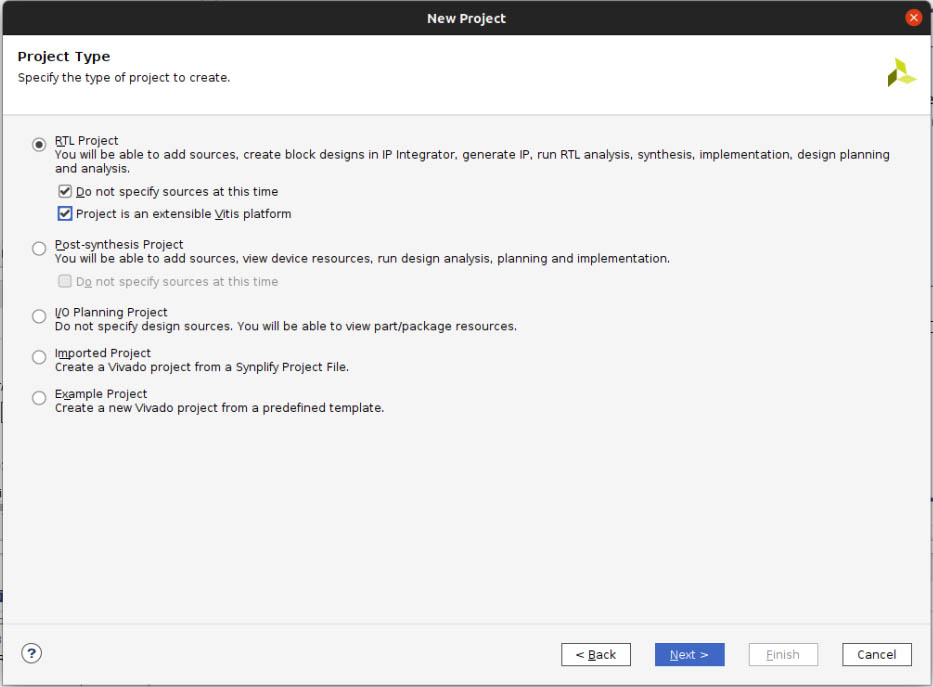
\includegraphics[width=0.85\textwidth]{src/png/kr26-xilinx-vivado-flow/kr26-xilix-vivado-flow-01.jpg}
					\caption{Xilinx Vivado – volba typu projektu pro Xilinx KR26, použitelného dále jako platforma ve Vitis.}
					\label{fig:kr26-xilix-vivado-flow-01}
				\end{figure}

				Dalším krokem při zakládání projektu je zvolení prvku, pro který bude vyvíjený \gls{abbreviation:hw} design určen. Je možné zvolit přímo komponentu, nebo již přednastavené vývojové desky. Pokud není vývojová deska v~repozitáři od Xilinx, je možné jí vložit dle způsobu popsaného v~části \hyperref[subsec:vivado-board-files]{\textit{Vivado Board Files}}. Xilinx Kria KR260 je však již součástí daného repozitáře a je možné ji v~repozitáři vyhledat a zvolit. Výběr desky z~repozitáře je zobrazen na obr. \ref{fig:kr26-xilix-vivado-flow-02}.

				\begin{figure}[htbp!]
					\centering
					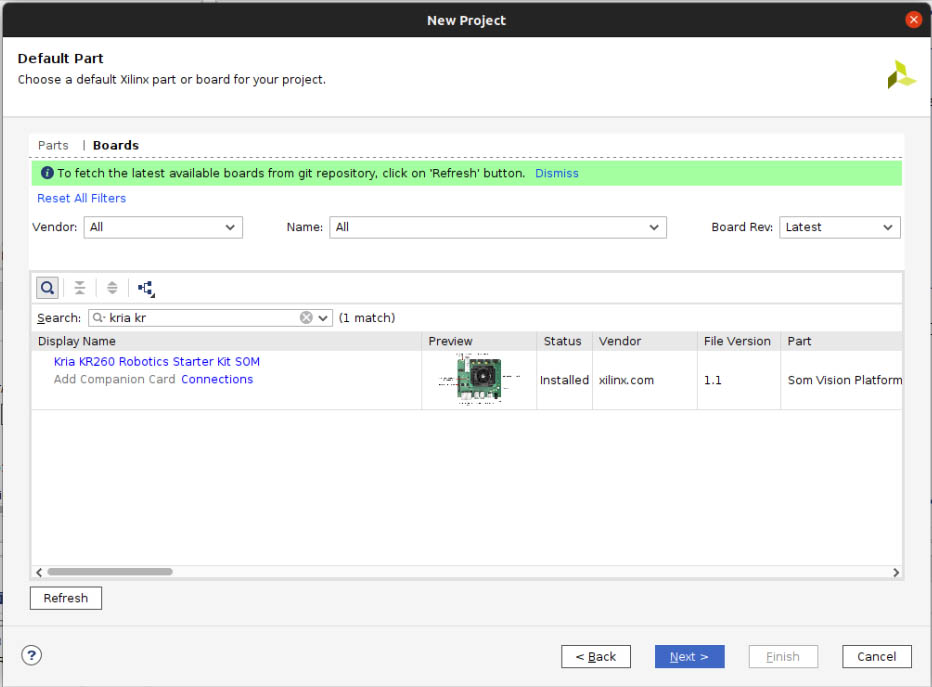
\includegraphics[width=0.85\textwidth]{src/png/kr26-xilinx-vivado-flow/kr26-xilix-vivado-flow-02.jpg}
					\caption{Xilinx Vivado – výběr základní komponenty, pro který bude \gls{abbreviation:hw} design vytvářen.}
					\label{fig:kr26-xilix-vivado-flow-02}
				\end{figure}

				Po vytvoření projektu je uživateli zobrazena hlavní Vivado obrazovka. V~základním nastavení jsou v~pravé části obrazovky zobrazeny informace o~vybrané základní komponentě/desce a v~levé části pracovní menu. Pro pokračování ve tvorbě designu je třeba zvolit v~menu odkaz \textit{Create block design} a pojmenovat jej dle požadavků autora designu. Menu a~nabídka vytváření blokového designu je zobrazena na obr.~\ref{fig:kr26-xilix-vivado-flow-03}.
		
				\begin{figure}[htbp!]
					\centering
					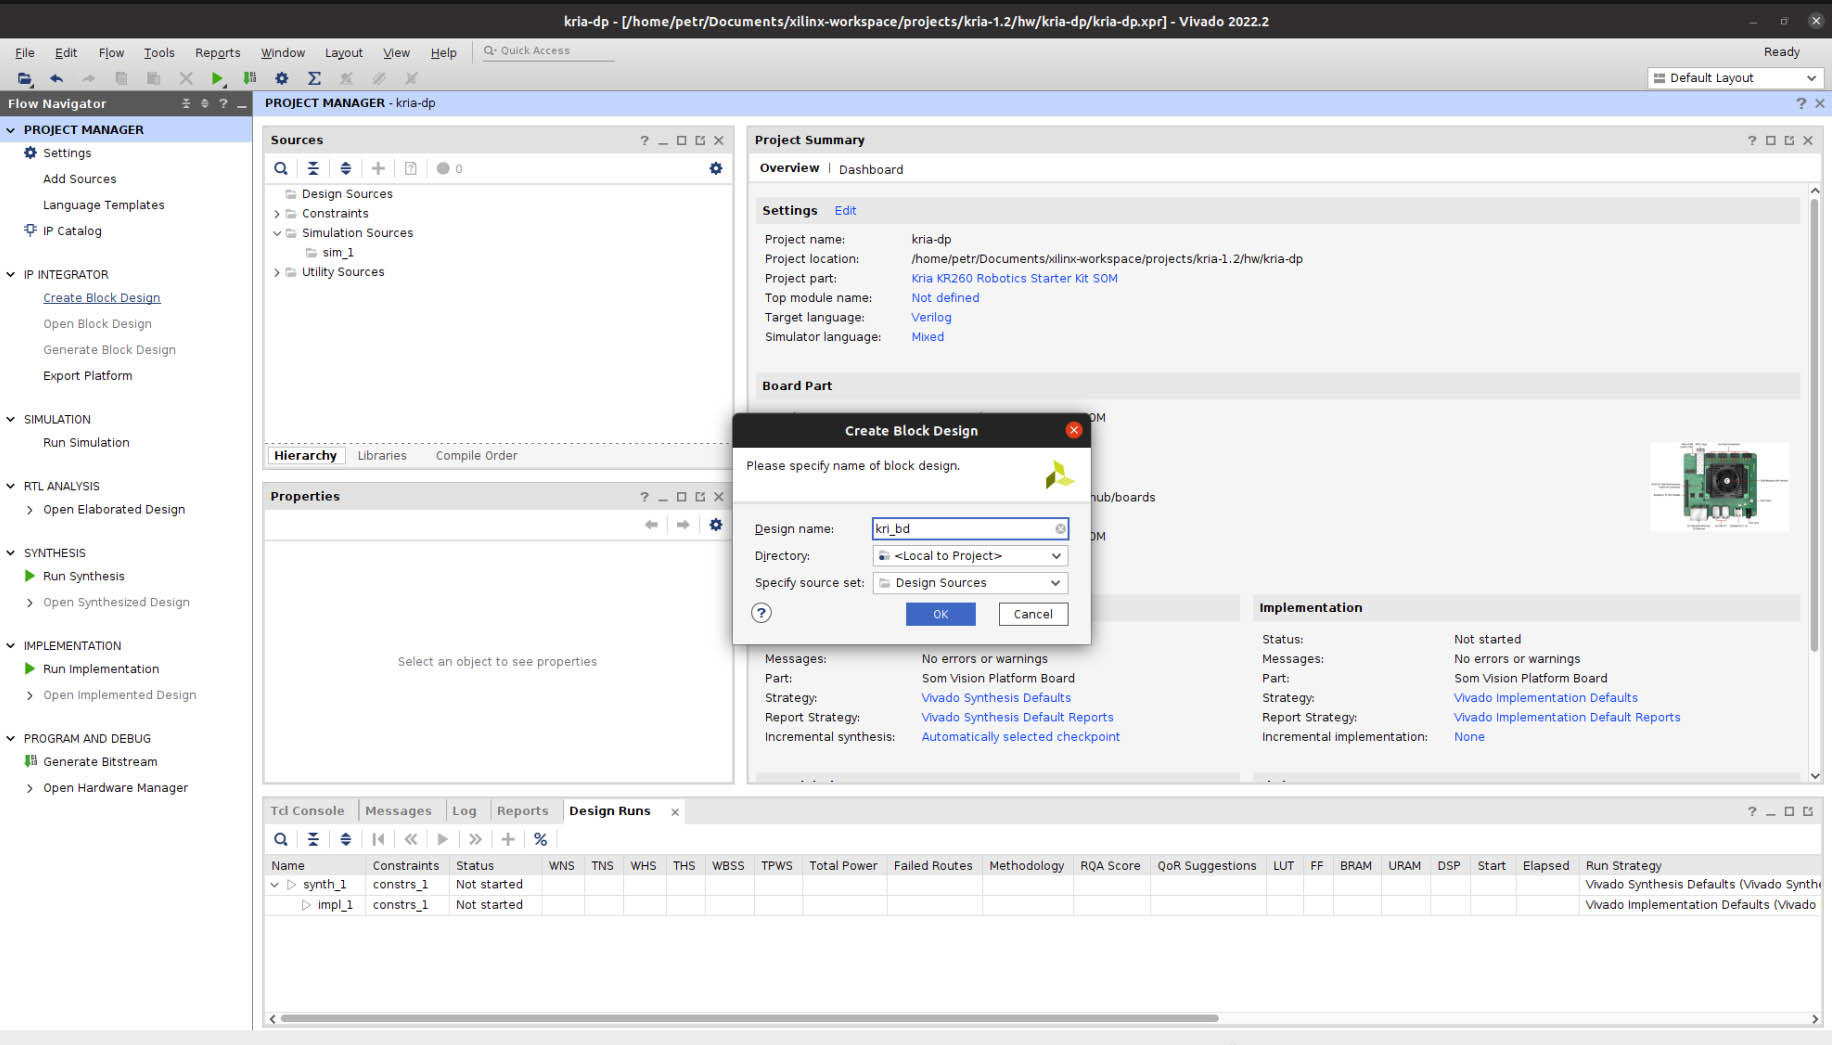
\includegraphics[width=1\textwidth]{src/png/kr26-xilinx-vivado-flow/kr26-xilix-vivado-flow-03.jpg}
					\caption{Xilinx Vivado – nabídka vytváření block design.}
					\label{fig:kr26-xilix-vivado-flow-03}
				\end{figure}

				Až po krok vytváření block designu byl postup velmi podobný pro obě představené vývojové desky. Nyní je již možné přistoupit k~vlastní tvorbě blokového designu v~kartě \textit{Diagram}.\par
				Bloky lze přidávat znakem „\texttt{+}“ v~aktivním okně nebo po kliknutí pravého tlačítka myši do volného prostoru v~téže okně a zvolení \textit{Add \gls{abbreviation:ip}}. Prvním krokem je přidání \gls{abbreviation:ps}, v~případě Xilinx KR26 se jedná o~\gls{abbreviation:ip} s~názvem \texttt{Zynq UltraScale+ MPSoC}. Výhoda používání Vivado je taková, že po vložení některých bloků je k~dispozici aktivace automatického propojení/nastavení některých bloků \gls{abbreviation:ip}. Po vložení \gls{abbreviation:ps} bloku je vhodné tuto automatizaci spustit pomocí aktivního odkazu, zobrazeného na kartě \textit{Diagram} v~obr. \ref{fig:kr26-xilix-vivado-flow-05}.

				\begin{figure}[htbp!]
					\centering
					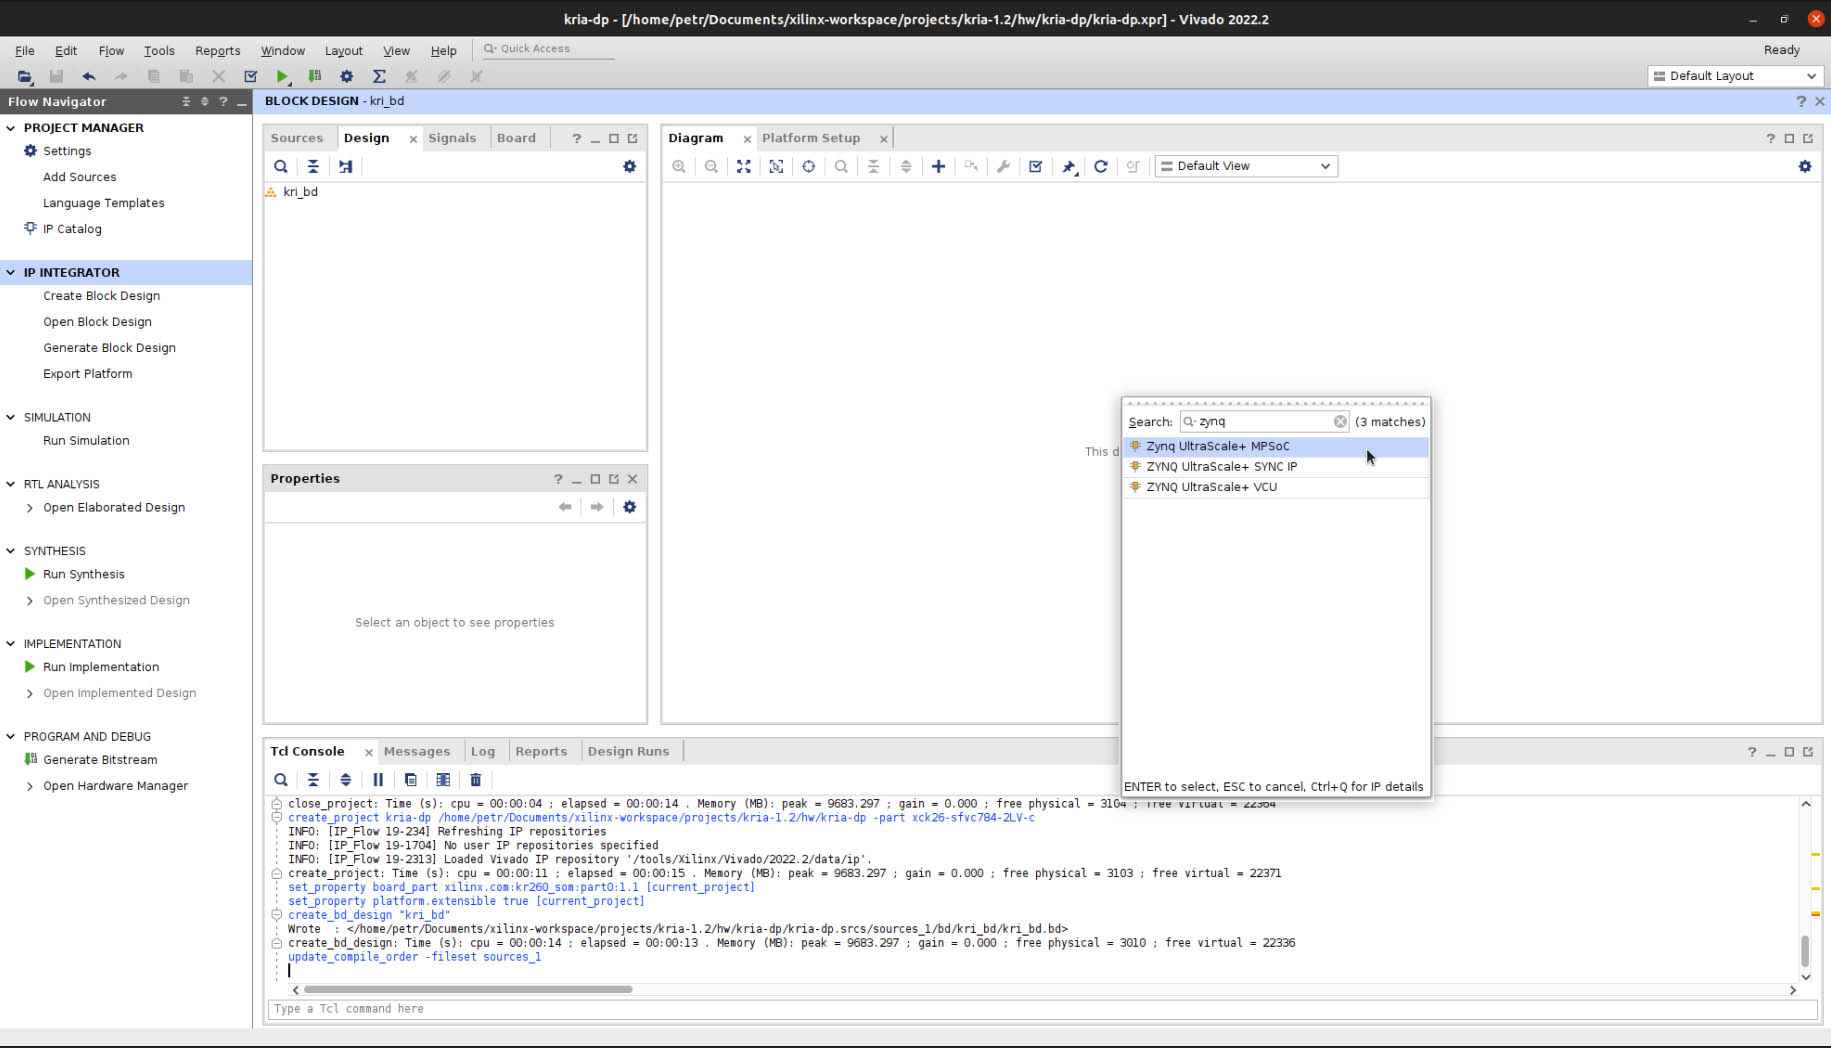
\includegraphics[width=1\textwidth]{src/png/kr26-xilinx-vivado-flow/kr26-xilix-vivado-flow-04.jpg}
					\caption{Xilinx Vivado – vložení \gls{abbreviation:ps} \gls{abbreviation:ip} bloku.}
					\label{fig:kr26-xilix-vivado-flow-04}
				\end{figure}

				\begin{figure}[htbp!]
					\centering
					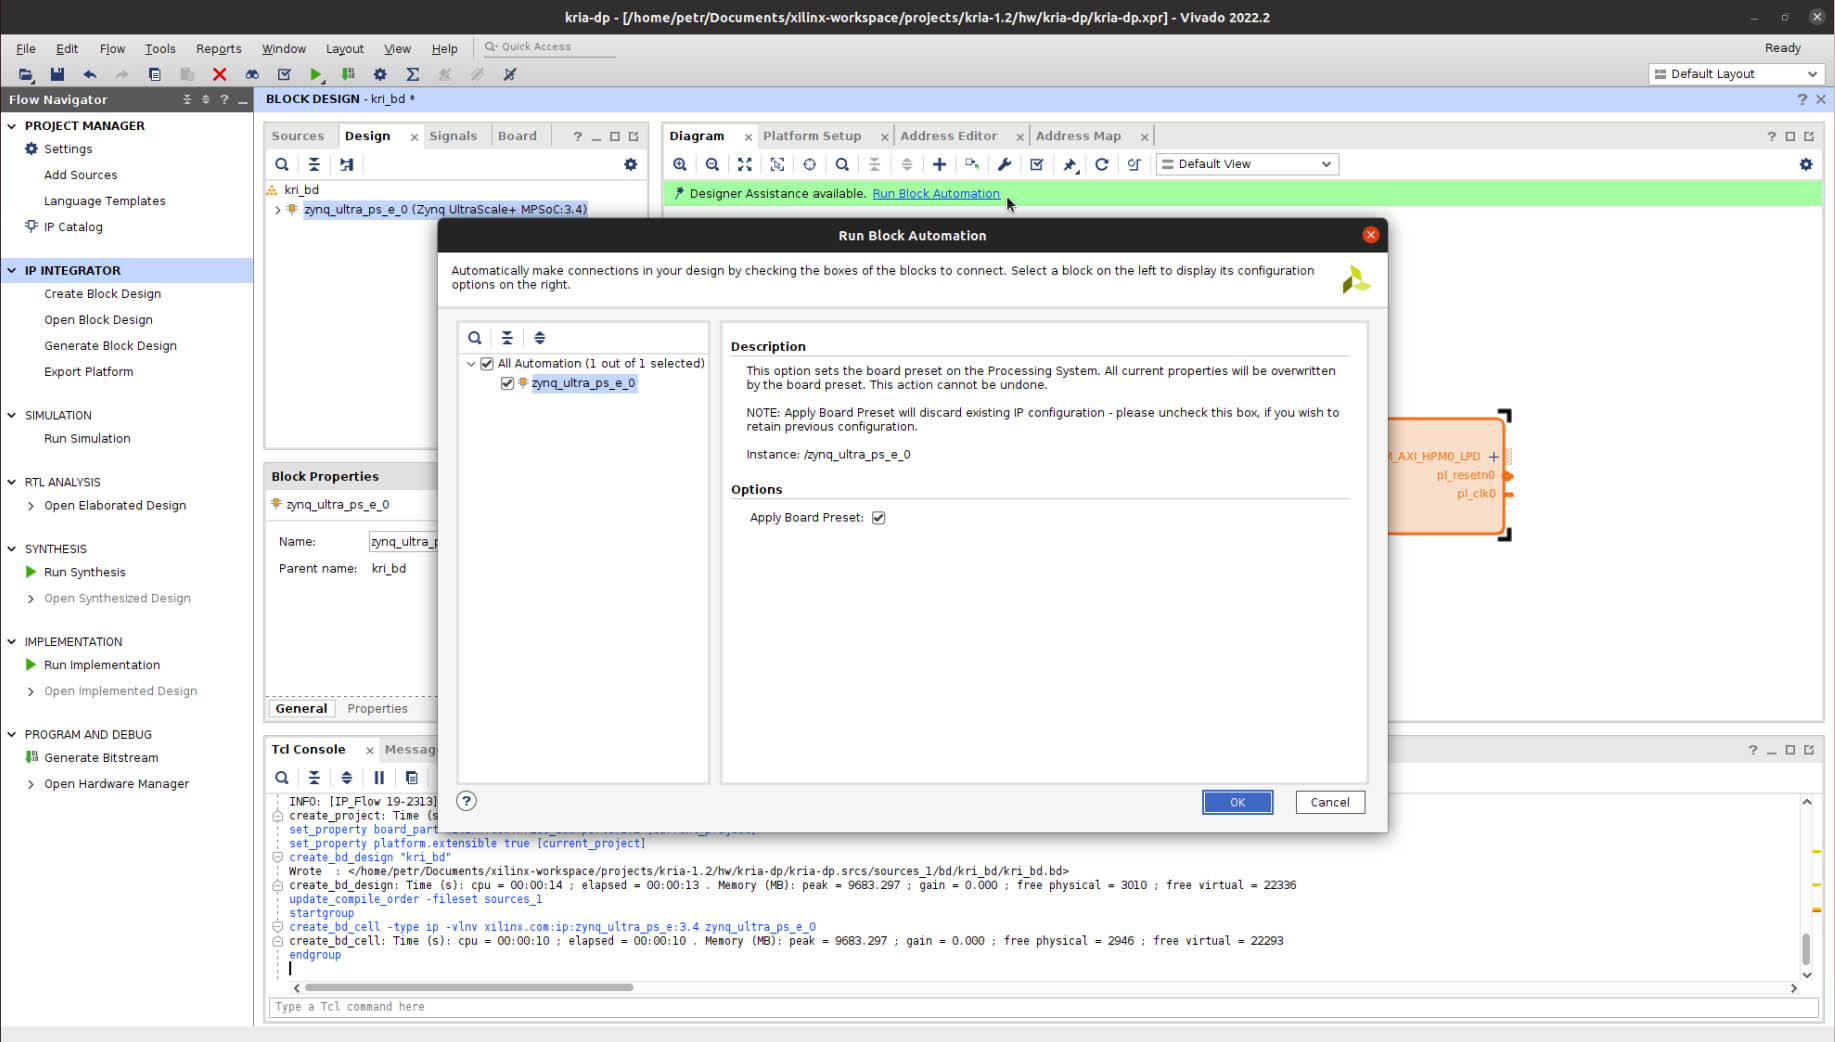
\includegraphics[width=1\textwidth]{src/png/kr26-xilinx-vivado-flow/kr26-xilix-vivado-flow-05.jpg}
					\caption{Xilinx Vivado – automatické propojení pro \gls{abbreviation:ps}.}
					\label{fig:kr26-xilix-vivado-flow-05}
				\end{figure}
				\fbar

				Další krok je důležitý pro tvorbu akcelerované aplikace pomocí Vitis. Je třeba předkonfigurovat \gls{abbreviation:ps} \gls{abbreviation:axi} (rozhraní) takovým způsobem, aby \gls{abbreviation:axi} s~vysokým výkonem bylo využito až pro akcelerovanou aplikaci a nikoliv v~některém z~automatických propojení, jejichž pozitivní přínos byl představen v~předchozím odstavci. Tato informace je popsána v~\cite{hackster-getting-started-with-the-kria-kr260-in-vivado} ale také v~oficiálních repozitářích \cite{xilinx-github-vitis-tutorials-step-1-create-the-vivado-hardware-design-and-generate-xsa} (\textit{v sekci Add Interrupt Support, krok 1}) pro tvorbu platformy vývojové desky Xilinx Kria KV260, jež používá totožný modul Xilinx Kria K26. Obr. \ref{fig:kr26-xilix-vivado-flow-06} obsahuje ukázku nastavení bloku \texttt{Zynq UltraScale+ MPSoC} a daných rozhraní.

				\begin{figure}[htbp!]
					\centering
					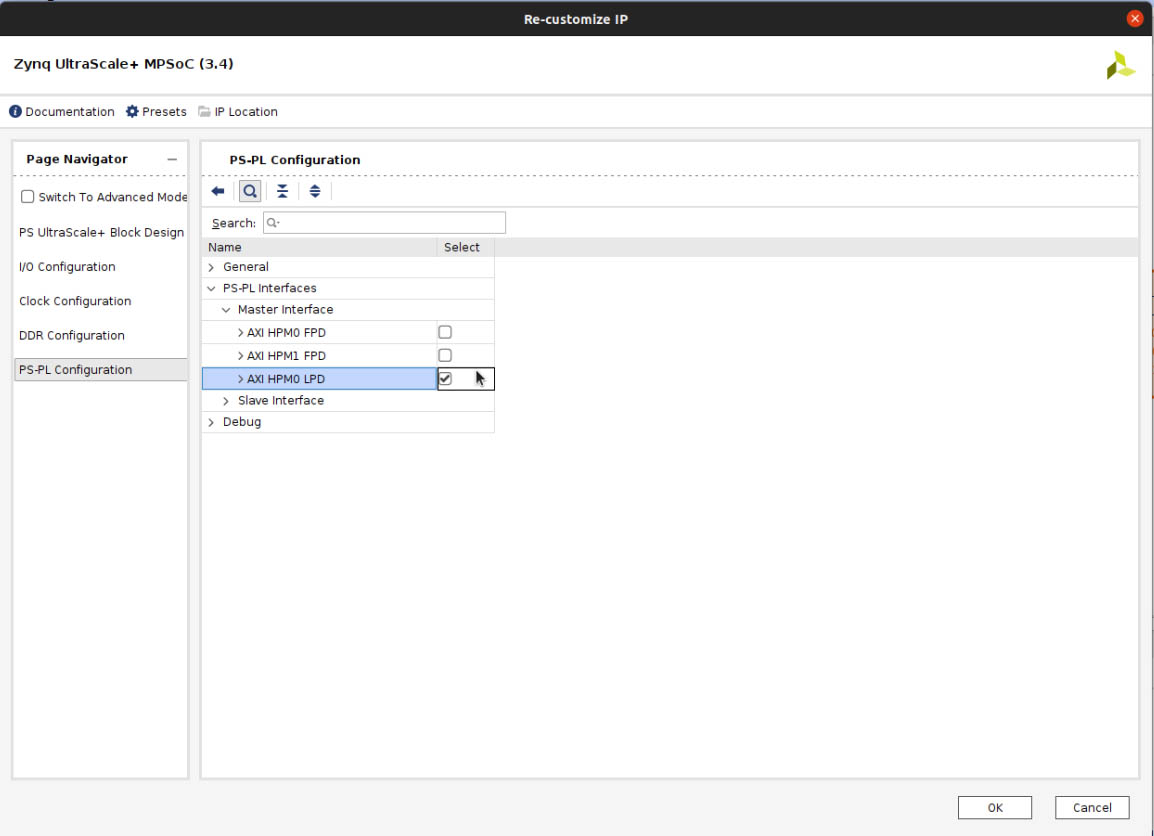
\includegraphics[width=0.85\textwidth]{src/png/kr26-xilinx-vivado-flow/kr26-xilix-vivado-flow-06.jpg}
					\caption{Xilinx Vivado – zablokování \gls{abbreviation:fpd} a odblokování \gls{abbreviation:lpd} pro block design.}
					\label{fig:kr26-xilix-vivado-flow-06}
				\end{figure}

				Protože dle \cite{xilinx-github-vitis-tutorials-step-1-create-the-vivado-hardware-design-and-generate-xsa} je počet clock signálů \texttt{pl\_clk} z~\gls{abbreviation:ps} omezený, je vhodné pro vytvoření požadovaných taktovacích signálů (pro \gls{abbreviation:pl}) využít blok \texttt{Clocking wizard}. V~tomto bloku je možné vytvořit taktovací signály s~požadovanými parametry. Pokud počet signálů nestačí, je možné přidat další \gls{abbreviation:ip}.\par
				Pro design ukázkové platformy v~této práci jsou využity tři taktovací signály s~frekvencí 100, 200 a 20 MHz. Také je důležité nastavit \textit{Reset type} na \textit{Active Low}. Příklad nastavení bloku \texttt{Clocking wizard} je na obr. \ref{fig:kr26-xilix-vivado-flow-07}.\par

				\begin{figure}[htbp!]
					\centering
					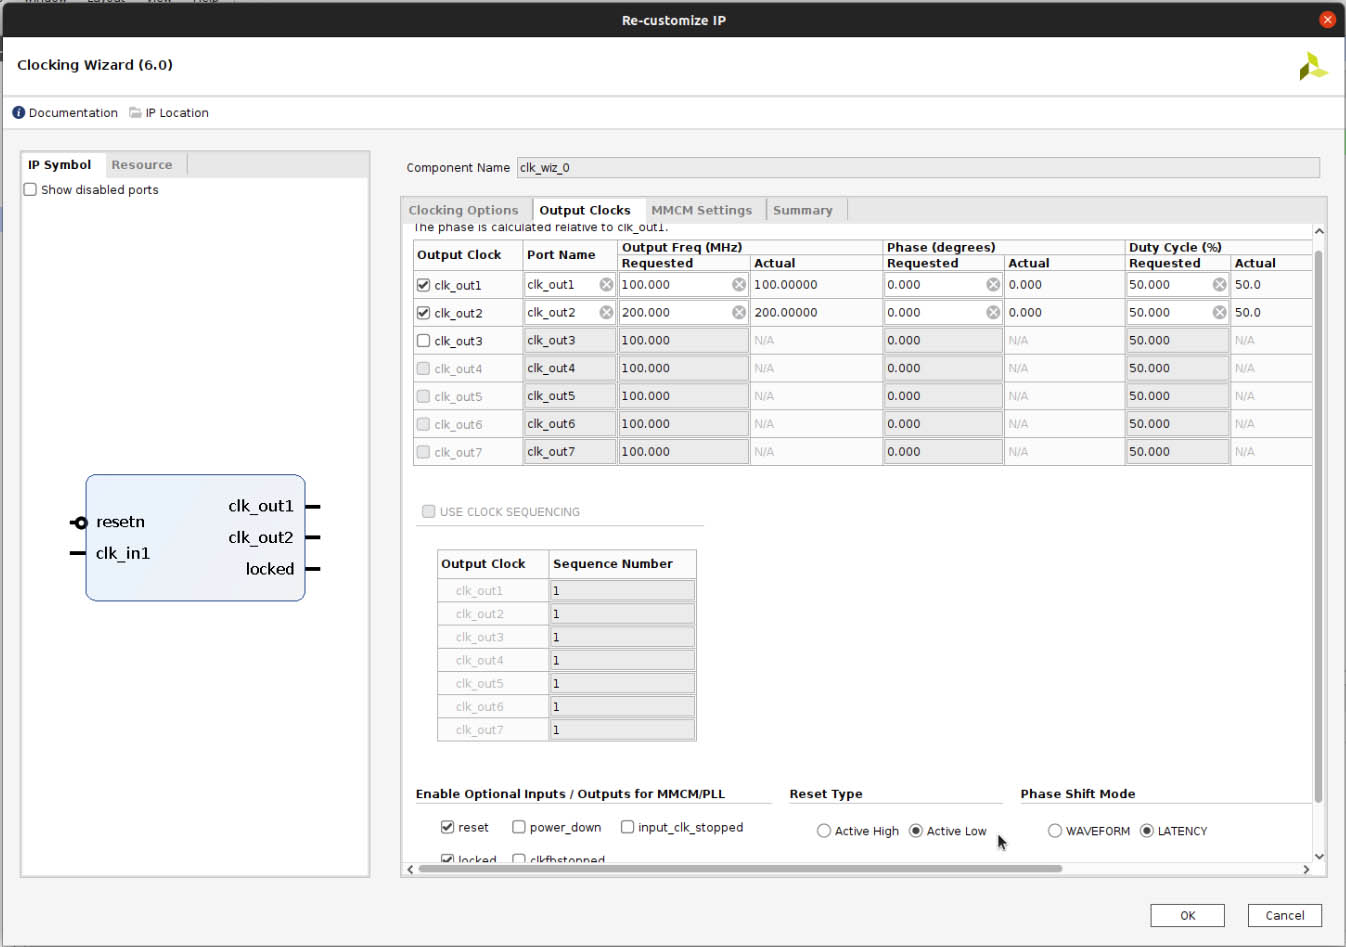
\includegraphics[width=0.85\textwidth]{src/png/kr26-xilinx-vivado-flow/kr26-xilix-vivado-flow-07.jpg}
					\caption{Xilinx Vivado – nastavení bloku Clocking wizard.}
					\label{fig:kr26-xilix-vivado-flow-07}
				\end{figure}
				Po nastavení požadovaných taktovacích signálů je možné opět pomocí aktivního odkazu automatizace spustit automatické propojení bloků. Po úspěšném provedení předchozích konfiguračních kroků a~automatizace je získáno schéma blokového designu na obr. \ref{fig:kr26-xilix-vivado-flow-08}.

				\begin{figure}[htbp!]
					\centering
					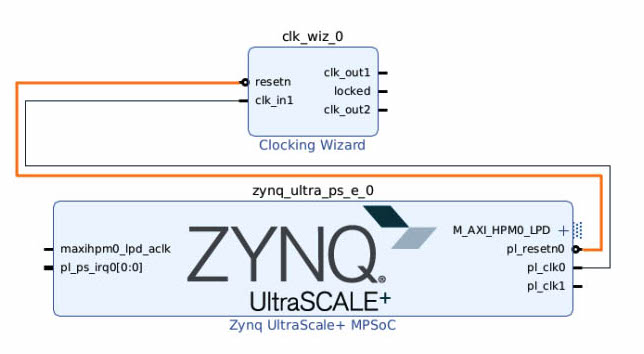
\includegraphics[width=0.85\textwidth]{src/png/kr26-xilinx-vivado-flow/kr26-xilix-vivado-flow-08.jpg}
					\caption{Xilinx Vivado – blokový design s~\gls{abbreviation:ps} a blokem Clocking wizard po provedení automatizace.}
					\label{fig:kr26-xilix-vivado-flow-08}
				\end{figure}

				K~bloku \texttt{Clocking Wizard} je nyní vhodné připojit bloky \texttt{Processor System Reset} dle obr. \ref{fig:kr26-xilix-vivado-flow-09}.

				\begin{figure}[htbp!]
					\centering
					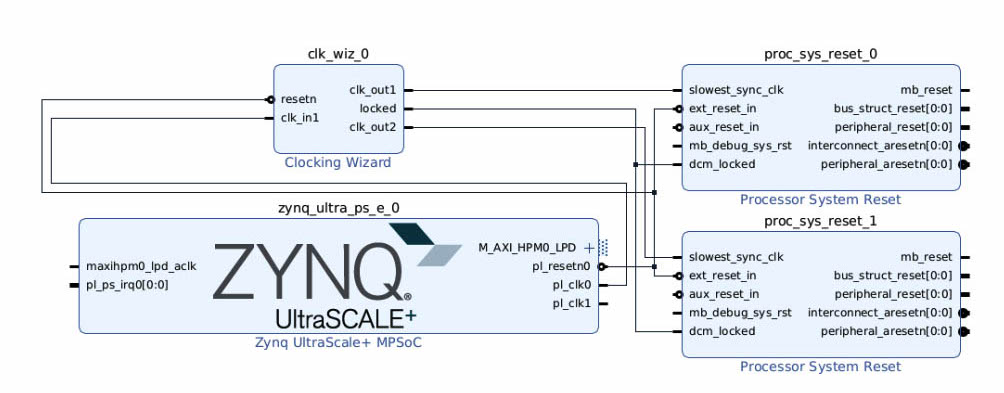
\includegraphics[width=0.95\textwidth]{src/png/kr26-xilinx-vivado-flow/kr26-xilix-vivado-flow-09.jpg}
					\caption{Xilinx Vivado – propojení bloků Clocking wizard a Processor System Reset.}
					\label{fig:kr26-xilix-vivado-flow-09}
				\end{figure}
				
				Vstup pro přerušení \texttt{pl\_ps irq} může obsahovat maximálně 16 interrupt signálů. Pro design v~této aplikaci se jedná o~dostačující počet, ovšem pokud je vyžadováno, aby aplikace využívala více signálů přerušení, je třeba využít blok \texttt{\gls{abbreviation:axi} Interrupt Controller}. Doporučené nastavení tohoto \gls{abbreviation:ip} je uvedeno na obr. \ref{fig:kr26-xilix-vivado-flow-10}. Aby bylo možné připojit signál k~\texttt{pl\_ps irq} je nutné přepnout nastavení \textit{Processor Interrupt Type and Connection -> Interrupt Output Connection} na \texttt{Single} z~výchozího \texttt{Bus}.\par
				V~případě nevyužití bloku \texttt{\gls{abbreviation:axi} Interrupt Controller}, nebo při snaze přivést signály přerušení přímo do \texttt{pl\_ps irq} vstupu \gls{abbreviation:ps} systému, je pro připojení více signálů doporučeno použít \gls{abbreviation:ip} blok \texttt{Concat}. V~dalších částech této práci je tento blok také využit, aby byla demonstrována možnost jeho využití a projevení tohoto připojení v~\textit{PetaLinux} systému.\par
				Po dokončení konfigurace \texttt{\gls{abbreviation:axi} Interrupt Controller} je možné aktivovat automatizaci propojení a v~konfiguračním okně vybrat požadovanou frekvenci \gls{abbreviation:clk} signálů. V~této práci je využito 200~MHz. Výsledný design po automatizaci je zobrazen na obr. \ref{fig:kr26-xilix-vivado-flow-12}.\par

				\begin{figure}[htbp!]
					\centering
					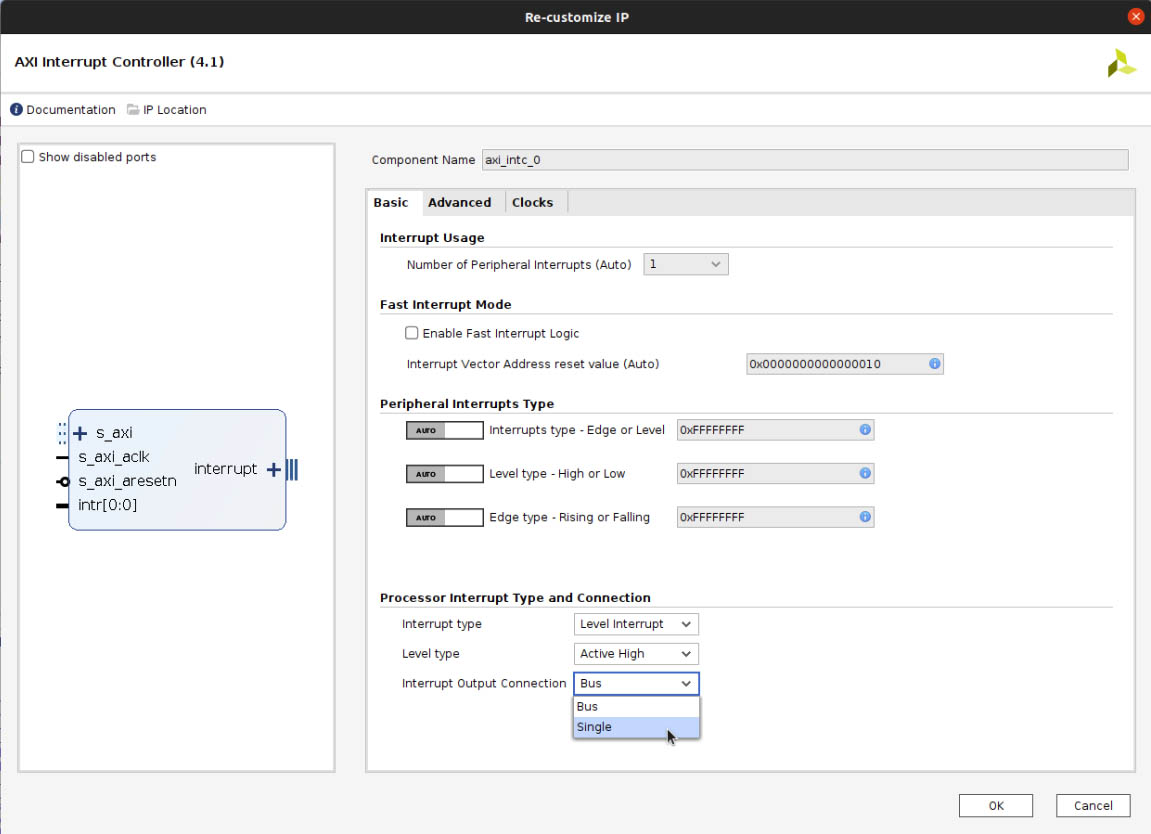
\includegraphics[width=0.85\textwidth]{src/png/kr26-xilinx-vivado-flow/kr26-xilix-vivado-flow-10.jpg}
					\caption{Xilinx Vivado – nastavení bloku \gls{abbreviation:axi} Interrupt Controller.}
					\label{fig:kr26-xilix-vivado-flow-10}
				\end{figure}

				\begin{figure}[htbp!]
					\centering
					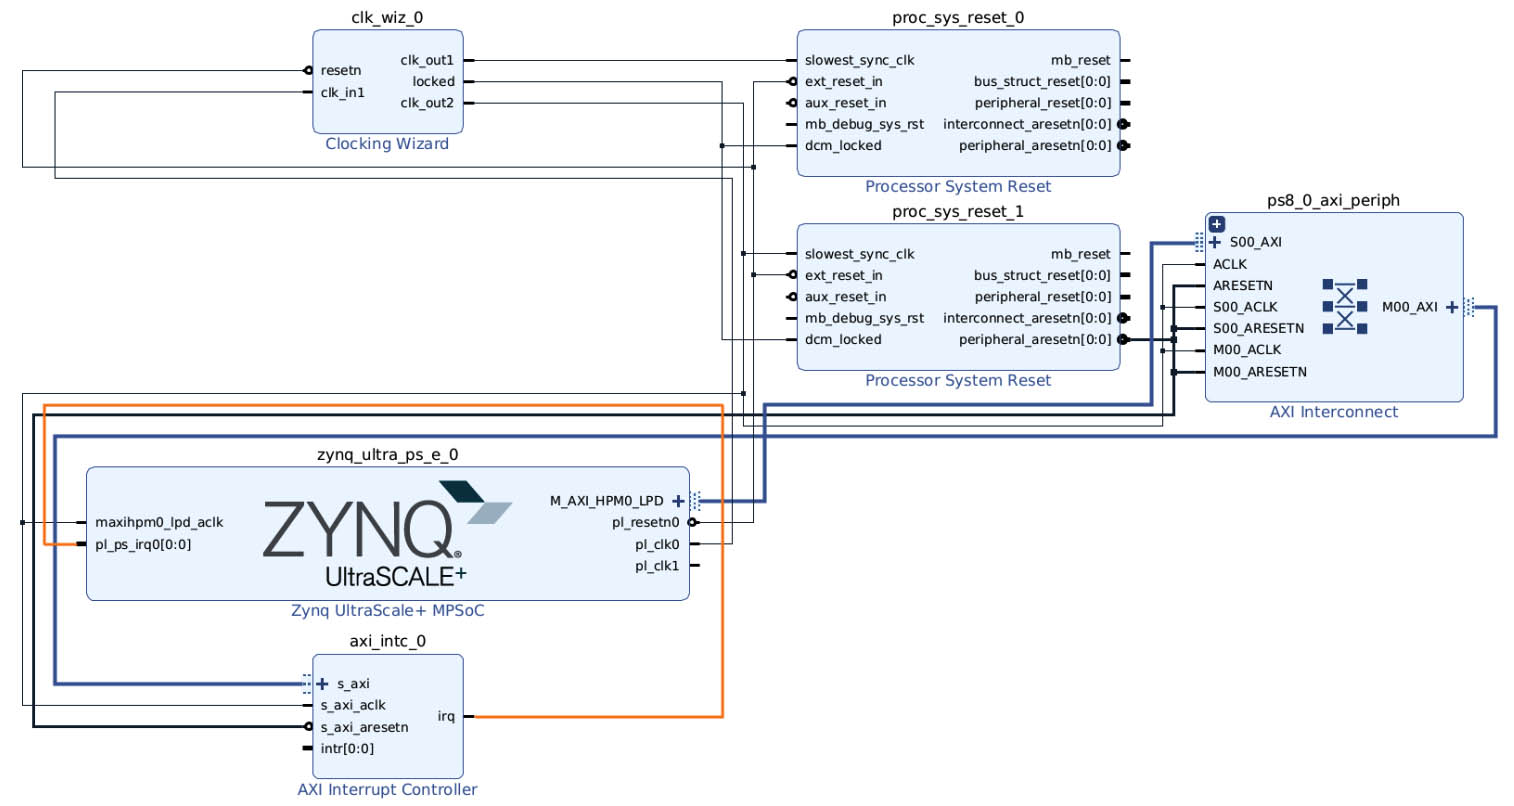
\includegraphics[width=1\textwidth]{src/png/kr26-xilinx-vivado-flow/kr26-xilix-vivado-flow-12.jpg}
					\caption{Xilinx Vivado – block design po automatizaci a propojení bloku \gls{abbreviation:axi} Interrupt Controller.}
					\label{fig:kr26-xilix-vivado-flow-12}
				\end{figure}
				\fbar
				Pokud by vyvíjená aplikace nevyužívala další \gls{abbreviation:pl} \gls{abbreviation:ip} bloky, je možné přistoupit ke konfiguraci platformy, \gls{abbreviation:ps} a periferií připojených k~\gls{abbreviation:ps}. Pro vyvíjenou ukázkovou aplikaci je vytvořený \gls{abbreviation:hw} blokový design naznačen v~sekci \hyperref[subsubsec:hw-block-design-vyvijene-aplikace]{\textit{HW Block design vyvíjené aplikace}}.\par
				Ovšem při využití vývojové desky Xilinx Kria KR260 je vhodné aktivovat řízení chladícího ventilátoru pomocí \gls{abbreviation:pwm}. Pro tuto možnost musí být aktivovaný výstup \textit{Waveout} u~TTC 0, jak je tomu naznačeno na obr. \ref{fig:kr26-xilix-vivado-flow-30}. Po aktivaci \textit{Waveout} na \gls{abbreviation:io} \textit{EMI0} se objeví na bloku \texttt{Zynq UltraScale+ MPSoC} výstup s~názvem \texttt{emio\_ttc0\_wave\_o[2:0]}. Označení \texttt{[2:0]} znamená, že signál je tříbitový. Pro řízení ventilátoru pomocí \gls{abbreviation:pwm} je ovšem využíván pouze jeden bit. Pro odstranění dvou horních bitů je využito \gls{abbreviation:ip} bloku \texttt{Slice}.\par
				Konfigurace bloku \texttt{Slice} je zobrazena na obr. \ref{fig:kr26-xilix-vivado-flow-29}. \textit{Din Width} určuje šířku vstupujícího signálu. V~řešeném případě se jedná o~tříbitový vstupní signál. \textit{Din From} určuje označení bitu, od kterého bude odstraněno \textit{Din Down To} bitů pro výstup z~bloku \texttt{Slice}. Vstup \textit{Dout Width} je automaticky doplněn dle nastavení předchozích položek.\par
				Následně je nutné nastavit výstupní pin, na který bude signál \gls{abbreviation:pwm} pro řízení ventilátoru odesílán. Pro vytvoření pinu existuje mnoho způsobů, v~tomto případě je ovšem nejjednodušší pravým tlačítkem myší kliknout na výstup bloku \texttt{Slice} \texttt{Dout[0:0]} a zvolit \textit{Make External}. Tento pin je poté vhodné pojmenovat \texttt{fan\_en\_b}. Minimální funkční design s~výstupním pinem pro ventilátor je zobrazen na obr.~\ref{fig:kr26-xilix-vivado-flow-31}.

				\begin{figure}[htbp!]
					\centering
					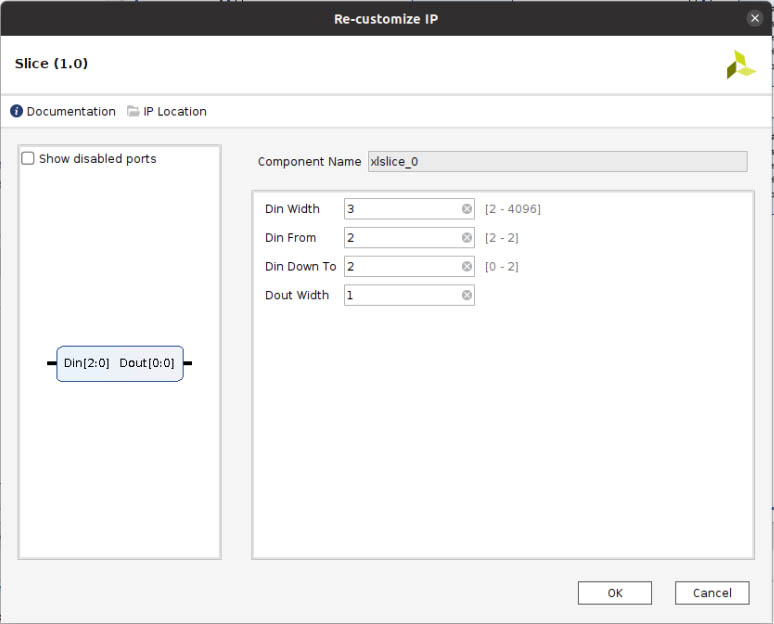
\includegraphics[width=0.85\textwidth]{src/png/kr26-xilinx-vivado-flow/kr26-xilix-vivado-flow-29.jpg}
					\caption{Xilinx Vivado – nastavení bloku Slice pro odstranění dvou horních bitů signálu.}
					\label{fig:kr26-xilix-vivado-flow-29}
				\end{figure}

				\begin{figure}[htbp!]
					\centering
					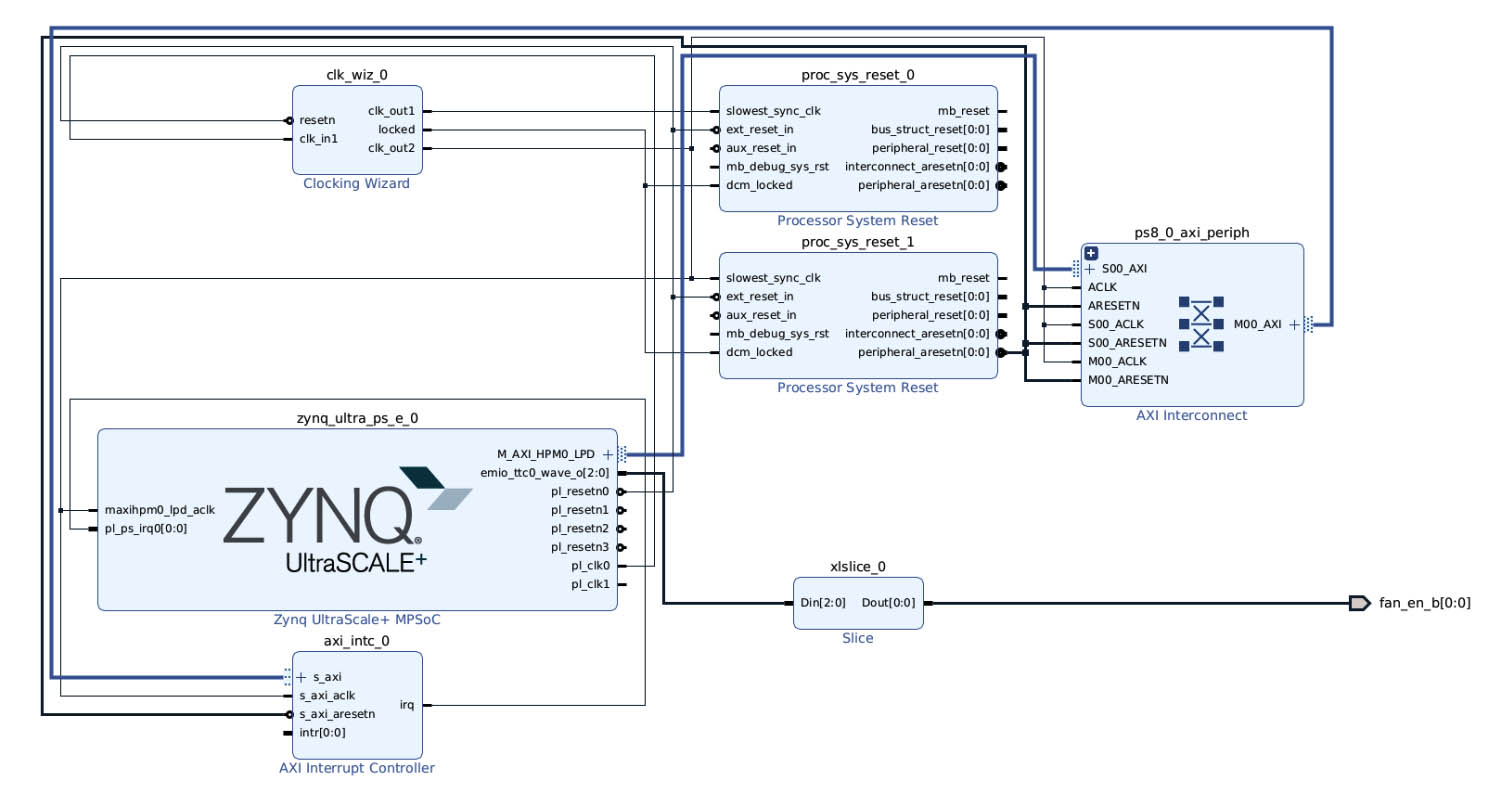
\includegraphics[width=1\textwidth]{src/png/kr26-xilinx-vivado-flow/kr26-xilix-vivado-flow-31.jpg}
					\caption{Xilinx Vivado – minimální funkční design s~výstupním pinem pro řízení ventilátoru.}
					\label{fig:kr26-xilix-vivado-flow-31}
				\end{figure}


				Na kartě \textit{Platform Setup} je pro funkční design vhodné aktivovat a pojmenovat základní \gls{abbreviation:axi} porty dle tabulky \ref{tab:vivado-platform-setup-axi-xilinx-kria}.


				\begin{table}[H]
					\centering
					\caption{Ukázka nastavených \gls{abbreviation:axi} portů v~Xilinx Vivado platformě pro Xilinx Kria KR260.}
				  \vspace*{0.15cm}
				
					\begin{tabular}{!{\vrule width 2pt} c | c | c | c !{\vrule width 2pt}}
					\noalign{\hrule height 2pt}
					\rowcolor{codeblue}
					Name & Enabled & Memport & SP Tag\\
					\noalign{\hrule height 2pt}
					M\_AXI\_HPM0\_FPD & X & M\_AXI\_GP & -\\ \hline
					M\_AXI\_HPM1\_FPD & X & M\_AXI\_GP & -\\ \hline
					S\_AXI\_HPC0\_FPD & X & S\_AXI\_HPC & HPC0\\ \hline
					S\_AXI\_HPC1\_FPD & X & S\_AXI\_HPC & HPC1\\ \hline
					S\_AXI\_HP0\_FPD & X & S\_AXI\_HP & HP0\\ \hline
					S\_AXI\_HP1\_FPD & X & S\_AXI\_HP & HP1\\ \hline
					S\_AXI\_HP2\_FPD & X & S\_AXI\_HP & HP2\\ \hline
					S\_AXI\_HP3\_FPD & X & S\_AXI\_HP & HP3\\ \noalign{\hrule height 2pt}
					\end{tabular}
					\label{tab:vivado-platform-setup-axi-xilinx-kria}
				\end{table}

				Dalším krokem je povolení a nastavení výchozích \gls{abbreviation:clk} signálů v~záložce \textit{Clock}. V~této práci byl zvolen výchozí \gls{abbreviation:clk} signál 200 MHz. Snímek záložky zachycující nastavení pro dva clock signály je na obr. \ref{fig:kr26-xilix-vivado-flow-14}.\par
				Posledním důležitým krokem je v~kartě \textit{Platform Setup -> Interrupt} povolit signál \texttt{intr} z~použitého bloku \texttt{Axi Interrupt Controller}.\par
				Volitelným, ovšem vhodným krokem je pojmenovat platformu a udat jejího autora a verzi v~kartě \textit{Platform Setup -> Interrupt}.

				\begin{figure}[htbp!]
					\centering
					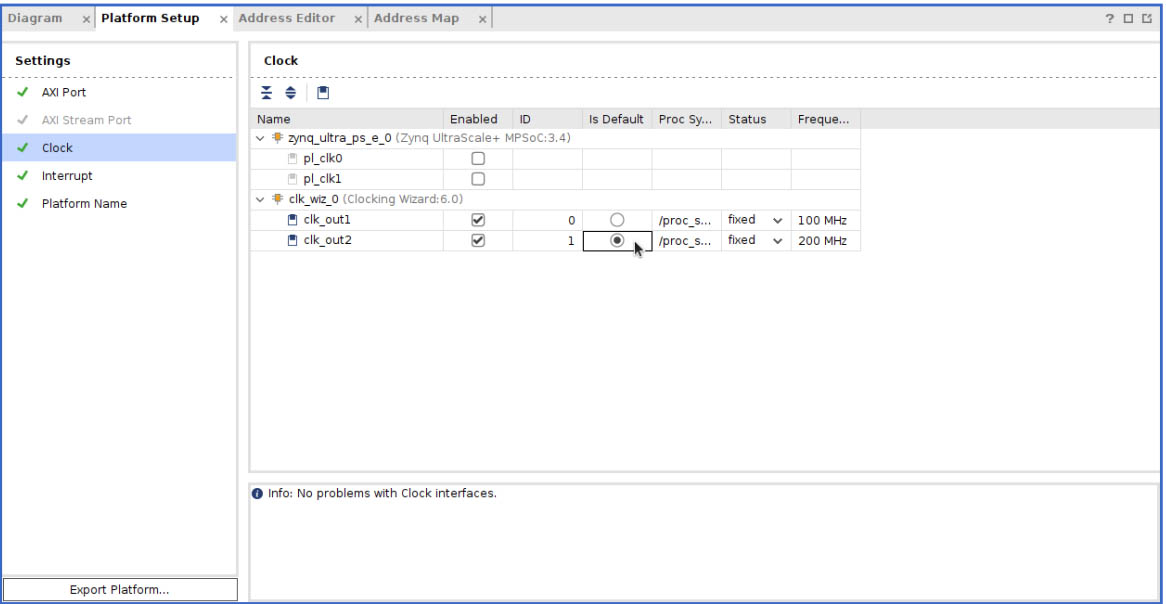
\includegraphics[width=0.95\textwidth]{src/png/kr26-xilinx-vivado-flow/kr26-xilix-vivado-flow-14.jpg}
					\caption{Xilinx Vivado – záložka nastavení \gls{abbreviation:clk} signálů na platformě.}
					\label{fig:kr26-xilix-vivado-flow-14}
				\end{figure}


				Autorka článku \cite{hackster-getting-started-with-the-kria-kr260-in-vivado} zmiňuje, že pokud je zapnuta možnost \textit{Incremental Synthesis}, můžou vznikat při postupu tvorby akcelerované aplikace problémy. Proto doporučuje pomocí nabídky \textit{Settings -> Synthesis -> Incremental Synthesis} zvolit možnost \textit{Disable incremental synthesis}.\par

				\subsubsection{Konfigurace PS pro využití implementovaných periferií}
				Aby bylo možné využívat periferie, jako je DisplayPort, Ethernet nebo \gls{abbreviation:usb} konektory, je nutné nakonfigurovat \gls{abbreviation:ps}. Konfigurační nabídka je otevřena při konfiguraci \gls{abbreviation:ip} bloku \texttt{Zynq UltraScale+ MPSoC} a vybrání \textit{\gls{abbreviation:io} Configuration}.\par
				Pro názornost je využito snímků obrazovky jednotlivých významných konfigurací. Některé z~konfigurací jsou již nastaveny jako výchozí, některé je třeba konfigurovat.\par
				Na obr. \ref{fig:kr26-xilix-vivado-flow-17} je zobrazeno kompletní konfigurační okno ve kterém jsou jednotlivá připojení pro \gls{abbreviation:ps} nastavovány. Další snímky jsou však z~důvodu úspory plochy zaměřeny pouze na konkrétní nastavení.

				\begin{figure}[htbp!]
					\centering
					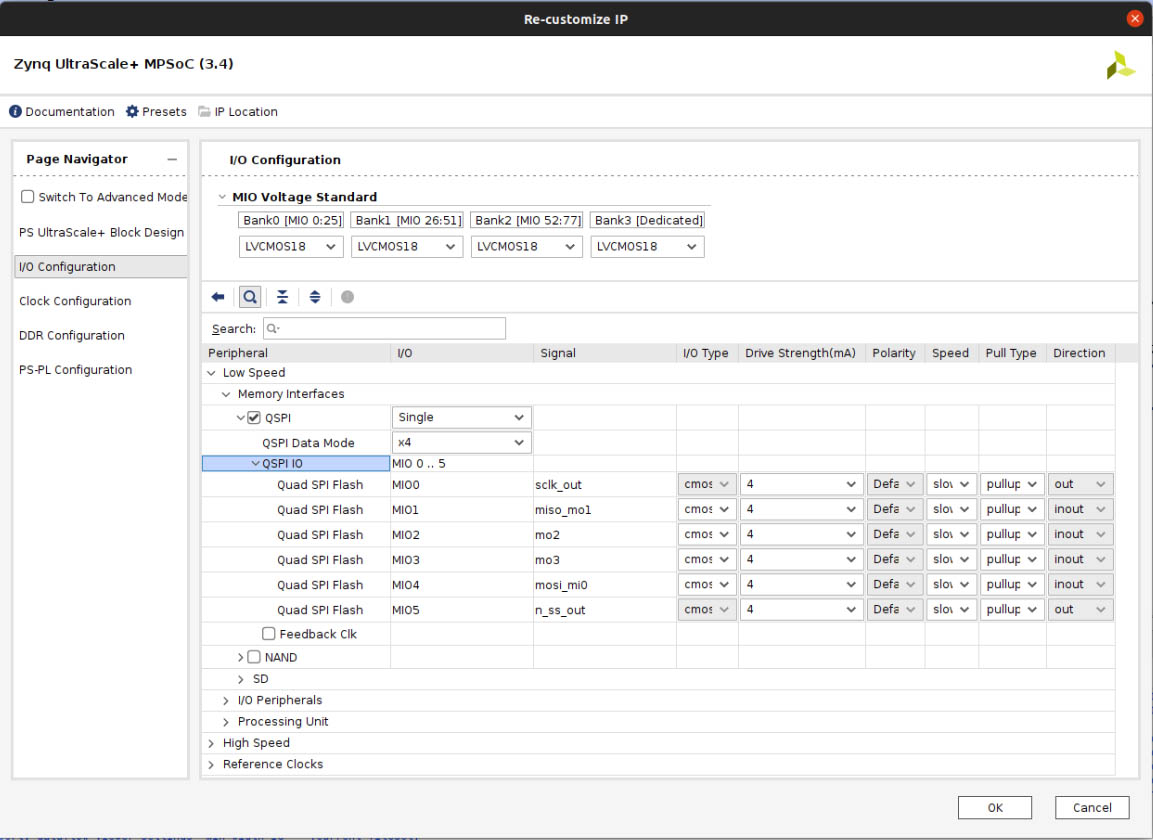
\includegraphics[width=0.95\textwidth]{src/png/kr26-xilinx-vivado-flow/kr26-xilix-vivado-flow-17.jpg}
					\caption{Xilinx Vivado – \gls{abbreviation:ps} \gls{abbreviation:io} Configuration \gls{abbreviation:qspi} zařízení.}
					\label{fig:kr26-xilix-vivado-flow-17}
				\end{figure}

				\begin{figure}[htbp!]
					\centering
					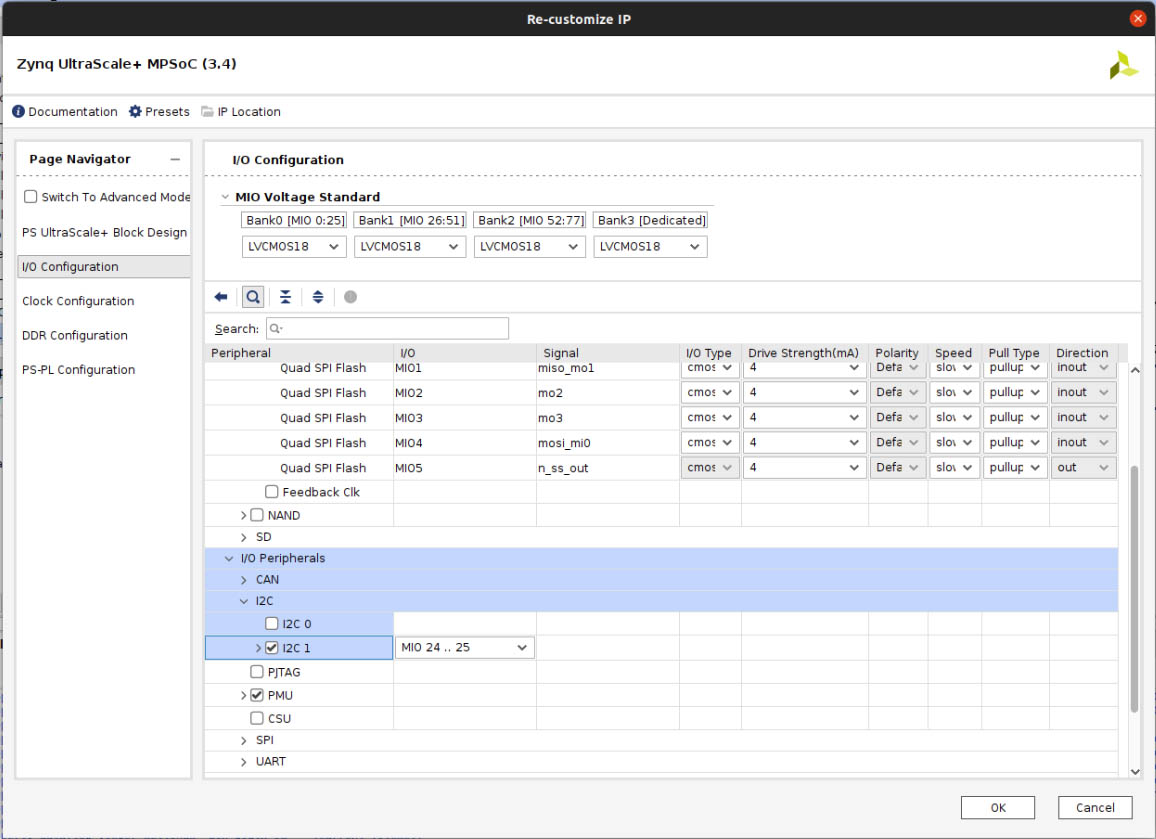
\includegraphics[width=0.95\textwidth]{src/png/kr26-xilinx-vivado-flow/kr26-xilix-vivado-flow-18.jpg}
					\caption{Xilinx Vivado – \gls{abbreviation:ps} \gls{abbreviation:io} Configuration \gls{abbreviation:iic} zařízení.}
					\label{fig:kr26-xilix-vivado-flow-18}
				\end{figure}


				\begin{figure}[htbp!]
					\centering
					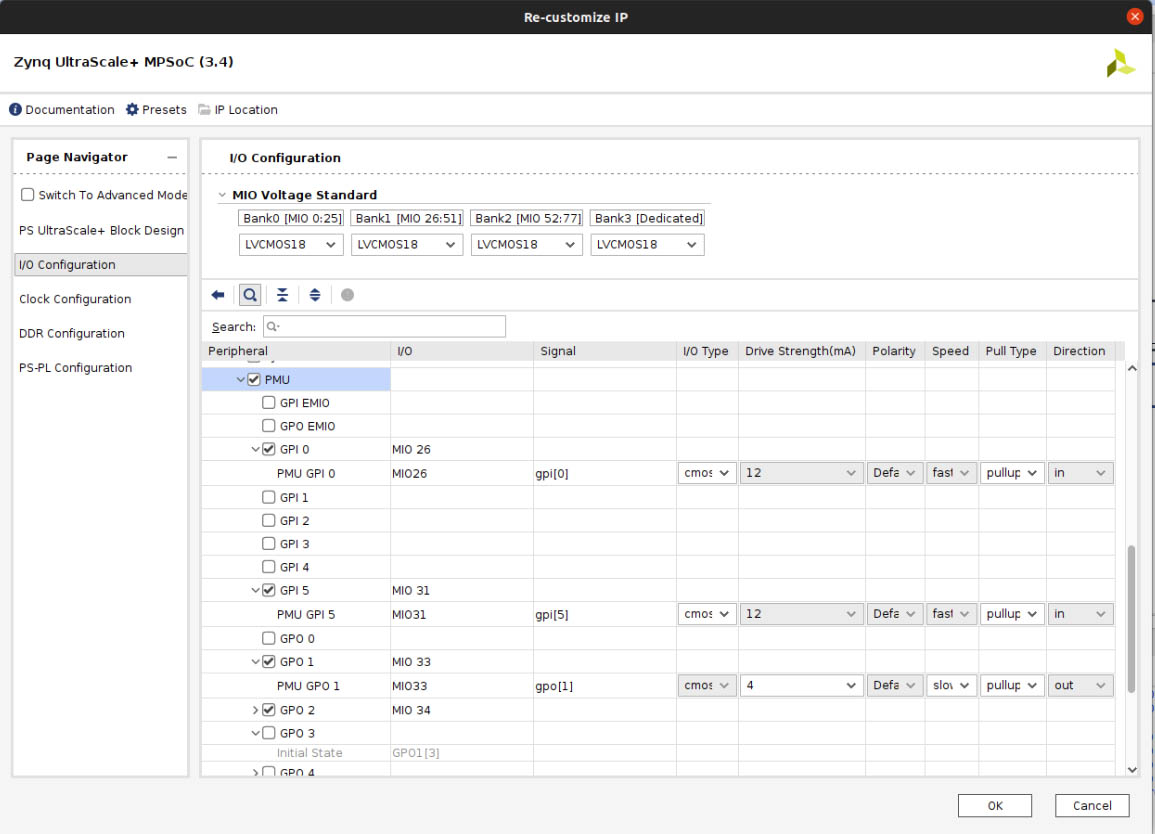
\includegraphics[width=0.95\textwidth]{src/png/kr26-xilinx-vivado-flow/kr26-xilix-vivado-flow-19.jpg}
					\caption{Xilinx Vivado – \gls{abbreviation:ps} \gls{abbreviation:io} Configuration PMU (\gls{abbreviation:gpio} 4 a \gls{abbreviation:gpio} 5 není vybráno).}
					\label{fig:kr26-xilix-vivado-flow-19}
				\end{figure}

				\begin{figure}[htbp!]
					\centering
					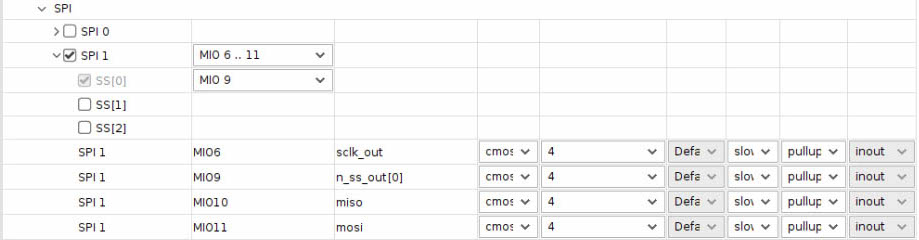
\includegraphics[width=0.95\textwidth]{src/png/kr26-xilinx-vivado-flow/kr26-xilix-vivado-flow-20.jpg}
					\caption{Xilinx Vivado – \gls{abbreviation:ps} \gls{abbreviation:io} Configuration \gls{abbreviation:spi} zařízení.}
					\label{fig:kr26-xilix-vivado-flow-20}
				\end{figure}

				\begin{figure}[htbp!]
					\centering
					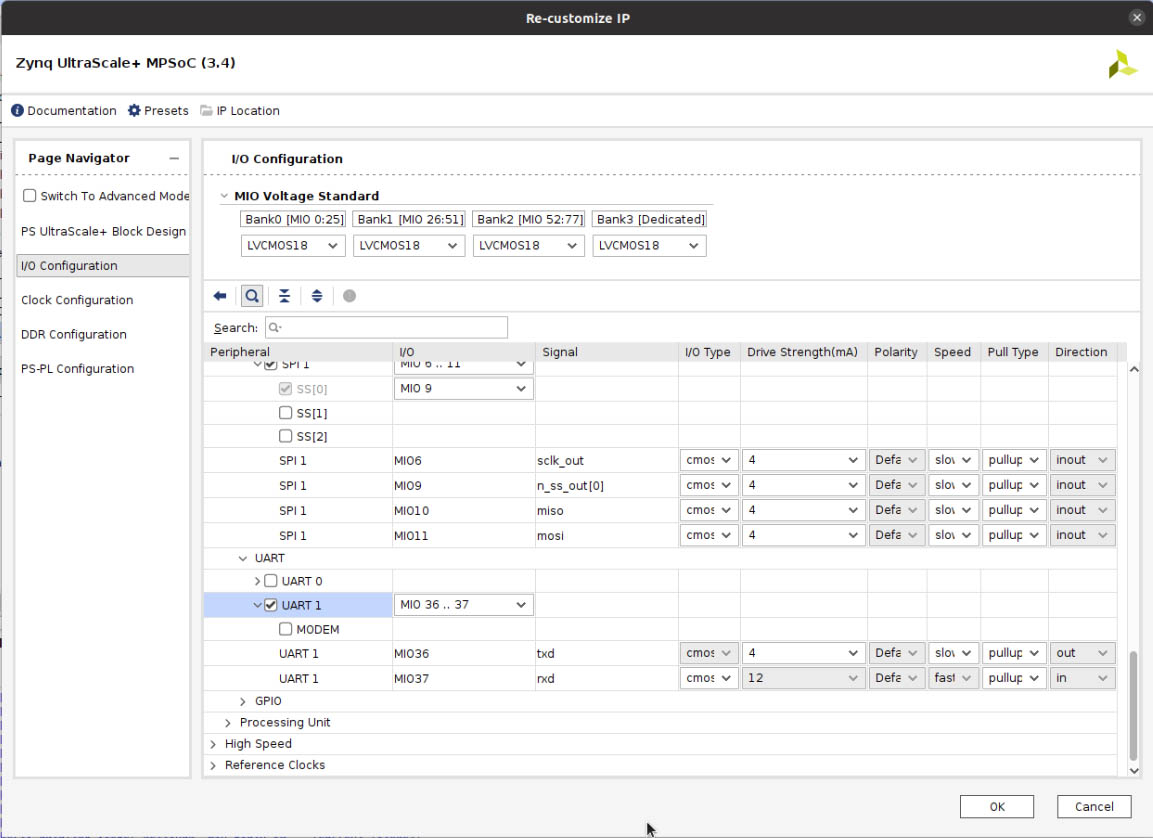
\includegraphics[width=0.95\textwidth]{src/png/kr26-xilinx-vivado-flow/kr26-xilix-vivado-flow-21.jpg}
					\caption{Xilinx Vivado – \gls{abbreviation:ps} \gls{abbreviation:io} Configuration \gls{abbreviation:uart} zařízení.}
					\label{fig:kr26-xilix-vivado-flow-21}
				\end{figure}

				\begin{figure}[htbp!]
					\centering
					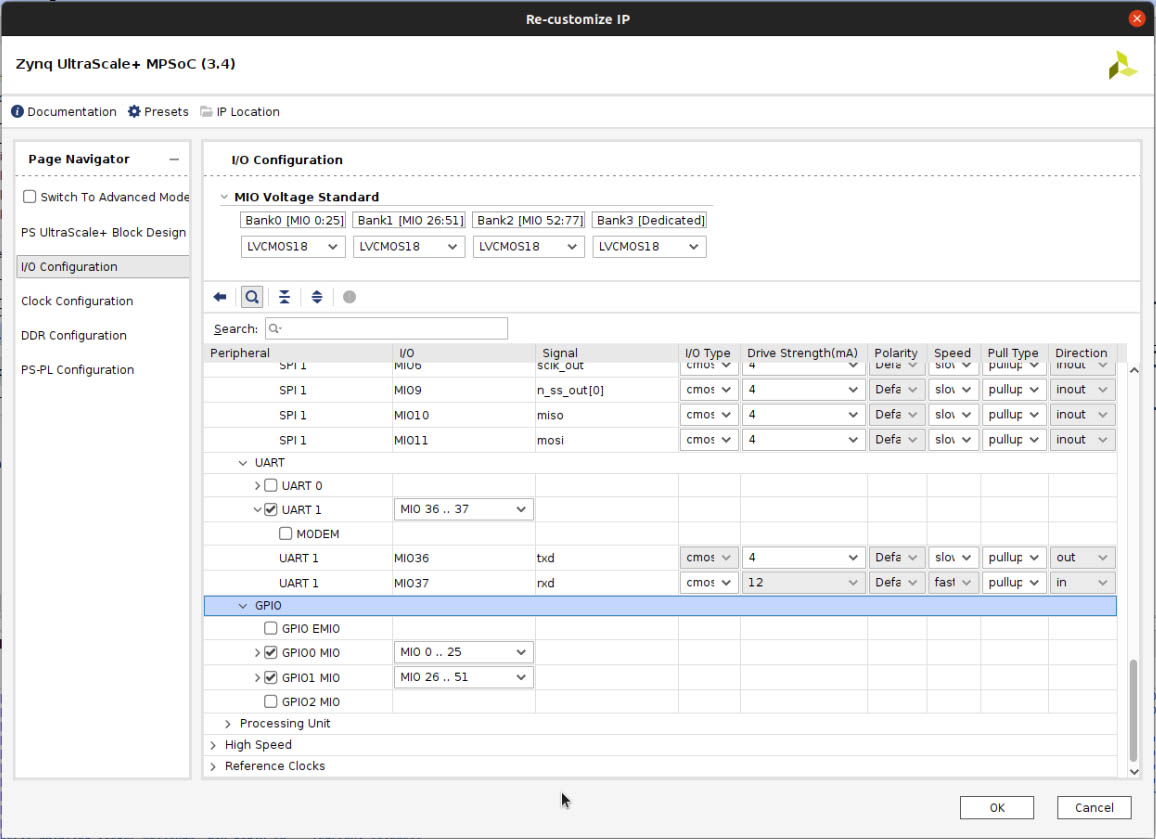
\includegraphics[width=0.95\textwidth]{src/png/kr26-xilinx-vivado-flow/kr26-xilix-vivado-flow-22.jpg}
					\caption{Xilinx Vivado – \gls{abbreviation:ps} \gls{abbreviation:io} Configuration \gls{abbreviation:gpio} zařízení.}
					\label{fig:kr26-xilix-vivado-flow-22}
				\end{figure}


				\begin{figure}[htbp!]
					\centering
					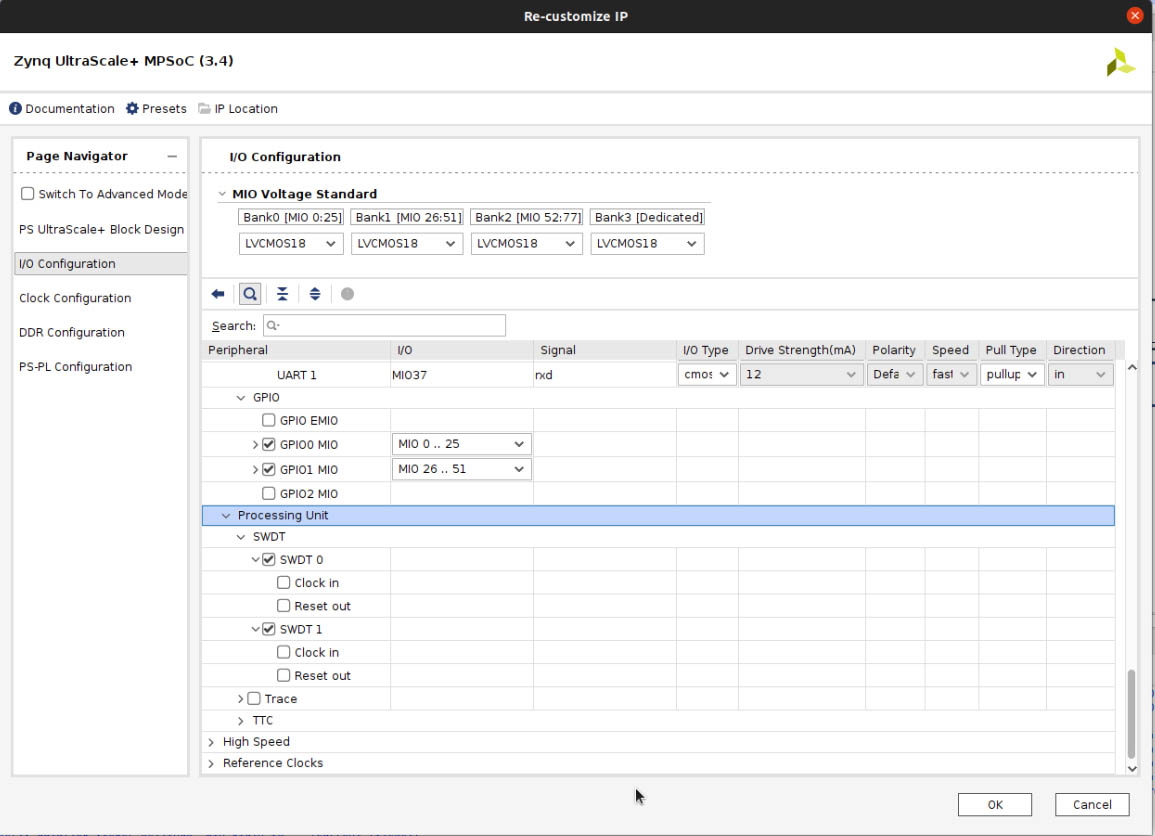
\includegraphics[width=0.95\textwidth]{src/png/kr26-xilinx-vivado-flow/kr26-xilix-vivado-flow-23.jpg}
					\caption{Xilinx Vivado – \gls{abbreviation:ps} \gls{abbreviation:io} Configuration System Watchdog Timers (SWDT).}
					\label{fig:kr26-xilix-vivado-flow-23}
				\end{figure}

				\begin{figure}[htbp!]
					\centering
					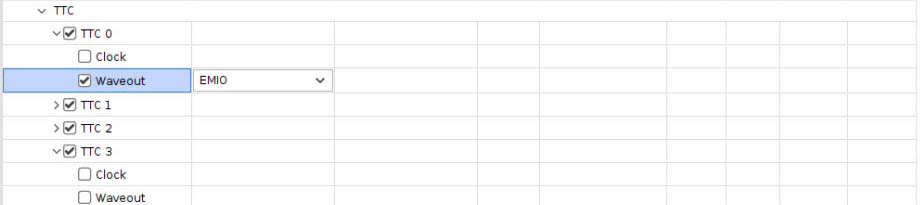
\includegraphics[width=0.95\textwidth]{src/png/kr26-xilinx-vivado-flow/kr26-xilix-vivado-flow-30.jpg}
					\caption{Xilinx Vivado – \gls{abbreviation:ps} \gls{abbreviation:io} Configuration Triple Timer Counter (TTC), TTC 0 výstup Waveout je využit pro PIN řídící chladící ventilátor na \gls{abbreviation:som}.}
					\label{fig:kr26-xilix-vivado-flow-30}
				\end{figure}

				\begin{figure}[htbp!]
					\centering
					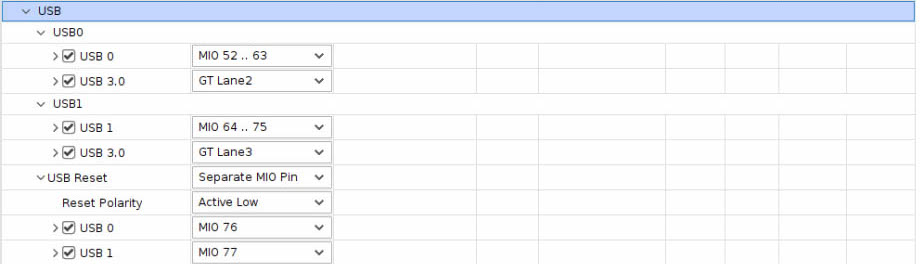
\includegraphics[width=0.95\textwidth]{src/png/kr26-xilinx-vivado-flow/kr26-xilix-vivado-flow-25.jpg}
					\caption{Xilinx Vivado – \gls{abbreviation:ps} \gls{abbreviation:io} Configuration \gls{abbreviation:usb}.}
					\label{fig:kr26-xilix-vivado-flow-25}
				\end{figure}

				\begin{figure}[htbp!]
					\centering
					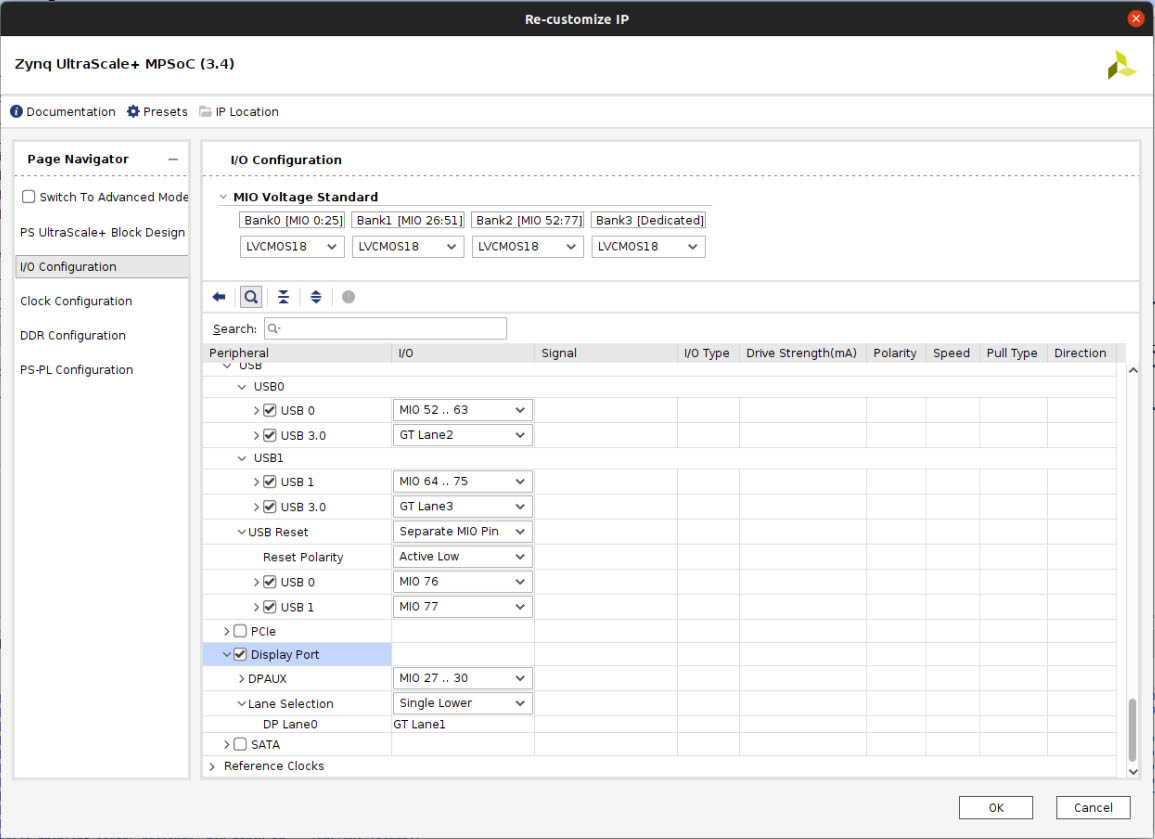
\includegraphics[width=0.95\textwidth]{src/png/kr26-xilinx-vivado-flow/kr26-xilix-vivado-flow-26.jpg}
					\caption{Xilinx Vivado – \gls{abbreviation:ps} \gls{abbreviation:io} Configuration DisplayPort.}
					\label{fig:kr26-xilix-vivado-flow-26}
				\end{figure}

				\fbar
				Po úspěšné konfiguraci \gls{abbreviation:io} je možné přistoupit ke kartě \textit{\gls{abbreviation:ps}-\gls{abbreviation:pl} Configuration} a v~záložce \textit{General -> Fabric Reset Enable} povolit \textit{Fabric Reset Enable} a zvolit v~nabídce \textit{Number of Fabric Resets} číslo 4.\par
				Nastavení \textit{Number of Fabric Resets} udává, kolik signálů je možné použít pro reset \gls{abbreviation:ip} bloků realizovaných v~\gls{abbreviation:pl}. \cite{xilinx-ultra-scale-plus-mpsoc-processing-syste-product-guide} \cite{xilinx-wiki-atlassian-zynq-ultra-scale-plus-mpsoc-restart-solution}\par

				V~předchozích krocích byla představena základní konfigurace \gls{abbreviation:ps} pro funkčnost periferií, přítomných na vývojové desce Xilinx Kria KR260 s~\texttt{Zynq UltraScale+ MPSoC}. Po provedení konfigurace je možné v~konfigurační nabídce \gls{abbreviation:ps} \gls{abbreviation:ip} v~kartě \textit{\gls{abbreviation:ps} UltraScale+ Block Design} pozorovat u~konfigurovaných prvků označení pomocí „$\checkmark$“ symbolu. Ukázka systému je zobrazena na obr. \ref{fig:kr26-xilix-vivado-flow-28}.

				\begin{figure}[htbp!]
					\centering
					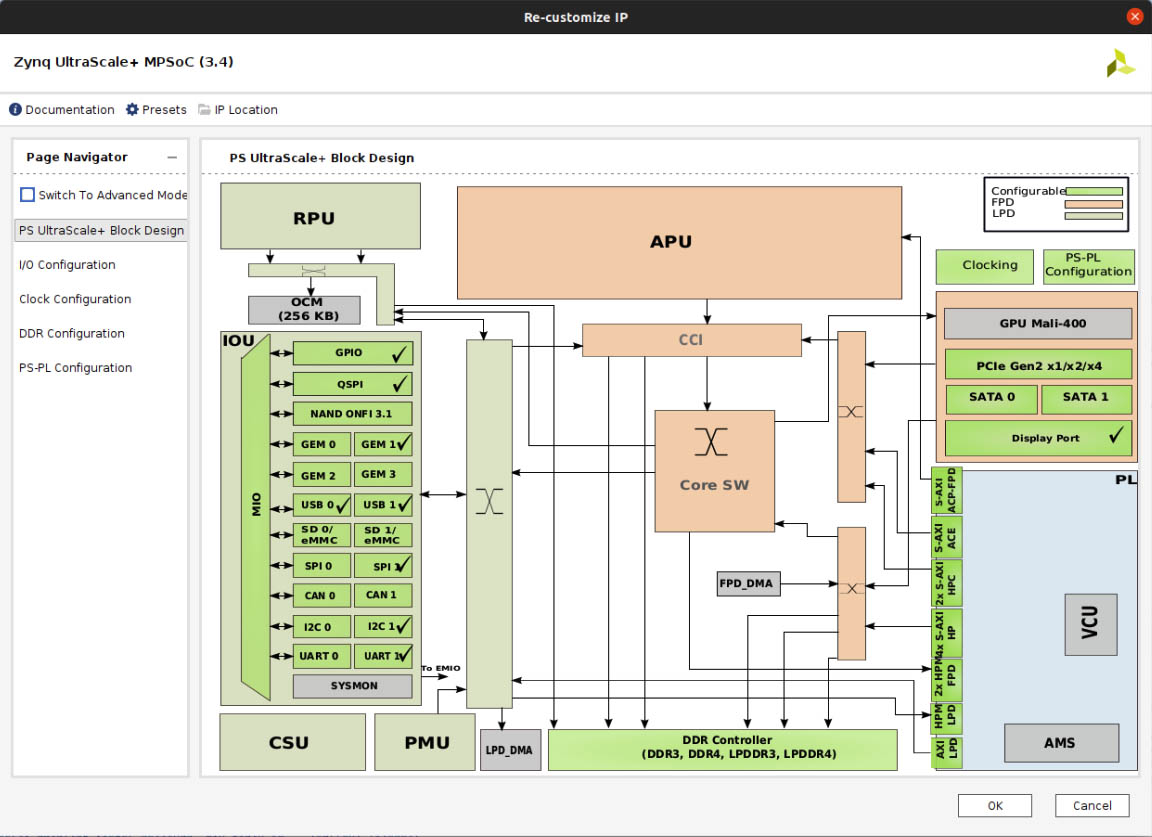
\includegraphics[width=0.85\textwidth]{src/png/kr26-xilinx-vivado-flow/kr26-xilix-vivado-flow-28.jpg}
					\caption{Xilinx Vivado – \gls{abbreviation:ps} UltraScale+ Block Design v~\gls{abbreviation:ps} \gls{abbreviation:ip}.}
					\label{fig:kr26-xilix-vivado-flow-28}
				\end{figure}

			\subsubsection{Design Constraints}
				Aby bylo možné vytvořené \textit{virtuální} piny ve Vivado propojit se skutečnými fyzickými piny \gls{abbreviation:mpsoc}, resp. fyzickými piny vývojové desky, je třeba vytvořit soubor v~prostředí Vivado, který toto fyzické propojení definuje. Tyto soubory se nazývají \textit{Constraints Files}.\par
				Jejich tvorba může probíhat i mimo prostředí Vivado, jsou to textové soubory, jež lze upravit v~libovolném textovém editoru. Tato skutečnost lze využít při časté tvorbě designů v~nových projektech pro zrychlení konfigurace. Soubory je poté možné jednoduše importovat.\par
				Soubory se vkládají pomocí výběru v~levém menu \textit{Project Manager -> Add Sources -> Add or create constraints -> Add Files/Create File}. Nabídka tvorby souboru je vyzobrazena na obr. \ref{fig:kr26-xilix-vivado-flow-32}.\par

				\begin{figure}[htbp!]
					\centering
					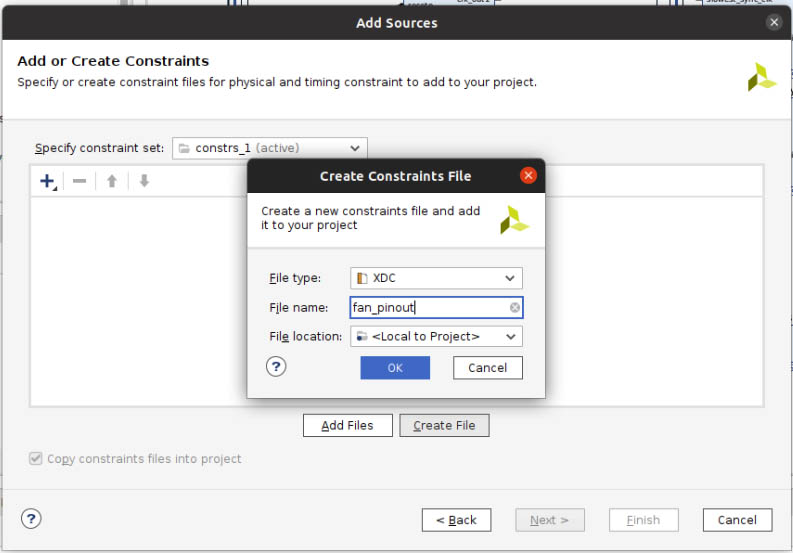
\includegraphics[width=0.85\textwidth]{src/png/kr26-xilinx-vivado-flow/kr26-xilix-vivado-flow-32.jpg}
					\caption{Xilinx Vivado – okno tvorby/vložení Constraints File.}
					\label{fig:kr26-xilix-vivado-flow-32}
				\end{figure}

				Pro spojení vytvořeného virtuálního pinu \texttt{fan\_en\_b} a fyzického pinu, ke kterému je na \gls{abbreviation:cc} připojen ventilátor, je do \texttt{\gls{abbreviation:xdc}} souboru zapsána konfigurace z~kódu \ref{lst:fan-pinout-constraints-file}.\par
				Kód \ref{lst:fan-pinout-constraints-file} byl získán z~\cite{hackster-add-peripherial-support-to-kria-kr260-vivado}. Autorem však bylo ověřeno, že se skutečně jedná o~fyzický pin \texttt{A12}.\par
				
				


				\begin{lstlisting}[language={xdc}, caption={Constraints \gls{abbreviation:xdc} soubor pro přiřazení \gls{abbreviation:pl} Vivado pinu fan\_en\_b k~fyzickému pinu \gls{abbreviation:mpsoc} na \gls{abbreviation:cc}.}, label= {lst:fan-pinout-constraints-file}]
set_property BITSTREAM.GENERAL.COMPRESS TRUE [current_design]
					
# Fan Speed Enable
set_property PACKAGE_PIN A12 [get_ports {fan_en_b}]
set_property IOSTANDARD LVCMOS33 [get_ports {fan_en_b}]
set_property SLEW SLOW [get_ports {fan_en_b}]
set_property DRIVE 4 [get_ports {fan_en_b}]\end{lstlisting}

				Vyhledání propojení fyzického pinu a označení pro soubory \texttt{\gls{abbreviation:xdc}} probíhá totožně pro konektory \textit{\gls{abbreviation:pmod}} a \textit{Raspberry Pi HAT}. Oficiální dokumentace pro postup vyhledání pinů nebyla autorem nalezena, proto se pokusil nalézt vlastní postup, který ověřil na oficiálním fóru Xilinx \cite{xilinx-support-forum-petrzakopal-schematic-vs-constrains-pin-confusion-explanation}.\par
				\vspace*{0.55cm}
				Postup nalezení reálného pinu je následující:
				\begin{enumerate}
					\item Nalézt ve schématu \cite{kria-kr260-starter-kit-cc-schematics} Kria KR260 \gls{abbreviation:cc} požadované označení fyzického pinu (např. pro ventilátor \texttt{HDA20}).
					\item Nalézt ve schématu \cite{kria-kr260-starter-kit-cc-schematics}, ke kterému pinu na \gls{abbreviation:pl} konektoru (\texttt{SOM240\_1 CONNECTOR}) je nalezený PIN připojen. (v~případě ventilátoru \texttt{C24}).
					\item V~\gls{abbreviation:xdc} \cite{kria-k26-som-xdc} souboru pro Xilinx Kria K26 vyhledat udaný pin v~připojení konektoru a zkontrolovat, zda je připojen ke správnému konektoru ze schématu a získat požadované označení \texttt{PACKAGE\_PIN}.
				\end{enumerate}
				\vspace*{0.75cm}
				\fbar
				Po provedení všech pořebných nastavení a konfigurací je možné přejít k~finální části postupu ve Vivado.\par
				Nejprve je vhodné vytvořený design validovat pomocí symbolu „$\checkmark$“ v~ovládací liště v~okně \textit{Platform}. Pokud jsou získány upozornění s~označením \textit{Warning}, je možné pokračovat v~tvorbě platformy. V~bloku \textit{Sources} zvolit pravým tlačítkem vytvořený block design a aktivovat nabídku \textit{Generate Output Products}. Objeví se konfigurační okno, ve kterém je vhodné nastavit v~části \textit{Synthesis Options} volbu \textit{Out of context per \gls{abbreviation:ip}}. V~části \textit{Run Settings} je možné zvolit kolik jader procesoru se bude podílet na zvolené činnosti. Pro osobní počítače autor doporučuje zvolit méně než polovinu dostupných jader \gls{abbreviation:cpu}. Bylo vypozorováno, že pokud jader je zvoleno více, může zatížení systému způsobit samovolné ukončení programmu Vivado.\par
				Po ukončení generace je možné zvolit v~nabídce pro block design akci \textit{Create \gls{abbreviation:hdl} Wrapper}. V~nabídce akce je výhodné využít možnost \textit{Let Vivado manage wrapper and auto update}, kdy Vivado bude aktualizovat \gls{abbreviation:hdl} wrapper podle změn provedených v~designu.\par
				Autorovi se ovšem při změně block designu vyplatilo \gls{abbreviation:hdl} Wrapper kompletně smazat a opětovaně provést kroky \textit{Generate Output Products} a \textit{Create \gls{abbreviation:hdl} Wrapper}.\par
				Nyní je již možné přistoupit k~syntéze, implementaci a generování bit streamu. Jednotlivé kroky je možné pomocí levé nabídky ve Vivado aktivovat samostatně, nebo zvolit pouze generování bit streamu a Vivado automaticky zajistí, že pokud došlo ke změně designu, budou provedeny kroky syntézy a implementace automaticky.\par
				Po úspěšném provedení generování bitstreamu je možné platformu exportovat pro její další využití v~\textit{PetaLinux Tools} a Vitis. Export je možné provést pomocí volby \textit{File -> Export -> Export Platform}. Ve zobrazené nabídce je obecně u~vývojových desek vhodné zvolit \textit{Hardware and hardware emulation}. Dle~\cite{hackster-add-peripherial-support-to-kria-kr260-vivado} podpora \gls{abbreviation:hw} emulace pro K26 není aktuálně dostupná. Posledním krokem je v~nastavení \textit{Platform State} vybrání volby \textit{Pre-synthesis} a \textit{Include bitstream}. Po označení platformy je možné provést export.\par
				V~této části byl představen postup tvorby základní \gls{abbreviation:hw} platfromy pro Xilinx KR260 Starter Kit vývojovou desku v~prostředí Vivado. Výstupem projektu ve Vivado je soubor \textit{\gls{abbreviation:xpr}}, který je dále využit při tvorbě akcelerované aplikace v~\textit{PetaLinux Tools} a Vitis. Pro některé případy, kdy není potřeba specifický \gls{abbreviation:hw} v~\gls{abbreviation:pl} je možné využít předpřipravené \textit{\gls{abbreviation:xpr}} soubory. Tyto předpřipravené soubory slouží pouze k~seznámení s~vývojovými deskami a nejsou dostačující pro vývoj specifické akcelerované aplikace.
				
			\fbar
			\subsubsection{HW block design vyvíjené aplikace}\label{subsubsec:hw-block-design-vyvijene-aplikace}
				Představený design na obr. \ref{fig:kr-26-xilinx-vivado-hw-block-design} je využit pro tvorbu platformy pro akcelerované aplikace v~této práci. Platforma využívá \gls{abbreviation:spi} komunikaci, realizovanou v~\gls{abbreviation:pl} a blok \gls{abbreviation:axi} Timer.\par
			\begin{figure}[htbp!]
				\centering
				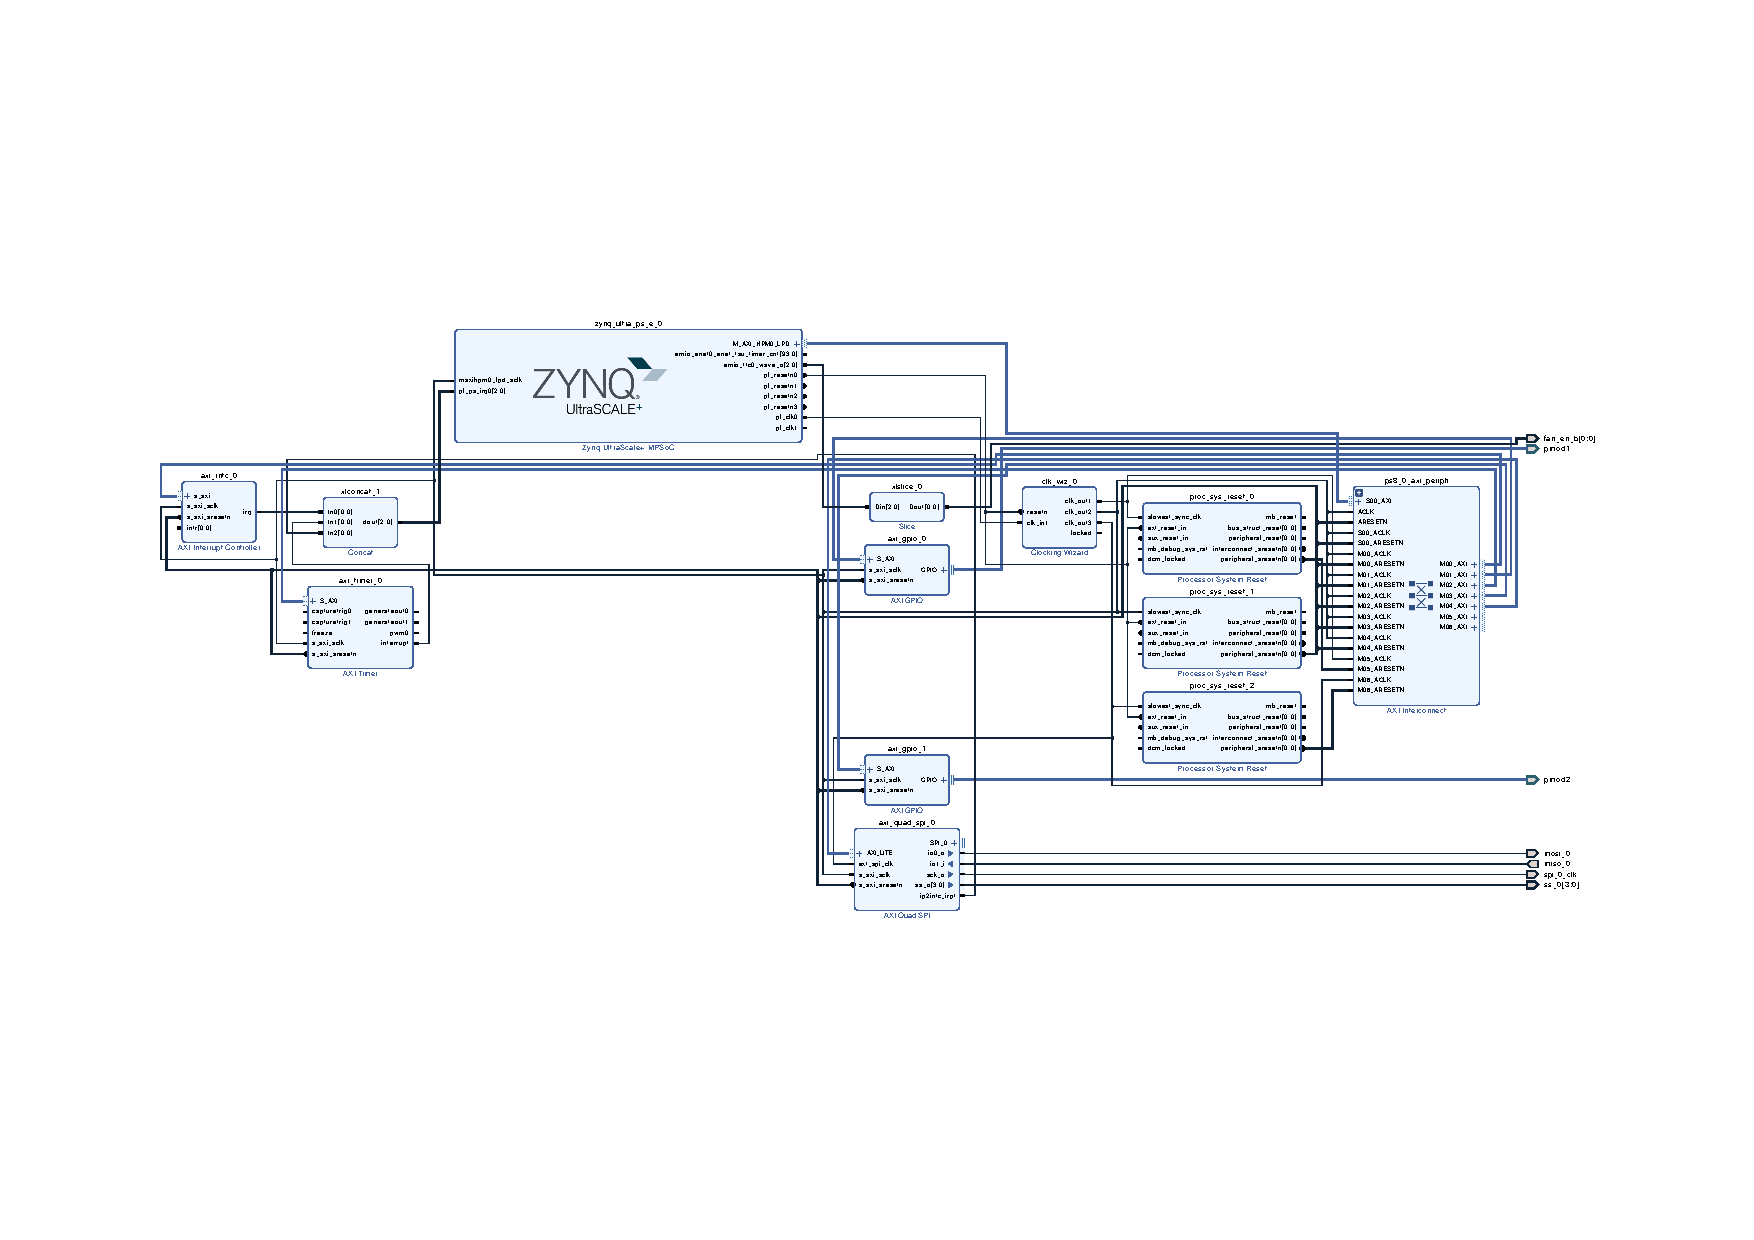
\includegraphics[width=0.78\paperheight, angle=90, origin=c]{src/pdf/kr-26-xilinx-vivado-hw-block-design.pdf}
				\caption{Xilinx Vivado – \gls{abbreviation:hw} block design vyvíjené aplikace.}
				\label{fig:kr-26-xilinx-vivado-hw-block-design}
			\end{figure}


	\fbar
	\section{Tvorba PetaLinux}\label{subsec:tvorba-petalinux}
	Jak již bylo zmíněno v~části \hyperref[subsec:aplikace-a-operacni-system]{\textit{Aplikace a operační systém}}, aplikace pro Xilinx Kria je možné vytvářen pro \textit{Bare Metal / Standalone}, \textit{PetaLinux} a také distribuci operačního systému Linux \textit{Ubuntu}. V~této práci je využito systému \textit{PetaLinux}, který díky své tvorbě pomocí \textit{PetaLinux Tools} je možné konfigurovat tak, aby využíval \gls{abbreviation:hw} konfigurovaný v~\gls{abbreviation:pl} a splňoval požadavky vytvářené aplikace.\par
	Konfigurace pro jednotlivé požadavky vytvářených aplikací se mohou odlišovat, ovšem rámec (flow) tvorby systému zůstává pro danou platformu zachován. V~této práci bude představen postup tvorby \textit{PetaLinux} systému pro \gls{abbreviation:hw} platformu obsahující prvky, představené v~části \hyperref[subsubsec:hw-block-design-vyvijene-aplikace]{\textit{HW block design vyvíjené aplikace}}.\par
	Postup tvorby \textit{PetaLinux} systému čerpá informace z~\cite{hackster-getting-started-with-the-kria-kr260-in-petalinux}, \cite{xilinx-github-vitis-tutorials-step-2-create-the-software-components} a z~experimentálních zjištění autora práce.\par
	Prvním krokem je aktivace \textit{PetaLinux} prostředí (environment). Příkaz k~aktivaci je závislý na umístění instalovaných \textit{PetaLinux Tools} a je zobrazen v~kódu \ref{lst:petalinux-environment}. Představený postup předpokládá práci s~definovanou strukturou projektu, definovanou v~části \hyperref[sec:struktura-slozek]{\textit{Struktura složek}} v~kódu \ref{lst:struktura-slozek}.


	\begin{lstlisting}[language={sh}, caption={Aktivace prostředí PetaLinux verze 2022.2.}, label= {lst:petalinux-environment}, morekeywords={source}]
source /tools/Xilinx/PetaLinux/2022.2/settings.sh\end{lstlisting}

	Po aktivaci prostředí je možné vytvořit projekt pomocí příkazu \ref{lst:petalinux-create}. Soubor \texttt{xilinx-kr260-starterkit-v2022.2-10141622.bsp} (\gls{abbreviation:bsp}) je pro aktuální využívanou verzi vývojových nástrojů možné stáhnout z~oficiálních stránek Xilinx \cite{xilinx-downloads}.

	\begin{lstlisting}[language={sh}, caption={Tvorba PetaLinux projektu ze základního \gls{abbreviation:bsp} souboru.}, label= {lst:petalinux-create}, morekeywords={petalinux-build, petalinux-package, petalinux-config, petalinux-create}]
# general command
petalinux-create --type project -s <path-to-bsp-file> --name <project-name>

# example command for defined file structure
petalinux-create --type project -s ./../xilinx-kr260-starterkit-v2022.2-10141622.bsp --name petalinux\end{lstlisting}

	\fbar
	\subsection{Hardware konfigurace PetaLinux}
	Nyní je možné přejít do adresáře projektu pomocí \texttt{cd <project-name>} a začít konfigurovat \textit{PetaLinux}.\par
	První konfigurace spočívá v~načtení \gls{abbreviation:hw} platformy do projektu pomocí příkazu \ref{lst:petalinux-config-hw}. Kdy je předpokládáno, že ve složce \texttt{hw} je umístěn soubor exportované platformy z~Vivado, získaný v~části \hyperref[subsec:tvorba-hw-designu-pro-xilinx-kria-kr260]{\textit{Tvorba HW designu pro Xilinx Kria KR260 vývojovou desku}}.\par


	\begin{lstlisting}[language={sh}, caption={Konfigurace PetaLinux pomocí \gls{abbreviation:xpr} souboru z~Vivado.}, label= {lst:petalinux-config-hw}, morekeywords={petalinux-build, petalinux-package, petalinux-config}]
petalinux-config --get-hw-description=./../hw/\end{lstlisting}

	Po načtení \textit{\gls{abbreviation:xsa}} souboru je v~terminálu zobrazena konfigurační nabídka. Nastavení prvků v~této nabídce je pro K26 \gls{abbreviation:som} uvedeno v~kódu \ref{lst:petalinux-config-hw-settings}.



\begin{lstlisting}[language={sh}, caption={Nastavení v~petalinux-config pro Xilix K26 SOM.}, label= {lst:petalinux-config-hw-settings}]
FPGA Manager -> Fpga Manager <*>

Image Packaging Configuration -> Root Filesystem Type --> INITRD <*>
Image Packaging Configuration -> INITRAMFS/INITRD Image name -> petalinux-initramfs-image <*>
Image Packaging Configuration -> Copy final images to tftpboot < >\end{lstlisting}

	Pátý řádek popisuje vypnutí možnosti kopírování souborů pomocí \texttt{tftpboot}. Tato možnost nebyla v~této práci využita a prozkoumána.\par
	Ukázka konfigurační nabídky, která je zobrazena uživateli je na obr. \ref{fig:terminal-petalinux-config}.\par

\begin{figure}[htbp!]
	\centering
	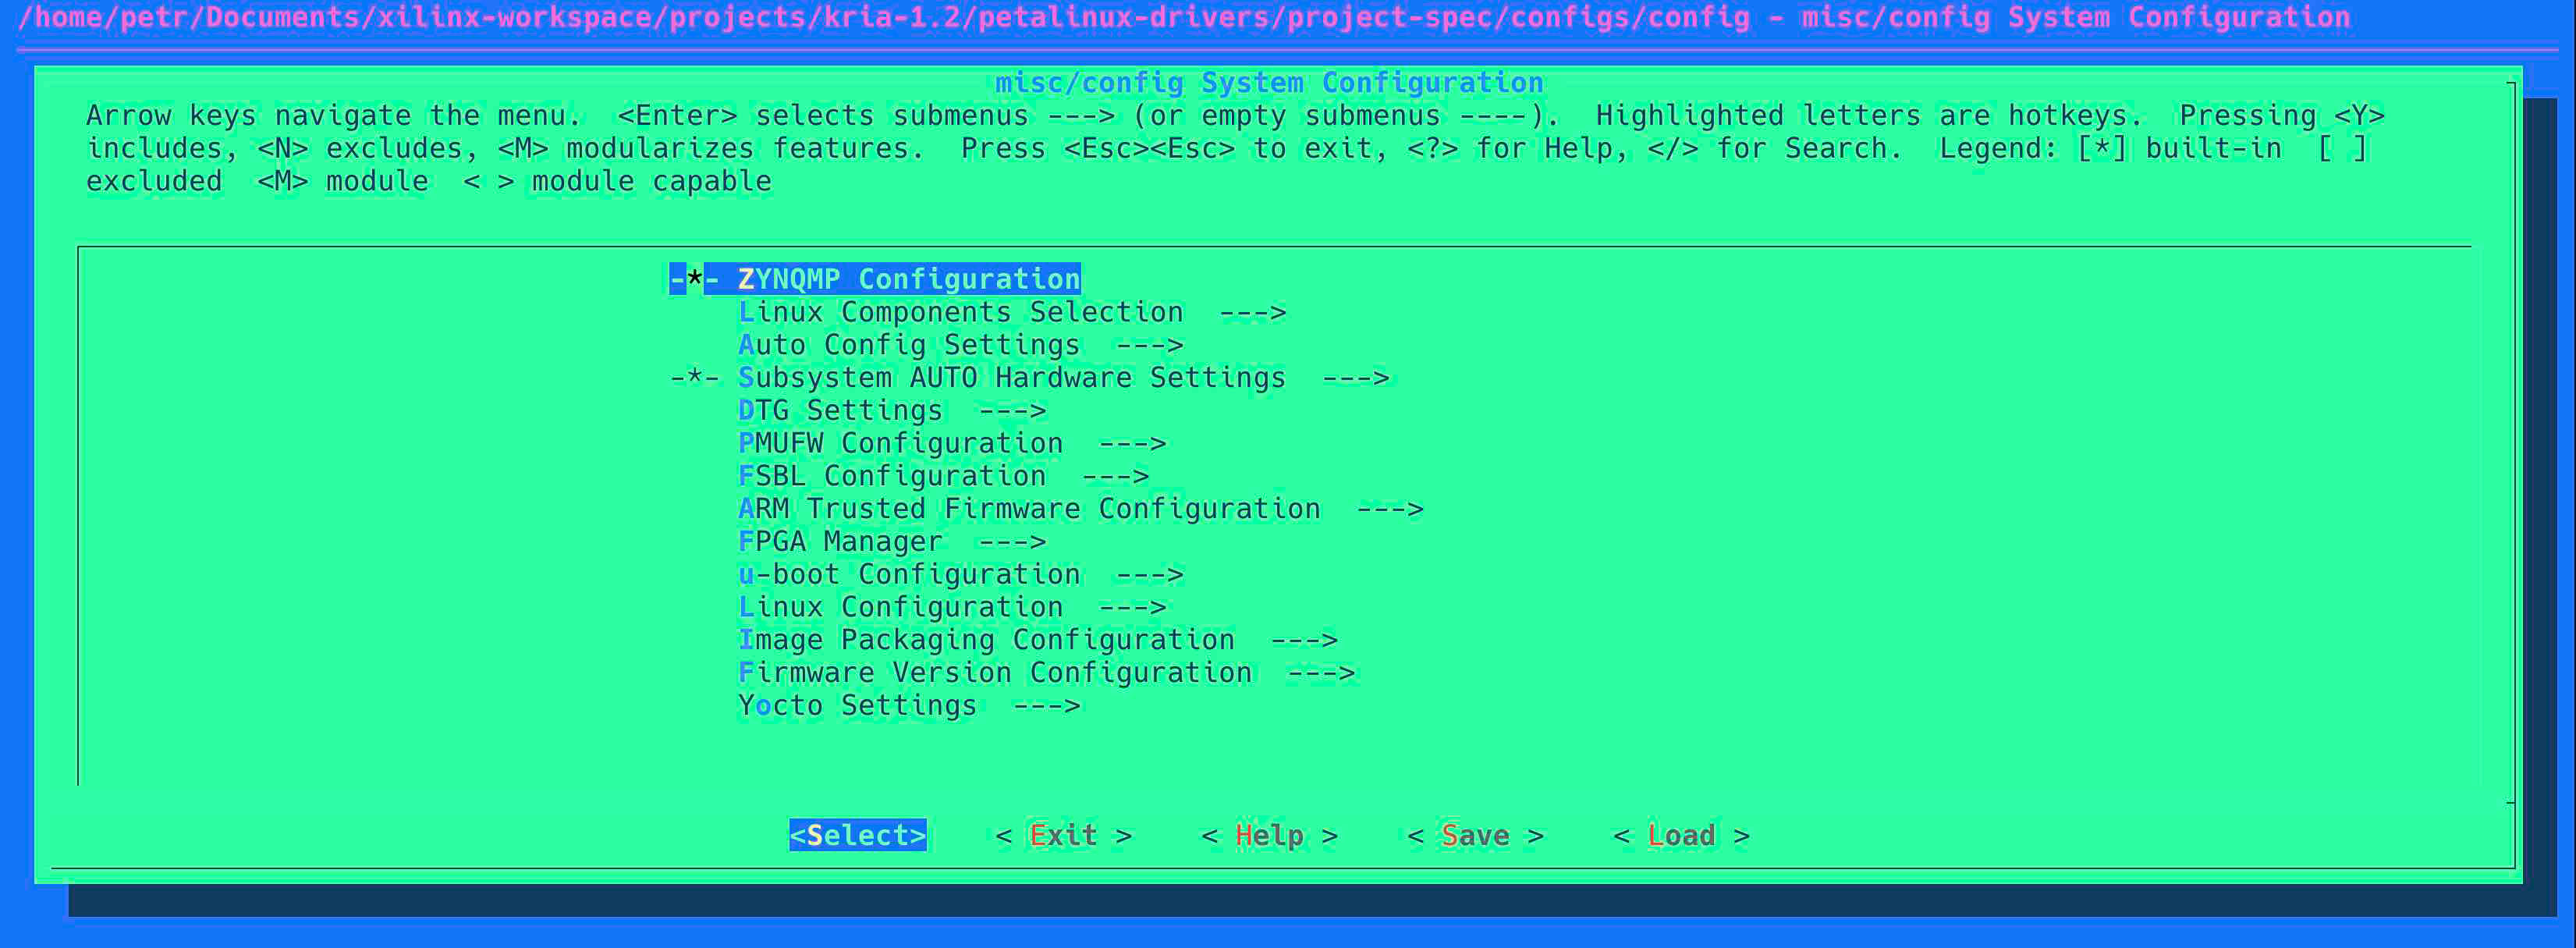
\includegraphics[width=1\textwidth]{src/jpg/terminal-petalinux-config-crop.jpg}
	\caption{Xilinx Vivado – snímek obrazovky konfigurace PetaLinux pomocí „petalinux-config“ příkazu.}
	\label{fig:terminal-petalinux-config}
\end{figure}


	Bylo zjištěno, že při tvorbě systému s~aplikovaným \gls{abbreviation:rt} patchem pro \textit{PetaLinux} je vhodné provést úvodní build systému bez dodatečných konfigurací a poté build opakovat s~požadovanými konfiguracemi. Build proces je spuštěn příkazem \ref{lst:petalinux-build}.\par
	Proces aplikace \gls{abbreviation:rt} patche je představen v~části \hyperref[subsubsec:postup-aplikace-preempt-rt-patch]{\textit{Postup aplikace PREEMPT\_\gls{abbreviation:rt} patch}}.\par

\begin{lstlisting}[language={sh}, caption={PetaLinux build příkaz pro vytvoření systému.}, label= {lst:petalinux-build}, morekeywords={petalinux-build, petalinux-package, petalinux-config}]
petalinux-build\end{lstlisting}

	\subsection{Konfigurace jádra PetaLinux}
	Po aplikaci patche je vhodné pokračovat nastavením jádra (pro jádro systému je zavedeno také označení kernel) \textit{PetaLinux} systému pomocí příkazu \ref{lst:petalinux-config-c-kernel}. Ve vytvářené aplikaci je využíván \texttt{Userspace IO Driver} a proto je nutné aktivovat konfiguraci jádra, která zajistí automatické načtení driveru (ovladače) do systému při jeho startu. Pokud by se tak nestalo, bylo by nutné vkládat moduly manuálně pomocí příkazů \texttt{modprobe} či \texttt{insmod}. Při konfiguraci jádra je možné aktivovat i další prvky, které nejsou v~této práci využívány. Ukázka konfigurace pro \texttt{Userspace IO Driver} je zobrazena v~kódu~\ref{lst:petalinux-config-c-kernel-userspace-io-driver}.\par

\begin{lstlisting}[language={sh}, caption={PetaLinux příkaz pro konfiguraci jádra systému.}, label= {lst:petalinux-config-c-kernel}, morekeywords={petalinux-build, petalinux-package, petalinux-config}]
petalinux-config -c kernel\end{lstlisting}

\begin{lstlisting}[language={sh}, caption={PetaLinux konfigurace pro User Space IO Driver.}, label= {lst:petalinux-config-c-kernel-userspace-io-driver}]
Device drivers -> user space IO drivers <\*>
Device drivers -> user space IO drivers -> Userspace platform driver with generic irq and dynamic memory <*>
Device drivers -> user space IO drivers -> Userspace platform driver with generic IRQ handling <*>\end{lstlisting}

		\fbar
		\subsubsection{Konfigurace Device Tree}\label{subsubsec:konfigurace-device-tree}
		Aby bylo možné využívat zmiňovaný \texttt{Userspace IO Driver} v~podobě \texttt{generic-uio} driveru pro řešení přerušení (interrupts) od prvků \gls{abbreviation:axi} Quad \gls{abbreviation:spi} \cite{axi-quad-spi-ip-product-guide}, \gls{abbreviation:axi} Timer \cite{axi-timer-v-2-0-ip-product-guide} a dalších, je nezbytné provést odpovídající konfiguraci \texttt{devicetree}. Konfiguraci \texttt{devicetree} je možné provádět i u~tvorby Linux systému pro jiné vývojové desky s~\gls{abbreviation:soc}, které neobsahují \gls{abbreviation:fpga}, ale využívají systému Linux.\par
		Problematika \texttt{devicetree} je značně obsáhlá, tento standard je obhospodařován komunitou systému Linux a pravidelně jsou vydávány specifikace, které tuto datovou strukturu popisují. Tyto specifikace je možné nalézt na oficiálních stránkách této komunity. \cite{devicetree-org-specification}\par
		Existuje i záznam velmi přínosné prezentace z~\textit{Embedded Linux Conference Europe} ohledně problematiky Device Tree od \textit{Thomas Petazzoni} s~názvem \textit{Device Tree for Dummies!} \cite{youtube-devicetree-for-dummies}.\par
		Při tvorbě akcelerované aplikace v~této práci byl využit \gls{abbreviation:dt} soubor automaticky vytvořený při konfiguraci jádra systému při prvním build procesu \textit{PetaLinux} systému. Ovšem aby bylo možné použít zmiňované bloky, je třeba do souboru \texttt{system-user.dtsi} zapsat požadované konfigurace. Soubor \texttt{system-user.dtsi} překonfiguruje automaticky vytvořený soubor \texttt{system-conf.dtsi}. V~hierarchii načítání konfiguračních souborů je čten \texttt{system-conf.dtsi} jako poslední.\par
		Upravený obsah \texttt{system-user.dtsi} souboru je zobrazen v~\ref{lst:system-user-dtsi-device-tree}. Soubor je možné nalézt v~cestě \texttt{<petalinux-project>/project-spec/meta-user/recipes-bsp/device-tree/\\files/system.user.dtsi}.\par

		\begin{lstlisting}[language={devicetree}, caption={Obsah souboru system-user.dtsi, překonfigurovávající soubor system-conf.dtsi.}, label= {lst:system-user-dtsi-device-tree}]
/include/ "system-conf.dtsi"
/ {
        chosen {
        bootargs = "earlycon clk_ignore_unused   uio_pdrv_genirq.of_id=generic-uio";
        stdout-path = "serial0:115200n8";
        };

    timer@0080020000 {
        compatible = "axi_timer_0, generic-uio, ui_pdrv";
        status = "okay";
        };

    axi_quad_spi@80040000 {
    compatible = "axi_quad_spi_0, generic-uio, ui_pdrv";
    status = "okay";
    };
};\end{lstlisting}

			Tento rekonfigurační \gls{abbreviation:dt} byl získán reengineeringem souboru \texttt{pl.dtsi}. Soubor \texttt{pl.dtsi} je získán za pomoci exportovaného \textit{\gls{abbreviation:xpr}} souboru pomocí \texttt{\gls{abbreviation:xsct}} (Xilinx Software Command-Line Tool). Postup tvorby byl získán z~\cite{xilinx-github-vitis-tutorials-step-2-create-the-software-components} a \cite{hackster-getting-started-with-the-kria-kr260-in-petalinux}.\par
			V~definované struktuře z~části \hyperref[sec:struktura-slozek]{\textit{Struktura složek}} je vhodné příkazy vyvolávat ze složky \texttt{linux-files}. Postup spočívá ve~spuštění nástroje, načtení \gls{abbreviation:hw} designu ze souboru \textit{\gls{abbreviation:xsa}} a použití příkazu \texttt{createdts} s~příslušnými parametry. Postup je naznačen v~kódu \ref{lst:xsct-flow}.\par

		\begin{lstlisting}[language={xsct}, caption={Postup tvorby pl.dtsi souboru pomocí \gls{abbreviation:xsct}, popisující \gls{abbreviation:dt} při běžícím PetaLinux.}, label= {lst:xsct-flow}]
xsct # start the Xilinx Software Command-Line Tool

hsi::open_hw_design ../hw/kria_bd_wrapper.xsa # open HW design

createdts -hw ../hw/kria_bd_wrapper.xsa -zocl -platform-name kria_kr260 -git-branch xlnx_rel_v2022.2 -overlay -compile -out ./dtg_output # create devicetree overlay from defined hardware with the help of Xilinx official GitHub repository

exit # exit the tool\end{lstlisting}

		Uvedeným způsobem je získán textový soubor \texttt{pl.dtsi}, který je možné opět konfigurovat pomocí textového editoru. Soubor má podobnou strukturu jako běžný \gls{abbreviation:dt}, ovšem definuje tzv. fragmenty pro \texttt{device tree overlay}. Protože byla v~kroku \gls{abbreviation:hw} konfigurace \textit{PetaLinux} aktivována možnost \texttt{FPGA Manager -> Fpga Manager <*>}, je v~jádru systému \textit{PetaLinux} zabudovaná jen základní část \gls{abbreviation:dt}. Zbytková část je poté načtena do systému při běhu systému (at runtime) po vyvolání příkazu \texttt{xmutil loadapp <name-of-the-app>} a spuštění aplikace, resp. načtení bitstreamu do \gls{abbreviation:pl}. Příkaz \texttt{xmutil} je specifický pro \textit{PetaLinux} a Xilinx nástroje. Pro ostatní \textit{Linux} distribuce a zařízení je nutné využívat obecný způsob načítání \texttt{device tree overlay}.\par
		Pro vyvíjenou aplikaci v~této práci je v~\texttt{pl.dtsi} souboru nutné u~použitého bloku \gls{abbreviation:axi} Timer
		změnit \textit{property value} na \texttt{compatible = "generic-uio";} a pro \gls{abbreviation:axi} Quad \gls{abbreviation:spi} na téže hodnotu.\par
		Pro funkčnost v~\textit{PetaLinux} je nutné textový soubor \texttt{pl.dtsi} převést do binární podoby. Ke kompilaci je používán nástroj \texttt{\gls{abbreviation:dtc}} (Device Tree Compiler), dostupný pro většinu distribucí Linux systému. Příkaz, který popisuje kompilaci souboru \texttt{pl.dtsi} (Device Tree Source Include, \gls{abbreviation:dtsi}) na \texttt{pl.dtbo} (Device Tree Blob Object, \gls{abbreviation:dtbo}) je zobrazen v~kódu \ref{lst:dtsi-to-dtbo}.\par

		\begin{lstlisting}[language={sh}, caption={Kompilace textového souboru device tree overlay pl.dtsi na binární pl.dtbo soubor.}, label= {lst:dtsi-to-dtbo}, morekeywords={dtc}]
dtc -@ -O dtb -o <path-to-output-file> <path-to-input-file> # general command

dtc -@ -O dtb -o ./dtg_output/dtg_output/kria_kr260/psu_cortexa53_0/device_tree_domain/bsp/pl.dtbo ./dtg_output/dtg_output/kria_kr260/psu_cortexa53_0/device_tree_domain/bsp/pl.dtsi # command for project file structure
\end{lstlisting}
	Pokud byla kompilace úspěšná (v~některých případech dochází k~vypsání hlášky ohledně \gls{abbreviation:ip} bloku\\\texttt{interrupt controller}, tu je možné ignorovat) je vhodné přesunout soubor \texttt{pl.dtbo} do složky \texttt{transfer}.

	\fbar
	\subsection{Konfigurace Root File System}
		Po úspěšné konfiguraci kernelu \textit{PetaLinux} s~aktualizovaným souborem \texttt{system-user.dtsi} je možné přistoupit ke kroku konfigurace \textit{root filesystem} (\texttt{rootfs}). Konfigurační nabídka je vyvolána pomocí příkazu \ref{lst:petalinux-config-c-rootfs}.

\begin{lstlisting}[language={sh}, caption={Příkaz pro vyvolání konfigurace root filesystem}, label= {lst:petalinux-config-c-rootfs}, morekeywords={petalinux-build, petalinux-package, petalinux-config}]
petalinux-config -c rootfs\end{lstlisting}



%% POZOR
%% vyhodit asi věci na zpracování obrazu openCV v4lutils, x11 po vyzkoušení
		Při konfiguraci \texttt{rootfs} je možné vybrat, jaké aplikace budou do systému \textit{PetaLinux} v~základní instalaci vloženy. Pro funkční akcelerovanou aplikaci je doporučováno zvolit výběr nastavení, uvedený v~kódu \ref{lst:petalinux-config-c-rootfs-settings}.\par
		Pokud vývoj aplikace nevyžaduje nejnovější instalační balíky a jejich aktualizace při připojení k~internetu, není třeba instalovat \texttt{dnf} (Dandified YUM – new version of Yellowdog Updater, Modifier, Package Manager).\par
		Základní funkce jednotlivých nastavení je následující:
		\begin{itemize}
			\item \texttt{dnf} – Package Manager,
			\item \texttt{xrt} – Xilinx Runtime Library – knihovna zajišťující komunikaci mezi \gls{abbreviation:ps} aplikací a akcelerovanými kernely v~\gls{abbreviation:pl},
			\item \texttt{zocl} – ovladač pro ZynQ OpenCL akcelerátory,
			\item \texttt{opencl-headers} a \texttt{opencl-clhpp} – knihovny pro OpenCL (Open Computing Language),
			\item \texttt{packagegroup-petalinux} – skupina balíků pro \textit{PetaLinux},
			\item \texttt{packagegroup-petalinux-opencv} – skupina balíků pro OpenCV knihovnu, zajištující real-time optimalizované zpracování obrazu (není nutné pro vyvíjenou aplikaci),
			\item \texttt{packagegroup-petalinux-v4lutils} – skupina balíků, zajišťující práci mediálních zařízení jako jsou webkamery apod. (není nutné pro vyvíjenou aplikaci),
			\item \texttt{packagegroup-petalinux-x11} – skupina balíků, zajišťující X Window System (není nutné pro vyvíjenou aplikaci).
		\end{itemize}
		\vspace*{0.75cm}
		Aktivaci automatického přihlašování uživatele \textit{root} není doporučeno  z~bezpečnostních důvodů používat u~zařízení v~provozu. Při debuggingu a vyvíjení aplikace ovšem automatické přihlášení přináší zjednodušení. Bezpečnost systému v~produkčním prostředí není obsahem této práce.\par


\begin{lstlisting}[language={Text}, caption={Doporučené nastavení rootfs pro akcelerovanou aplikaci.}, label= {lst:petalinux-config-c-rootfs-settings}]
Image Features -> auto-login <*> # do not use in a production

Filesystem Packages -> base -> dnf -> dnf <*>

Filesystem Packages -> x11 -> libdrm -> libdrm <*>

Filesystem Packages -> x11 -> libdrm -> libdrm-tests <*>

Filesystem Packages -> x11 -> libdrm -> libdrm-kms <*>


Filesystem Packages -> libs -> xrt -> xrt <*>

Filesystem Packages -> libs -> xrt -> xrt-dev <*>

Filesystem Packages -> libs -> zocl -> zocl <*>

Filesystem Packages -> libs -> opencl-headers -> opencl-headers <*>

Filesystem Packages -> libs -> opencl-clhpp -> opencl-clhpp-dev <*>


Petaliunx Package Groups -> packagegroup-petalinux -> <*> packagegroup-petalinux

Petaliunx Package Groups -> packagegroup-petalinux-opencv -> packagegroup-petalinux-opencv <*>

Petaliunx Package Groups -> packagegroup-petalinux-v4lutils -> packagegroup-petalinux-v4lutils <*>

Petaliunx Package Groups -> packagegroup-petalinux-x11 -> packagegroup-petalinux-x11 <*>\end{lstlisting}
	
	\fbar
	\subsection{Závěrečný build PetaLinux, generování SDK a tvoření WIC obrazu systému}
	Po provedení požadované \texttt{rootfs} konfigurace je možné přistoupit opět k~build procesu pomocí příkazu~\ref{lst:petalinux-build}. Po první části build procesu je možné spustit proces generování \textit{\gls{abbreviation:sdk}} (Software Development Kit), který je nutný k~tomu, aby bylo možné akcelerovanou aplikaci ve Vitis vyvíjet. Generování \textit{\gls{abbreviation:sdk}} je provedeno pomocí příkazu \ref{lst:petalinux-build-sdk}. Autor vypozoroval, že pokud je postup tvorby \textit{PetaLinux} dodržen a jsou nainstalované všechny správné packages v~operačním systému, kde dochází k~tvorbě \textit{\gls{abbreviation:sdk}}, a vznikne v~procesu generování chyba v~\texttt{do\_populate\_sdk} zahrnující klíčové slovo \textit{python}, je třeba provést restart operačního systému a pokusit se o~opakování příkazu \ref{lst:petalinux-build-sdk}. Příčina této chyby nebyla odhalena.\par
	Po build procesu \textit{\gls{abbreviation:sdk}} je pro tvorbu aplikace ve Vitis \gls{abbreviation:ide} nutné \textit{\gls{abbreviation:sdk}} také instalovat. Je doporučeno provést instalaci do složky \texttt{linux-files} pomocí příkazu \ref{lst:petalinux-install-sdk-to-linux-files}.
	Po instalaci \textit{\gls{abbreviation:sdk}} je možné přistoupit ke kroku vytvoření a „zabalení“ (package) určitých komponent, které slouží k~vytvoření obrazu systému \textit{PetaLinux}. K~tomuto kroku jsou využity příkazy \ref{lst:petalinux-package-boot} a \ref{lst:petalinux-package-wic}.\par


\begin{lstlisting}[language={sh}, caption={Příkaz pro aktivování build procesu SDK}, label= {lst:petalinux-build-sdk}, morekeywords={petalinux-build, petalinux-package, petalinux-config}]
petalinux-build --sdk\end{lstlisting}

\begin{lstlisting}[language={sh}, caption={Příkaz pro inslataci SDK}, label= {lst:petalinux-install-sdk-to-linux-files}, morekeywords={petalinux-build, petalinux-package, petalinux-config}]
./sdk.sh -d ./../../../linux-files/\end{lstlisting}

\begin{lstlisting}[language={sh}, caption={Příkaz pro zabalení boot komponent pro tvorbu obrazu systému.}, label= {lst:petalinux-package-boot}, morekeywords={petalinux-build, petalinux-package, petalinux-config}]
petalinux-package --boot --u-boot --force\end{lstlisting}

\begin{lstlisting}[language={sh}, caption={Příkaz pro vytvoření obrazu systému, který bude vvyužit v~procesu flash SD Card (vybalování obrazu systému na SD kartu).}, label= {lst:petalinux-package-wic}, morekeywords={petalinux-build, petalinux-package, petalinux-config}]
petalinux-package --wic --images-dir ./images/linux/ --bootfiles "ramdisk.cpio.gz.u-boot,boot.scr,Image,system.dtb,system-zynqmp-sck-kr-g-revB.dtb" --disk-name "sda"\end{lstlisting}

	Aby bylo možné využít vygenerované \gls{abbreviation:sdk} pomocí Vitis \gls{abbreviation:ide}, je nutné vytvořené boot komponenty projektu překopírovat do jedné složky, aby při tvorbě Vitis Platformy mohly být jejich cesty snadno vloženy do konfiguračního souboru. Boot komponenty jsou umístěny v~cestě\\\texttt{<petalinux-project>/images/linux} a je vhodné je zkopírovat do složky ve vytvořené struktuře dle příkazu \ref{lst:petalinux-cp-boot-components}.\par

	\begin{lstlisting}[language={sh}, caption={Příkaz pro kopírování boot komponent do složky dané strukturou projektu.}, label={lst:petalinux-cp-boot-components}, morekeywords={cp}]
cp bl31.elf pmufw.elf system.dtb u-boot.elf zynqmp_fsbl.elf ./../../../linux-files/pfm/boot/\end{lstlisting}

		Vygenerovaný obraz systému typu \texttt{\gls{abbreviation:wic}} je možné použít na flash \gls{abbreviation:sd} karty, která je poté vložena do slotu vývojové desky. K~flashnutí je možné na operačním systému macOS nebo Linux využít příkazu \texttt{dd}. Pokud uživatel není zkušený, je doporučováno využít program \textit{balenaEtcher}.\par
		V~této části byl představen postup generování systému \textit{PetaLinux}, byly doporučeny jednotlivá nastavení a konfigurace, vhodné pro vyvíjenou aplikaci. Na závěr části byl nastíněn postup flash \textit{PetaLinux} systému na \gls{abbreviation:sd} kartu, kterou je po dokončení flash procesu možné vložit do vývojové desky a započít boot proces \textit{PetaLinux} systému.

	\subsection{Spuštění systému PetaLinux na KR260}
		Po úspěšném procesu flashnutí obrazu systému \texttt{\gls{abbreviation:wic}} na \gls{abbreviation:sd} kartu, je možné kartu vložit do příslušného slotu vývojové desky a připojit desku na napájení. \gls{abbreviation:cc} KR260 neobsahuje přepínač, který by umožňoval přerušení napájení desky. Proto se deska vypíná pomocí manuálního odpojení napájení. Restart (reboot) desky je proveden softwarový způsobem pomocí příkazu \texttt{reboot now} nebo opět pomocí odpojení a připojení napájení (power cycle).\par
		Po připojení napájení dochází k~automatickému spuštění \textit{bootloaderu} a postupnému načtení a spuštění systému. Pokud je uživatel připojen k~desce pomocí \gls{abbreviation:usb}, resp. \gls{abbreviation:uart} komunikace (např. pomocí \textit{minicom} s~baud rate 115200), budou v~terminálu vypisovány informace z~bootloaderu před spuštěním \textit{PetaLinux} i informace z~\textit{kernel ring buffer}. Po úspěšném spuštění systému je možné informace z~\textit{kernel ring buffer} opět zobrazit pomocí příkazu \texttt{dmesg}. Výpis je v~některých případech důležitý při debuggingu systému a jeho informace je možné využít i při spouštění akcelerované aplikace a načítání \texttt{pl.dtbo} a \texttt{xclbin} souboru.\par

	\subsection{Nastavení Ethernet adaptéru po spuštění systému}
		Bylo vypozorváno, že vlivem tvorby platformy a nastavení \textit{PetaLinux} je \texttt{eth0} interface po restartu systému neaktivní a pro funkční komunikaci je třeba jej aktivovat pomocí příkazu \texttt{ifup eth0}.\par
		Pokud v~síti, ke které je připojena vývojová deska není aktivní \gls{abbreviation:dhcp} server, je nutné upravit soubor v~cestě \texttt{/etc/network/interfaces} a vložit požadované nastavení adaptéru. Ukázka nastavení pro vývojové pracoviště autora je v~kódu \ref{lst:eth0-interface}. Popis architektury pracoviště je popsán v~části \hyperref[sec:popis-pracoviste]{\textit{Popis pracoviště}}.\par

\begin{lstlisting}[language={sh}, caption={Nastavení eth0 interface pro KR260 vývojovou desku na vývojovém pracovišti autora.}, label={lst:eth0-interface}, morekeywords={auto, iface, address, netmask, network, gateway, broadcast}]
auto eth0
iface eth0 inet static
	address 192.168.144.165
	netmask 255.255.255.0
	network 192.168.144.0
	gateway 192.168.144.1
	broadcast 192.168.144.255\end{lstlisting}

	Autor práce však požadoval automatickou inicializaci adaptéru \texttt{eth0} a proto využil možnost vytvořit \texttt{shell} skript, který bude spouštěn po startu \textit{PetaLinux} systému. Jedná se ovšem o~experimentální přístup, protože po některých restartech systému vznikla situace, kdy skript byl spuštěn, adaptér byl načtený (kontrola přiřazené IP adresy proběhla pomocí \texttt{ip addr}), ale k~zařízení nebylo možné se připojit. Důvod tohoto problému nebyl při realizaci této práce objeven.\par
	Obsah vytvořeného skriptu \texttt{ethernetUp.sh} je zobrazen v~\ref{lst:eth0-automatic-initialization-script}. Soubor \texttt{networking} je již zakomponován v~systému a obsahuje potřebné konfigurace.\par

	\begin{lstlisting}[language={sh}, caption={Skript pro automatickou inicializaci adaptéru eth0.}, label={lst:eth0-automatic-initialization-script}, morekeywords={}]
#!/bin/sh		
echo "Starting network interfaces!"
ip addr
/etc/init.d/networking start
ip addr\end{lstlisting}

	Příkazy, které je třeba vyvolat, aby skript \texttt{ethernetUp.sh} byl spuštěn po restartu systému, jsou uvedeny v~kódu \ref{lst:eth0-automatic-initialization-script-commands}.

\begin{lstlisting}[language={sh}, caption={Skript pro automatickou inicializaci adaptéru eth0.}, label={lst:eth0-automatic-initialization-script-commands}, morekeywords={}]
sudo cp /path/to/your-script/ethernetUp.sh /etc/init.d/ # copying script to init.d directory

sudo chmod +x /etc/init.d/ethernetUp.sh # making script executable

sudo ln -s /etc/init.d/ethernetUp.sh /etc/rc5.d/S99ethernetUp.sh # creating soft symbolic link to a script in the folder rc5.d which represents layer, when the script should be run\end{lstlisting}


	\fbar
	\section{Tvorba akcelerované aplikace ve Vitis IDE}
	V~předchozích kapitolách bylo představeno, jakým způsobem připravit \gls{abbreviation:hw} platformu a \textit{PetaLinux} systém pro vývoj akcelerované aplikace. V~této části je uveden postup vytvoření akcelerované aplikace pomocí Vitis, s~využitím \gls{abbreviation:hls}.\par
	\gls{abbreviation:hls} může být použito také v~prostředí Vitis \gls{abbreviation:hls}, ve kterém je možné kromě \texttt{\gls{abbreviation:xo}} souborů pro \texttt{v++} linker vytvářet \gls{abbreviation:rtl} \gls{abbreviation:ip} \gls{abbreviation:pl} bloky do prostředí Vivado. Uvedené možnosti nebylo v~této~práci využito a bude předmětem možných navazujících prací.\par
	Pro vytvoření \texttt{c++} aplikace pro \gls{abbreviation:ps} a kernelu pro \gls{abbreviation:pl}, který je pomocí \gls{abbreviation:hls} z~\texttt{c++} zkompilován do objektu \texttt{\gls{abbreviation:xo}}, je v~této práci využito prostředí Vitis \gls{abbreviation:ide}. Autorem práce je doporučováno využít \gls{abbreviation:ide} v~maximální míře. Při tvorbě aplikace a prozkoumávání možností využití platformy autor narazil na problémy s~odezvou od \gls{abbreviation:gui} Vitis \gls{abbreviation:ide}, proto přešel částečně na headless řešení pomocí příkazové řádky. Headless řešení umožňuje rychlejší postup při vytváření aplikace, který je možné automatizovat pomocí \texttt{bash} skriptů. Příkazová řádka v~této práci byla převážně využívána ke kompilaci souborů pro \gls{abbreviation:ps}, kernel a k~procesu linkování jednotlivých artefaktů pomocí \texttt{v++ linkeru}.\par
	Aby bylo možné Vitis \gls{abbreviation:ide} spustit v~operačním systému Linux, je nutné aktivovat prostředí pomocí příkazu \ref{lst:vitis-environment}. Poté je možné spustit Vitis \gls{abbreviation:ide} pomocí příkazu \texttt{vitis}. Po spuštění je třeba zvolit \textit{Workspace}, které je doporučeno volit do složky \texttt{vitis} definované ve \hyperref[sec:struktura-slozek]{\textit{Struktura složek}}.\par

		\fbar
		\subsection{Tvorba platformy pro akcelerovanou aplikaci}
		Před tvorbou samotné akcelerované aplikace je nejprve nutné vytvořit tzv. \textit{Platform project}, jež využije vytvořený Vivado \textit{\gls{abbreviation:xsa}} soubor\\a soubor \textit{Image} z~cesty \texttt{<petalinux-project>/linux/image/Image}. Při tvorbě platformy v~nabídce výběru systému je nutné vybrat \textit{linux} a zrušit možnost \textit{Generate boot components}. Konfigurace je zobrazena na obr. \ref{fig:vitis-new-platform-linux}.\par
		Po vytvoření \textit{Platform project} je nezbytné do projektu vložit cesty potřebných souborů platformy. Přidání cest probíhá v~souboru \texttt{<platform-name>/platform.spr} v~záložce\\\texttt{linux on cortexa53}. Vysvětlení, jaké cesty souborů je třeba vložit v~konfiguraci, je uvedeno v~tabulce \ref{tab:vitis-platform-spr-settings}.\par
	

	\begin{lstlisting}[language={sh}, caption={Aktivace prostředí pro Vitis verze 2022.2.}, label= {lst:vitis-environment}, morekeywords={source}]
source /tools/Xilinx/Vitis/2022.2/settings64.sh\end{lstlisting}


		\begin{figure}[htbp!]
			\centering
			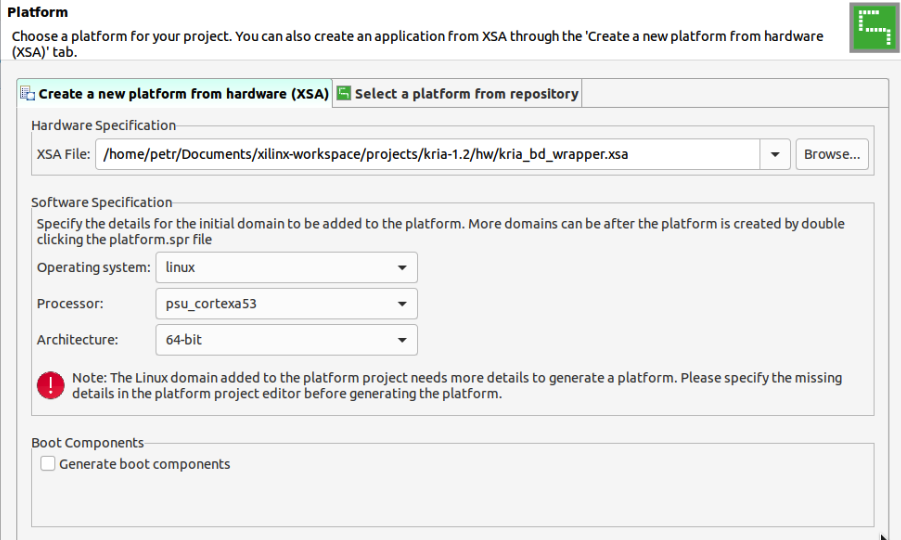
\includegraphics[width=0.75\textwidth]{src/png/vitis-new-platform-linux.png}
			\caption{Xilinx Vitis \gls{abbreviation:ide} – tvorba platformy pro akcelerovanou aplikaci.}
			\label{fig:vitis-new-platform-linux}
		\end{figure}

		\begin{table}[H]
			\centering
			\caption{Nastavení cest souborů pro platformu ve Vitis \gls{abbreviation:ide} v~souboru platform.spr.}
		  \vspace*{0.15cm}
		  \resizebox{\textwidth}{!}
		  {
			\begin{tabular}{!{\vrule width 2pt} l | l | l !{\vrule width 2pt}}
			\noalign{\hrule height 2pt}
			\rowcolor{codeblue}
			Jméno & Cesta & Pozmánka\\
			\noalign{\hrule height 2pt}
			OS & linux & generované automaticky\\ \hline
			Processor & psu\_cortexa53 & generované automaticky\\ \hline
			Supported Runtimes & OpenCL & generované automaticky\\ \hline
			Display Name & linux on psu\_cortexa53 & generované automaticky \\\hline
			Description & linux\_domain & generované automaticky\\ \hline
			BiF File & - & generovat pomocí šipky tlačítka\\ \hline
			Boot components directory & \texttt{<project-name>/linux-files/pfm/boot} & -\\ \hline
			Linux Rootfs & \texttt{<project-name>/<petalinux-project>/images/linux/rootfs.ext4} & generované pomocí \textit{SDK}\\ \hline
			Bootmode & SD & generované automaticky\\ \hline
			FAT32 Partition Directory & \texttt{<project-name>/linux-files/pfm/sd\_card} & složka zůstane prázdná\\ \hline
			Sysroot Directory & \texttt{<project-name>/linux-files/sysroots/cortexa72-cortexa53-xilinx-linux/} & generované pomocí \textit{SDK}\\ \hline
			QEMU Data & - & generované automaticky \\ \hline
			QEMU Arguments & - & generované automaticky \\ \hline
			PMU QEMU Arguments & - & generované automaticky \\\noalign{\hrule height 2pt}
			\end{tabular}
		  }
			\label{tab:vitis-platform-spr-settings}
		\end{table}
		\fbar
		Většinu souborů tvořených ve Vitis je možné otevřít pomocí textového editoru.\\Soubor \texttt{platform.spr} není výjimkou. Pokud dochází k~tvorbě mnoha projektů se stejným nastavením platformy, je možné vytvořit skripty, které automaticky vytvoří konfigurovaný \texttt{platform.spr} soubor s~danou strukturou a nastavením.\par
		Po základní konfiguraci platformy je možné spustit její kompilaci pomocí pravého kliknutí na její název v~okně \textit{Explorer} a volby možnosti \textit{Build Project}. Ukázka tohoto kroku je na obr. \ref{fig:vitis-platform-build}.
		\begin{figure}[htbp!]
			\centering
			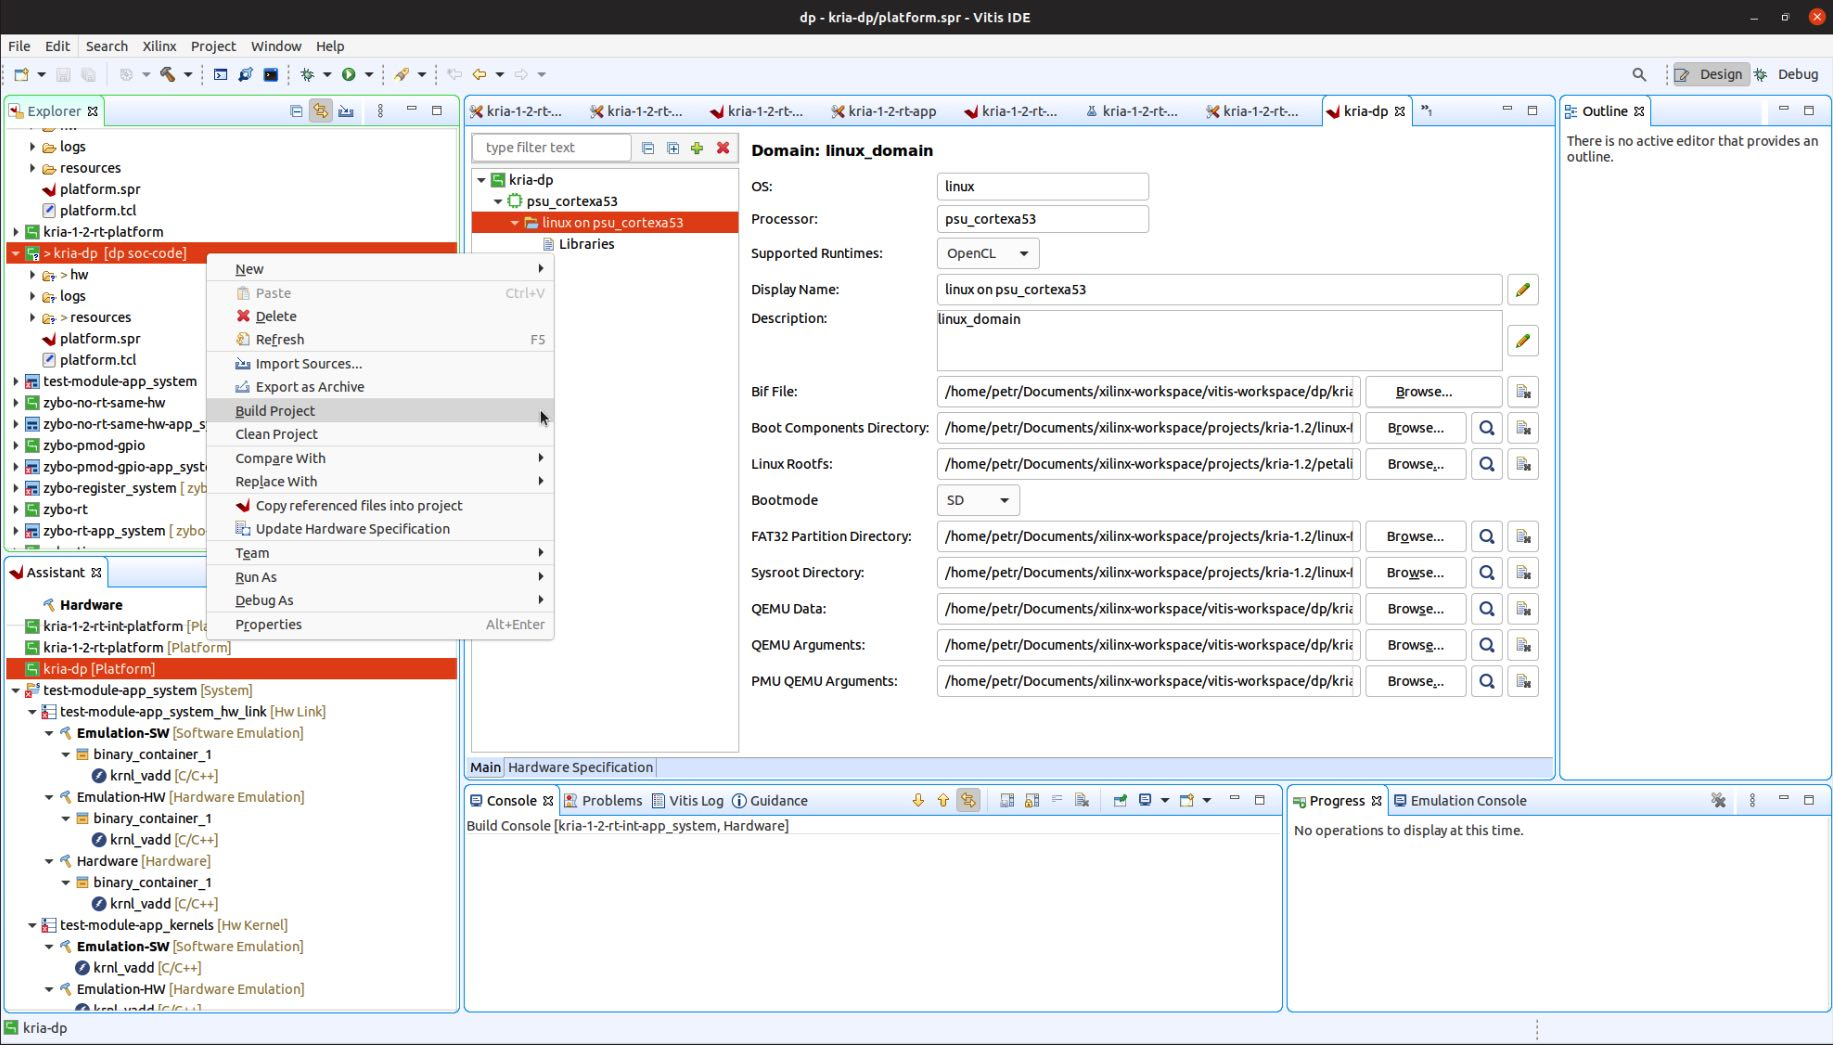
\includegraphics[width=0.95\textwidth]{src/jpg/vitis-build-project-platform.jpg}
			\caption{Xilinx Vitis \gls{abbreviation:ide} – build proces platfromy.}
			\label{fig:vitis-platform-build}
		\end{figure}

		\fbar
		\subsection{Tvorba application project}
		Po dokončení build procesu platformy je již možné přejít k~tvorbě \textit{Application Project}. \textit{Application Project} je možné vytvářet pouze na předem vytvořenou a zkompilovanou platformu. Ukázka výběru platformy s~povolenou \gls{abbreviation:hw} akcelerací, na kterou může být vytvářen \textit{Application Project}, je na obr. \ref{fig:vitis-application-project-platform-selection}.\par
		Při inicializaci projektu v~kroku \textit{Domain} je nutné zvolit v~části \textit{Application settings} cestu k~položce \textit{Kernel Image}, ta je pro vyvíjenou aplikaci umístěna v~cestě\\\texttt{<project-name>/<petalinux-project>/images/linux/Image}.

		\begin{figure}[htbp!]
			\centering
			\includegraphics[width=0.85\textwidth]{src/jpg/vitis-application-project-platform-selection.jpg}
			\caption{Xilinx Vitis \gls{abbreviation:ide} – výběr platformy pro vytvoření Application Project.}
			\label{fig:vitis-application-project-platform-selection}
		\end{figure}

		V~následujícím kroku je doporučeno vytvořit aplikaci z~předpřipravených ukázkových souborů, ze kterých může být aplikace dále rozvinuta dle potřeb. Nejlepším řešením se autorovi jevilo využívat \textit{Simple Vector Addition}. Při využití ukázkových souborů jsou již potřebné části projektu předkonfigurovány a je možné je vhodně upravovat dle požadavků aplikace.\par
		Po načtení ukázkového projektu je možné spustit build proces přímo z~Vitis \gls{abbreviation:ide}, nebo pomocí příkazové řádky. Při realizace této práce bylo využíváno příkazové řádky, protože disponovala rychlejší odezvou na požadovaný build a snadněji se tak aplikace iterovala a vyvíjela.\par
		Aby bylo možné build proces vyvolávat z~příkazové řádky, je nutné vytvořit \texttt{makefile} soubory, které slouží ke kompilaci dílčích zdrojových souborů a k~vyvolání \texttt{v++} linkeru, jež spojí vytvořené dílčí soubory pro \gls{abbreviation:pl} do jednoho binárního souboru \texttt{xclbin}. \texttt{Makefile} soubory je možné vytvořit manuálně, nebo pomocí Vitis \gls{abbreviation:ide} v~okně \textit{Assistant} poklikem pravým tlačítkem myši na název potřebné části a volby \textit{Create Makefiles}.\par
		\vspace*{0.35cm}
		Volbu \texttt{makefiles} je potřeba provést pro složky:
		\begin{enumerate}
			\item \texttt{<application-project-name>\_hw\_link} \textit{[\gls{abbreviation:hw} Link]},
			\item \texttt{<application-project-name>\_kernels} \textit{[\gls{abbreviation:hw} Kernel]},
			\item \texttt{<application-project-name>} \textit{[Host]},
			\item \texttt{<type-of-build>}\\(mimo podsložku, umístěno v~hlavní složce \texttt{<application-project-name>} \textit{[System]}).
		\end{enumerate}
		\vspace*{0.75cm}
		V~některých případech nejsou \texttt{makefile} soubory vytvořeny, nebo aktualizovány dle posledních změn v~projektu. Proto je nutné v~okně \textit{Assistant} pravým tlačítkem kliknout na jednotlivé složky a zvolit \textit{Refresh Project Models} a v~okně \textit{Explorer} zvolit aplikaci a v~nabídce po využití pravého tlačítka myši zvolit \textit{Refresh} a proces generování \texttt{makefile} souborů opakovat.\par
		Struktura \texttt{makefile} souborů je obecná a firma Xilinx dodává na svých stránkách dokumentaci k~jejich tvorbě. V~některých případech, kdy nedocházelo k~jejich automatické aktualizaci, byl autor nucen tyto soubory manuálně upravit. Zejména se úpravy týkaly přidání nových souborů pro generování a linkování objektů pro kernel.\par
		\vspace*{0.35cm}
		% vyřešit mezery mezi původním odstavcem a listem a listem a odstavcem
		Doporučený postup build procesu pro \textit{Hardware} build je následující:
		\begin{enumerate}
			\item build host aplikace pomocí \texttt{makefile} v~cestě\\\texttt{<vitis-workspace>/<application-name>/Hardware/}\\(nejrychlejší proces),
			\item build kernelu pomocí \texttt{makefile} v~cestě\\\texttt{<vitis-workspace>/<application-name>\_kernels/Hardware}\\(středně pomalý proces),
			\item spojování objektů \texttt{xo} z~kroku č. 2 do objektu \texttt{xclbin} pro \gls{abbreviation:pl} pomocí \texttt{makefile} souboru v~cestě\\\texttt{<vitis-workspace>/<application-name>\_system\_hw\_link/Hardware/} (nejpomalejší proces, obsahuje syntézu, implementaci, generování bitstreamu), tento proces u~vytvářené aplikace v~některých případech trval i 1–2 hodiny.
		\end{enumerate}
		\vspace*{0.75cm}
		Dle dostupných informací Xilinx Kria K26 \gls{abbreviation:som} momentálně nepodporuje emulaci. Proto byl představen postup pro \textit{Hardware} build, který je možné aktivovat otevřením konfiguračního souboru \\\texttt{<application-name>\_kernels.prj} v~okně \textit{Explorer}, který se nachází v~cestě\\\texttt{<appliacation-name>\_system/<application-name>\_kernels/}, a výběrem \texttt{Hardware} v~nastavení \textit{Active build configuration}.\par
		Je nutné upozornit, že tento soubor je opět upravitelný v~textovém editoru a této skutečnosti bylo při realizace aplikace velmi využíváno. Soubor obsahuje nastavení jednotlivých akcelerovaných funkcí, výběr optimalizace build procesu a nastavení šířky portu pro přenos dat mezi \gls{abbreviation:ps} a \gls{abbreviation:pl} akcelerovanou funkcí. V~případě, že jsou přidávány do projektu další akcelerované funkce, pro jejich zkompilování je nutné zvolit odpovídající funkce v~tomto souboru pomocí \gls{abbreviation:gui} nabídky. Ovšem v~některých případech nedochází ke správné indexaci souborů ze strany Vitis \gls{abbreviation:ide} a je nutné upravit soubor v~textovém editoru.\par

		

	
	\section{Deployment aplikace na platformu}
	Po úspěšném dokončení build a linking procesu aplikace ve Vitis, je možné přistoupit k~procesu \textit{deployment} (nasazení) aplikace do systému vývojové desky.\par
	Z~kroku \hyperref[subsubsec:konfigurace-device-tree]{\textit{Konfigurace Device Tree}} byl získán soubor \texttt{pl.dtbo}, který byl překopírován do složky \texttt{transfer}, definované v~\hyperref[sec:struktura-slozek]{\textit{Struktura složek}}. Do téže složky je nyní možné překopírovat soubory aplikace:
	\begin{itemize}
		\item \texttt{<application-name>/Hardware/<application-name>} (host program),
		\item \texttt{<application-name>\_system\_hw\_link/\\Hardware/<binary-container>.xclbin} (\gls{abbreviation:pl} bitstream),
	\end{itemize}
	% vyřešit mezery mezi původním odstavcem a listem a listem a odstavcem
	které byly získány z~build procesu pomocí Vitis.\par
	% Info o shell.json
	Aby bylo možné využívat příkazy \texttt{xmutil}, které využívají \texttt{DFX-MGR} (daemon) \cite{xilinx-github-dfx-mgr} pro konfiguraci \gls{abbreviation:pl}, loading a unloading bitstreamů, spravování data modelu daných bitstreamů apod. je třeba pro akcelerovanou aplikaci vytvořit metadata soubor \texttt{shell.json}. Podpora dalších formátů \texttt{shell\_type}, než jen \texttt{XRT\_FLAT} je ve vývoji. \cite{xilinx-github-vitis-tutorials-step-2-create-the-software-components}\par
	Soubor \texttt{shell.json} je opět vhodné vytvořit na vývojářském \gls{abbreviation:pc} a přemístit do složky \texttt{transfer}.\par

	\begin{lstlisting}[language={json}, caption={Metadata shell.json soubor pro xmutil.}, label={lst:metadata-shell-json}]
{
	"shell_type": "XRT_FLAT",
	"num_slots": "1"
}\end{lstlisting}
	
	\vspace*{0.35cm}
	Před přesunem souborů aplikace do vývojové desky obsahuje složka \texttt{transfer} soubory:
	\begin{itemize}
		\item \texttt{pl.dtbo} (Device Tree Blob Object),
		\item \texttt{shell.json} (metadata soubor),
		\item \texttt{<application-name>} (aplikace pro \gls{abbreviation:ps}),
		\item \texttt{<binary-container.xclbin>} (bitstream pro \gls{abbreviation:pl}). 
	\end{itemize}
	\vspace*{0.75cm}

	Bylo zjištěno, že nejrychlejším a nejefektivnějším způsobem pro přenos souborů mezi systémem, na kterém je aplikace vyvíjena (či je třeba data z~aplikace zpracovávat), a systémem vývojové desky (\textit{PetaLinux}) je použití \texttt{\gls{abbreviation:scp}} (secure copy) přes interface \texttt{eth0}.\par
	Příkaz přenosu potřebných souborů pro běh akcelerované aplikace ze složky \texttt{transfer} do složky \texttt{/home/petalinux} na K26 je v~kódu \ref{lst:scp-application-to-kria}.\par
	Dle dostupné dokumentace operačních systémů Linux a macOS bylo zjištěno, že pokud systém vývojového \gls{abbreviation:pc} využívá OpenSSH verze 9.0 a vyšší, je pro přenos souborů pomocí \texttt{\gls{abbreviation:scp}} výchozím protokolem \gls{abbreviation:sftp}. Bez dodatečného nastavení \textit{PetaLinux} by tudíž nebylo možné pouze pomocí \texttt{\gls{abbreviation:scp}} příkazu přenášet soubory. Proto je nutné využít tzv. \textit{legacy \gls{abbreviation:scp} protocol}, aktivovaný pomocí \texttt{-O} v~příkazu \texttt{scp} (\ref{lst:scp-application-to-kria}).\par

	\begin{lstlisting}[language={sh}, caption={Příkaz pro přesun souborů pomocí \gls{abbreviation:scp} ze systému, kde byla aplikace vyvíjena do systému PetaLinux na K26 SOM.}, label={lst:scp-application-to-kria}, morekeywords={scp}]
scp -O pl.dtbo shell.json <application-name> <binary-container.xclbin> root@<ip-address-of-eth-interface>:/home/petalinux
\end{lstlisting}

	Pro práci na vývojové desce v~systému \textit{PetaLinux} autor doporučuje využívat \textit{ssh} a komunikaci přes \gls{abbreviation:usb}/\gls{abbreviation:uart} používat pouze jako prostředí pro výpis informací z~\textit{kernel ring bufferu}, které nejsou pomocí \textit{ssh} bez použití \texttt{dmesg} uživateli viditelné.\par
	Aby došlo k~funkčnímu nakonfigurování\gls{abbreviation:pl} pomocí bitstreamu, je třeba přejmenovat soubor\\\texttt{<binary-container.xclbin>} na \texttt{<binary-container.bin>} (např. pomocí příkazu \texttt{mv}). Pokud by nedošlo k~přejmenování, byla by vypsána chybová hláška.\par
	Pro spuštění akcelerované aplikace \texttt{dfx-mgr} vyžaduje, aby bitstream a soubory aplikace byly vloženy do cesty \texttt{/lib/firmware/<company-name>/<application-name>}. Do verze \textit{PetaLinux} 2022.1 je podporován pouze název \texttt{xilinx} jako \texttt{<company-name>}, od verze 2022.1 jsou podporovány volitelné názvy, ovšem musí být vloženy do souboru \texttt{daemon.config},\\umístěného v~\texttt{/etc/dfx-mgrd/daemon.conf}. \cite{xilinx-github-vitis-tutorials-step-2-create-the-software-components} \cite{xilinx-github-dfx-mgr}\par
	Příkaz pro tvorbu složky \texttt{<application-name>} a pro kopírování požadovaných souborů je zobrazen v~\ref{lst:cp-application-to-firmware}.\par

	\begin{lstlisting}[language={sh}, caption={Příkaz vytvoření potřebné složky aplikace a kopírování potřebných souborů firmwaru.}, label={lst:cp-application-to-firmware}, morekeywords={mkdir, cp}]
mkdir -p /lib/firmware/xilinx/<application-name>

cp pl.dtbo <application-name> <binary-container.bin> shell.json /lib/firmware/xilinx/<application-name>\end{lstlisting}
	
	Následně je možné provést unloading stávající aplikace a loading aplikace \texttt{<application-name>}. Potřebné příkazy s~komentáři jsou zobrazeny v~\ref{lst:xmutil-unloadapp-listapps-loadapp}.\par

	\begin{lstlisting}[language={sh}, caption={Příkaz vytvoření složky aplikace a kopírování potřebných souborů firmwaru.}, label={lst:xmutil-unloadapp-listapps-loadapp}, morekeywords={xmutil}]
xmutil unloadapp # unloading currently active application

xmutil listapps # list currently available applications

xmutil loadapp <application-name> # load user defined application
\end{lstlisting}

Po načtení aplikace je možné ve výpisu \texttt{dmesg} nebo \gls{abbreviation:usb}/\gls{abbreviation:uart} pozorovat, zda došlo ke správnému načtení bitstreamu, zařízení, přiřazení přerušení apod.\par
Aplikaci a bitstream které jsou aktuálně načtené je možné spustit i mimo \texttt{firmware} cestu. Autor doporučuje mít ponechané kopie aplikací v~uživatelské složce\\\texttt{/home/petalinux/<application-name>} a spouštět aplikace příkazem uvedeným v~\ref{lst:petalinux-run-application}.\par


	\begin{lstlisting}[language={sh}, caption={Příkaz pro spuštění akcelerované aplikace.}, label={lst:petalinux-run-application}]
./<application-name> <binary-container.bin>\end{lstlisting}

	V~této části byl představen doporučený postup deploymentu aplikace na zařízení Kria K26 \gls{abbreviation:som}. Postup byl doplněn o~užitečné příkazy a poznámky, které spuštění aplikace urychlují, usnadňují a nebo přinášejí možnost automatizace pomocí \texttt{bash} skriptů.\par
	S~určitou pravděpodobností existují i jiné způsoby deploymentu aplikací, ale autor je v~době realizace této práce zatím nenalezl.


	\fbar
\section{Popis pracoviště}\label{sec:popis-pracoviste}
	Na obr. \ref{fig:workspace-scheme} je zobrazeno blokové schéma pracoviště, které bylo vytvořeno v~rámci této práce a slouží k~vývoji akcelerovaných aplikací.\par
	Blok \textit{\gls{abbreviation:pc}} představuje osobní počítač, který slouží k~přístupu k~pracovišti a je propojeno s~vývojovou deskou KR260 pomocí \textit{\gls{abbreviation:usb}/\gls{abbreviation:uart}} spojení, které je vhodné v~případě, že nedošlo k~inicializaci ethernet adaptéru. Vývojová deska je pomocí adaptéru \textit{eth0} připojena do switche na pracovišti, ke kterému je uživatelský počítač také připojen. Pomocí \textcolor{ctublue}{modrého značení} jsou do switche připojeny také bloky \textcolor{ctuorange}{development machine}. Fyzicky se jedná o~připojení serveru pomocí adaptéru \textit{eno2}, který je umístěn ve fakultním datacentru. Tímto způsobem je vytvořena virtuální síť, která je využívána pouze pro komunikaci mezi zařízeními vývojového pracoviště.\par
	Připojení serveru pomocí adaptéru \textit{eno1} do externí sítě \textcolor{ctugreenyblue}{Ethernet (world)} přináší krom možnosti vzdáleného přístupu do virtualizovaného zařízení v~hypervisoru Proxmox \gls{abbreviation:ve} také možnost vzdáleného přístupu do sítě \textcolor{ctublue}{Ethernet (private)}. Využití serveru pro tvorbu aplikací bylo zvoleno z~důvodu výkonové a časové náročnosti tvoření \textit{PetaLinux} systému, \gls{abbreviation:hw} designu ve Vivado a tvoření bitstreamu ve Vitis \gls{abbreviation:ide}. Díky vzdáleným přístupům je možné pracovat na vývoji i mimo laboratoř. Protože v~některých případech při restartování vývojové desky nedochází ke správné inicializaci adaptéru \textit{eth0}, je v~navazující práci plánováno připojit vývojovou desku k~\gls{abbreviation:sbc} (single board computer) pomocí \textit{\gls{abbreviation:usb}/\gls{abbreviation:uart}} rozhraní a \gls{abbreviation:sbc} připojit do \textcolor{ctublue}{Ethernet (private)}. K~vývojové desce bude možné přistupovat cestou \textcolor{ctugreenyblue}{Ethernet (world)} -> \textcolor{ctuorange}{development machine} -> \textcolor{ctublue}{Ethernet (private)} -> \gls{abbreviation:pcb} -> \textit{\gls{abbreviation:usb}/\gls{abbreviation:uart}} -> Kria KR260. Toto fyzické spojení umožní přístup ke K26 pomocí \textit{minicom}. Po přípojení bude možní provést manuální inicializaci adaptéru po restartování vývojové desky.\par
	Protože ukázka využití \gls{abbreviation:spi} komunikace je realizována pomocí obvodu \textit{MAX7219} s~\gls{abbreviation:led} maticí, který vyžaduje napájení v~rozmezí 4~V~až 5~V~a výstupy \gls{abbreviation:pmod} dodávají napětí pouze 3,3~V, je třeba pro napájení testovacího rozhraní využít externího zdroje. V~této práci byla pro napájení obvodu využita deska Arduino UNO, která je napájena z~\gls{abbreviation:usb} rozhraní uživatelského počítače. Volba tohoto napájení byla vybrána z~důvodu jednoduchosti a dostupnosti. Provedení zapojení pro testování \gls{abbreviation:spi} komunikace je znázorněno v~části \hyperref[subsubsec:zapojeni-pro-testovani-spi-komunikace]{\textit{Zapojení pro testování SPI komunikace}}.\par
	Představená architektura pracoviště byla tvořena tak, aby nebylo problematické ji rozšiřovat o~další prvky a umožňovala vzdálený přístup s~podporou více aktivních uživatelů v~jeden okamžik.


\begin{figure}[htbp!]
	\centering
	\includegraphics[width=0.95\textwidth]{src/pdf/workspace-scheme.pdf}
	\caption{Blokové schéma uspořádání vývojového pracoviště.}
	\label{fig:workspace-scheme}
\end{figure}

	\fbar

\section{Vytvořená aplikace}\label{sec:vytvorena-aplikace}
 V~této části je představena vytvořená aplikace pro \gls{abbreviation:ps} a akcelerovaná aplikace pro \gls{abbreviation:pl}. Shodnocení výsledků aplikací je uvedeno v~sekci \hyperref[sec:poznatky-ziskane-profilovanim-aplikaci]{\textit{Poznatky získané profilováním aplikací}}.\par
 Hlavním cílem této práce bylo představit možnosti využití platformy pro řízení elektrického pohonu nebo systém \gls{abbreviation:hil}. Proto jednotlivé ukázkové podaplikace reprezentují části a algoritmy, které by bylo možné využít při realizaci skutečného připojení platformy k~řízenému pracovišti.\par
 % přidat odkaz na místo, kde budou časové výsledky, ukázky z vitis analyzéru apod.
 Aby bylo možné představit jednotlivé funkce, které by byly používány při řízení elektrického pohonu, je ukázková aplikace rozdělena do pěti větví, které je možné vybrat po spuštění aplikace. Je nutné podotknout, že větev \texttt{PRELOADED DATA} bylo nutné realizovat do zvláštní aplikace, protože současné vkládání všech vytvořených kernelů do bitstreamu by vyžadovalo příliš mnoho resources (např. \gls{abbreviation:fifo}). Aby bylo možné všechny větve aplikace realizovat s~pomocí pouze jednoho bitstreamu, bylo by nutné podrobit algoritmus kernelu další optimalizaci.\par
 Základních pět větví ukázkové aplikace a jejich vztahy k~celkovému běhu programu jsou zobrazeny na obr. \ref{fig:application-overview}.

 \begin{figure}[htbp!]
	\centering
	\includegraphics[width=1\textwidth]{src/pdf/application-overview.pdf}
	\caption{Základní větvení ukázkové aplikace.}
	\label{fig:application-overview}
\end{figure}
	Po spuštění hlavního procesu je pomocí \texttt{selectionMode} proměnné možné volit, jaká podaplikace bude spuštěna. Následně je provedena dynamická alokace paměti pro využívané struktury a pole v~daných aplikacích. Je nutné zmínit, že \texttt{PRELOADED DATA} aplikace využívá unikátní sadu proměnných, které nejsou využívány v~ostatních aplikacích. Z~tohoto důvodu obsahuje \texttt{PRELOADED DATA} samostatnou skladbu instrukcí pro dealokaci paměti. Jednotlivé podaplikace jsou představeny v~následujících částech práce pomocí názorných vývojových diagramů.\par
	Po ukončení podaplikací jsou vyvolány příkazy pro dealokaci paměti, která byla alokována dynamicky v~programu \gls{abbreviation:ps}.\par
	\fbar

	\subsection{Bezpečnost při uživatelském ukončení aplikace}
	Z~důvodu bezpečnosti je do algoritmu aplikace zakomponována funkce \texttt{signal\_callback\_handler}, jež reaguje na signál \texttt{SIGINT}. Tento signál je momentálně vysílán v~případě přerušení běhu aplikace uživatelem. Handler funkce je registrována na signál již na počátku hlavní \texttt{main(int argc, char *argv[])} funkce aplikace.\par
	V~kódu č. \ref{lst:signall-callback-handler} je představana deklarace struktury typu \texttt{InvertorSwitchType}, která slouží k~uložení hodnot stavu virtuálních spínačů invertoru. Poté následuje deklarace funkce \texttt{stopInvertor()}, která po vyvolání nastaví stavy všech virtuálních spínačů na \texttt{0} a zajistí vypsání informační hlášky ohledně tohoto děje pro případ debuggingu.\par
	Funkce \texttt{signal\_callback\_handler} vypisuje hlášku o~zachycení \texttt{SIGINT} signálu, zajišťuje spuštění funkce \texttt{stopInvertor()} a ukončení programu.

	\begin{lstlisting}[language={c++}, caption={signal\_callback\_handler funkce a její registrace na signál SIGINT.}, label={lst:signall-callback-handler}]
// main.cpp
InvertorSwitchType invertorSwitchGlobal;

void stopInvertor()
{
    invertorSwitchGlobal.sw1 = 0;
    invertorSwitchGlobal.sw2 = 0;
    invertorSwitchGlobal.sw3 = 0;
    invertorSwitchGlobal.sw4 = 0;
    invertorSwitchGlobal.sw5 = 0;
    invertorSwitchGlobal.sw6 = 0;

    std::cout << "Set all invertor switches at 0!\n";
}


// Define the function to be called when ctrl-c (SIGINT) is sent to process
void signal_callback_handler(int signum)
{
    std::cout << "\nCaught signal " << signum << "\n";

    // stoping invertor of global variables
    stopInvertor();
    std::cout << "Terminating program!\n";
    // Terminate program
    exit(signum);
}// Define the function to be called when ctrl-c (SIGINT) is sent to process
void signal_callback_handler(int signum)
{
    std::cout << "\nCaught signal " << signum << "\n";

    // stoping invertor of global variables
    stopInvertor();
    std::cout << "Terminating program!\n";
    // Terminate program
    exit(signum);
}

// main.cpp
main(int argc, char *argv[])
{
	// Register signal and signal handler
	signal(SIGINT, signal_callback_handler);
.
..
...
}\end{lstlisting}

	\fbar
	\subsection{Keyboard Input}\label{subsec:keyboard-input}
		Program, který je v~podaplikaci \textit{Keyboard Input} akcelerován v~\gls{abbreviation:pl}, se nazývá kernel. (v~tomto kontextu není myšleno jádro systému Linux) Tento kernel je realizován v~\gls{abbreviation:pl} a jeho úkolem je provést časově náročné výpočty. V~podaplikaci \textit{Keyboard Input}, \hyperref[subsec:cpu-fpga]{\textit{CPU/FPGA Model}} a \hyperref[subsec:preloaded-data]{\textit{Preloaded Data}} byl v~\gls{abbreviation:pl} realizován matematický $I$-$n$ model asynchronního motoru, regulace a Space Vector Modulation (\gls{abbreviation:svm}). Hlavním výstupem kernelu jsou virtuální stavy sepnutí spínačů, které by v~reálné aplikaci byly napojeny na fyzické piny \gls{abbreviation:pmod} a ovládaly by drivery řízených výkonových polovodičových prvků měniče.\par
		Naznačený algoritmus aplikace je zobrazen na obr. \ref{fig:keyboard-input}. Akcelerované aplikace v~této práci obsahují totožné inicializační a deinicializační funkce.\par
		\subsubsection{Konfigurace PL}
		Blok \texttt{\gls{abbreviation:pl} SETTINGS PREAMBLE} obsahuje kód, jehož předloha byla získána z~ukázkových souborů akcelerovaných aplikací přímo v~aplikaci Vitis. V~tomto bloku dochází k~inicializaci \gls{abbreviation:pl} zařízení, definování příkazové fronty (Command Queue), programu pro \gls{abbreviation:pl}, platformy a k~definici kernelů. Funkce a definice typů, jež jsou použity pro jednotlivé proměnné jsou pro akcelerované aplikace definovány v~\texttt{cl2.hpp} knihovně. V~preambuli se nachází smyčka, jež vyhledává platformy zařízení Xilinx a pokud dojde k~jejímu úspěšnému nalezení, pokouší se algoritmus do ní nahrát bitstream ve formátu \textit{xclbin} nebo \textit{bin}. Po úspěšném nahrání bitstreamu, jsou deklarovány potřebné elementy pro spouštění kernelu. (Context, CommandQueue, Program, Kernel). Veškeré funkce, jež využívají \textit{openCL} knihovny, jsou uzavřeny do definovaného makra, které v~případě, že vykonávaný příkaz navrátí jinou návratovou hodnotu než \texttt{CL\_SUCCESS} (0), vypíše informace o~dané chybě. Toto makro není podstatné pro funkční aplikaci, ovšem je velmi vhodné pro možný debugging. Definice makra byla také převzata z~ukázkových akcelerovaných aplikací.

		\subsubsection{PS Aplikace}
			Pokud průchod aplikace částmi pro inicializaci a konfiguraci \gls{abbreviation:pl} byl úspěšný, aplikace přecházi do části, ve které jsou definovány a deklarovány parametry pro simulaci, pro $I$-$n$ model motoru a pro regulaci. V~části \texttt{PARAMETERS SETTINGS} dochází k~dynamické alokaci paměti pomocí \texttt{posix\_memalign()} funkce. U~některých parameterů je při jejich definici znán jejich počet, proto by bylo možné použít statické alokace paměti. Ovšem pro demonstraci práce s~\texttt{posix\_memalign()} byl zvolen přístup dynamické alokace. Při použití dynamické alokace je nutné provést zarovnání paměti na 4096 bitů, \par
			Následně je uživatel tázán o~jakou podaplikaci má zájem, po zadání čísla, odpovídající dané podaplikaci \texttt{KEYBOARD INPUT} je uživatel tázán ohledně vstupních hodnot do $I$-$n$, které jsou pomocí funkce \texttt{scanf()} vloženy do odpovídajících proměnných.\par
			V~algoritmu je dále uveden blok \texttt{MASTER INPUT PREP}, který reprezentuje přípravu datového pole typu \textit{float}, které je využito k~přesunu dat do globální paměti. Z~globální paměti jsou data využívána akcelerovaným kernelem. Je možné přenéšet do globální paměti i více vstupních proměnných, které budou ukládány do globální paměti, ovšem poté je v~kernelu nutné vytvořit více interfaces. Větší množství rozhraní je třeba, aby bylo možné data načítat paralelně a urychlit tím dobu vykonávání kernelu. Při zkoumání využitelnosti platformy v~této práci byl ovšem vliv rozdělení jedotlivých interfaces na rychlost vykonávání minimální. Vznikl však rozdíl ve využitých resources. Pokud se v~platformě Digilent Zybo využilo více interfaces a bylo požadováno paralelní načítání dat kernelem, měl tento požadavek v~některých případech za následek nemožnost umístění designu na \gls{abbreviation:pl}, protože bylo překročeno maximálního počtu využitých resources.\par
			
			\subsubsection{Interakce s~kernelem}
			Po přípravě proměnné \texttt{masterInput} je do CommandQueue pro dané zařízení vložen požadavek na přesun proměnných v~podobě vytvořeného bufferu do globální paměti, přístupné \gls{abbreviation:pl}. Po ukončení přenosu bufferů do paměti, je možné do CommandQueue zařadit požadavek na spuštění kernelu\\\texttt{krnl\_calculateCurVelModel}. Pokud dojde k~úspěšnému vykonání kernelu, je možné přesunout výsledné hodnoty uložené v~bufferu z~globální paměti do paměti \gls{abbreviation:ps} pomocí příkazu\\\texttt{enqueueMigrateMemObjects}. Část reprezentující komunikaci s~kernelem, ohraničená na obr. \ref{fig:keyboard-input} přerušovanou křivkou, je zobrazena v~kódu \ref{lst:interakce-s-krnl-calculateCurVelModel}. Postup interakce s~tímto kernelem je totožný i v~podaplikacích \hyperref[subsec:cpu-fpga]{\textit{CPU/FPGA Model}} a \hyperref[subsec:preloaded-data]{\textit{Preloaded Data}}. Interakce s~kernelem \texttt{krnl\_calculateInvMot} v~podaplikaci \hyperref[subsec:cpu-fpga]{\textit{CPU/FPGA Model}}, která využívá akcelerovaný model asynchronního motoru, je odlišná ve struktuře přenášeného bufferu do a z~globální paměti.\par

 		\begin{figure}[htbp!]
			\centering
			\includegraphics[width=1\textwidth]{src/pdf/keyboard-input.pdf}
			\caption{Keyboard Input větev aplikace – manuální nastavování vstupních hodnot do $I$-$n$ modelu.}
			\label{fig:keyboard-input}
		\end{figure}

		\begin{lstlisting}[language={c++}, caption={Interakce s~kernelem krnl\_calculateCurVelModel.}, label={lst:interakce-s-krnl-calculateCurVelModel}, morekeywords={OCL_CHECK, enqueueMigrateMemObjects, finish, enqueueTask, CL_MIGRATE_MEM_OBJECT_HOST}, literate=
			 {\{}{{{\color{ctured}{\{}}}}{1}
			 {\}}{{{\color{ctured}{\}}}}}{1}
			 {)}{{{\color{ctured}{)}}}}{1}
			 {(}{{{\color{ctured}{(}}}}{1}]
OCL_CHECK(err, err = q.enqueueMigrateMemObjects({buffer_masterInput}, 0 /* 0 means from host*/));
OCL_CHECK(err, q.finish());

OCL_CHECK(err, err = q.enqueueTask(krnl_calculateCurVelModel));
OCL_CHECK(err, q.finish());

OCL_CHECK(err, q.enqueueMigrateMemObjects({buffer_masterOutput}, CL_MIGRATE_MEM_OBJECT_HOST));
OCL_CHECK(err, q.finish());
\end{lstlisting}

	Po přesunu dat z~globální paměti je vybraná sada hodnot proměnných vypsána uživateli v~konzoli. Nyní by bylo možné program ukončit, ale pro demonstraci funkce aplikovaného \gls{abbreviation:rt}, je znovu deklarován vstupní vektor proměnných a opět je kernel spuštěn. Pokud jsou výsledky získané z~akcelerovaného kernelu totožné s~předchozí iterací, došlo ke správné aplikaci \gls{abbreviation:rt} patche.\par
	Na počátku vývoje a debuggování aplikace, kdy nebyl \gls{abbreviation:rt} patch využit, vznikal problém nekonzistentnosti výsledků mezi iteracemi. Více o~problematice \gls{abbreviation:rt} patche je uvedeno v~části \hyperref[subsec:real-time-linux-patch]{\textit{RealTime Linux Patch}}.\par
	Na závěr dojde k~odmapování bufferů od přidružených ukazatelů, které byly využity pro interakci s~kernelem. Program je zakončen uvolněním využité paměti, dynamicky alokované v~předchozích krocích.\par
	V~obr. \ref{fig:keyboard-input-terminal} je možné pozorovat snímek konzole/terminálu, který zachycuje postup přihlášení pomocí \texttt{\gls{abbreviation:ssh}} k~vývojové desce s~K26, unload stávající aplikace, loading uživatelské aplikace \texttt{rt} a její následné spuštění. Dále je zobrazen výběr podaplikace a výpis vybraných hodnot proměnných po první iteraci kernelu.

	\begin{figure}[htbp!]
		\centering
		\includegraphics[width=1\textwidth]{src/png/keyboard-input-terminal.png}
		\caption{Snímek obrazovky konzole, zobrazující postup spuštění podaplikace \hyperref[subsec:keyboard-input]{Keyboard Input} a výpis první iterace výsledků z~kernelu.}
		\label{fig:keyboard-input-terminal}
	\end{figure}

		\fbar
		\subsection{CPU/FPGA Model}\label{subsec:cpu-fpga}
			Nejrozsáhlejší částí hlavního programu je podaplikace s~názvem \gls{abbreviation:cpu}/\gls{abbreviation:fpga} Model, která využívá dvou kernelů, které komunikují přes \gls{abbreviation:ps}. Při prozkoumávání využití platformy autor narazil na možnost, že by kernely streamovaly data přímo mezi sebou, bez nutnosti použití \gls{abbreviation:ps}. Tento způsob přenosu dat nebyl v~této práci využit, ale je plánováno jeho testování. Tyto kernely by bylo také vhodné realizovat stylem \textit{free running}, kdy by data byla z~\gls{abbreviation:ps} streamovaná přímo do jednotlivých kernelů v~okamžiku, když by byla v~\gls{abbreviation:ps} k~dispozici. To by nejspíše umožnilo rychlejší reakci kernelu, která by přinesla zkrácení doby potřebné na přesun dat z~\gls{abbreviation:ps} do \gls{abbreviation:pl} a naopak. Experimentálně zjištěné časy a timeline graf je uveden v~sekci \ref{subsec:poznatky-ziskane-profilovanim-aplikaci-cpu-fpga}\par
			% dodat odkaz na sekci, kde budou umístěné výsledky
			Algoritmus, využívaný v~této práci, je uveden na obr. \ref{fig:cpu-fpga-model}.\par
			K~inicializaci PL je využita totožná preambule jako v~\hyperref[subsec:keyboard-input]{\textit{Keyboard Input}} podaplikaci. Stejným způsobem dochází i k~inicializaci potřebných bufferů a k~nastavení parametrů modelů a simulace.\par
			Protože dochází k~modelování i regulátorů, je v~případě této podaplikace důležité nastavit žádané hodnoty regulovaných veličin. V~této ukázkové aplikaci jsou žádané hodnoty mechanické otáčivé rychlosti \gls{symbol:mechanicka-uhlova-rychlost} a velikosti magnetického toku rotoru \gls{symbol:psi2} nastaveny přímo v~kódu aplikace. V~případě realizace skutečné regulace by bylo vhodné disponovat možností měnit tyto hodnoty v~průběhu běhu programu pomocí konzole, nebo pomocí externího zařízení, komunikující s~platformou pomocí \gls{abbreviation:spi} nebo jiného druhu komunikace.\par
			Před spuštěním smyčky, která zajišťuje hlavní iteraci programu, je v~programu zařazeno vytvoření souboru \texttt{globalSimulationData.csv}, který slouží k~uchování hodnot vybraných sledovaných veličin. Soubor je dále využíván při tvorbě výsledných grafů simulace pomocí Python skriptu. Výsledný graf simulace a důvod využití skriptu je uveden v~části \hyperref[subsubsec:zobrazeni-vysledku-simulace]{\textit{Zobrazení výsledků simulace}}.\par
			V~programu následuje blok označený \texttt{krnl\_calculateCurVelModel}, jež rezprezentuje interakci s~kernelem. Po migraci hodnot veličin z~globální paměti do paměti \gls{abbreviation:ps} je možné získané výsledky vypsat do konzole. Po provedení kernelu, obsahující $I$-$n$ model, bloky regulace a algoritmus \gls{abbreviation:svm}, jsou získané stavy virtuálních spínačů vloženy do vstupního vektoru pro kernel \texttt{krnl\_calculateInvMot}. Tento kernel obsahuje modely invertoru a asynchronního motoru, popsaného v~části \hyperref[sec:model-stroje]{\textit{Model stroje}}. Po úspěšném provedení kernelu a získání vypočtených hodnot z~globální paměti jsou hodnoty některých významných veličiny pro čtyři první iteraci algoritmu vypsány v~konzoli. Vybrané veličiny, u~kterých je vhodné sledovat jejich závislost na čase, jsou vloženy do souboru \texttt{globalSimulationData.csv} pro další zpracování. Následuje uzavření aktivního souboru a dealokace paměti použitých proměnných a bufferů.

			\begin{figure}[htbp!]
				\centering
				\includegraphics[width=1\textwidth]{src/pdf/cpu-fpga-model.pdf}
				\caption{\gls{abbreviation:cpu}/\gls{abbreviation:fpga} Model větev aplikace – matematický $I$-$n$ model, regulace, \gls{abbreviation:asm} model v~\gls{abbreviation:fpga}.}
				\label{fig:cpu-fpga-model}
			\end{figure}	 

			\fbar
			\subsubsection{Zobrazení výsledků simulace}\label{subsubsec:zobrazeni-vysledku-simulace}
			Aby bylo možné při debuggingu aplikace vizuálně pozorovat výsledky simulace, bylo nutné data ze souboru \texttt{globalSimulationData.csv} vizualizovat způsobem, jež umožňuje rychlé zpracování velikého množství dat a v~nejlepším případě je Open Source.\par
			První přístup spočíval ke kontrole výsledků v~programu Wolfram Mathematica. Ovšem při kroku simulace 1 $\mu$s a simulovaném čase 1 s~se jednalo o~výpis jednoho milion hodnot. Vykreslení takového množství bodů, které byly přímkově spojeny, bylo příliš náročné pro zařízení autora a trvalo přiliš dlouho dobu. A~protože Wolfram Mathematika vyžaduje licenci, bylo od tohoto způsobu upuštěno. Další možností bylo využití programu MATLAB™, ovšem opět je vyžadována licence a autor dbal na co největší otevřenost projektu. Proto bylo nakonec využito jazyku Python, jež není zatížen problémem \textit{Vendor lock-in} a vykreslení požadovaného grafu se stejnou kvalitou jako v~MATLAB™u nebo ve Wolfram Mathematica trvalo velmi krátkou dobu. Python skript pro vykreslení grafu je součástí přílohy této práce. Graf č. \ref{fig:k26-simulace-graf-mechanicka-rychlost-velikost-mg-toku-rotoru} reprezentuje výsledky simulace řízení asynchronního motoru pomocí \gls{abbreviation:foc}. Zobrazené výsledky odpovídají žádaným hodnotám, regulovaných veličin. V~simulaci byly nastaveny požadované hodnoty:
			\begin{itemize}
				\item velikost magnetického toku rotoru \gls{symbol:psi2} = 0,9032 Wb,
				\item velikost mechanické otáčivé rychlosti \gls{symbol:mechanicka-uhlova-rychlost} = 10 s$^{-1}$ v~čase \gls{symbol:t-cas} = 0,6 s.
			\end{itemize}

			


		\begin{figure}[htbp!]
			\centering
			\includegraphics[width=1\textwidth]{src/pdf/k26-simulace-graf-mechanicka-rychlost-velikost-mg-toku-rotoru.pdf}
			\caption{Časová závislost velikosti mechanické otáčivé rychlosti \gls{symbol:mechanicka-uhlova-rychlost} a velikosti magnetického toku rotoru \gls{symbol:psi2}. Výsledné hodnoty získané ze simulace akcelerované pomocí kernelu v~\gls{abbreviation:pl}.}
			\label{fig:k26-simulace-graf-mechanicka-rychlost-velikost-mg-toku-rotoru}
		\end{figure}


		



	   \fbar
	   \subsection{Preloaded Data}\label{subsec:preloaded-data}
	   Podaplikace preloaded data je z~důvodů, popsaných v~sekci \hyperref[sec:vytvorena-aplikace]{\textit{Vytvořená aplikace}}, realizována v~odděleném Application projektu v~programu Vitis.\par
	   Aplikace byla součástí prvních experimentů s~využitím kernelů a proto obsahuje starší (legacy) strukturu algoritmu, včetně legacy kódu v~kernelu, který využívá více vstupních a výstupních vektorů a tudíž i interfaces (z~důvodu testování optimalizace).\par
	   Zjednodušený vývojový diagram aplikace je na obr. \ref{fig:preloaded-data}. Stejně jako pro ostatní představené akcelerované aplikace je na počátku hlavního programu umístěn blok zajišťující inicializaci prvků pro kernel. Hlavním rozdílem od předchozích aplikací je definice a deklarace pouze jediného kernelu\\ \texttt{krnl\_CurVelLoadLegacy}. Ukázka deklarace je v~kódu \ref{lst:krnl-curvelloadlegacy-declaration}.\par
	   \newpage

	   \begin{lstlisting}[language={c++}, caption={Deklarace kernelu krnl\_CurVelLoadLegacy v~podaplikace Preloaded Data.}, label={lst:krnl-curvelloadlegacy-declaration}, morekeywords={OCL_CHECK, enqueueMigrateMemObjects, finish, enqueueTask, CL_MIGRATE_MEM_OBJECT_HOST}, literate=
		{\{}{{{\color{ctured}{\{}}}}{1}
		{\}}{{{\color{ctured}{\}}}}}{1}
		{)}{{{\color{ctured}{)}}}}{1}
		{(}{{{\color{ctured}{(}}}}{1}]
OCL_CHECK(err, krnl_CurVelLoadLegacy = cl::Kernel(
	program, "krnl_CurVelLoadLegacy", &err));
\end{lstlisting}
	Po potřebných deklaracích a definicích, nutných pro správnou funkci kernelu, je dynamicky naalokována paměť pro vybrané konstatní parametry simulace. Tyto parametry jsou např. krok simulace, časové rozmezí simulace či počet kroků. Protože je v~podaplikaci simulován zjednodušený $I$-$n$ model, kdy není uvažována změna parametrů stroje během simulace (např. rezistivita rotorového vinutí), jsou v~bloku \texttt{PARAMETERS SETTINGS} definovány také parametry stroje vstupující do myšleného modelu.\par
	Do této aplikace vstupují předpočítané nebo změřené hodnoty následujících veličin:
	\begin{itemize}
		\item proud \gls{symbol:i1-velikost-program}, jež reprezentuje velikost proudu statoru \gls{symbol:i1a} procházející první fází do řízeného motoru,
		\item proud \gls{symbol:i2-velikost-program}, jež reprezentuje velikost proudu statoru \gls{symbol:i1b} procházející druhou fází do řízeného motoru,
		\item proud \gls{symbol:i3-velikost-program}, jež reprezentuje velikost proudu statoru \gls{symbol:i1c} procházející třetí fází do řízeného motoru,
		\item mechanická otáčivá rychlost rotoru mototu \gls{symbol:mechanicka-uhlova-rychlost}.
	\end{itemize}
	Uvedené hodnoty jsou načítány ze souboru \texttt{outputData.csv}, který je strukturován dle formátu uvedeného v~\ref{lst:output-data-csv-struktura}. Formát nevyužívá nových řádků pro oddělení sady dat, pouze využívá oddělení pomocí čárky. Tento formát byl zvolen z~důvodu, aby byla zajištěna co nejmenší velikost souboru a aby bylo maximálně zjednodušeno načítání dat pomocí funkce \texttt{std::getline}.\par

	\begin{lstlisting}[language={Text}, caption={Struktura souboru outputData, ze kterého jsou načítány hodnoty pro akcelerovaný kernel.}, label={lst:output-data-csv-struktura}]
time,i1,i2,i3,MechanicalAngularVelocity.,..,...
\end{lstlisting}
	Po načtení hodnot do definovaných proměnných jsou vytvořeny v~\gls{abbreviation:ps} buffery, které jsou mapovány na adresy odpovídajících ukazatelů a mají rozsah jednotlivých proměnných, ke kterým jsou mapovány. Buffery jsou nastaveny jako jednotlivé vstupní parametry kernelu.\\Ve vyznačené části \texttt{krnl\_CurVelLoadLegacy} na obr. \ref{fig:preloaded-data} je provedena sada příkazů pro přenos hodnot proměnných pomocí bufferů do globální paměti, přístupné z~\gls{abbreviation:pl}, spuštění kernelu a opětovné přenesení výsledných hodnot z~globální paměti do \gls{abbreviation:ps}.\par
	V~této legacy aplikaci je při výpisu hodnot vybraných veličin také provedeno ukládání hodnot do csv souboru \texttt{outputCurVel2.csv}. Struktura tohoto legacy souboru je v~kódu \ref{lst:output-cur-vel-2-csv}.\par
	Po ukončení podaplikace je opět dealokována paměť proměnných, která byla dynamicky alokována.

	\begin{lstlisting}[language={Text}, caption={Struktura souboru outputCurVel2.csv, do něhož jsou umisťovány výstupní hodnoty vybraných veličin, vypočtených pomocí akcelerované aplikace.}, label={lst:output-cur-vel-2-csv}]
time,psi2Amplitude,transformAngle
.
..
...\end{lstlisting}



		\begin{figure}[htbp!]
		   \centering
		   \includegraphics[width=1\textwidth]{src/pdf/preloaded-data.pdf}
		   \caption{Preloaded Data větev aplikace – automatické čtení změřených/simulovaných vstupních hodnot do $I$-$n$ modelu a jejich hromadné zpracování v~kernelu.}
		   \label{fig:preloaded-data}
	   \end{figure}

	   \fbar
	   \subsection{SPI}\label{subsec:spi}
	   Pro potencionální komunikaci s~externími jednotkami v~reálné aplikaci bylo zvoleno \gls{abbreviation:spi} rozhraní. \gls{abbreviation:spi} bylo zvoleno, protože je využíváno externími jednotkami jako jsou \gls{abbreviation:adc}, \gls{abbreviation:dac}. Tyto jednotky jsou schopny díky \gls{abbreviation:spi} komunikovat s~řídící platformou téměř v~reálném čase.\par
	   Část aplikace, která prezentuje funkčnost \gls{abbreviation:spi} komunikace není oproti předchozím podaplikacím akcelerována. Tudíž nevyužívá akcelerované funkce (kernelu) pro urychlení výpočtů. Využívá však \gls{abbreviation:pl}, ve kterém byl vytvořen \gls{abbreviation:ip} blok \textit{\gls{abbreviation:axi} Quad \gls{abbreviation:spi}}, který umožňuje \gls{abbreviation:spi} komunikaci. Tento blok způsobí vytvoření adres pamětí, které je možní z~userspace programu nebo běhu \textit{PetaLinux} systému adresovat.\par
	   Jiná možná realizace \gls{abbreviation:spi} komunikace by byla pomocí \gls{abbreviation:spi} driveru v~\gls{abbreviation:ps}, který by bylo nutné aktivovat při tvorbě \textit{PetaLinux} systému.\par
	   Je důležité zmínit, že nakonfigurované parametry bloku \textit{\gls{abbreviation:axi} Quad \gls{abbreviation:spi}} lze změnit pouze ve Vivado, tudíž je důležité při tvorbě \gls{abbreviation:hw} platformy již znát požadavky zařízení, se kterými bude aplikace komunikovat. Tyto parametry jsou délka přenášené zprávy nebo frekvenci signálu \texttt{\gls{abbreviation:clk}}.\par
	   
	   \begin{figure}[htbp!]
			\centering
			\includegraphics[width=1\textwidth]{src/pdf/spi.pdf}
			\caption{\gls{abbreviation:spi} větev aplikace – manuální odesílání dat přes \gls{abbreviation:spi}.}
			\label{fig:spi}
	\end{figure}

	Pro zjednodušení adresování \gls{abbreviation:spi} registrů jsou v~aplikaci definovány posuny od základní adresy pomocí \texttt{define} direktiv. Definice direktiv dle dokumentace \cite{axi-quad-spi-ip-product-guide} je zobrazena v~\ref{lst:define-direktivy-spi}.\par

	\fbar
	\begin{lstlisting}[language={c++}, caption={Definice posuvu adres pro registry \gls{abbreviation:axi} Quad \gls{abbreviation:spi} bloku pomocí define direktiv.}, label={lst:define-direktivy-spi}]
#define MAP_SIZE 0x10000
#define SPI_SPICR 0x60
#define SPI_SPISR 0x64
#define SPI_DTR 0x68
#define SPI_DRR 0x6C
#define SPI_SPISSR 0x70
#define SPI_TRANSMIT_FIFO_OCUPANCY 0x74
#define SPI_RECEIVE_FIFO_OCUPANCY 0x78
#define SPI_DGIER 0x1C
#define SPI_IPISR 0x20
#define SPI_IPIER 0x28\end{lstlisting}

	Jak je možné na názorném vývojovém diagramu \ref{fig:spi} pozorovat, je pro zvýšení bezpečnosti programu využito mapování pouze potřebné části \gls{abbreviation:hw} registrů. K~mapování do uživatelského prostředí dochází pomocí \gls{abbreviation:uio} zařízení a \texttt{mmap} funkce. V~\gls{abbreviation:dt} jednotky je využit \textit{generic-uio} driver, díky kterému je možné pozorovat vzniklá přerušení od \gls{abbreviation:spi} a tyto přerušení také znovu povolovat pomocí acknowledge operace. Autor zatím nenašel způsob, pomocí něhož by bylo možné vykonat acknowledge přerušení v~\textit{PetaLinux}, pokud by bylo využito výchozích driverů \gls{abbreviation:spi} jednotky.\par
	Po provedení mapování adres registrů do userspace pomocí funkce \texttt{initializeSPI()} (jejíž algoritmus je zobrazen v~kódu \ref{lst:initialize-spi}) následuje inicializace jednotky, se kterou aplikace má komunikovat. Pro ukázku využití \gls{abbreviation:spi} komunikace s~externím prvkem byla realizována komunikace s~jednotkou \textit{MAX7219}, připojenou na LED matici 8x8. Pokud by se jednalo o~aplikaci v~produkčním prostředí elektrických pohonů, probíhala by komunikace nejspíše s~analogově-digitálními převodníky, digitálně-analogovými převodníky, či jinými dostupnými jednotkami.\par
	V~ukázkové aplikaci je odeslána sekvence dat do \textit{MAX7219} která zajistí, aby po její inicializaci došlo ke zhasnutí všech diod na matici. Tyto kroky jsou provedeny pomocí funkcí \texttt{initializeLEDMatrix()} a \texttt{clearLEDmatrix()}. Kód funkcí je součástí souborů, jež jsou přílohou této práce.\par
	Po inicializaci je možné pomocí proměnné \texttt{dataTransfer} vybrat ze dvou testovacích módů. Mód při \texttt{dataTransfer == 0} je určen pro manuální odesílání zpráv pomocí \gls{abbreviation:spi} jednotky, mód kdy platí \texttt{dataTransfer == 1} odešle předem definované zprávy.\par Ukázka testovacího zapojení vývojové platformy s~jednotkou \textit{MAX7219} je uvedena v~části \hyperref[subsubsec:zapojeni-pro-testovani-spi-komunikace]{\textit{Zapojení pro testování SPI komunikace}}\par
	Před ukončením aplikace jsou odmapovány \gls{abbreviation:hw} paměti a je uzavřeno \gls{abbreviation:uio} zařízení.

	\begin{lstlisting}[language={c++}, caption={Algoritmus inicializace \gls{abbreviation:axi} Quad \gls{abbreviation:spi} jednotky v~C++.}, label={lst:initialize-spi}]
		/*
		 * @name     initializeSPI
		 * @brief    Initialize SPI communication in PL for desired slave and mapped device.
		 * @todo     Implement interrupt and delete sleep_for...
		 */
		void spiClass::initializeSPI(void *ptr, off_t slaveSelect)
		{
			*((unsigned *)(ptr + SPI_SPICR)) = 0x1E6;
		
			*((unsigned *)(ptr + SPI_DTR)) = 0x06;
		
			*((unsigned *)(ptr + SPI_SPISSR)) = 0x00;
		
			*((unsigned *)(ptr + SPI_SPISSR)) = slaveSelect;
		
			*((unsigned *)(ptr + SPI_SPICR)) = 0x1E6;
		
			// Interrupt settings
			// Global Interrupt Enable
			*((unsigned *)(ptr + SPI_DGIER)) = 0x80000000;
		
			// Interrupt enables
			// *((unsigned *)(ptr + SPI_IPIER)) = 0x3FFF;               // enabling all interrupts
			*((unsigned *)(ptr + SPI_IPIER)) = 0x4; // enabling only DTR is clear INT
		
			off_t interruptStatus;
		
			interruptStatus = *((unsigned *)(ptr + SPI_IPISR));
			std::this_thread::sleep_for(std::chrono::nanoseconds(1)); // could not resolve other way now, because reading and writing to register takes more time that one tick probably
			*((unsigned *)(ptr + SPI_IPISR)) = interruptStatus;       // resetting SPI interrupt status register
		}\end{lstlisting}
		
	
	
	\subsubsection{Zapojení pro testování SPI komunikace}\label{subsubsec:zapojeni-pro-testovani-spi-komunikace}
	Jak již bylo zmíněno v~předchozích částech textu, v~této práci je realizována ukázka využití \gls{abbreviation:spi} komunikace s~pomocí obvodu \textit{MAX7219}, který je připojen k~\gls{abbreviation:led} matici.
	Obvod \textit{MAX7219} vyžaduje napájecí napětí v~rozmezí 4~V~až 5~V. Výstupní napětí \gls{abbreviation:pmod} konektorů, dostupných na vývojové desce Kria~KR260, je pouze 3,3~V. Aby bylo možné tento obvod využít k~demonstraci funkce \gls{abbreviation:spi}, je pro připojení \gls{abbreviation:pmod} konektorů k~obvodu \textit{MAX7219} využit převodník úrovní. Zapojení pro testování \gls{abbreviation:spi} komunikace je zobrazeno na obr. \ref{fig:spi-test-connection}.\par



	\begin{figure}[htbp!]
		\centering
		\includegraphics[width=1\textwidth]{src/pdf/spi-test-connection.pdf}
		\caption{Názorné schéma připojení \gls{abbreviation:pmod}3 Xilinx Kria KR260 k~\gls{abbreviation:led} Matici s~obvodem MAX7219.}
		\label{fig:spi-test-connection}
	\end{figure}



	\fbar
	V~rámci prozkoumávání funkčnosti \gls{abbreviation:spi} komunikace byly pomocí osciloskopu zaznamenány oscilogramy pro signály \textcolor{ctublue}{\gls{abbreviation:clk}} a \textcolor{ctured}{\gls{abbreviation:mosi}}.\par
	Na grafu \ref{fig:clk-data-full-graph} je možné pozorovat průběhy obou signálů a jejich vzájemnou závislost. Je vidět, že náběžná hrana signálu \gls{abbreviation:mosi} začíná před náběžnou hranou \gls{abbreviation:clk}. Tato souslednost je vytvořena z~důvodu, aby již v~okamžiku, kdy vzniká náběžná hrana \textcolor{ctublue}{\gls{abbreviation:clk}} signálu, byla úroveň signálu \textcolor{ctured}{\gls{abbreviation:mosi}} ustálená na odpovídající hodnotě (3,3~V~nebo 0~V).\par
	Na obou signálech je vidět, že nedochází při náběžné hraně k~dosáhnutí přesně úrovně 3,3~V, ale k~překmitnutí hodnoty až na úroveň téměr 4,384~V. Při sestupné hraně dochází k~podkmitnutí hodnoty 0~V~na hodnotu -0,855~V. V~případě komunikace s~některými prvky nejsou tyto překmity žádoucí a bylo by třeba provést kroky k~jejich odstranění. Důvod nedodržení úrovní by bylo vhodné více prozkoumat, ovšem tento úkol by byl nad rámec této práce a je možné mu věnovat úsilí v~nadcházejících pracích.\par
	V~okamžiku neodesílání \textcolor{ctured}{\gls{abbreviation:mosi}} bylo pomocí oscilogramu \ref{fig:clk-data-full-graph} zjištěno, že se v~signálu objevuje šum v~napěťovém rozmezí přibližně -0,200~V~až 0,170~V. Po ukončení přenosu signálu \textcolor{ctublue}{\gls{abbreviation:clk}} je úroveň šumu již značně nižší. Je tudíž možné předpokládat, že rušení je způsobeno šířením elektromagnetického pole vodiče, přenášejícího \textcolor{ctublue}{\gls{abbreviation:clk}} signál, prostorem kolem vodiče, který nezaručuje dostatečné odstínění možného \gls{abbreviation:emc} rušení.


	\begin{figure}[htbp!]
		\centering
		\includegraphics[width=1\textwidth]{src/python-graph/spi-osciloscope-data/pdf/clk-data-full-graph.pdf}
		\caption{Oscilogram znázorňující časové průběhy \gls{abbreviation:spi} komunikace – 10 MHz \gls{abbreviation:clk} signál a \gls{abbreviation:mosi} signál přenášející data 0x10000001.}
		\label{fig:clk-data-full-graph}
	\end{figure}


	\begin{figure}[htbp!]
		\centering
		\includegraphics[width=1\textwidth]{src/python-graph/spi-osciloscope-data/pdf/clk-mid-graph.pdf}
		\caption{Oscilogram znázorňující detail časového průběhu \gls{abbreviation:spi} komunikace – 10 MHz \gls{abbreviation:clk} signál.}
		\label{fig:clk-mid-graph}
	\end{figure}

	

	\fbar
	\subsection{Timer Thread}
	Timer Thread je opět podaplikace, která nevyužívá \gls{abbreviation:pl} k~akceleraci, ale k~implementaci \gls{abbreviation:ip} \gls{abbreviation:hw} jednotek. V~podaplikaci je využito \gls{abbreviation:ip} bloku \gls{abbreviation:axi} Timer pro časování periodického děje. V~ukázkové aplikaci je periodickým dějem spouštění funkce měnící obsah proměnné \texttt{threadLoopOutput} a spouštění funkce odesílání dat pomocí \gls{abbreviation:spi} jednotky. Pomocí \gls{abbreviation:spi} jednotky jsou odeslány do obvodu \textit{MAX7219} data, která způsobují zobrazování dvou předem definovaných písmen na \gls{abbreviation:led} matici.\par
	Tento ukázkový algoritmus má za úkol reprezentovat periodické získávání dat z~analogově-digitálních převodníků a jejich následné zpracování v~hlavní funkci. Jak je na vývojovém diagramu \ref{fig:timer-thread} možné pozorovat, pro obhospodařování \gls{abbreviation:axi} Timeru a \gls{abbreviation:spi} jednotky je vytvořeno samostatné vlákno, jež krom inicializační části obsahuje část výkonnou, která je uzavřena do nekonečné smyčky.\par
	V~reálné aplikaci řízení elektrického pohonu je plánováno využít tolik vláken, kolik bude potřeba paralelně získávat informací z~\gls{abbreviation:adc}, které budou napojeny na proudové senzory a na senzor otáček.\par
	Aby z~vedlejších vláken do hlavního vlákna byla přenesena pouze validní data, je využito \texttt{mutex} třídy z~knihovny \texttt{std} a logického semaforu, který umožní předání dat pouze v~případě, že došlo ke kompletnímu uložení potřebné hodnoty do proměnné, ze které je hodnota čtena v~hlavním vlákně. V~případě realizace více paralelních vláken by bylo nutné zakomponovat podmínku, která by kontrolovala validitu všech paralelně čtených hodnot.\par
	Algoritmy, provedené ve vedlejším vlákně, jsou představeny v~části \hyperref[subsubsec:thread-loop]{\textit{Thread Loop}}.
	\begin{figure}[htbp!]
	 	\centering
	 	\includegraphics[width=1\textwidth]{src/pdf/timer-thread.pdf}
		\caption{\gls{abbreviation:spi} Timer Thread větev aplikace – \gls{abbreviation:axi} Timer Thread s~automatickým odesíláním dat.}
	 \label{fig:timer-thread}
 \end{figure}

 	\fbar
 	\subsubsection{Thread Loop}\label{subsubsec:thread-loop}
 		Část aplikace Thread Loop, jejíž vývojový diagram je na obr. \ref{fig:threadLoop}, reprezentuje soubor algoritmů a funkcí, které jsou prováděny ve vlákně \texttt{backgroundThread}.\\Funkce, která je pomocí \texttt{backgroundThread} spuštěna, je v~kódu nazvána \texttt{threadLoop()}.\par
		Protože tato aplikace pracuje opět s~adresy \gls{abbreviation:hw} registrů, vytvořených v~\gls{abbreviation:pl} a zobrazitelnými v~user space, je s~ohledem na bezpečnost programu vhodné přistupovat k~paměti pomocí mapování \gls{abbreviation:uio} zařízení do user space pomocí \texttt{mmap()} funkce.\par
		Po inicializační části mapování registrů jednotky \gls{abbreviation:axi} Timer (postup zobrazen v~horní části kódu~\ref{lst:thread-loop-code}) a \gls{abbreviation:axi} Quad \gls{abbreviation:spi} do user space dané aplikace, je v~případě ukázkové aplikace využito opět komunikování \gls{abbreviation:spi} jednotky s~obvodem \textit{MAX7219}. V~práci je uvedena kompletní ukázka funkce \texttt{threadLoop()}, jejíž algoritmus odráží vývojový diagram \ref{fig:threadLoop}. V~případě zájmu o~nahlédnutí na kódy použitých funkcí
 		\begin{itemize}
			\item \texttt{initializeSPI(ptrSPI, slaveSelect)},
			\item \texttt{initializeLEDmatrix(ptrSPI, fdSPI, slaveSelect)},
			\item \texttt{clearLEDmatrix(ptrSPI, fdSPI, slaveSelect)},
			\item \texttt{threadSPI(ptrSPI, fdSPI, slaveSelect)},
		\end{itemize}
		   je možné prozkoumat soubory přílohy této práce. Funkce jsou vloženy do samostatné třídy a jsou zatím ve vývoji. V~budoucnu je plánováno vytvořit knihovnu, která umožňuje uživateli komunikovat s~bloky jako je \gls{abbreviation:axi} Quad \gls{abbreviation:spi} a \gls{abbreviation:axi} Timer bez znalostí adres jednotlivých registrů.


 		\begin{figure}[htbp!]
	  		\centering
	  		\includegraphics[width=1\textwidth]{src/pdf/threadLoop.pdf}
	 		\caption{\gls{abbreviation:spi} Timer Thread detail threadLoop části.}
  			\label{fig:threadLoop}
		\end{figure}
		\fbar
		\begin{lstlisting}[language={c++}, caption={threadLoop() funkce, běžící ve vlákně backgroundThread.}, label={lst:thread-loop-code}]
			/*
			* @name     threadLoop
			* @brief    Threaded function for timer and data acquisition.
			* @todo     Make multiple functions and multiple data acquisitions paralel but use data only when data from all sources all valid.
			*/
		   
		   void threadLoop()
		   {
			   void *timer1ptr;         // pointer to a virtual memory filled by mmap
			   int timer1fd;            // file descriptor of uio to reset interrupt in /proc/interrupts
			   char *uiod;              // name of the uio to reset interrupts
			   uiod = "/dev/uio5";      // check when making changes in a platform
			   int irq_on = 1;          // for writing 0x1 to /dev/uioX
			   uint32_t info = 1;       // in read function of a interrupt checking
			   spiClass spi;

			   timer1fd = open(uiod, O_RDWR | O_NONBLOCK); // opening uioX device
		   
			   // if error
			   if (timer1fd < 1)
			   {
				   perror("open\n");
				   printf("Invalid UIO device file:%s.\n", uiod);
			   }
		   
			   // for polling the interrupt struct
			   struct pollfd fds = {
				   .fd = timer1fd,
				   .events = POLLIN | POLLOUT,
			   };
		   
			   // mmap the timer in virtual memory
			   timer1ptr = mmap(NULL, TIMER_MAP_SIZE, PROT_READ | PROT_WRITE, MAP_SHARED, timer1fd, 0);
		   
			   // initial values for timer
			   *((unsigned *)(timer1ptr)) = 0X1C0;
			   write(timer1fd, &irq_on, sizeof(irq_on));
			   // *((unsigned *)(timer1ptr + 0x4)) = 0xE8287BFF;
			   // *((unsigned *)(timer1ptr + 0x4)) = 0xFFFFFF37;
			   *((unsigned *)(timer1ptr + 0x4)) = 0xFFFFF82F; // 10 us
			   // *((unsigned *)(timer1ptr + 0x4)) = 0xFA0A1EFF; // 0.5s
			   *((unsigned *)(timer1ptr)) = 0XE0;
		   
			   // one tick is 0.8 ns, have to wait till data is moved to counter register
			   // otherwise it wont start, solve maybe later or ask about it
			   std::this_thread::sleep_for(std::chrono::nanoseconds(1));
		   
			   *((unsigned *)(timer1ptr + 0x8)) = 0X0;
			   *((unsigned *)(timer1ptr)) = 0XC0;
		   
			   off_t slaveSelect = 0x1; // manually selecting slave to make active
			   void *ptrSPI;  // pointer to a virtual memory filled by mmap
			   int fdSPI;     // file descriptor
			   char *uiodSPI; // name what device to open
			   uiodSPI = "/dev/uio4";
		   
			   fdSPI = open(uiodSPI, O_RDWR | O_NONBLOCK); // opening device
		   
			   // if error
			   if (fdSPI < 1)
			   {
				   perror("open\n");
				   printf("Invalid UIO SPI device file:%s.\n", uiod);
			   }
			   else
			   {
				   std::cout << "Successfully SPI opened device.\n";
			   }
		   
			   ptrSPI = mmap(NULL, MAP_SIZE, PROT_READ | PROT_WRITE, MAP_SHARED, fdSPI, 0);
			   std::this_thread::sleep_for(std::chrono::nanoseconds(1));
			   spi.initializeSPI(ptrSPI, slaveSelect);
			   std::this_thread::sleep_for(std::chrono::nanoseconds(1));
			   spi.initializeLEDmatrix(ptrSPI, fdSPI, slaveSelect);
			   std::this_thread::sleep_for(std::chrono::nanoseconds(1));
			   spi.clearLEDmatrix(ptrSPI, fdSPI, slaveSelect);
		   
			   while (true)
			   {
				   while (true) // polling while
				   {
					   int ret = poll(&fds, 1, -1); // poll on a return value
					   // there was change in ret
					   if (ret >= 1)
					   {
						   ssize_t nb = read(timer1fd, &info, sizeof(info));
						   if (nb == (ssize_t)sizeof(info))
						   {
							   /* Do something in response to the interrupt. */
							   printf("Interrupt #%u!\n", info);
							   spi.threadSPI(ptrSPI, fdSPI, slaveSelect);
							   // if timer has finished (interrupt has risen)
							   // copy data / insert data to shared variable
							   if (isDataFromBackgroundThreadReady == false)
							   {
								   gLock.lock();                            // mutex locking - any other thread can't access this variable (think it cannot write or read)
								   threadLoopOutput = threadLoopOutput + 1; // edit the shared variable
								   gLock.unlock();                          // mutex unlock
								   isDataFromBackgroundThreadReady = true;  // flag to main while loop that new data is present
							   }
							   break;
						   }
					   }
				   }
		   
				   // resolving and starting timer again
				   *((unsigned *)(timer1ptr)) = 0X1C0;
				   write(timer1fd, &irq_on, sizeof(irq_on));
				   // *((unsigned *)(timer1ptr + 0x4)) = 0xE8287BFF;
				   // *((unsigned *)(timer1ptr + 0x4)) = 0xFFFFFF37; // 1 us
				   *((unsigned *)(timer1ptr + 0x4)) = 0xFFFFF82F; // 10 us
				   // *((unsigned *)(timer1ptr + 0x4)) = 0xFA0A1EFF; // 0.5
s~*((unsigned *)(timer1ptr)) = 0XE0;
		   
				   // one tick is 0.8 ns, have to wait till data is moved to counter register
				   // otherwise it wont start, solve maybe later or ask about it
				   std::this_thread::sleep_for(std::chrono::nanoseconds(1));

				   *((unsigned *)(timer1ptr + 0x8)) = 0X0;
				   *((unsigned *)(timer1ptr)) = 0XC0; // start
			   }
		   
			   munmap(ptrSPI, MAP_SIZE);
			   close(fdSPI);
			   munmap(timer1ptr, TIMER_MAP_SIZE);
			   close(timer1fd);
		   }\end{lstlisting}

	\subsection{Akcelerované algoritmy (kernely) v~PL}\label{subsec:akcelerovane-algoritmy-kernely-v-pl}
		V~předchozích částech textu byla představena struktura algoritmů aplikací, realizovaných v~\gls{abbreviation:ps}. Algoritmy programů, realizované v~\gls{abbreviation:pl} se odlišují filozofií návrhu jejich struktury. Při tvorbě algoritmů v~\gls{abbreviation:ps} se postupuje dle konvenčních přístupů tvorby C++ programu, kdy jednotlivé příkazy jsou prováděny převážně sekvenčně. Tvorba kernelů je specifická v~tom, že sice dochází k~využití jazyka C++, ovšem protože je program dále zpracován pomocí \gls{abbreviation:hls}, je vhodné se snažit splnit hlavní tři paradigmy pro tvorbu algoritmů na \gls{abbreviation:fpga} pomocí \gls{abbreviation:hls}.\par
		Tyto paradigmy jsou:
		\begin{itemize}
			\item \textbf{Producer-Consumer}, jedná se o~dekompozici programu tak, aby výsledky jednoho dílčího algoritmu byly využívány pouze jedním dalším dílčím algoritmem, nepoužívat rekurzivní algoritmy apod.,
			\item \textbf{Streaming Data}, využití \gls{abbreviation:fifo} pro kontinuální tok dat jedním směrem,
			\item \textbf{Pipelining}, pokud je možné po vykonání dílčích instrukcí na určité sadě dat vykonávat danou instrukci na nové sadě dat, dokud nebyl předchozí algoritmus plně dokončen, dochází ke snížení celkové časové náročnosti programu. 
		\end{itemize}
		Detailní popis těchto paradigmů a jejich ukázkovou realizaci je možné nalézt v~oficiální dokumentaci pro \gls{abbreviation:hls} od firmy Xilinx, Inc. \cite{vitis-high-level-synthesis-user-guide}.\par
		V~realizovaných algoritmech matematického modelu nejsou dodrženy všechny představené paradigmy. To má za následek snížení kvality překladu pomocí \gls{abbreviation:hls} do \gls{abbreviation:rtl} a následné implementace a tvorby bitstreamu. Toto snížení kvality se projevilo ve větším počtu požadovaných resources a pomalejším překladu. V~budoucí práci je vhodné tyto paradigmy lépe implementovat do zavedených algoritmů.\par
		Zdrojové kódy kernelů se nacházejí v~souborové příloze této práce.\par
		Filozofií tvorby kernelů bylo rozdělit algoritmus pomocí přístupu \textit{Producer–Consumer} tak, aby nedocházelo k~rekurzivním úpravám hodnot proměnných a aby hodnoty daných proměnných byly čteny pouze jednou. Z~toho důvodu byly vytvořeny \textit{slice} funkce, které ve smyčce s~daným počtem iterací čtou hodnotu z~jedné proměnné a vkládají ji do nové proměnné typu pole s~pevně daným rozsahem. Hodnota proměnné je vždy čtena z~daného indexu pole v~algoritmu pouze jednou. Ukázka této funkce pro proměnnou, jež by bez použití \textit{slice} musela být v~algoritmu čtena osmkrát, je v~kódu \ref{lst:slice-function-8-parts}.\par


		\begin{lstlisting}[language={c++}, caption={Slice funkce pro kopírování proměnné variableIn do pole variableOut s~osmi polohami.}, label={lst:slice-function-8-parts}]
void sliceInternalVariables8Parts(float variableIn, float *variableOut)
	{
		for(int i = 0;i<8;i++)
		{
			variableOut[i] = variableIn;
		}
	}\end{lstlisting}
	V~prvotní fázi vývoje kernelů bylo používáno knihoven, které autor vytvořit pro simulaci téže úlohy pomocí stolního počítače s~využitím kompilátoru \texttt{gcc} verze \texttt{c++14}. I~když konstrukce v~těchto knihovnách umožňovaly vytvořit přehledné algoritmy a struktury, nebyl tento přístup v~práci využit. Čím složitější a více přehlednější popis problému by byl v~kernelu realizován, tím problematičtější pro \gls{abbreviation:hls} je vytvořit vhodný popis \gls{abbreviation:rtl} a provést implementaci s~tvorbou bitstreamu. Tento problém se opět projeví ve změně použitých resources. Počet potřebných resources může v~extrémních případech několikanásobně přesáhnout počet dostupných zdrojů v~\gls{abbreviation:pl}. Tento problém se projevoval převážně u~vývojové desky Digilent Zybo.\par

			\subsubsection{Implementace výpočtu diferenciálních rovnic}\label{subsubsec:implementace-vypoctu-diferencialnich-rovnic}
		Výpočet diferenciálních rovnic byl realizován pomocí algoritmu \textit{Runge–Kutta} 4. řádu (\gls{abbreviation:rk4}). Vhodnost tohoto algoritmu řešení byla ověřena výsledky simulace v~MATLAB™u.\par
		Pro zjednodušení algoritmu kernelu byly definovány a deklarovány funkce jednotlivých diferenciálních rovnic. Například pro $I$-$n$ model byly definovány funkce magnetických toků rotoru \gls{symbol:psi2alpha} a \gls{symbol:psi2beta}. Jednotlivé rovnice soustavy diferenciálních rovnic č. \ref{eq:i-n-model-psi-2-diff-for-rk-4} jsou v~kernelu implementovány pomocí kódu \ref{lst:i-n-model-psi-2-diff-for-rk-4}. Algoritmus výpočtu časově/hodnotově závislých hodnot je kompletně převzat z~obecně známého postupu metody \gls{abbreviation:rk4}, který využívá iteračního výpočtu soustavy rovnic \ref{eq:rk4-algoritmus-math-eq-in-kernel}.

		\begin{lstlisting}[language={c++}, caption={Implementace diferenciálních rovnic č. \ref{eq:i-n-model-psi-2-diff-for-rk-4} do algoritmu kernelu.}, label={lst:i-n-model-psi-2-diff-for-rk-4}]
float psi2alphaFce(float R2MLmDL2, float R2DL2, float i1alpha, float i1beta, float psi2alpha, float psi2beta, float motorElectricalAngularVelocity)
	{
		return ((R2MLmDL2 * i1alpha) - (motorElectricalAngularVelocity * psi2beta) - (R2DL2 * psi2alpha));
	}

float psi2betaFce(float R2MLmDL2, float R2DL2, float i1alpha, float i1beta, float psi2alpha, float psi2beta, float motorElectricalAngularVelocity)
    {
        return ((R2MLmDL2 * i1beta) + (motorElectricalAngularVelocity * psi2alpha) - (R2DL2 * psi2beta));
    }\end{lstlisting}

		\begin{equation}\label{eq:rk4-algoritmus-math-eq-in-kernel}
			\begin{gathered}
				k_{i 1} = h \cdot f(t_{n}, y_{1{n}}, y_{2{n}},\dots y_{{in}}),\\
				k_{i 2} = h \cdot f((t_{n}+\frac{h}{2}), (y_{1{n}} + \frac{k_{i 1}}{2}),(y_{2{n}}+ \frac{k_{i 1}}{2}),\dots , (y_{{in}}+\frac{k_{i 1}}{2})),\\
				k_{i 3} = h \cdot f((t_{n}+\frac{h}{2}), (y_{1{n}} + \frac{k_{i 2}}{2}), (y_{2{n}}+ \frac{k_{i 2}}{2}),\dots , (y_{{in}}+\frac{k_{i 2}}{2})),\\
				k_{i 4} = h \cdot f((t_{n}+h), (y_{1{n}} + k_{i 3}), (y_{2{n}}+ k_{i 3}),\dots , (y_{{in}}+k_{i 3})),\\
				y_{i(n+1)} = y_{i n} + \frac{k_{i 1}}{6} + \frac{k_{i 2}}{3} + \frac{k_{i 3}}{3} + \frac{k_{i 4}}{6} + O(h^{5}),
			\end{gathered}
		\end{equation}
		kde \gls{symbol:h} značí krok metody, index $i$ označuje pořadí proměnné pro kterou je uvedena skladba rovnic.\par

		\subsubsection{Implementace regulátorů}
			V~kernelu byly implementovány \gls{abbreviation:pi} regulátory se strukturou naznačenou na obr. \ref{fig:regulator-scheme}. Pro omezení wind-up efektu byl použit princip \textit{clamping}.\par
			Při realizaci v~C++ by bylo vhodné realizovat pro regulátory ucelený datový typ struktury, která by obsahovala potřebné proměnné. Tento způsob byl výhodný při implementaci algoritmu v~\gls{abbreviation:pc}, ovšem jak již bylo zmíňeno v~části \hyperref[subsec:akcelerovane-algoritmy-kernely-v-pl]{\textit{Akcelerované algoritmy (kernely) v~PL}}, pro překlad pomocí \gls{abbreviation:hls} bylo nutné využít datová pole typu float. Tento přístup snížil čitelnost kódu, ale zachoval relativně kvalitní překlad \gls{abbreviation:hls}. Blokové schéma principu \gls{abbreviation:pi} regulátoru, který byl implementován do algoritmu, je zobrazeno v~obr.~\ref{fig:regulator-scheme}.\par
			


			\begin{figure}[htbp!]
				\centering
				\includegraphics[width=1\textwidth]{src/pdf/regulator-scheme.pdf}
			   \caption{Blokové schéma regulátoru s~ošetřením anti-windup jevu pomocí principu clamping.}
				\label{fig:regulator-scheme}
		  \end{figure}

		  \subsubsection{Implementace modulace prostorového vektoru}
		  	Komparační úrovně v~implementaci modulace prostorového vektoru (Space Vector Modulation, \gls{abbreviation:svm}) byly získány pomocí \textit{Min-Max} metody. Výpočet komparačních úrovní byl převzat z~\cite{microsemi-svm-min-max-algoritmus}. Tyto komparační úrovně jsou porovnávány s~hodnotami pilovitého průběhu nosného signálu. Na základě porovnaných hodnot jsou nastaveny virtuální stavy \texttt{sw1\dots sw6}, ovládající spínání výkonových polovodičových prvků invertoru. Pilovitý průběh je vytvořen pomocí metody bez využití trigonometrických funkcí, jež by vyžadovaly příliš mnoho resources. Ukázka implementace výpočtu hodnoty pilovitého průběhu v~závislosti na čase je v~kódu \ref{lst:implementace-vypoctu-triangle-actual-value}. Ve skutečném kernelu je pro uložení hodnot využito pole typu \textit{float}, ovšem s~ohledem na přehlednost není v~tomto textu vhodné prezentovat toto provedení.\par
			

			  \begin{lstlisting}[language={c++}, caption={Implementace výpočtu aktuální hodnoty pilovitého průběhu. Představená implementace používá struktury typu TriangleWaveSettingsType. Ve vytvořeném kernelu je místo struktury použito pole typu float.}, label={lst:implementace-vypoctu-triangle-actual-value}]
float svmCoreClass::generateActualValueTriangleWave(TriangleWaveSettingsType *triangleWaveSettings)
 {
        // local variable
        float triangleActualValue;

        // calculation
        triangleActualValue = (((4 * triangleWaveSettings->waveAmplitude)/triangleWaveSettings->wavePeriod) * abs(fmod((fmod((triangleWaveSettings->calculationTime-(triangleWaveSettings->wavePeriod/4)), triangleWaveSettings->wavePeriod) +  triangleWaveSettings->wavePeriod),  triangleWaveSettings->wavePeriod) - ( triangleWaveSettings->wavePeriod/2)) - triangleWaveSettings->waveAmplitude);

        // updating inner wave calculation time based on set initial value of calculationTime
        triangleWaveSettings->calculationTime = triangleWaveSettings->calculationTime + triangleWaveSettings->calculationStep;

        // output
        return(triangleActualValue);
 }\end{lstlisting}

		\subsubsection{Implementace modelu invertoru}
			Model trojfázového můstkového invertoru, napájeného z~trojfázového můstkového usměrňovače je implementován v~kernelu pomocí soustavy rovnic \ref{eq:voltage-reconstruction}. \cite{lipcak-bauer-ept-moodle}

			\begin{equation}
				\begin{bmatrix}
					u_\text{1a}\\
					u_\text{1b}\\
					u_\text{1c}
				\end{bmatrix}
				=
				\frac{1}{3} U_\text{DC}
				\begin{bmatrix}
					2 & -1 & -1\\
					-1 & 2 & -1\\
					-1 & -1 & 2
				\end{bmatrix}
				\begin{bmatrix}
					sw1\\
					sw3\\
					sw5
				\end{bmatrix},
				\label{eq:voltage-reconstruction}
			\end{equation}
			kde \gls{symbol:u1a-fazove-napeti-statoru}, \gls{symbol:u1b-fazove-napeti-statoru}, \gls{symbol:u1c-fazove-napeti-statoru} (V) reprezentují velikosti fázového statorového napětí, \gls{symbol:sw1}, \gls{symbol:sw2} \gls{symbol:sw3} (1/0) reprezentují stavy virtuálních spínačů \texttt{\gls{abbreviation:sw1}}, \texttt{\gls{abbreviation:sw2}}, \texttt{\gls{abbreviation:sw3}} (1/0) v~programu.

		\subsubsection{Implementace modelu asynchronního motoru}
			Diferenciální rovnice matematického modelu asynchronního motoru (popsané v~části \hyperref[subsec:matematicky-popis-kompletniho-modelu-stroje]{\textit{Matematický popis „kompletního“ modelu stroje}}) jsou v~této práci opět řešeny pomocí metody \gls{abbreviation:rk4}. Implementace této metody je popsána v~\hyperref[subsubsec:implementace-vypoctu-diferencialnich-rovnic]{\textit{Implementace výpočtu diferenciálních rovnic}}.\par
			Oproti \texttt{krnl\_calculateCurVelModel}, kernel \texttt{krnl\_calculateInvMot} téměř nevyužívá paradigmu \textit{Producer–Consumer}. V~budoucí práci je plánováno využít realizovaný systém pro \gls{abbreviation:hil} a proto bude třeba \textit{Producer-Consumer} přístup ve značné míře aplikovat. Po aplikaci ovšem dojde k~významné komplikaci kódu, protože zavedení \textit{Slice} funkcí způsobí znásobení počtu proměnných v~kernelu. Jen na jednu sadu mezivýpočtů prvků $k_{i1}$ pro velikosti proudů statoru \gls{symbol:i1alpha}, \gls{symbol:i1beta} a magnetických toků rotoru \gls{symbol:psi2alpha}, \gls{symbol:psi2beta} bude místo 6 vstupních proměnných potřeba proměnných 24. (je však možné použít pole a datový typ float, ovšem stále se jedná o~zkomplikování kódu)\par



	
	\fbar
\section{Poznatky získané profilováním aplikací}\label{sec:poznatky-ziskane-profilovanim-aplikaci}
% je třeba zas využít xrt_coreutil a měření pomocí přidání kódu do aplikace, ale asi nebude možné používat na celých 1M dat, vyřešit a přidat možnost ovládat počet iterací
V~této sekci budou představeny výsledky a poznatky ohledně vytvořených aplikací, které byly získány profilováním host aplikace (běžící na \gls{abbreviation:ps}) pomocí knihovny \texttt{xrt\_coreutil} a programu \textit{Vitis Analyzer}.\par

	\subsection{Preloaded Data – Legacy Application}\label{subsec:poznatky-ziskane-profilovanim-aplikaci-preloaded-data-legacy-application}
		V~části \hyperref[subsec:preloaded-data]{\textit{Preloaded Data}} byla představena aplikace, která používá starší verzi kódu v~kernelu a \gls{abbreviation:ps}.\par
		Struktura aplikace, která je vizualizována pomocí Vitis Analyzer, je zobrazena na \ref{fig:legacy-rt-step-0.000001-system-diagram-crop}. Informace o~skutečném využití zdrojů kernelem je uvedeno v~tab. \ref{tab:vyuziti-zdroju-pl-pro-akcelerovane-aplikace}.\par

		\begin{figure}[htbp!]
			\centering
			\includegraphics[width=1\textwidth]{src/png/vitis-analyzer/legacy-rt/1M-data/writing-data-output/legacy-rt-step-0.000001-system-diagram-crop.png}
			\caption{System diagram – Vitis Analyzer pro Preloaded Data aplikaci.}
			\label{fig:legacy-rt-step-0.000001-system-diagram-crop}
		\end{figure}



		Tuto aplikaci je vhodné analyzovat z~pohledu rychlosti zpracování dat v~kernelu v~závislosti na velikosti zpracovávaných dat. Aplikace byla testována pro zpracování jednoho milionu a sto tisíc sad hodnot (dále jen jako \gls{abbreviation:sh}) velikostí fázových statorových proudů (\gls{symbol:i1a}, \gls{symbol:i1b}, \gls{symbol:i1c}, v~programu označených jako \texttt{\gls{symbol:i1-velikost-program}}, \texttt{\gls{symbol:i2-velikost-program}}, \texttt{\gls{symbol:i3-velikost-program}}), velikosti mechanické otáčivé rychlosti motoru \gls{symbol:mechanicka-uhlova-rychlost} a složek magnetického toku rotoru \gls{symbol:psi2alpha} a \gls{symbol:psi2beta}.\par
		V~tabulce \ref{tab:porovnani-vybranych-hodnot-behu-kernelu-pro-1M-100k-sad-hodnot} jsou uvedeny vybrané hodnoty, získané analýzou běhu kernelů.\par
		Dle získaných výsledků je možné konstatovat, že pokud po dokončení výpočtu kernelu dochází k~ukládání hodnot do souboru a výpisu hodnot do konzole, není navýšení doby běhu kernelu signifikantní. V~případě, že bylo opakováno spuštění aplikace, docházelo k~mírnému kolísání změřených hodnot~\textit{total~runtime}. Tudíž dané navýšení hodnoty mezi variantami ukládání a výpis hodnot (\gls{abbreviation:uvh}) a bez ukládání a výpisu hodnot (\gls{abbreviation:buvh}) je způsobeno nejspíše nestálostí systému a může být předmětem dalšího zkoumání. Zrychlení běhu kernelu se projevuje po opakovaném spuštění kernelu, kdy vlivem zabudované optimalizace nedochází ke změně uložených hodnot, které jsou dány jako konstanty.\par
		Je ovšem vhodné zmínit, že počet zpracovávaných hodnot v~kernelu má značný vliv na dobu \textit{total~runtime}, přepočtenou na dobu zpracování jedné sady hodnot (\gls{abbreviation:sh}). Po přepočtu hodnoty \textit{total runtime} na \textit{total runtime / počet \gls{abbreviation:sh}} je vidět, že při zpracování desetinásobného počtu sad hodnot dochází ke snížení času potřebného na zpracování jedné sady téměř pětkrát. Při přepočtu doby, která je potřebná pro přenos hodnot veličin do a z~globální paměti, označené jako \textit{migrateMemObjects}, dochází ke snížení času téměř osmkrát.\par
		Dle~uvedených faktů je možné usoudit, že akcelerovaná aplikace pomocí kernelu v~\gls{abbreviation:pl} těží z~rozsahu zpracovávaných dat. Pokud je do globální paměti přeneseno velké množství dat, které je kernelem zpracováno, bude doba potřebná na zpracování jedné \gls{abbreviation:sh} kratší, než pokud bude přeneseno dat méně. Proto se vyplácí akcelerovat aplikace, ve kterých dochází k~náročným matematickým výpočtům mnoha hodnot. Výhodné pro akceleraci je, když jsou výpočty prováděny v~cyklech.\par
		Negativní závěr v~případě použití malého množství dat je možné pozorovat i u~aplikace \hyperref[subsec:poznatky-ziskane-profilovanim-aplikaci-cpu-fpga]{\textit{CPU/FPGA}}.\par
		Je vhodné doplnit informaci z~\cite{kria-k26-som-ds}, že Xilinx \gls{abbreviation:mpsoc} K26 používá pro přenost dat z~\gls{abbreviation:ps} do globální paměti \gls{abbreviation:pcie} s~propustností dat až 6,0 Gb/s. V~tomto případě se nejedná o~\gls{abbreviation:pcie} pro komunikaci s~externími prvky, ale s~globální pamětí umístěné na \gls{abbreviation:mpsoc}. Tudíž samotný přesun dat mezi pamětí \gls{abbreviation:ps} a globální pamětí by měl probíhat vysokou rychlostí. V~jednom z~testovaných průběhů aplikace \hyperref[subsec:preloaded-data]{\textit{Preloaded Data}} dochází k~blokování běhu programu vlivem zápisu dat do globální paměti z~\gls{abbreviation:ps} po dobu přibližně 1,20 ms a vlivem čtení výsledných hodnot z~této paměti po dobu přibližně 0,38 ms.\par
		Je vhodné upozornit, že sice v~obr. \ref{fig:legacy-rt-step-0.000001-timeline-trace-execution} je po přiblížení fialově naznačená aktivita \textit{Paralel Write} nazvána jako \textit{Host to Memory}, ale v~okamžiku běhu kernelu by nemělo docházet host programemem k~zápisu dat do globální paměti. Jedná se tedy nejspíše o~zápis \gls{abbreviation:pl} do globální paměti, ze které budou poté pomocí jiné instrukce čteny výsledné hodnoty do paměti \gls{abbreviation:ps}. Ale i tato úvaha může být nesprávná, protože po ukončení běhu kernelu a vykonání instrukce \textit{Read}, je až do konce celkového běhu programu vykonávána instrukce \textit{Paralel Write}.\par
		
	

		\begin{table}[H]
		\centering
		\caption{Porovnání vybraných hodnot běhu kernelu v~aplikace Preloaded Data – Legacy App pro 1~milion a 100~tisíc sad hodnot (\gls{abbreviation:sh}). (\gls{abbreviation:uvh} – ukládání a výpis hodnot, \gls{abbreviation:buvh} – bez ukládání a výpisu hodnot)}
		\vspace*{0.15cm}
		\resizebox{\textwidth}{!}
		{
		\begin{tabular}{!{\vrule width 2pt} l | c | c | c | c | c !{\vrule width 2pt}}
		\noalign{\hrule height 2pt}
		\rowcolor{ctuyellow}
		\multicolumn{6}{!{\vrule width 2pt} c !{\vrule width 2pt}}{Preloaded Data}\\\noalign{\hrule height 2pt}
		\rowcolor{codeblue}
		název & krok & total runtime (ms) & runtime 1 \gls{abbreviation:sh} ($\mu$s) & migrateMemObjects (ms) & clFinish (ms)\\
		\noalign{\hrule height 2pt}
		100 k~\gls{abbreviation:sh}, \gls{abbreviation:uvh} & $1\cdot 10^{-5}$ & 502,284 & 5,02284 & 0,749 & 503,691\\ \hline
		1 M \gls{abbreviation:sh}, \gls{abbreviation:uvh} & $1\cdot 10^{-6}$ & 1007,880 & 1,00788 & 0,940 & 1019,280 \\ \hline
		1 M \gls{abbreviation:sh}, \gls{abbreviation:buvh} & $1\cdot 10^{-6}$ & 1005,070 & 1,00507 & 0,907 & 1016,220\\\noalign{\hrule height 2pt}
			\end{tabular}
		}
			\label{tab:porovnani-vybranych-hodnot-behu-kernelu-pro-1M-100k-sad-hodnot}
	\end{table}

	\begin{figure}[htbp!]
		\centering
		\includegraphics[width=1\textwidth]{src/png/vitis-analyzer/legacy-rt/1M-data/writing-data-output/legacy-rt-step-0.000001-timeline-trace-zoom-out.png}
		\caption{Timeline Trace – Vitis Analyzer pro Preloaded Data aplikaci při zpracování 1 M \gls{abbreviation:sh}. Na obrázku je zobrazen celý životní cyklus aplikace od startu až po ukončení.}
		\label{fig:legacy-rt-step-0.000001-timeline-trace-zoom-out}
	\end{figure}

	\begin{figure}[htbp!]
		\centering
		\includegraphics[width=1\textwidth]{src/png/vitis-analyzer/legacy-rt/1M-data/writing-data-output/legacy-rt-step-0.000001-timeline-trace-execution.png}
		\caption{Timeline Trace – Vitis Analyzer pro Preloaded Data aplikaci při zpracování 1 M \gls{abbreviation:sh}. Na obrázku je zobrazena část, kdy je spuštěn kernel a aplikace v~\gls{abbreviation:ps} čeká na výsledky jeho kalkulací.}
		\label{fig:legacy-rt-step-0.000001-timeline-trace-execution}
	\end{figure}


	\fbar
	\subsection{CPU/FPGA}\label{subsec:poznatky-ziskane-profilovanim-aplikaci-cpu-fpga}
		Aplikaci \hyperref[subsec:cpu-fpga]{\textit{CPU/FPGA}} nebylo možné v~její původní verzi analyzovat. V~případě, že byla aplikace spuštěna pro 1 M \gls{abbreviation:sh} (1 M souborů hodnot), aplikace běžela, ale nedokončila se v~definovaném čase a byla \textit{PetaLinux} systémem automaticky ukončena. Tato situace vzniká nejspíše vlivem toho, že systém není schopen při takovém množství iterací spuštění kernelu ukládat soubory a hodnoty analýzy. V~některých případech byla systémem zobrazena hláška \textit{Killed}. V~původním systému, \textit{PetaLinux} bez aplikovaného \gls{abbreviation:rt} patche, aplikace nebyla nikdy dokončena akceptovatelným způsobem. Z~udaných důvodů vyplývá, že je vhodné analyzovat tuto aplikaci na menším \gls{abbreviation:sh}. Analýza byla provedena pro 1000 \gls{abbreviation:sh} a 100 \gls{abbreviation:sh}.\par
		V~tabulce \ref{tab:vybrane-hodnoty-behu-kernelu-v-podaplikaci-cpu-fpga} jsou uvedeny výsledky daných běhů programu. Protože je aplikace postavena na iteracích spouštění kernelu a nikoliv na iteracích algoritmu uvnitř kernelu, je možné pozorovat odlišené výsledky, než které byly zjištěny u~aplikace \hyperref[subsec:poznatky-ziskane-profilovanim-aplikaci-preloaded-data-legacy-application]{\textit{Preloaded Data – Legacy Application}}. V~aplikaci \hyperref[subsec:cpu-fpga]{\textit{CPU/FPGA}} nedochází při zvýšení počtu \gls{abbreviation:sh} ke snížení doby potřebné na jednu iteraci běhu kernelu.\par
		Ve stávající architektuře aplikace dochází k~přesunu dat mezi \texttt{ krnl\_calculateCurVelModel} a \texttt{krnl\_calculateInvMot} pomocí \gls{abbreviation:ps}. Architektura kernelů a \gls{abbreviation:ps} je zobrazena na obr. \ref{fig:rt-system-diagram-crop}. Tento přenos dat představuje další instrukce, které je nutné vykonávat a může způsobit zpoždění běhu aplikace. Z~toho důvodu je vhodné v~nadcházejících pracích analyzovat architekturu, kdy dochází k~přenosu dat mezi jednotlivými kernely napřímo pomocí streamingu dat. Tento způsob přenosu dat je představen firmou Xilinx v~\cite{xilinx-github-vitis-accel-examples-stream-free-running-kernel}.\par
		Doby, potřebné na výpočet jedné \gls{abbreviation:sh}, které je možné vyčíst z~tabulky \ref{tab:vybrane-hodnoty-behu-kernelu-v-podaplikaci-cpu-fpga}, a doby, které byly získány pomocí profilování aplikace naznačují, že tento způsob tvorby akcelerovaných aplikací není vhodný pro řízení elektrických pohonů nebo pro realizaci \gls{abbreviation:hil}. Vhodnějším přístupem, který je vhodné zvolit a prozkoumat, je využití programu Vitis \gls{abbreviation:hls} pro tvorbu \gls{abbreviation:ip}, které budou integrovány do \gls{abbreviation:pl} v~programu Vivado. Realizované algoritmy v~\gls{abbreviation:ip} budou nezávislé na \gls{abbreviation:ps} a budou se chovat, jako kdyby byly realizovány v~samostatném \gls{abbreviation:fpga}. Tento způsob realizace by měl splňovat požadavky na dobu zpracování požadovaných \gls{abbreviation:sh}, která bývá v~některých aplikacích menší než 5 $\mu$s.


		

	\begin{figure}[htbp!]
		\centering
		\includegraphics[width=1\textwidth]{src/png/vitis-analyzer/rt/keyboard-input-10-values-loop/writing-data-output/rt-system-diagram-crop.png}
		\caption{System diagram – Vitis Analyzer pro \gls{abbreviation:cpu}/\gls{abbreviation:fpga} aplikaci.}
		\label{fig:rt-system-diagram-crop}
	\end{figure}

	\begin{table}[H]
		\centering
		\caption{Vybrané hodnoty běhu kernelu v~podaplikaci \gls{abbreviation:cpu}/\gls{abbreviation:fpga}.}
		\vspace*{0.15cm}
		% \resizebox{\textwidth}{!}
		% {
		\begin{tabular}{!{\vrule width 2pt} l | c | c !{\vrule width 2pt}}
		\noalign{\hrule height 2pt}
		\rowcolor{ctuyellow}
		\multicolumn{3}{!{\vrule width 2pt} c !{\vrule width 2pt}}{\gls{abbreviation:cpu}/\gls{abbreviation:fpga}}\\\noalign{\hrule height 2pt}
		\rowcolor{codeblue}
		název & hodnota (ms) & hodnota 1 \gls{abbreviation:sh} (ms)\\
		\noalign{\hrule height 2pt}
		krok & $1\cdot 10^{-3}$ & x\\ \noalign{\hrule height 2pt}
		\rowcolor{ctugreenyblue}
		\multicolumn{3}{!{\vrule width 2pt} c !{\vrule width 2pt}}{1000 \gls{abbreviation:sh}}\\\noalign{\hrule height 2pt}
		total runtime krnl\_calculateCurVelModel & 110,916 & 0,110916\\ \hline
		total runtime krnl\_calculateInvMot & 110,486 & 0,110486\\ \hline
		device execution time& 1539,100 & 1,53910\\ \hline
		migrateMemObjects & 115,889 & 0,11589\\ \hline
		clFinish & 626,687 & 0,626687\\ \noalign{\hrule height 2pt}
		\rowcolor{ctugreenyblue}
		\multicolumn{3}{!{\vrule width 2pt} c !{\vrule width 2pt}}{100 \gls{abbreviation:sh}}\\ \noalign{\hrule height 2pt}
		total runtime krnl\_calculateCurVelModel & 11,552 & 0,11552\\ \hline
		total runtime krnl\_calculateInvMot & 10,442 & 0,10442\\ \hline
		device execution time& 141,249 & 1,41249\\ \hline
		migrateMemObjects & 10,678 & 0,10678\\ \hline
		clFinish & 59,294 & 0,59294\\ \noalign{\hrule height 2pt}
			\end{tabular}
		% }
			\label{tab:vybrane-hodnoty-behu-kernelu-v-podaplikaci-cpu-fpga}
	\end{table}

	\begin{figure}[htbp!]
		\centering
		\includegraphics[width=1\textwidth]{src/png/vitis-analyzer/rt/cpu-fpga-model-1k-values-0.000001-step/writing-data-output/rt-timeline-trace-zoom-out.png}
		\caption{Timeline Trace – Vitis Analyzer pro \gls{abbreviation:cpu}/\gls{abbreviation:fpga} aplikaci při zpracování 1000 \gls{abbreviation:sh}. Na obrázku je zobrazen celý životní cyklus aplikace od startu až po ukončení.}
		\label{fig:rt-timeline-trace-zoom-out}
	\end{figure}

	\begin{figure}[htbp!]
		\centering
		\includegraphics[width=1\textwidth]{src/png/vitis-analyzer/rt/cpu-fpga-model-1k-values-0.000001-step/writing-data-output/rt-timeline-trace-execution-start-zoom-in.png}
		\caption{Timeline Trace – Vitis Analyzer pro \gls{abbreviation:cpu}/\gls{abbreviation:fpga} aplikaci při zpracování 1000 \gls{abbreviation:sh} hodnot. Na obrázku je zobrazena přiblížená část, kdy dochází k~iteraci spuštění jednotlivých kernelů.}
		\label{fig:rt-timeline-trace-execution-start-zoom-in}
	\end{figure}

	\fbar
	\subsection{Využití zdrojů pro PL jednotlivých akcelerovaných aplikací}\label{subsec:vyuziti-zdroju-pro-pl-jednotlivych-akcelerovanych-aplikaci}
	V~tabulce \ref{tab:vyuziti-zdroju-pl-pro-akcelerovane-aplikace} je prezentováno využití zdrojů \gls{abbreviation:lut}, registrů, \gls{abbreviation:bram}, \gls{abbreviation:uram} a \gls{abbreviation:dsp} jednotlivými akcelerovanými aplikacemi (kernely). Je vidět, že kernel \texttt{krnl\_calculateInvMot} by s~vysokou pravděpodobností mohl být realizován i ve vývojové desce Digilent Zybo.\\Naopak \texttt{krnl\_calculateCurVelModel}, který obsahuje $I$-$n$ model simulovaného motoru, regulátory a \gls{abbreviation:svm}, vyžaduje v~aktuálním provedení množství zdrojů, které prezentovaná deska Digilent Zybo není schopna poskytnout.\par
	\begin{table}[H]
		\centering
		\caption{Využití zdrojů \gls{abbreviation:pl} pro akcelerované aplikace.}
		\vspace*{0.15cm}
		\begin{tabular}{!{\vrule width 2pt} l | c | c | c | c | c !{\vrule width 2pt}}
		\noalign{\hrule height 2pt}
		\rowcolor{codeblue}
		Kernel & \gls{abbreviation:lut} & Registry & \gls{abbreviation:bram} & \gls{abbreviation:uram} & \gls{abbreviation:dsp}\\
		\noalign{\hrule height 2pt}
		krnl\_CurVelLoadLegacy & 6 520 & 8 003 & 2 & 0 & 19\\ \hline
		krnl\_calculateCurVelModel & 23 713 & 23 490 & 3 & 0 & 103\\ \hline
		krnl\_calculateInvMot & 14 207 & 16 319 & 9 & 0 & 75\\\noalign{\hrule height 2pt}
			\end{tabular}
			\label{tab:vyuziti-zdroju-pl-pro-akcelerovane-aplikace}
	\end{table}

% Ahoj, toto je Spínaný reluktanční motor (\gls{abbreviation:srm}), ale dělá se i \gls{abbreviation:bsrm}. A~\gls{symbol:R} je odpor vinutí jedné fáze, to je ale napsané ve zkratkách přece! Jinak fungují i odkazy :-).


		
%závěr
\newpage
\addcontentsline{toc}{section}{\numberline{}Závěr} 
\section*{Závěr}
Práce je zaměřená na možné využití platforem \gls{abbreviation:soc}, zejména heterogenních s~\gls{abbreviation:fpga}, v~oboru řízení elektrických pohonů. V~úvodních kapitolách se autor věnoval rozdílu \gls{abbreviation:som} a \gls{abbreviation:soc} struktur. Protože je při řízení elektrických pohonů a nebo analýze jejich chování potřeba analyzovat velké množství dat v~reálném čase, analyzoval autor struktury, které obsahují i logická programovatelná pole, jež jsou schopny náročné výpočty provádět. Pro demonstraci využití byly vybrány a porovnány dvě vývojové desky, jež využívají \gls{abbreviation:soc} a \gls{abbreviation:som} od firmy Xilinx, Inc. Prvotní vývoj akcelerované aplikace probíhal s~využitím desky Digilent Zybo Zynq-7000, ovšem z~důvodu nedostatečného množství zdrojů v~\gls{abbreviation:pl} bylo její využití pro realizaci ukázkové aplikace zavrhnuto. Realizace ukázkové aplikace byla nakonec prováděna s~využitím Kria KR260 s~K26 \gls{abbreviation:som}, jež obsahuje dostatečné množství zdrojů pro vytvoření akcelerované simulace řízení asynchronního motoru pomocí \gls{abbreviation:foc}.\par
V~práci je představen postup, kterým je možné vytvořit \gls{abbreviation:hw} design, využitý při tvorbě \textit{PetaLinux} systému. Aplikace na vývojové desky bylo možné realizovat jako \textit{Bare Metal} nebo systémové, s~využitím \textit{PetaLinux} systému, který je spuštěn na \gls{abbreviation:ps}.\par
Realizované algoritmy simulace jsou popsány vývojovými diagramy, které nastiňují způsob práce s~akcelerovanými aplikacemi.\par
V~závěru této práce byla provedena analýza použitého přístupu k~akcelerovaným aplikacím a bylo zjištěno, že zvolený způsob realizace není vhodný. Pro řízení elektrických pohonů v~reálném čase není vhodné realizovat část aplikace v~\gls{abbreviation:ps} a část aplikace v~\gls{abbreviation:pl}. Přenos dat do globální paměti z~\gls{abbreviation:ps} do \gls{abbreviation:pl} a zpět spolu se zpožděným spouštěním kernelu vnáší do algortimů přiliš veliké časové konstanty, které při řízení v~reálném čase není možné tolerovat.\par
Autor v~rámci analýzy realizovaných aplikací nastiňuje další způsoby tvorby aplikace, kterými by bylo tyto časové konstanty možné minimalizovat. Pro zrychlení komunikace mezi kernely a \gls{abbreviation:ps} by bylo možné realizovat vyšší míru paralelizace algoritmů, zkombinovanou s~přístupem streamingu dat do volně běžícího (free running) kernelu. Další možností je realizovat algoritmy do jednotlivých \gls{abbreviation:ip} bloků pomocí Vitis \gls{abbreviation:hls}, nikoliv Vitis \gls{abbreviation:ide}, a tyto bloky realizovat přímo ve struktuře \gls{abbreviation:pl} s~pomocí \gls{abbreviation:sw} Vivado. Tento přístup by znamenal, že prakticky veškeré algoritmy by byly realizované v~\gls{abbreviation:fpga} a \gls{abbreviation:ps} aplikace by sloužila pouze ke konfiguraci hodnot v~daných \gls{abbreviation:hw} registrech.\par
Tato diplomová práce vytváří základy pro možnou navazující práci, ve které bude vyhledáván způsob, jakým realizovat řízení v~reálném čase s~pomocí moderních heterogenních systémů se \gls{abbreviation:soc} a \gls{abbreviation:som}. Další práce by měla být zaměřena na dodržení potřebných časových a bezpečnostních opatření aplikace pro produkční prostředí. Kromě řízení v~reálném čase je možné v~navazující práci řešit využití těchto platforem pro realizaci \gls{abbreviation:hil} systémů. Realizované systémy \gls{abbreviation:hil} by díky těmto platformám mohly být oproti stávajícím komerčním řešením méně energeticky a finančně náročné.
\par
	

\flushbottom %vyčištění stránky

%konec závěru

\newpage
\setmonofont{Times New Roman}
\printbibliography[title={{Literatura}}]	
\nocite{*}
\setmonofont{Courier}
\addcontentsline{toc}{section}{\numberline{}Literatura} %Added citations to TOC%
	\appendix
	\titleformat{\section}{\color{ctublue}\fontspec{Times New Roman}\fontsize{15}{15}\bfseries}{Příloha \thesection:}{2.1em}{}
	\begin{appendices}
	\section{Seznam symbolů a zkratek}

		\printglossary[type=abbreviationslist, style = myStyleAbbreviations]

		\fbar
		\newpage
		\printglossary[type=symbolslist, style =  myStyleSymbols]

		\newpage
		\section{Tvorba HW designu pro Digilent Zybo Zynq-7000}\label{sec:appendicies:-tvorba-hw-designu-pro-digilent-zybo-zynq-7000}
		V~této části bude představen postup tvorby \gls{abbreviation:hw} architektury pro vývojovou desku Digilent Zybo Zynq-7000. Postup tvorby platformy byl částečně převzat z~\cite{hackster-vitis-2021-1-embedded-platform-for-zybo-z7-20}. V~případě, že je požadováno vytvoření dalších speciálních bloků v~\gls{abbreviation:pl} je třeba do blokového designu vložit odpovídající \gls{abbreviation:ip} bloky, které zajistí potřebnou funkcionalitu.\par
		Nejprve je nutné vytvořit nový Vivado projekt a pojmenovat ho dle požadavků. Při výběru typu projektu je nutné zvolit možnost \textit{\gls{abbreviation:rtl} Project} a aktivovat možnost \textit{Project is an extensible Vitis platform}. Tento úkon je naznačen na obr.~\ref{fig:zybo-xilinx-vivado-flow-01}.

			\begin{figure}[htbp!]
				\centering
				\includegraphics[width=0.85\textwidth]{src/png/zybo-xilinx-vivado-flow/zybo-xilinx-vivado-flow-01.jpg}
				\caption{Xilinx Vivado – volba typu projektu pro Digilent Zybo.}
				\label{fig:zybo-xilinx-vivado-flow-01}
			\end{figure}

		Následně v~nabídce \textit{Xilinx part} vybrat možnost \textit{Board} a do vyhledávání zadat název využívané desky. Díky instalovaným \textit{board files}, představených v~části \hyperref[subsec:vivado-board-files]{\textit{Vivado Board Files}}, je možné nalézt požadovanou desku Digilent Zybo verze 2.0 a pokračovat v~tvorbě designu. Výběr základního \gls{abbreviation:hw} je zobrazen na obr. \ref{fig:zybo-xilinx-vivado-flow-02}.

		\begin{figure}[htbp!]
			\centering
			\includegraphics[width=0.95\textwidth]{src/png/zybo-xilinx-vivado-flow/zybo-xilinx-vivado-flow-02.jpg}
			\caption{Xilinx Vivado – výběr základního \gls{abbreviation:hw}, pro který bude vytvářena architektura pro Digilent Zybo.}
			\label{fig:zybo-xilinx-vivado-flow-02}
		\end{figure}
		
		Po úspěšné inicializaci projektu je pro další pokračování nutné v~menu \textit{Flow Navigator/\gls{abbreviation:ip} Integrator} zvolit možnost \textit{Create Block Design} a vytvořit nový blokový design. Tvorba blokového designu je naznačena na obr.~\ref{fig:zybo-xilinx-vivado-flow-05}.
		
		\begin{figure}[htbp!]
			\centering
			\includegraphics[width=0.95\textwidth]{src/png/zybo-xilinx-vivado-flow/zybo-xilinx-vivado-flow-05.jpg}
			\caption{Xilinx Vivado – vytváření Block Design pro Digilent Zybo.}
			\label{fig:zybo-xilinx-vivado-flow-05}
		\end{figure}

		Nyní je již možné přistoupit k~tvorbě vlastní architektury. Prvním krokem tvorby fesignu je vložit blok \textit{ZYNQ7 Processing System} a zvolit nově zobrazenou možnost \textit{Run Block Automation}. V~těchto pomocných automatizacích je většinou výhodné ponechávat nastavené výchozí hodnoty, které jsou pro většinu tvořeného \gls{abbreviation:hw} designu dostačující. Menu s~výběrem \gls{abbreviation:ip} bloku ZynQ \gls{abbreviation:ps} je zobrazeno na obr. \ref{fig:zybo-xilinx-vivado-flow-07}.

		\begin{figure}[htbp!]
			\centering
			\includegraphics[width=0.95\textwidth]{src/png/zybo-xilinx-vivado-flow/zybo-xilinx-vivado-flow-07.jpg}
			\caption{Xilinx Vivado – vložení bloku ZYNQ7 Processing System pro Digilent Zybo.}
			\label{fig:zybo-xilinx-vivado-flow-07}
		\end{figure}

		\fbar
		Poté je pro funkční akcelerované aplikace nutné vložit do designu blok \textit{Clocking Wizard}, ve kterém nastavit v~záložce \textit{Output Clocks}, aby byl signál aktivní v~0 a aktivovat pět výstupních signálů \textit{Clock}. Těmto signálům je po aktivaci možné nastavit taktovací frekvenci na 50, 100, 150, 200 a 300 MHz. Poté je nutné na výstup \textit{FCLK\_CLK0} bloku \textit{ZYNQ7 Processing System} připojit vstup \textit{clk\_in1} a k~výstupu \textit{FCLK\_RESET0\_N} vstup \textit{resetn}.\par
		Po nastavení bloku \textit{Clocking Wizard} je zapotřebí do designu vložit pět bloků \textit{Processor System Reset}. Následuje propojení odpovídajících výstupů bloků \textit{Clocking Wizard} s~názvem \textit{clk\_outX}, kde \textit{X} značí pořadí výstupního signálu, s~odpovídajícímí bloky \textit{Processor System Reset} a jejich vstupy \textit{slowest\_sync\_clk}. Ke všem vstupům \textit{dcm\_locked} bloků \textit{Processor System Reset} je nutné připojit výstup \textit{locked} z~\textit{Clocking Wizard} bloku. A~konečně ke všem vstupům \textit{ext\_reset\_in} připojit výstup \textit{FCLK\_RESET0\_N} ZynQ bloku. Představené propojení jednotlivých bloků je možné pozorovat na obr. \ref{fig:zybo-xilinx-vivado-flow-12}.

		\begin{figure}[htbp!]
			\centering
			\includegraphics[width=0.95\textwidth]{src/png/zybo-xilinx-vivado-flow/zybo-xilinx-vivado-flow-36.jpg}
			\caption{Xilinx Vivado – nastavení výstupních taktovacích signálů pro Digilent Zybo.}
			\label{fig:zybo-xilinx-vivado-flow-36}
		\end{figure}

		\begin{figure}[htbp!]
			\centering
			\includegraphics[width=1\textwidth]{src/png/zybo-xilinx-vivado-flow/zybo-xilinx-vivado-flow-12.jpg}
			\caption{Xilinx Vivado – propojení bloků taktování pro Digilent Zybo.}
			\label{fig:zybo-xilinx-vivado-flow-12}
		\end{figure}

		\fbar

		Nyní je možné otevřít nastavení \textit{ZYNQ7 Processing System} a v~záložce \textit{Interrupts} povolit nastavení \textit{Fabric Interrupts/\gls{abbreviation:pl}-\gls{abbreviation:ps} Interrupt Ports/\gls{abbreviation:irq}\_F2P} přerušení. Následně do designu je nutné vložit blok řídící přerušení \textit{\gls{abbreviation:axi} Interrupt Controller}, otevřít jeho nastavení a v~sekci \textit{Processor Interrupt Type and Connection} změnit nastavení \textit{Interrupt Output Connection} z~\textit{Bus} na \textit{Single}. Poté je opět možné spustit automatické propojení jednotlivých bloků s~výchozím nastavením.\par
		Aby bylo přerušení funkční, je třeba propojit výstup bloku \textit{\gls{abbreviation:axi} Interrupt Controller} \textit{irq} se vstupem bloku \textit{ZYNQ7 Processing System} \textit{\gls{abbreviation:irq}\_F2P}. Minimální funkční blokový design je zobrazen na obr. \ref{fig:zybo-xilinx-vivado-flow-17}.

		\begin{figure}[htbp!]
			\centering
			\includegraphics[width=1\textwidth]{src/png/zybo-xilinx-vivado-flow/zybo-xilinx-vivado-flow-17.jpg}
			\caption{Xilinx Vivado – minimální funkční blokový design pro akcelerovanou aplikaci pro Digilent Zybo.}
			\label{fig:zybo-xilinx-vivado-flow-17}
		\end{figure}

		Nyní je možné přejít ze záložky \textit{Diagram} do záložky \textit{Platform Setup}. Následuje nastavení parametrů bloku \textit{ZYNQ7 Processing System} v~záložce \textit{\gls{abbreviation:axi} Port} dle tabulky č. \ref{tab:vivado-platform-setup-axi-digilent-zybo}.


		\begin{table}[H]
			\centering
			\caption{Ukázka nastavených \gls{abbreviation:axi} portů v~Xilinx Vivado platformě pro Digilent Zybo.}
		  \vspace*{0.15cm}
		
			\begin{tabular}{!{\vrule width 2pt} c | c | c | c !{\vrule width 2pt}}
			\noalign{\hrule height 2pt}
			\rowcolor{codeblue}
			Name & Enabled & Memport & SP Tag\\
			\noalign{\hrule height 2pt}
			M\_AXI\_GP1 & X & M\_AXI\_GP & -\\ \hline
			S\_AXI\_ACP & O~& - & - \\ \hline
			S\_AXI\_HP0 & X & S\_AXI\_HP & HP0 \\ \hline
			S\_AXI\_HP1 & X & S\_AXI\_HP & HP1 \\ \hline
			S\_AXI\_HP2 & X & S\_AXI\_HP & HP2 \\ \hline
			S\_AXI\_HP3 & X & S\_AXI\_HP & HP3 \\\noalign{\hrule height 2pt}
			\end{tabular}
			\label{tab:vivado-platform-setup-axi-digilent-zybo}
		\end{table}

		Aby bylo možné zapisovat do globální paměti přes MAXI Adapter je nutné povolit funkci vybraných portů v~bloku \textit{\gls{abbreviation:axi} Interconnect}. V~této práci byly povoleny porty \textit{M01\_AXI} až \textit{M32\_AXI}.\par
		Následně v~záložce \textit{Clock} je nutné povolit \textit{clk\_outx}, kde $x \in <1,5>$, nastavit jejich odpovídající ID a jako výchozí použít taktovací signál 100 MHz.\par
		Dále je v~záložce \textit{Interrupt} nutné aktivovat výstup \textit{intr} bloku \textit{\gls{abbreviation:axi} Interrupt Controller}.\par
		Aby bylo možné případně provádět \gls{abbreviation:hw}-emulaci, je nutné v~kartě \textit{Diagram} zvolit blok \textit{ZYNQ7 Processing System} a v~záložce \textit{Block Properties} v~nabídce \textit{SELECTED\_SIM\_MODEL} zvolit možnost tlm. \cite{hackster-vitis-2021-1-embedded-platform-for-zybo-z7-20}\par
		% informace o nefunkcnim emulatoru, pokud se povede spustit, vymazat
		V~této práci nebylo dosaženo funkční \gls{abbreviation:sw} ani \gls{abbreviation:hw} simulace pro desku Digilent Zybo.\par
		% Pokud byl emulátor QEMU spuštěn zvlášť pomocí příkazové řádky a přes příkaz byly \textit{\gls{abbreviation:scp}} přesunuty potřebné soubory, jednalo se pouze o~\gls{abbreviation:sw} simulaci bez připojeného \gls{abbreviation:pl} a tudíž nebylo možné algoritmy ověřit.\par
		% vsunutý blok, zkontrolovat poté kontinuitu s předchozím textem
		Pro zajištění funkčních \gls{abbreviation:gpio} (General Purpose Input/Output) pro ovládání \gls{abbreviation:led} signalizace, tlačítek a přepínačů, připojených na \gls{abbreviation:pl}, je nutné do blokového designu z~karty \textit{Board/Zybo/\gls{abbreviation:gpio}} vložit potřebné \gls{abbreviation:ip}. Po kliknutí pomocí pravého tlačítka myši na vybraný prvek je nutné zvolit z~nabídky \textit{Connect board component} požadovaný \gls{abbreviation:gpio} interface. Blok \textit{\gls{abbreviation:axi} \gls{abbreviation:gpio}} je automaticky vložen do blokového designu a jeho přítomnost je signalizována na kartě \textit{Board/Zybo/\gls{abbreviation:gpio}} zvýrazněním vložených bloků (ukázka na obr. \ref{fig:zybo-xilinx-vivado-flow-38}). Dle požadavku uživatele je možné vybrat, zda bude využíváno \textit{\gls{abbreviation:gpio}} nebo \textit{\gls{abbreviation:gpio}2} rozhraní. Dle vybraného rozhraní budou poté adresovány jednotlivé výstupy a vstupy v~\textit{PetaLinux}. Ukázka vytvořeného designu s~\gls{abbreviation:ip} pro \gls{abbreviation:gpio} je na obr. \ref{fig:zybo-xilinx-vivado-flow-37}.


		\begin{figure}[htbp!]
			\centering
			\includegraphics[width=0.65\textwidth]{src/png/zybo-xilinx-vivado-flow/zybo-xilinx-vivado-flow-38.jpg}
			\caption{Xilinx Vivado – signalizace vložených \gls{abbreviation:axi} \gls{abbreviation:gpio} bloků pro \gls{abbreviation:led}, \gls{abbreviation:btn}, \gls{abbreviation:sw} na kartě \textit{Board/Zybo/GPIO} pro Digilent Zybo.}
			\label{fig:zybo-xilinx-vivado-flow-38}
		\end{figure}

		\begin{figure}[htbp!]
			\centering
			\includegraphics[width=0.95\textwidth]{src/png/zybo-xilinx-vivado-flow/zybo-xilinx-vivado-flow-37.jpg}
			\caption{Xilinx Vivado – block design s~využitím \gls{abbreviation:gpio} pro \gls{abbreviation:led}, \gls{abbreviation:btn}, \gls{abbreviation:sw} propojených s~\gls{abbreviation:pl} pro Digilent Zybo.}
			\label{fig:zybo-xilinx-vivado-flow-37}
		\end{figure}

		Rozdělení vstupů a výstupů do jednotlivých částí \gls{abbreviation:soc} – \gls{abbreviation:ps} a \gls{abbreviation:pl} je vyzobrazeno na obr. \ref{fig:digilent-zybo-ps-pl-gpio}.

		\begin{figure}[htbp!]
			\centering
			\includegraphics[width=0.55\textwidth]{src/png/digilent-zybo-ps-pl-gpio.png}
			\caption{Uspořádání připojení tlačítek, přepínačů a \gls{abbreviation:led} k~\gls{abbreviation:ps} a \gls{abbreviation:pl} pro vývojovou desku Digilent Zybo. \cite{digilent-zybo-reference-manual}}
			\label{fig:digilent-zybo-ps-pl-gpio}
		\end{figure}

		\fbar
		Před dalším pokračováním je možné design validovat pomocí příslušného tlačítka validace na horizontální ovládací liště. Pokud je již \gls{abbreviation:hw} design vytvořen a nakonfigurován, je možné v~kartě \textit{Sources/Design Sources} vybrat vytvořený design a pomocí nabídky pravého tlačítka myši vybrat možnost \textit{Create~\gls{abbreviation:hdl}~Wrapper}. V~tomto kroku je opět prováděna validace designu. Pokud se v~designu vyskytují pouze kritická upozornění, která jsou zobrazena na obr. \ref{fig:zybo-xilinx-vivado-flow-24}, je stále možné pokračovat v~tvorbě.\par
		Po vytvoření \textit{\gls{abbreviation:hdl} Wrapper} je možné v~menu \textit{Flow Navigator/Program and Debug} zvolit krok \textit{Generate Bitstream}. Pokud do tohoto kroku nebyla provedena syntéza ani implementace designu, objeví se hlášení, že je třeba tyto kroky provést. V~případě pokračování v~požadavku na generování bitstreamu budou automaticky kroky syntézy a implementace provedeny. V~navazující nabídce je možné vybrat, zda procesy budou probíhat lokálně či na vzdáleném serveru, nebo clusteru. Také je možné zvolit počet výpočetních jader procesoru, který se bude podílet na prováděných úkolech. V~případě využití osobního počítače pro generaci bitstreamu (i~předcházející syntézy a~implementace) autor práce doporučuje používat méně než polovinu dostupných jader. Tato volba vychází z~experimentálního zjištění, že v~případě využití vyššího počtu jader může dojít k~neočekávané chybě a proces provádění úkolů bude bez udání jakékoli informace ukončen. Tudíž proces syntézy, implementace a generace bitstreamu bude nutné spustit znovu. Ukázka nastavení procesu je zobrazena na obr. \ref{fig:zybo-xilinx-vivado-flow-29}.\par


		\begin{figure}[htbp!]
			\centering
			\includegraphics[width=1\textwidth]{src/png/zybo-xilinx-vivado-flow/zybo-xilinx-vivado-flow-24.jpg}
			\caption{Xilinx Vivado – kritická upozornění, zobrazená po validaci designu, která je možné ignorovat.}
			\label{fig:zybo-xilinx-vivado-flow-24}
		\end{figure}


		\begin{figure}[htbp!]
			\centering
			\includegraphics[width=1\textwidth]{src/png/zybo-xilinx-vivado-flow/zybo-xilinx-vivado-flow-29.jpg}
			\caption{Xilinx Vivado – nastavení provádění úkonů syntézy, implementace a generování bitstreamu, volba použitých výpočetních jader a určení, kde se mají procesy vykonávat pro Digilent Zybo.}
			\label{fig:zybo-xilinx-vivado-flow-29}
		\end{figure}

		\fbar
		Indikátor provádění jednotlivých procesů je umístěn v~pravém horním rohu. Záznam prováděných procesů je umístěn v~kartě \textit{Log}.\par
		Po úspěšném provedení jednotlivých kroků je zobrazena nabídka, která umožňuje nahlédnout na vytvořený design. Tuto nabídku je možné uzavřít aniž by byla vykonávána jakákoliv z~nabízených možností.\par
		Po ukončení procesů je pro použití vytvořeného designu k~tvorbě \textit{PetaLinux} systému a aplikace v~Xilinx Vitis \gls{abbreviation:ide} nutné exportovat vytvořenou platformu. Export je proveden pomocí volby \textit{File/Export/Export platform}. Ve výběru platformy je výhodné zvolit možnost \textit{Hardware and hardware emulation}, která umožňuje použít design pro skutečný \gls{abbreviation:hw} i jeho emulaci. V~nabídce \textit{Platform State} je nutné vybrat možnost \textit{Pre-Synthesis}, která umožňuje další zpracování platformy v~Xilinx Vitis \gls{abbreviation:ide} pomocí \texttt{v++}. Důležitou volbou je vybrání možnosti \textit{Include bistream}, který byl produktem tvorby designu v~této části.\par
		Po nastavení dodatečných informací platformy je možné spustit export do požadované lokace.


	\section{Upravený postup nahrávání aplikace pro Digilent Zybo}
	Při prvotním zkoumání vývoje aplikací pro Digilent Zybo byl objeven postup, kterým kontrolovat jejich funkčnost. Tento postup je naznačen na obr. \ref{fig:vitis-edited-debugging-flow}.\par
	Po nastavení build procesu ve Vitis \gls{abbreviation:ide} tak, aby vytvářel spustitelnou aplikaci na \gls{abbreviation:hw}, je možné po spuštění zařízení připojit partition \textit{mmcblk0p1}. Následně je možné do prostoru zařízení přesunout soubory:
	\begin{itemize}
		\item BOOT.BIN,
		\item image.ub,
		\item <binary-container-name>.xclbin,
		\item <host-program-name>.
	\end{itemize}
	Tyto soubory jsou přesunuty z~vývojářského zařízení, které je v~části \hyperref[sec:popis-pracoviste]{\textit{Popis pracoviště}} v~obr. \ref{fig:workspace-scheme} označeno jako \textcolor{ctuorange}{development machine}. Přesun souborů je možné provést pomocí \gls{abbreviation:scp}.\par
	Po úspěšném přesunu souborů je nutné zařízení Digilent Zybo restartovat a opět připojit partition. Následně je již možné spustit host aplikaci na \gls{abbreviation:ps} a nakonfigurovat \gls{abbreviation:pl} pomocí \texttt{xclbin} souboru.
	\begin{figure}[htbp!]
		\centering
		\includegraphics[width=0.85\textwidth]{src/pdf/vitis-edited-debugging-flow.pdf}
		\caption{Diagram popisující upravený postup pro nahrávání a spouštění akcelerované aplikace pro Digilent Zybo.}
		\label{fig:vitis-edited-debugging-flow}
	\end{figure}

	\section{Python skript pro vykreslení výsledných průběhů simulace}
	V~kódu \ref{lst:python-skript-tok-rychlost} je uveden Python skript, který slouží k~vizualizaci dat, získaných ze simulace v~části\\\hyperref[subsec:cpu-fpga]{\textit{CPU/FPGA Model}}.
	\begin{lstlisting}[language={python}, caption={Ukázka python skriptu pro vykreslení časové závislosti mechanické otáčivé rychlosti rotoru \gls{symbol:mechanicka-uhlova-rychlost} a velikosti magnetického toku rotoru \gls{symbol:psi2}.}, label={lst:python-skript-tok-rychlost}]
# importing dependencies
# GRAPH USED IN A~CONJUCTION WITH testCalculationLoop file program
import pandas as pd
from matplotlib import pyplot as plt

# setting global font for plots
plt.rcParams["font.family"] = "Times New Roman"


# defining custom CTU FEE colors
ctuBlue="#0065BD"
ctuLightBlue = "#6AADE4"
ctuRed = "#C60C30"
ctuGreen = "#A2AD00"
ctuGreenyBlue = "#00B2A9"
ctuOrange = "#E05206"
ctuYellow = "#F0AB00"


# setting figure size, the value is in inches, but help from one tutorial gives info, that because of dpi it translates to pixels like inches * 100 = pixels
plt.rcParams["figure.figsize"] = [15, 6]

# some kind of autolayout
plt.rcParams["figure.autolayout"] = True

# defining which columns are in inported CSV
columns = ["globalSimulationTime", "psi2amplitude","motorMechanicalAngularVelocity", "idRegulatorMeasuredValue", "idRegulatorWantedValue", "velocityRegulatorWantedValue", "velocityRegulatorSaturationOutput", "velocityRegulatorClampingStatus", "fluxRegulatorISum"]
df = pd.read_csv("./globalSimulationData.csv", names=columns, header=None, skiprows=0, nrows=10000000)

# print out part of the csv files as a text to terminal
print("Contents in csv file:", df)

figure_first = plt.figure("psi2amplitude")

plt.title("Závislost mechanické otáčivé rychlosti rotoru a velikosti magnetického toku rotoru na čase", fontsize=22, fontweight=700)

# ax = axis, but subplot is here mainly for deleting some axis on top and right
ax = plt.subplot(111)
ax.spines[['right', 'top']].set_visible(False)
# formating ticks, there can be used fontweight="bold"
plt.yticks(fontsize=15, fontweight=700)
plt.xticks(fontsize=15, weight=700)

ax.xaxis.get_offset_text().set_fontsize(18)
offset_text = ax.xaxis.get_offset_text()
offset_text.set_visible(False) # set offset text not visible
offset_text.set_position((0, 0))  # move horizontally to the center and down by 

# adding grid
plt.grid(color = 'gray', linestyle = '--', linewidth = 0.5)

plt.plot(df.globalSimulationTime, df.psi2amplitude, color=ctuBlue, label="psi2amplitude")
plt.plot(df.globalSimulationTime, df.motorMechanicalAngularVelocity, color=ctuRed, label="angularVelocity")
plt.xlabel("time (s)",fontsize=17, fontweight=400, loc = "right")
plt.ylabel("psi2amplitude (Wb)\nangularVelocity (s^(-1))",fontsize=14 ,fontweight=400, loc = "top", rotation=0)
plt.legend(  bbox_to_anchor=(0.5, -0.05), ncol=2, fontsize=14 )
plt.show()\end{lstlisting}

	\end{appendices}
\end{document}
